\documentclass[11pt,reqno]{amsart}

\usepackage[T1]{fontenc}
\usepackage[utf8]{inputenc}
\usepackage{amsmath,amssymb,amsthm}
\usepackage{mathtools}
\usepackage{booktabs}
\usepackage{tikz}
\usepackage[margin=1.15in]{geometry}
\usepackage[colorlinks=true,linkcolor=blue,citecolor=blue,urlcolor=blue]{hyperref}
\hypersetup{pdftitle={Counting Type I and Type II solutions of the Erdos-Straus
equation: concentration, local obstructions, and a pointwise comparison}}

\theoremstyle{plain}
\newtheorem{theorem}{Theorem}[section]
\newtheorem{proposition}[theorem]{Proposition}
\newtheorem{lemma}[theorem]{Lemma}
\newtheorem{corollary}[theorem]{Corollary}
\theoremstyle{definition}
\newtheorem{conjecture}[theorem]{Conjecture}
\newtheorem{question}[theorem]{Question}
\newtheorem{remark}[theorem]{Remark}
\newtheorem{example}[theorem]{Example}

\numberwithin{equation}{section}

\DeclareMathOperator{\ord}{ord}
\newcommand{\N}{\mathbb{N}}
\newcommand{\Z}{\mathbb{Z}}
\newcommand{\fI}{f_{\mathrm{I}}}
\newcommand{\fII}{f_{\mathrm{II}}}
\newcommand{\tw}{\widetilde}

\raggedbottom

\begin{document}

\title[Counting Type I and Type II Erd\H{o}s--Straus solutions]
{Counting Type I and Type II solutions of the Erd\H{o}s--Straus equation:
concentration, local obstructions, and a pointwise comparison}

\author{Xinyang Jiang}
\email{jiangxinyang222@gmail.com}

\subjclass[2020]{Primary 11D68; Secondary 11D72, 11N56, 11A25}
\keywords{Erd\H{o}s--Straus equation, Egyptian fractions, unit fractions,
divisor function, counting solutions}

\begin{abstract}
For a prime $p\ge5$ let $\fI(p)$ and $\fII(p)$ count the Type I and Type II solutions
of the Erd\H{o}s--Straus equation $4/p=1/x+1/y+1/z$, in the sense of Elsholtz and Tao.
We do not address the Erd\H{o}s--Straus conjecture itself; our subject is the
\emph{number} of solutions. Our main structural finding is that a quadratic character
can distinguish the two types only when the numerator is not a perfect square --- so
never for the numerator $4$.

We first upgrade a recent bijection of Bradford into an exact counting identity: both
$\fI(p)$ and $\fII(p)$ are sums, over the denominators $n$ coprime to $p$, of the
number of divisors of $n^{2}$ in a single residue class modulo $e_{n}=4n-p$, the
Type I class $-4^{-1}$ being independent of $n$ and the Type II class $-n$ moving with
it. A dual identity replaces this by two classes, $-p$ and $-1$, to the same modulus
$4AC$ and applied to the same integer $pA+C$; the divisor $\delta=1$ is available to
the first class and never to the second --- an asymmetry between the two types that is
already visible at the smallest divisor.

Our main unconditional result holds for every numerator: writing a Type II solution of
$m/p=1/x+1/(pY)+1/(pZ)$ with $Y\le Z$, the number of those with $Y\le K$ is at most
$\sum_{n\le K}\tau(n)=K\log K+O(K)$, uniformly in $p$ and $m$; on average over $p\le N$
it is only $O_{m}((\log K)^{3}\log\log K)$, by Brun--Titchmarsh. Hence Type II
solutions concentrate at $x/p\to1/m$. No such concentration can hold for Type I, whose
larger denominator coprime to $p$ always exceeds $(p+1)/3$ and is not confined to any
bounded multiple of $p$.

We then show that the numerator itself carries arithmetic information. For general $m$
the Type II count is obstructed by $-1$ and the Type I count by $-m$ in
$(\Z/e_{n}\Z)^{\times}$, so a real character modulo $e_{n}$ that is trivial on the
primes dividing $n$ annihilates Type II when $\chi(-1)=-1$ and Type I when
$\chi(-1)\chi(m_{0})=-1$, where $m_{0}$ is the squarefree kernel of $m$. These
coincide exactly when $m$ is a perfect square. For non-square $m$ a single quadratic
character therefore kills exactly one type, and quadratic reciprocity --- applied to
$e_{n}\equiv-p$ modulo the primes dividing $n$ --- decides which; for the
Erd\H{o}s--Straus numerator $4$ the quadratic level is blind, so no criterion modulo
squares can settle the comparison. A second and independent role of $m$ is $2$-adic:
we prove $\fI^{(m)}(n)=\fII^{(m)}(n)=0$ for every odd perfect square $n$ whenever
$4\mid m$, which generalises a theorem of Elsholtz and Tao; no $m\le32$ outside that
class has the property.

Finally we study the pointwise comparison. We prove the sharp local inequality
$2B(n)\ge A(n)$ for $e_{n}\in\{1,3,5\}$, with a construction showing it fails for every
odd $e$, $7\le e\le2\cdot10^{4}$;
conjecture $\fI(p)>\fII(p)$ for all $p>5$ with $p\not\equiv1\pmod8$, verified for
$p\le10^{6}$; reduce it to a window of length $\approx p/12$ and then to a single
inequality about the layers $e_{n}\ge7$; prove it for an explicit set of primes; and
generalise it to the assertion that $p\equiv-1\pmod m$ forces $\fI^{(m)}(p)>
\fII^{(m)}(p)$, verified for $4\le m\le20$ and $p\le2\cdot10^{4}$. A probabilistic
model predicts $\sum_{p\le N}\fI(p)/\sum_{p\le N}\fII(p)\to3$. We also locate the
factor $\log\log N$ in the Elsholtz--Tao Type I bound: it comes only from
Brun--Titchmarsh moduli exceeding $N^{1-o(1)}$, and deleting it would follow from
gaining one further logarithm there.
\end{abstract}

\maketitle

\section{Introduction}\label{sec:intro}

For $n\in\N$ with $n\ge2$ let
\begin{equation}\label{eq:ES}
  \frac4n=\frac1x+\frac1y+\frac1z,\qquad x,y,z\in\N,
\end{equation}
and let $f(n)$ be the number of ordered triples $(x,y,z)$ solving \eqref{eq:ES}.
The Erd\H{o}s--Straus conjecture asserts that $f(n)>0$ for every $n\ge2$; it has been
verified for $n\le 10^{17}$ by Salez \cite{Salez} and beyond in \cite{MihneaDumitru}.
Since $f(mn)\ge f(n)$, it suffices to treat $n=p$ prime. Webb \cite{Webb} showed that
$f(n)>0$ for almost all $n$, and Vaughan \cite{Vaughan} proved that the number of
$n\le N$ with $f(n)=0$ is at most $N\exp(-c\log^{2/3}N)$. Explicit identities of
Obl\'ath \cite{Oblath}, Rosati \cite{Rosati} and Yamamoto \cite{Yamamoto} settle all
$n$ outside the six residue classes $n\equiv1,121,169,289,361,529\pmod{840}$, and by
Schinzel \cite{Schinzel1956,Schinzel} no finite family of polynomial identities can
cover the remaining classes; see also Sierpi\'nski \cite{Sierpinski}, Mordell
\cite[pp.~287--290]{Mordell} and the survey in Guy \cite[\S D11]{Guy}. The numerical
verification has a long history of its own, from Terzi \cite{Terzi} to \cite{Salez}
and \cite{MihneaDumitru}.

Elsholtz and Tao \cite{ElsholtzTao} initiated the systematic study of the counting
function $f$. For an odd prime $p$, exactly one or exactly two of $x,y,z$ are
divisible by $p$. Following \cite{ElsholtzTao} we call a solution of \eqref{eq:ES}
with $n=p$
\begin{itemize}
\item \emph{Type I} if $p\mid x$ and $p\nmid yz$;
\item \emph{Type II} if $p\mid y$, $p\mid z$ and $p\nmid x$,
\end{itemize}
and we let $\fI(p)$, respectively $\fII(p)$, be the number of ordered pairs $(y,z)$
arising in this way, so that
\begin{equation}\label{eq:split}
  f(p)=3\fI(p)+3\fII(p).
\end{equation}
Elsholtz and Tao proved
\[
  \sum_{p\le N}\fII(p)\asymp N\log^{2}N,\qquad
  N\log^{2}N\ll\sum_{p\le N}\fI(p)\ll N\log^{2}N\log\log N,
\]
together with the pointwise bounds $\fI(n)\ll n^{3/5+o(1)}$ and
$\fII(n)\ll n^{2/5+o(1)}$; the latter was extended to all $m/n$ by Elsholtz and
Planitzer \cite{ElsholtzPlanitzer}.

\medskip
\noindent\textbf{This paper is about $\fI$ and $\fII$, not about the Erd\H{o}s--Straus
conjecture.} None of our results establishes solvability of \eqref{eq:ES} in any new
case; all the congruence classes in which we obtain positivity are classes in which
solvability is classical.

\subsection{The local divisor counts}
Call an integer $n$ \emph{admissible} for $p$ if $4n>p$ and $p\nmid n$, and write
\begin{equation}\label{eq:en}
  e_{n}:=4n-p\ \ (\ge1),\qquad \gcd(e_{n},n)=\gcd(e_{n},p)=1 .
\end{equation}
Define
\begin{equation}\label{eq:AB}
  A(n):=\#\{\,s: s\mid n^{2},\ e_{n}\mid s+n\,\},\qquad
  B(n):=\#\{\,s: s\mid n^{2},\ e_{n}\mid s+pn\,\}.
\end{equation}
Conditions of this shape have a long history. In the form of a solvability criterion
they go back at least to Monks and Velingker \cite[Cor.~2.3]{MonksVelingker}, who
showed that \eqref{eq:ES} is solvable for $p$ if and only if there is an $n$ such that
$pn$ has two divisors summing to a multiple of $4n-p$ or of $4n-1$; the underlying
two-unit-fraction lemma is older still and is described as well known already in
\cite[Thm.~2.2]{MonksVelingker}. The refinement of \eqref{eq:AB} into a
\emph{bijection} with the solutions of \eqref{eq:ES} \emph{through the smallest
denominator} is due to Bradford \cite{Bradford2}. Our first observation is that, summed
over \emph{all} denominators coprime to $p$ and with the correct multiplicities, these
conditions compute $\fI$ and $\fII$ exactly.

\begin{theorem}[Counting form of Bradford's conditions]\label{thm:count}
For every prime $p\ge5$,
\[
  \fII(p)=\sum_{n}A(n),\qquad \fI(p)=\sum_{n}B(n),
\]
both sums being over all $n$ admissible for $p$; only finitely many terms are nonzero.
\end{theorem}

Since $p\equiv 4n\pmod{e_{n}}$, the involution $s\mapsto n^{2}/s$ on the divisors of
$n^{2}$ carries $\{s: s\equiv-pn\}$ bijectively onto $\{s: 4s\equiv-1\}$; the two sets
are in general different, but they have the same cardinality, and therefore
\begin{equation}\label{eq:two-classes}
  \fI(p)=\sum_{n}\#\{s\mid n^{2}:\ s\equiv-4^{-1}\ (\mathrm{mod}\ e_{n})\},\qquad
  \fII(p)=\sum_{n}\#\{s\mid n^{2}:\ s\equiv-n\ (\mathrm{mod}\ e_{n})\}:
\end{equation}
the same index set, the same modulus and the same divisor set, the only difference
being the residue class. Note that the Type I class $-4^{-1}$ is \emph{independent of
$n$}, while the Type II class $-n$ moves with $n$; see \S\ref{sec:asym}.

\subsection{Concentration of Type II solutions}
Our main unconditional result describes how Type II solutions are distributed. It
holds for every numerator, so we state it for
\begin{equation}\label{eq:ESmintro}
  \frac mp=\frac1x+\frac1y+\frac1z,\qquad m\ge2,\ p\nmid m,
\end{equation}
calling a solution \emph{Type II} when $p\mid y$, $p\mid z$ and $p\nmid x$. Write
such a solution as
\begin{equation}\label{eq:TypeIIshape}
  \frac mp=\frac1x+\frac1{pY}+\frac1{pZ},\qquad Y\le Z,\ p\nmid x .
\end{equation}
Put
\begin{equation}\label{eq:Bfrak}
  D(K):=\sum_{n\le K}\tau(n)=K\log K+(2\gamma-1)K+O(\sqrt K).
\end{equation}

\begin{theorem}\label{thm:conc}
Let $m\ge2$, let $p$ be a prime with $p\nmid m$, and let $K\ge1$. Then the number of
unordered Type II solutions \eqref{eq:TypeIIshape}
with $Y\le K$ is at most $D(K)\ll K\log K$. The bound depends neither on $p$ nor on $m$.
\end{theorem}

\begin{corollary}\label{cor:conc}
Let $m\ge2$ and $0<\delta\le m-1$. For every prime $p\nmid m$,
\[
  \#\{\text{Type II solutions of \eqref{eq:TypeIIshape} with }x\ge p/(m-\delta)\}
  \ \le\ D(\lfloor2/\delta\rfloor)=O_{\delta}(1),
\]
uniformly in $m$ and $p$. Equivalently, all but $O_{\delta}(1)$ of the Type II solutions
satisfy $p/m<x<p/(m-\delta)$: they concentrate at $x/p\to1/m$.
\end{corollary}

The proof uses nothing beyond the classical Type II parametrisation, which we record
for general $m$ in Lemma \ref{lem:paramm}; this places Theorem \ref{thm:conc} in the
setting of Sierpi\'nski and Schinzel \cite{Schinzel} and of Elsholtz and Planitzer
\cite{ElsholtzPlanitzer}, where the numerator is arbitrary.

By contrast $\fII(p)$ can be as large as $p^{2/5+o(1)}$, and Type I solutions obey no
analogous concentration: their two denominators coprime to $p$ range over the whole
interval $(p/4,3p/4]$ and $((p+1)/3,\infty)$ respectively. Corollary \ref{cor:conc}
rests on the following elementary but apparently new bound, which is what makes
Type II sparse away from $x\approx p/4$.

\begin{theorem}\label{thm:Abound}
For every admissible $n$, with $e=e_{n}$,
\[
  A(n)\ \le\ 2\Big(\Big\lfloor\frac{2n}{e}\Big\rfloor-\Big\lfloor\frac ne\Big\rfloor\Big)\ \le\ 2\Big(\frac ne+1\Big).
\]
No such bound holds for $B(n)$, which is only restricted by $B(n)\le\tau(n^{2})$.
\end{theorem}

\subsection{A sharp local inequality}
The comparison of $\fI$ and $\fII$ reduces (Corollary \ref{cor:reduction} below) to
the local inequality $2B(n)\ge A(n)$. We determine exactly for which $e_{n}$ it holds
unconditionally.

\begin{theorem}\label{thm:e5}
Let $p\ge5$ be prime and let $n$ be admissible with $e=e_{n}\in\{1,3,5\}$. Then
$2B(n)\ge A(n)$. The range $e\le5$ cannot be enlarged: every $e_{n}$ is odd, and for
every odd $e$ with $7\le e\le2\cdot10^{4}$ there exist $p$ and $n$ with $e_{n}=e$ and
$2B(n)<A(n)$.
\end{theorem}

\subsection{A pointwise comparison}
Mihnea and Dumitru \cite{MihneaDumitru} observed that ``solutions of Type-1 abound
relative to those of Type-2'', reporting $12\,763\,383$ Type I against $5\,838\,200$
Type II solutions in aggregate over the range they computed. The following is a
pointwise refinement of that observation: numerically $\fI(p)>\fII(p)$ with very few
exceptions, all of which are congruent to $1$ modulo $8$.

\begin{conjecture}\label{conj:main}
If $p>5$ is prime and $p\not\equiv1\pmod 8$, then $\fI(p)>\fII(p)$.
\end{conjecture}

For all $78\,496$ primes $p\le10^{6}$ the inequality $\fI(p)\le\fII(p)$ holds for
exactly twelve primes, listed in Table \ref{tab:exc}; apart from $p=5$ all of them
satisfy $p\equiv1\pmod8$. Since the six residue classes modulo $840$ to which the
Erd\H{o}s--Straus conjecture reduces \cite{Oblath,Rosati,Yamamoto} are all
$\equiv1\pmod8$, Conjecture
\ref{conj:main} makes an assertion \emph{only about primes for which \eqref{eq:ES} is
classically solvable}; in particular it does not imply the Erd\H{o}s--Straus
conjecture. We prove Conjecture \ref{conj:main} for an explicit set of primes
(Theorem \ref{thm:criterion}), reduce it to a window of length $\approx p/12$
(Corollary \ref{cor:reduction}), and explain in \S\ref{sec:diagnosis} why the surplus
of Type I over Type II solutions is a consequence of Theorems \ref{thm:Abound} and
\ref{thm:conc} rather than of any imbalance in the distribution of divisors. Theorem
\ref{thm:duality} recasts the whole comparison as one between two residue classes,
$-p$ and $-1$, to the same modulus. In
\S\ref{sec:model} we give a probabilistic model for both counting functions; it
predicts that the expected size of the surplus is a factor of $3$.

\begin{conjecture}\label{conj:ratio-intro}
$\displaystyle R(N):=\Big(\sum_{p\le N}\fI(p)\Big)\Big/\Big(\sum_{p\le N}\fII(p)\Big)
\longrightarrow3$ as $N\to\infty$.
\end{conjecture}

\noindent
The constant $3$ arises as the ratio $\tfrac12:\tfrac16$ between the mean value of
$\tau_{3}$ at a single scale and its $1/n$-weighted average over all smaller scales:
the Type I count evaluates $\tau_{3}$ at $y\asymp p$, the Type II count averages it
over all $Y\le p/4$. A least-squares fit of $a-b/\log N$ to $41$ values of $R(N)$
with $10^{3}\le N\le10^{6}$ gives $a=3.016$. Conjecture \ref{conj:ratio-intro} also
asserts $\sum_{p\le N}\fI(p)\asymp N\log^{2}N$ with no factor $\log\log N$, in
agreement with the conjecture of Elsholtz and Tao \cite{ElsholtzTao} that the
$\log\log N$ in their upper bound can be removed. Theorem \ref{thm:criterion} reduces Conjecture \ref{conj:main} to a single
inequality $T(p)>-\sigma(p)$ (Conjecture \ref{conj:residual}) involving only the
layers $e_{n}\ge7$, precisely where the local inequality of Theorem \ref{thm:e5}
first fails; for $p\equiv3\pmod4$ the residual statement is simply $T(p)\ge0$, which
holds without exception for all $1\,632$ such primes below $3\cdot10^{4}$.
Section \ref{sec:filtered} refines Conjecture \ref{conj:main} into a
\emph{filtered} form: for every $X$, the Type I solutions with invariant $\delta\le X$
should outnumber the Type II ones. This is strictly stronger, yet in the range
$p\le6000$ it fails for exactly ten primes, \emph{all} of them $\equiv1\pmod8$; an
initial segment of it is proved in Theorem \ref{thm:filtered}. Finally,
\S\ref{sec:fail} records seven natural approaches to Conjecture \ref{conj:main} that
fail, and \S\ref{sec:partial} two more, all with explicit counterexamples.

\subsection{The role of the numerator: a quadratic dichotomy}\label{sec:introdich}
Sections \ref{sec:count}--\ref{sec:char} are written for the numerator $4$, but the
arguments do not use it. In \S\ref{sec:gm} we carry them out for an arbitrary
numerator $m\ge3$, with $e_{n}=mn-p$, and find that the numerator enters the local
analysis in a way that singles out the Erd\H{o}s--Straus case. The Type II count is
obstructed by $-1$ and the Type I count by $-m$ (Proposition \ref{prop:groupm}), and a
real character cannot separate these two elements exactly when $m$ is a square.

\begin{theorem}[Theorem \ref{thm:dich}]\label{thm:dich-intro}
Let $m\ge3$, let $p\nmid m$ be prime, let $n$ be $m$-admissible, and let $\chi$ be a
real character modulo $e_{n}$ with $\chi(q)=1$ for every prime $q\mid n$. Write
$m_{0}$ for the squarefree kernel of $m$. Then $A_{m}(n)>0$ implies $\chi(-1)=1$, and
$B_{m}(n)>0$ implies $\chi(-1)\chi(m_{0})=1$. Hence the obstruction is type-blind if
$m$ is a perfect square, and type-selective otherwise.
\end{theorem}

Taking for $\chi$ the Jacobi symbol modulo $e_{n}$ turns the hypothesis into a
statement about the splitting of $-p$ at the primes dividing $n$, because
$e_{n}\equiv-p\pmod q$ for every $q\mid n$; quadratic reciprocity then converts
$\bigl(\tfrac qe\bigr)$ into $\pm\bigl(\tfrac{-p}q\bigr)$, and the conclusions become
$e_{n}\equiv1\pmod4$ for Type II and $\bigl(\tfrac{-m_{0}}{e_{n}}\bigr)=1$ for Type I
(Corollary \ref{cor:recip}). Table \ref{tab:dich} exhibits the dichotomy across
$3\le m\le12$.

For the Erd\H{o}s--Straus numerator $m=4$ the dichotomy degenerates, and this is a
genuine obstruction rather than a defect of the method: by Corollary
\ref{cor:blind}, when $m$ is a square the elements $-1$ and $-m$ have the same image
in $(\Z/e_{n}\Z)^{\times}/H_{n}(\Z/e_{n}\Z)^{\times2}$, so \emph{no} criterion
expressed through congruences modulo squares can distinguish Type I from Type II.
Any proof of Conjecture \ref{conj:main} must therefore involve characters of order at
least $3$. This is consistent with, and refines, the observation of Elsholtz and Tao
\cite[Prop.~1.6]{ElsholtzTao} that solvability of \eqref{eq:ES} is not governed by
congruences on $p$.

A second and quite different role of the numerator appears in \S\ref{sec:vanish}. The
theorem of Elsholtz and Tao that $\fI(n)=\fII(n)=0$ for every odd perfect square $n$
turns out to use about the numerator only that it is divisible by $4$: we prove
(Theorem \ref{thm:vanish}) that $\fI^{(m)}(n)=\fII^{(m)}(n)=0$ for every odd perfect
square $n$ and every $m$ divisible by $4$, and we check that no $m\le32$ outside that
class has the property. Thus squareness of $m$ governs what quadratic characters can
see, while divisibility of $m$ by $4$ governs vanishing at odd squares, and the two
conditions are independent of one another.

Finally, \S\ref{sec:excm} places Conjecture \ref{conj:main} in a family. The
hypothesis $p\equiv-1\pmod m$ is exactly the condition under which the divisor
$\delta=1$ becomes available to the Type I class in the duality of Theorem
\ref{thm:duality}; when it holds we prove $\fI^{(m)}(p)\ge2\tau(M^{2})$ and
$\fII^{(m)}(p)\ge\tau(M^{2})$ with $M=(p+1)/m$ (Proposition \ref{prop:doubling}), and
we conjecture that $\fI^{(m)}(p)>\fII^{(m)}(p)$ always follows (Conjecture
\ref{conj:gm}). For $4\le m\le20$ and $p\le2\cdot10^{4}$ there are $643$ primes with
$\fI^{(m)}(p)\le\fII^{(m)}(p)$, and not one of them satisfies $p\equiv-1\pmod m$.
Theorem \ref{thm:redm} reduces Conjecture \ref{conj:gm} to a window of length
$2p/\bigl(m(m-2)\bigr)$ and thereby proves it for all but two of the $3\,028$ pairs
$(m,p)$ with $3\le m\le20$ and $p\le6\cdot10^{3}$.

\subsection{Organisation, and what is not new}
Section \ref{sec:known} fixes notation and recalls the parametrisations we use, all
of which are due to others. Section \ref{sec:count} proves Theorem \ref{thm:count}
and a rigidity statement. Section \ref{sec:duality} proves the duality
(Theorem \ref{thm:duality}) and its consequences. Section \ref{sec:ranges} determines the ranges of the
denominators and derives the reduction. Section \ref{sec:conc} contains
Theorems \ref{thm:Abound} and \ref{thm:conc}. Section \ref{sec:char} develops the
local analysis by characters and proves Theorem \ref{thm:e5}. Section \ref{sec:gm}
treats a general numerator and proves the quadratic dichotomy. Section \ref{sec:num}
contains the numerical evidence, the diagnosis of \S\ref{sec:diagnosis}, the
probabilistic model of \S\ref{sec:model}, the failed approaches of \S\ref{sec:fail},
and open questions. Section \ref{sec:loglog} analyses the factor $\log\log N$ in the
Elsholtz--Tao Type I upper bound.

We stress what is \emph{not} ours. The four-parameter bijections for Type I and
Type II solutions go back to Aigner \cite{Aigner}, Bernstein \cite{Bernstein} and
Mordell \cite{Mordell} and are stated in the form we use in \cite[Prop.~2.2,
2.3, 2.6, 2.7]{ElsholtzTao}. The congruence conditions \eqref{eq:AB} appear as a solvability criterion in
\cite[Cor.~2.3]{MonksVelingker}, and their bijective interpretation is Bradford's
\cite[Prop.~1--4]{Bradford2}; the two-unit-fraction lemma behind them
(Lemma \ref{lem:two}) is classical, and is already called well known in
\cite[Thm.~2.2]{MonksVelingker}. A necessary condition of the shape of Theorem
\ref{thm:duality}, in the special case $c=1$, is \cite[Thm.~2.1(g)]{MonksVelingker};
see Remark \ref{rem:mvg}. The criterion $p\mid 4Y-1$ occurring in Theorem
\ref{thm:rigidity} appears inside the proof of \cite[Lemma~4]{Bradford1}. The classification of solutions with two equal
denominators (Theorem \ref{thm:parity}(i),(ii)) is due to Monks and Velingker
\cite[Thm.~2.1(h)]{MonksVelingker} and L\'opez \cite{Lopez}. The conjecture that $\fI(p)>0$ and
$\fII(p)>0$ for every odd prime is stated by Chamberland \cite{Chamberland}, and the
bound $\lceil p/4\rceil\le x\le(p+1)/2$ for the smallest denominator is due to Monks
and Velingker \cite[Thm.~2.1(i)]{MonksVelingker}. The aggregate preponderance of Type I over
Type II solutions was observed numerically by Mihnea and Dumitru
\cite{MihneaDumitru}. For recent work on Type II solvability from the algorithmic
and congruence-theoretic sides see Dahan \cite{Dahan} and Xu \cite{Xu}; neither
addresses the counting functions $\fI$, $\fII$. The
cubic model $abc=n^{2}(2n+a+b+c)$ obtained by shifting the denominators is the
``shifted cubic equation'' of Bello-Hern\'andez, Benito and Fern\'andez \cite{BBF};
we do not use it. Finally, the quadratic obstruction of \S\ref{sec:gm} is an
adaptation of the argument of \cite[Prop.~1.6]{ElsholtzTao}, as explained in
Remark \ref{rem:etattr}; what we add is its formulation for a general numerator and
the resulting square/non-square dichotomy. Theorem \ref{thm:vanish} is likewise not a
new argument but a new range for an old one: the proof is that of
\cite[Prop.~1.6]{ElsholtzTao} verbatim, and our contribution is the observation that it
uses only $4\mid m$, together with the verification that this is sharp. Section \ref{sec:loglog} rests entirely on
the argument of \cite[\S8--9]{ElsholtzTao}; the block decomposition, Theorems
\ref{thm:loc} and \ref{thm:red}, and the fourth modulus of Proposition
\ref{prop:four}(iv) are ours, but the three moduli (i)--(iii) are the Type I analogues
of the three used in \cite[\S9]{ElsholtzTao}, and Lemma \ref{lem:block} is their
argument rearranged.

All numerical statements below were checked by two independent implementations; the
ranges are stated with each claim.

\section{Notation and known parametrisations}\label{sec:known}

Throughout, $p\ge5$ is a prime, $\tau$ is the divisor function and $\omega$ the number
of distinct prime factors. For $n$ admissible we keep the notation \eqref{eq:en},
\eqref{eq:AB}. We write $M:=(p+1)/4$ when $p\equiv3\pmod4$, and $m_{0}$ for the squarefree kernel
(largest squarefree divisor) of an integer $m$.

We shall use the following classical parametrisations, in the form given in
\cite[\S2]{ElsholtzTao}.

\begin{lemma}[Aigner, Bernstein, Mordell; see {\cite[Prop.~2.2, 2.6]{ElsholtzTao}}]
\label{lem:param}
Let $p\ge5$ be prime. The map $(a,b,c,d)\mapsto(x,y,z)=(abdp,\,acd,\,bcd)$ is a
bijection from
\[
  \Sigma_{\mathrm{I}}(p)=\{(a,b,c,d)\in\N^{4}:\gcd(a,b)=1,\ 4abcd=(a+b)p+c\}
\]
onto the set of Type I solutions, and $(a,b,c,d)\mapsto(x,y,z)=(abd,\,acdp,\,bcdp)$
is a bijection from
\[
  \Sigma_{\mathrm{II}}(p)=\{(a,b,c,d)\in\N^{4}:\gcd(a,b)=1,\ 4abcd=cp+a+b\}
\]
onto the set of Type II solutions.
\end{lemma}

For \S\ref{sec:conc} we need the Type II half of Lemma \ref{lem:param} for a general
numerator. The derivation is the classical one; we give it because we could not find it
recorded for arbitrary $m$.

\begin{lemma}\label{lem:paramm}
Let $m\ge2$ and let $p$ be a prime with $p\nmid m$. The map
$(a,b,c,d)\mapsto(x,Y,Z)=(abd,\,acd,\,bcd)$ is a bijection from
\[
  \{(a,b,c,d)\in\N^{4}:\ \gcd(a,b)=1,\ m\,abcd=cp+a+b\}
\]
onto the set of solutions of \eqref{eq:TypeIIshape}. For $m=4$ this is
\cite[Prop.~2.6]{ElsholtzTao}.
\end{lemma}

\begin{proof}
Given a solution of \eqref{eq:TypeIIshape}, put $e:=mx-p$; subtracting $1/x$ gives
$1/Y+1/Z=e/x$, so $e>0$, and $\gcd(e,x)=\gcd(p,x)=1$. Write $g=\gcd(Y,Z)$, $Y=ga$,
$Z=gb$ with $\gcd(a,b)=1$. Then $x(a+b)=e\,gab=(mx-p)gab$, that is
\[
  x\,F=p\,gab,\qquad F:=m\,gab-a-b>0 .
\]
A prime dividing both $F$ and $a$ would divide $b$, so $\gcd(F,ab)=1$ and hence
$F\mid pg$. If $p\nmid F$ then $F\mid g$, and $x=pgab/F$ would be divisible by $p$,
contradicting $p\nmid x$. Therefore $F=pc$ with $c\mid g$; putting $d=g/c$ gives
$x=gab/c=abd$, $Y=ga=acd$, $Z=bcd$, and $F=pc$ becomes $m\,abcd=cp+a+b$. The converse
is a direct verification, and the two maps are mutually inverse.
\end{proof}

The next lemma is the bijective form of a classical criterion: $a/b=1/u+1/v$ is
solvable if and only if $b$ has two divisors whose sum is divisible by $a$
(\cite[Thm.~2.2]{MonksVelingker}, where it is called well known).

\begin{lemma}[Two unit fractions]\label{lem:two}
Let $\alpha,\beta\in\N$ with $\gcd(\alpha,\beta)=1$. The map
$t\mapsto(u,v)=\bigl((t+\beta)/\alpha,\ (\beta^{2}/t+\beta)/\alpha\bigr)$ is a
bijection from $\{t: t\mid\beta^{2},\ t\equiv-\beta\ (\mathrm{mod}\ \alpha)\}$ onto
the set of ordered pairs $(u,v)\in\N^{2}$ with $1/u+1/v=\alpha/\beta$.
\end{lemma}

\begin{proof}
If $1/u+1/v=\alpha/\beta$ then $(\alpha u-\beta)(\alpha v-\beta)=\beta^{2}$, and
$t:=\alpha u-\beta$ is positive (else $1/u\ge\alpha/\beta$ forces $1/v\le0$),
divides $\beta^{2}$ and satisfies $t\equiv-\beta \pmod\alpha$. Conversely such a $t$
gives $u=(t+\beta)/\alpha\in\N$, while $v$ is an integer because
$t\cdot(\beta^{2}/t)=\beta^{2}$ and $\gcd(\beta,\alpha)=1$ force
$\beta^{2}/t\equiv\beta^{2}(-\beta)^{-1}\equiv-\beta\pmod\alpha$. The two maps are
mutually inverse.
\end{proof}

\section{The counting identity and rigidity}\label{sec:count}

\begin{proof}[Proof of Theorem \ref{thm:count}]
Fix an admissible $n$ and put $e=e_{n}$. By \eqref{eq:en}, $\gcd(e,pn)=1$. Let
\[
  R(n):=\Bigl\{(u,v)\in\N^{2}:\ \frac1u+\frac1v=\frac4p-\frac1n=\frac{e}{pn}\Bigr\}.
\]
By Lemma \ref{lem:two} with $\alpha=e$, $\beta=pn$, the set $R(n)$ is in bijection
with $\{t: t\mid (pn)^{2},\ t\equiv-pn\ (\mathrm{mod}\ e)\}$.

Since $p\nmid n$, each such $t$ is uniquely $t=p^{i}s$ with $s\mid n^{2}$ and
$i\in\{0,1,2\}$. With $u=(t+pn)/e$ and $v=((pn)^{2}/t+pn)/e$ we get
\[
  p\mid u\iff p\mid t\iff i\ge1,\qquad
  p\mid v\iff p\mid (pn)^{2}/t=p^{2-i}n^{2}/s\iff i\le1 .
\]
Hence both $u$ and $v$ are divisible by $p$ exactly when $i=1$, and exactly one of
them is divisible by $p$ exactly when $i\in\{0,2\}$. Translating
$t\equiv-pn\pmod e$ into a condition on $s$ (recall $\gcd(p,e)=1$):
\[
  i=0:\ s\equiv-pn,\qquad i=1:\ s\equiv-n,\qquad i=2:\ s\equiv-np^{-1}\pmod e .
\]

Now sum over $n$. A Type II solution has a unique denominator coprime to $p$, namely
$x$; it therefore contributes exactly one element of $R(x)$ with both coordinates
divisible by $p$, namely $(y,z)$, and conversely. Hence
$\sum_{n}\#\{(u,v)\in R(n):p\mid u,\ p\mid v\}=\fII(p)$, which is the case $i=1$,
i.e.\ $\sum_{n}A(n)=\fII(p)$.

A Type I solution has two denominators coprime to $p$, and one checks directly that
\[
  \sum_{n}\#\{(u,v)\in R(n):\ \text{exactly one of }u,v\text{ is divisible by }p\}
  =2\fI(p)
\]
(an unordered Type I solution with $y\ne z$ contributes $2$ to $\fI(p)$ and $4$ to the
left-hand side, one with $y=z$ contributes $1$ and $2$). Finally the involution
$s\mapsto n^{2}/s$ on the divisors of $n^{2}$ carries the class $-pn$ bijectively onto
the class $n^{2}(-pn)^{-1}\equiv-np^{-1}$, so the cases $i=0$ and $i=2$ have equal
cardinality $B(n)$. Therefore $2\fI(p)=\sum_{n}2B(n)$.

Only finitely many terms are nonzero because \eqref{eq:ES} has finitely many
solutions.
\end{proof}

\begin{corollary}\label{cor:parityA}
If $e_{n}\ge3$ then $A(n)$ is even.
\end{corollary}

\begin{proof}
The involution $s\mapsto n^{2}/s$ preserves the class $-n$, since
$n^{2}(-n)^{-1}\equiv-n$. A fixed point satisfies $s^{2}=n^{2}$, i.e.\ $s=n$, and
$n\equiv-n\pmod{e_{n}}$ would force $e_{n}\mid2n$, hence $e_{n}\mid2$ by
\eqref{eq:en}; as $e_{n}=4n-p$ is odd this means $e_{n}=1$.
\end{proof}

The next statement sharpens a step in \cite[Lemma 4]{Bradford1} into a dichotomy.

\begin{theorem}[Rigidity]\label{thm:rigidity}
Let $p\ge5$ be prime and let $pV$ ($V\in\N$) be a denominator of some solution of
\eqref{eq:ES} with $n=p$. If $p\mid4V-1$ then every solution having $pV$ among its
denominators is of Type I; if $p\nmid4V-1$ then every such solution is of Type II.
Consequently a Type I and a Type II solution never share a denominator divisible by
$p$, and they share at most one denominator, necessarily the unique denominator of the
Type II solution that is coprime to $p$.
\end{theorem}

\begin{proof}
Suppose $4/p=1/(pX)+1/y+1/z$ with $p\nmid yz$. Multiplying by $pXyz$ gives
$4Xyz=yz+pXz+pXy$, i.e.\ $yz(4X-1)=pX(y+z)$; since $p\nmid yz$ we get $p\mid4X-1$.

Suppose next that $4/p=1/x+1/(pY)+1/(pZ)$ with $p\nmid x$, and put $e=4x-p>0$.
Subtracting $1/x$ gives $1/Y+1/Z=e/x$ with $\gcd(e,x)=\gcd(p,x)=1$, so by Lemma
\ref{lem:two} there is $t\mid x^{2}$ with $t\equiv-x\pmod e$ and $Y=(t+x)/e$. Hence
\[
  4Y-1=\frac{4t+4x-e}{e}=\frac{4t+p}{e}.
\]
If $p\mid4Y-1$ then $p\mid 4t+p$, so $p\mid t$; but $t\mid x^{2}$ and $p\nmid x$, a
contradiction. The same argument applies to $Z$.

Thus the sets of $p$-divisible denominators of Type I and of Type II solutions are
disjoint, which is the dichotomy. A common denominator must therefore be coprime to
$p$; on the Type I side it is $y$ or $z$, on the Type II side it is $x$, and the
Type II solution has only one such denominator.
\end{proof}

\section{A duality: the same divisors, the classes $-p$ and $-1$}\label{sec:duality}

Theorem \ref{thm:count} organises the two counts by the denominators of the solution.
There is a second, and in some ways cleaner, way to organise them, in which the two
types are distinguished by a single residue class. For $A,C\in\N$ put
\begin{equation}\label{eq:nm}
  n=n(A,C):=pA+C,\qquad \mu=\mu(A,C):=4AC .
\end{equation}

\begin{theorem}[Duality]\label{thm:duality}
Let $p\ge5$ be prime.
\begin{enumerate}
\item[(i)] The map $(a,b,c,d)\mapsto(A,C,\delta)=(a,\,c,\,4acd-p)$ is a bijection from
the set of unordered Type I solutions onto
\[
  \Bigl\{(A,C,\delta):\ \delta\mid n,\ \ \delta\equiv-p\ (\mathrm{mod}\ \mu),\ \
  \gcd\bigl(A,\tfrac n\delta\bigr)=1,\ \ A\le\tfrac n\delta\Bigr\}.
\]
\item[(ii)] The map $(a,b,c,d)\mapsto(A,C,\delta)=(c,\,a,\,4acd-1)$ is a bijection from
the set of unordered Type II solutions onto
\[
  \Bigl\{(A,C,\delta):\ \delta\mid n,\ \ \delta\equiv-1\ (\mathrm{mod}\ \mu),\ \
  \gcd\bigl(C,\tfrac n\delta\bigr)=1,\ \ C\le\tfrac n\delta\Bigr\}.
\]
\end{enumerate}
In both cases $n/\delta=b$. Thus $\fI$ and $\fII$ count divisors of the \emph{same}
integer $n(A,C)$ in two residue classes to the \emph{same} modulus $\mu(A,C)$, namely
$-p$ and $-1$.
\end{theorem}

\begin{proof}
(i) By Lemma \ref{lem:param} an unordered Type I solution is a quadruple $(a,b,c,d)$
with $\gcd(a,b)=1$, $a\le b$ and $4abcd=p(a+b)+c$; the last equation is
\begin{equation}\label{eq:dualI}
  b\,(4acd-p)=pa+c .
\end{equation}
Set $A=a$, $C=c$, $\delta=4acd-p$. Then $n=pA+C=pa+c$, $\mu=4AC=4ac$, so
$\delta\equiv-p\pmod \mu$, and \eqref{eq:dualI} says $\delta\mid n$ with $n/\delta=b$;
also $\delta>0$ since $b>0$. The conditions $\gcd(a,b)=1$ and $a\le b$ are those
displayed. Conversely, given $(A,C,\delta)$ in the displayed set, put
$d:=(\delta+p)/\mu\in\N$, $b:=n/\delta$, $a:=A$, $c:=C$; then
$4abcd=\mu bd=b(\delta+p)=n+pb=p(a+b)+c$, so $(a,b,c,d)$ is a Type I solution. The two
maps are mutually inverse.

(ii) Likewise $4abcd=cp+a+b$ is
\begin{equation}\label{eq:dualII}
  b\,(4acd-1)=pc+a ,
\end{equation}
and with $A=c$, $C=a$, $\delta=4acd-1$ we get $n=pA+C=pc+a$, $\mu=4AC=4ac$,
$\delta\equiv-1\pmod \mu$ and $n/\delta=b$. The rest is as in (i).
\end{proof}

\begin{remark}
The only difference between the two descriptions is the residue class, together with
the fact that the coprimality and ordering conditions are attached to $A$ in the first
case and to $C$ in the second. We verified Theorem \ref{thm:duality} numerically by
enumerating both sides for all primes $5\le p\le150$.
\end{remark}

\begin{remark}[A precursor]\label{rem:mvg}
A necessary condition of exactly this shape appears, in one special case, in
\cite[Thm.~2.1(g)]{MonksVelingker}: if a solution of \eqref{eq:ES} with $n=p$ satisfies
$z=p\,\mathrm{lcm}(x,y)$ --- which in the parametrisation of Lemma \ref{lem:param} is
precisely the case $c=1$ --- then $p^{2}+\mu'$ has a divisor congruent to $-p$ modulo
$\mu'$, where $\mu'=4\gcd(x,y)$. What Theorem \ref{thm:duality} adds is that the
condition is not merely necessary but bijective, that it covers all Type I solutions
rather than those with $c=1$, and above all that the Type II solutions are described by
the \emph{same} integer and the \emph{same} modulus, with the single class $-1$ in
place of $-p$; it is that coincidence which makes the comparison of $\fI$ and $\fII$
meaningful.
\end{remark}

The two classes are not on an equal footing. This is the cleanest algebraic expression
of the asymmetry between the two types; it is not, however, what makes $\fI$ larger than
$\fII$ in order of magnitude --- for that see the diagnosis in \S\ref{sec:diagnosis}, and
the two mechanisms identified at the end of \S\ref{sec:fail}.

\begin{corollary}\label{cor:smallest}
Fix $A,C$ and put $\mu=4AC\ (\ge4)$. The least positive element of the class
$-1\pmod\mu$ is $\mu-1$. By contrast the least positive element of the class
$-p\pmod\mu$ is $(-p)\bmod\mu$, which is coprime to $\mu$ because $p\nmid\mu$, and which
can be as small as $1$: as $\mu$ runs over the multiples of $4$ with $p\nmid\mu$, the
residue $(-p)\bmod\mu$ runs over all residues coprime to $\mu$, and it equals $1$
exactly when $\mu\mid p+1$. In particular the divisor $\delta=1$ of $n$ never produces
a Type II solution, while it produces a Type I solution exactly when $4AC\mid p+1$ and
$\gcd(A,C)=1$.
\end{corollary}

\begin{proof}
If $\delta=1$ then $\delta\equiv-1\pmod \mu$ forces $\mu\mid2$, impossible as $\mu\ge4$;
and $\delta\equiv-p\pmod \mu$ reads $\mu\mid p+1$. For $\delta=1$ we have $n/\delta=n$, so
the side conditions in Theorem \ref{thm:duality}(i) become $A\le n$, which is
automatic, and $\gcd(A,n)=\gcd(A,pA+C)=\gcd(A,C)=1$.
\end{proof}

\begin{corollary}\label{cor:tau}
Let $p\equiv3\pmod4$ and $M=(p+1)/4$. Then
\[
  \#\{\text{Type I solutions with }\delta=1\}=\#\{(A,C):AC\mid M,\ \gcd(A,C)=1\}
  =\sum_{k\mid M}2^{\omega(k)}=\tau(M^{2}),
\]
so $\fI(p)\ge2\tau(M^{2})$.
\end{corollary}

\begin{proof}
By Corollary \ref{cor:smallest} the relevant pairs are those with $4AC\mid p+1=4M$,
i.e.\ $AC\mid M$, and $\gcd(A,C)=1$. Grouping by $k=AC$ gives
$\sum_{k\mid M}\#\{(A,C):AC=k,\gcd(A,C)=1\}=\sum_{k\mid M}2^{\omega(k)}=\tau(M^{2})$.
Each of these solutions has $b=n>A=a$, hence $y\ne z$, so it contributes $2$ to
$\fI(p)$.
\end{proof}

This recovers Proposition \ref{prop:lower}(i) without computation. The next corollary
has no Type I analogue.

\begin{corollary}\label{cor:sqrt}
Every Type II solution with $a\le b$ satisfies
\[
  a\ \le\ \frac{1+\sqrt{1+4p}}{4}\ <\ \frac{\sqrt p}{2}+1 .
\]
\end{corollary}

\begin{proof}
In the notation of Theorem \ref{thm:duality}(ii), $C=a$, $A=c$ and
$\delta=4acd-1\ge \mu-1=4ac-1$. The condition $C\le n/\delta$ gives
$a(4ac-1)\le a\delta\le n=pc+a$, i.e.\ $c(4a^{2}-p)\le2a$. If $4a^{2}\le p$ we are
done; otherwise $c\ge1$ forces $4a^{2}-2a-p\le0$, which is the assertion.
\end{proof}

Elsholtz and Tao \cite[Lemma 2.8]{ElsholtzTao} give $ab<p$ for Type II, whence
$a<\sqrt p$; Corollary \ref{cor:sqrt} improves the constant by a factor $2$. For
Type I no such bound holds: the parameter $a$ there is only subject to $a\le b$.


The duality can be pushed one step further, and the resulting form displays the
asymmetry between the two types in its starkest shape.

\begin{corollary}[Third form]\label{cor:third}
Let $(a,b,c,d)$ parametrise a solution as in Lemma \ref{lem:param}.
\begin{enumerate}
\item[(i)] If the solution is of Type I and $\delta=4acd-p$, then
$\delta\mid\bigl(p^{2}+4c^{2}d\bigr)$; conversely, if $p\nmid 4cd$ then
$\delta\mid(pa+c)$ is equivalent to $\delta\mid(p^{2}+4c^{2}d)$.
\item[(ii)] If the solution is of Type II and $\delta=4acd-1$, then
$\delta\mid\bigl(p+4a^{2}d\bigr)$, and this is equivalent to $\delta\mid(pc+a)$.
\end{enumerate}
\end{corollary}

\begin{proof}
(i) With $A=a$, $C=c$, $D=d$, $n=pa+c$ and $\delta=4acd-p$ we have
\[
  4cd\cdot n=4cdpa+4c^{2}d=p(4acd)+4c^{2}d=p(\delta+p)+4c^{2}d
  =p\delta+p^{2}+4c^{2}d,
\]
so $\delta\mid n$ implies $\delta\mid(p^{2}+4c^{2}d)$. Conversely
$\gcd(\delta,4cd)=\gcd(4acd-p,4cd)=\gcd(p,4cd)=1$ when $p\nmid4cd$, and then the two
divisibilities are equivalent.

(ii) With $A=c$, $C=a$, $n=pc+a$ and $\delta=4acd-1$,
\[
  4ad\cdot n=4adpc+4a^{2}d=p(4acd)+4a^{2}d=p(\delta+1)+4a^{2}d=p\delta+p+4a^{2}d,
\]
and $\gcd(\delta,4ad)=\gcd(-1,4ad)=1$ always.
\end{proof}

Thus a Type I solution requires $4acd-p$ to divide a number of size $\asymp p^{2}$,
whereas a Type II solution requires $4acd-1$ to divide a number of size
$\asymp p$. We verified both statements for all solutions with $p\le600$.

\begin{remark}\label{rem:dualconj}
By Theorem \ref{thm:duality}, Conjecture \ref{conj:main} is the assertion that
\begin{align*}
  &\sum_{A,C}\#\bigl\{\delta\mid n:\ \delta\equiv-p\ (\mu),\ \gcd(A,\tfrac n\delta)=1,\
    A\le\tfrac n\delta\bigr\}\\
  &\qquad>\ \sum_{A,C}\#\bigl\{\delta\mid n:\ \delta\equiv-1\ (\mu),\ \gcd(C,\tfrac n\delta)=1,\
    C\le\tfrac n\delta\bigr\},
\end{align*}
with $n=pA+C$ and $\mu=4AC$. Corollary \ref{cor:smallest} shows that the class $-p$ has
access to small divisors of $n$ and the class $-1$ does not; Corollary \ref{cor:sqrt}
shows that the second sum is supported on $C\ll\sqrt p$, whereas the first is not.
\end{remark}

\section{Ranges of the denominators, and a reduction}\label{sec:ranges}

Monks and Velingker \cite[Thm.~2.1(i)]{MonksVelingker} showed that the smallest
denominator of any solution of \eqref{eq:ES} with $n=p$ satisfies
$\lceil p/4\rceil\le x\le(p+1)/2\le y$. For
Type II solutions the following sharper, type-specific bound holds.

\begin{theorem}\label{thm:ranges}
Let $p\ge5$ be prime.
\begin{enumerate}
\item[(i)] If $4/p=1/x+1/(pY)+1/(pZ)$ is a Type II solution then $p/4<x\le(p+1)/3$,
with equality on the right if and only if $3\mid p+1$, in which case
$\{Y,Z\}=\{1,(p+1)/3\}$.
\item[(ii)] If $4/p=1/(pX)+1/y+1/z$ is a Type I solution with $y\le z$ then
$z>(p+1)/3$.
\end{enumerate}
\end{theorem}

\begin{proof}
(i) The inequality $4x=p+e>p$ gives the left-hand bound. Assume $Y\le Z$; as in the
proof of Theorem \ref{thm:rigidity}, $1/Y+1/Z=e/x$ with $e=4x-p$. If $Y\ge2$ then
$e/x\le1$, i.e.\ $4x-p\le x$ and $x\le p/3$. If $Y=1$ then
$1/Z=e/x-1=(3x-p)/x>0$, so $3x>p$ and $Z=x/(3x-p)$; thus $(3x-p)\mid x$, hence
$(3x-p)\mid 3x$ and $(3x-p)\mid p$, so $3x-p\in\{1,p\}$. The value $3x-p=p$ gives
$3x=2p$, impossible since $3\nmid p$. Hence $3x-p=1$, $x=(p+1)/3$ and $Z=x$.

(ii) If $y\le z\le(p+1)/3$ then $1/y+1/z\ge6/(p+1)$, while
$1/y+1/z=4/p-1/(pX)<4/p$. But $6/(p+1)\ge4/p$ for $p\ge2$, a contradiction.
\end{proof}

Let
\begin{equation}\label{eq:window}
  W=W(p):=\{n\in\Z:\ p/4<n\le(p+1)/3\},\qquad \#W\approx p/12 .
\end{equation}

\begin{corollary}[Reduction]\label{cor:reduction}
For every prime $p\ge5$,
\[
  \fII(p)=\sum_{n\in W}A(n),\qquad \fI(p)\ \ge\ 2\sum_{n\in W}B(n).
\]
In particular, if $\sum_{n\in W}\bigl(2B(n)-A(n)\bigr)>0$ then $\fI(p)>\fII(p)$.
\end{corollary}

\begin{proof}
The first identity is Theorem \ref{thm:count} together with Theorem
\ref{thm:ranges}(i), which shows $A(n)=0$ for $n\notin W$.

For the second, let $S$ be the number of unordered Type I solutions and $S_{1}$ the
number of those whose smaller denominator coprime to $p$ lies in $W$. By Theorem
\ref{thm:ranges}(ii) the larger such denominator always exceeds $(p+1)/3$, so each
unordered Type I solution is counted at most once by $\sum_{n\in W}B(n)$; hence
$\sum_{n\in W}B(n)=S_{1}$. By Theorem \ref{thm:parity}(i) below,
$\fI(p)=2S-\delta$ where $\delta=1$ if $p\equiv3\pmod4$ and $\delta=0$ otherwise, and
the unique solution with $y=z$ has $y=z=(p+1)/2>(p+1)/3$, so it is not counted in
$S_{1}$ and $S\ge S_{1}+\delta$. Therefore
$\fI(p)=2S-\delta\ge2S_{1}+\delta\ge2S_{1}$.
\end{proof}

\begin{theorem}[Diagonal solutions and parity]\label{thm:parity}
Let $p\ge5$ be prime.
\begin{enumerate}
\item[(i)] {\rm(Monks--Velingker \cite[Thm.~2.1(h)]{MonksVelingker})} There is a Type I solution
with $y=z$ if and only if $p\equiv3\pmod4$, and then it is unique, namely
$4/p=1/\bigl(p(p+1)/4\bigr)+2/\bigl((p+1)/2\bigr)$.
\item[(ii)] {\rm(cf.\ L\'opez \cite{Lopez})} There is a Type II solution with $y=z$
if and only if $p\equiv3\pmod4$, and then it is unique, namely
$4/p=1/\bigl((p+1)/4\bigr)+2/\bigl(p(p+1)/2\bigr)$.
\item[(iii)] Consequently
$\fI(p)\equiv\fII(p)\equiv\mathbf 1_{p\equiv3\,(4)}\pmod2$, and $6\mid f(p)$ for every
odd prime $p$.
\end{enumerate}
\end{theorem}

\begin{proof}
(i) From $4/p=1/(pX)+2/y$ we get $X=y/(4y-2p)$. Put $g=4y-2p>0$; then $g\mid y$,
hence $g\mid 4y$ and $g\mid2p$. As $g$ is even, $g\in\{2,2p\}$. If $g=2p$ then $y=p$,
contradicting $p\nmid y$. If $g=2$ then $y=(p+1)/2$ and $X=(p+1)/4$, which is an
integer precisely when $p\equiv3\pmod4$; the displayed identity is immediate.

(ii) From $4/p=1/x+2/(pY)$ we get $x=pY/\bigl(2(2Y-1)\bigr)$. Since
$\gcd(2Y-1,Y)=1$ we obtain $(2Y-1)\mid p$, so $2Y-1\in\{1,p\}$. The value $2Y-1=1$
gives $x=p/2\notin\N$; the value $2Y-1=p$ gives $Y=(p+1)/2$ and $x=(p+1)/4$, again
requiring $p\equiv3\pmod4$.

(iii) $\fI(p)$ counts ordered pairs $(y,z)$: an unordered solution with $y\ne z$
contributes $2$, one with $y=z$ contributes $1$. Hence $\fI(p)$ is congruent modulo
$2$ to the number of Type I solutions with $y=z$, and similarly for $\fII$. Now use
(i), (ii) and \eqref{eq:split}.
\end{proof}

\section{Concentration of Type II solutions}\label{sec:conc}

\begin{proof}[Proof of Theorem \ref{thm:Abound}]
By Theorem \ref{thm:count} and Lemma \ref{lem:two} (with $\alpha=e$, $\beta=n$),
$A(n)$ equals the number of ordered pairs $(U,V)\in\N^{2}$ with $1/U+1/V=e/n$.
If $U\le V$ then $e/n\le2/U$ gives $U\le2n/e$, while $e/n>1/U$ gives $U>n/e$. Thus
$U$ lies in $(n/e,\,2n/e]$, an interval containing exactly
$\lfloor 2n/e\rfloor-\lfloor n/e\rfloor\le n/e+1$
integers, and $U$ determines $V$.
Counting ordered pairs doubles this.
\end{proof}

\begin{proof}[Proof of Theorem \ref{thm:conc}]
By Lemma \ref{lem:paramm} an unordered Type II solution of \eqref{eq:TypeIIshape} is a
quadruple $(a,b,c,d)$ with $\gcd(a,b)=1$, $a\le b$ and $m\,abcd=cp+a+b$. Put
$g:=cd$; since $\gcd(a,b)=1$ we have $g=\gcd(Y,Z)$, $Y=ag$ and $c\mid g$. Rewrite the
equation as
\begin{equation}\label{eq:key}
  b\,(m\,ag-1)=pc+a .
\end{equation}
Note $\gcd\bigl(p,\,mag-1\bigr)=1$: if $p\mid mag-1$ then \eqref{eq:key} gives
$p\mid a$, hence $p\mid b$ by \eqref{eq:key} again, and then $p\mid x=abd$, contrary
to $p\nmid x$.

Now fix $a$ and $g$. By \eqref{eq:key},
\[
  c\ \equiv\ -a\,p^{-1}\pmod{m\,ag-1},
\]
so $c$ lies in one residue class modulo $mag-1$. On the other hand $1\le c\le g$, and
$g\le mag-1$ because $g(ma-1)\ge g\ge1$. An interval of length $g\le mag-1$ contains at
most one element of a fixed class modulo $mag-1$, so \emph{$c$ is uniquely determined
by the pair $(a,g)$}; then $d=g/c$, and $b$ is determined by \eqref{eq:key}. Hence the
solution itself is determined by $(a,g)$, and
\[
  \#\{\text{Type II solutions with }Y\le K\}\ \le\ \#\{(a,g)\in\N^{2}:ag\le K\}
  \ =\ \sum_{n\le K}\tau(n)\ =\ D(K).
\]
The estimate $D(K)=K\log K+(2\gamma-1)K+O(\sqrt K)$ is Dirichlet's.
\end{proof}

\begin{proof}[Proof of Corollary \ref{cor:conc}]
For a Type II solution of \eqref{eq:TypeIIshape} we have $1/Y+1/Z=e/x$ with $e=mx-p$, so
$Y\le Z$ gives $2/Y\ge e/x$, i.e.\ $Y\le2x/e$. If $x\ge p/(m-\delta)$ then
$e=mx-p\ge\delta x$, whence $Y\le2/\delta$. Now apply Theorem \ref{thm:conc} with
$K=\lfloor2/\delta\rfloor$.
\end{proof}

\begin{remark}
For $K=1$ Theorem \ref{thm:conc} gives $D(1)=1$: there is at most one
Type II solution with $Y=1$. This matches Theorem \ref{thm:ranges}(i), where the
extremal case $x=(p+1)/3$ has $Y=1$ and occurs exactly when $3\mid p+1$.
\end{remark}

The pointwise bound $D(K)\ll K\log K$ of Theorem \ref{thm:conc} is far from what the
data suggest (Remark \ref{rem:sharp}). On average over $p$ we can do much better.

\begin{theorem}\label{thm:avg}
Let $m\ge2$ and $2\le K\le\sqrt N$. Then
\[
  \sum_{\substack{p\le N\\ p\,\nmid\,m}}
  \#\{\text{Type II solutions of \eqref{eq:TypeIIshape} with }Y\le K\}
  \ \ll\ \frac{N}{\log N}\cdot\frac{(\log K)^{3}\log\log(3mK)}{m}.
\]
In particular the average over the primes $p\le N$ is $O\bigl(m^{-1}(\log K)^{3}\log\log K\bigr)$,
whereas the pointwise bound of Theorem \ref{thm:conc} is of size $K\log K$.
\end{theorem}

\begin{proof}
By Lemma \ref{lem:paramm} a Type II solution with $Y\le K$ is a quadruple $(a,b,c,d)$
with $\gcd(a,b)=1$ and $m\,abcd=cp+a+b$, and $Y=acd\le K$. Put
$\delta:=m\,acd-1=mY-1$. The equation reads $b\,\delta=pc+a$, so $\delta\mid(pc+a)$;
moreover $\gcd(c,\delta)=1$ because $\delta\equiv-1\pmod{mac}$. Hence
\[
  p\ \equiv\ -a\,c^{-1}\pmod{\delta},
\]
a fixed residue class $r$ modulo $\delta$, coprime to $\delta$ since
$\gcd(a,\delta)=1$ as well. For a given triple $(a,c,d)$ the integer $b$ is determined,
so there is at most one solution; therefore
\[
  \sum_{p\le N}\#\{\dots\}\ \le\ \sum_{\substack{(a,c,d)\in\N^{3}\\ acd\le K}}\pi(N;\delta,r),
  \qquad \delta=m\,acd-1\le mK-1\le m\sqrt N .
\]
The terms with $\delta=1$ (possible only for $m=2$, $Y=1$) contribute at most $\pi(N)$.
For $\delta\ge2$, Brun--Titchmarsh \cite{MontgomeryVaughan} gives
$\pi(N;\delta,r)\le 2N/\bigl(\varphi(\delta)\log(N/\delta)\bigr)\ll N/(\varphi(\delta)\log N)$,
since $\delta\le m\sqrt N$. Using $\varphi(n)\gg n/\log\log 3n$ and grouping the triples
$(a,c,d)$ by $Y=acd$, whose number is $\tau_{3}(Y)$,
\[
  \sum_{p\le N}\#\{\dots\}\ \ll\ \frac{N}{\log N}\sum_{Y\le K}
  \frac{\tau_{3}(Y)\log\log(3mY)}{mY}
  \ \ll\ \frac{N}{\log N}\cdot\frac{\log\log(3mK)}{m}\sum_{Y\le K}\frac{\tau_{3}(Y)}{Y},
\]
and $\sum_{Y\le K}\tau_{3}(Y)/Y\sim(\log K)^{3}/6$.
\end{proof}

\begin{remark}\label{rem:sharp}
For $m=4$ the maximum of $\#\{\text{Type II solutions}:Y\le K\}$ over $5<p\le4\cdot10^{4}$
is
\[
  1,\ 2,\ 5,\ 10,\ 14,\ 18,\ 24,\ 29,\ 38\qquad\text{for }K=1,2,4,8,16,32,64,128,256,
\]
against $D(K)=1,3,8,20,50,119,280,645,1466$; the ratio to $K$ decreases steadily,
namely $1.00$, $1.00$, $1.25$, $1.25$, $0.88$, $0.56$, $0.38$, $0.23$, $0.15$, so even
$O(K)$ appears not to be optimal. The mean over the same primes is $0.50$, $1.00$,
$1.94$, $2.92$, $4.61$, $6.59$, $9.11$, $11.98$, $15.16$, consistent with the $(\log K)^{3}$ of Theorem \ref{thm:avg}. We verified Theorem
\ref{thm:conc} for $m\in\{3,4,5,6\}$ and all primes $p\le3000$, and Theorem
\ref{thm:avg} numerically for $m\in\{3,4,6\}$, $K\le256$, $p\le2\cdot10^{4}$.
\end{remark}

\section{Local analysis by characters}\label{sec:char}

Throughout this section $n$ is admissible, $e=e_{n}$, and we write
$N(c):=\#\{s: s\mid n^{2},\ s\equiv c\ (\mathrm{mod}\ e)\}$ for $c\in(\Z/e\Z)^{\times}$;
note $\gcd(s,e)=1$ for every $s\mid n^{2}$.

\subsection{The asymmetry between the two classes}\label{sec:asym}
Let $\iota$ denote the involution $s\mapsto n^{2}/s$ on the divisors of $n^{2}$; it
carries the class $c$ bijectively onto the class $n^{2}c^{-1}$.

\begin{proposition}\label{prop:iota}
A class $c$ is preserved by $\iota$ if and only if $c\equiv nu$ with $u^{2}\equiv1
\pmod e$; for odd $e$ there are $2^{\omega(e)}$ such $u$. The Type II class $-n$ is
always preserved, and the Type I class $-4^{-1}$ is preserved if and only if
$e\mid p^{2}-1$.
\end{proposition}

\begin{proof}
$c\equiv n^{2}c^{-1}$ is equivalent to $(cn^{-1})^{2}\equiv1$; the $2$-torsion of
$(\Z/e\Z)^{\times}$ has order $2^{\omega(e)}$ for odd $e$. Taking $u=-1$ gives $c=-n$.
For $c=-4^{-1}$ the condition reads $16n^{2}\equiv1$, i.e.\ $(4n)^{2}\equiv1$, i.e.\
$p^{2}\equiv1\pmod e$, since $4n\equiv p\pmod e$.
\end{proof}

Thus $A(n)$ counts divisors in the unique non-trivial $\iota$-stable class, while
$B(n)$ counts divisors in a class which is generically not $\iota$-stable, and which
by \eqref{eq:two-classes} does not depend on $n$.

\subsection{A character formula}
For a Dirichlet character $\chi$ modulo $e$ set
\[
  D_{a}(\zeta):=\sum_{k=-a}^{a}\zeta^{k},\qquad
  R_{\chi}(n):=\prod_{q^{a}\|n}D_{a}(\chi(q)) .
\]

\begin{proposition}\label{prop:char}
$D_{a}(\zeta)\in\mathbb R$ for $|\zeta|=1$, so $R_{\chi}(n)\in\mathbb R$ and
$R_{\overline\chi}=R_{\chi}$. Moreover $\sum_{s\mid n^{2}}\chi(s)=\chi(n)R_{\chi}(n)$,
and therefore, writing
$\mathcal W(u):=\varphi(e)^{-1}\sum_{\chi\ (\mathrm{mod}\ e)}\chi(u)R_{\chi}(n)$,
\[
  N(c)=\mathcal W(nc^{-1}),\qquad \mathcal W(u)=\mathcal W(u^{-1}),\qquad
  A(n)=\mathcal W(-1),\qquad B(n)=\mathcal W(-p^{-1}) .
\]
\end{proposition}

\begin{proof}
$D_{a}(\zeta)=1+\sum_{k=1}^{a}(\zeta^{k}+\zeta^{-k})$ is real for $|\zeta|=1$.
Multiplicativity gives
\[
  \sum_{s\mid n^{2}}\chi(s)=\prod_{q^{a}\|n}\ \sum_{k=0}^{2a}\chi(q)^{k}
  =\prod_{q^{a}\|n}\chi(q)^{a}D_{a}(\chi(q))=\chi(n)R_{\chi}(n),
\]
whence $N(c)=\varphi(e)^{-1}\sum_{\chi}\overline\chi(c)\chi(n)R_{\chi}(n)
=\mathcal W(nc^{-1})$.
Replacing $\chi$ by $\overline\chi$ and using $R_{\overline\chi}=R_{\chi}$ gives
$\mathcal W(u)=\mathcal W(u^{-1})$. Finally $A(n)=N(-n)=\mathcal W(-1)$ and
$B(n)=N(-pn)=\mathcal W(-p^{-1})$.
\end{proof}

\subsection{Local vanishing}
Let $H_{n}\le(\Z/e\Z)^{\times}$ be the subgroup generated by the primes dividing $n$.
Every divisor of $n^{2}$ lies in $H_{n}$.

\begin{proposition}\label{prop:group}
$A(n)>0$ implies $-1\in H_{n}$, and $B(n)>0$ implies $-4\in H_{n}$.
\end{proposition}

\begin{proof}
If $s\equiv-n$ for some $s\mid n^{2}$ then $-n\in H_{n}$, and $n\in H_{n}$, so
$-1\in H_{n}$. If $s\equiv-pn\equiv-4n^{2}$ then $-4n^{2}\in H_{n}$, hence
$-4\in H_{n}$.
\end{proof}

\begin{proposition}\label{prop:quad}
Let $\chi$ be a real character modulo $e$ with $\chi(q)=1$ for every prime $q\mid n$.
If $\chi(-1)=-1$ then $A(n)=B(n)=0$.
\end{proposition}

\begin{proof}
The hypotheses give $\chi(s)=1$ for every $s\mid n^{2}$, and $\chi(n)=1$. If
$A(n)>0$, take $s\equiv-n$; then $1=\chi(s)=\chi(-1)\chi(n)=-1$. If $B(n)>0$, take
$s\equiv-4n^{2}$; then $1=\chi(s)=\chi(-1)\chi(2)^{2}\chi(n)^{2}=\chi(-1)=-1$
(here $e$ is odd, so $\chi(2)=\pm1$).
\end{proof}

Proposition \ref{prop:quad} says that a quadratic obstruction annihilates
\emph{both} types simultaneously; in particular no argument at the quadratic level
can distinguish $\fI$ from $\fII$. This is the local counterpart of
\cite[Prop.~1.6]{ElsholtzTao}. In \S\ref{sec:gm} we show that this coincidence is
not an accident of the numerator $4$ being small, but of its being a \emph{square}:
for a non-square numerator the same quadratic obstruction annihilates exactly one of
the two types, and which one is decided by quadratic reciprocity.

\subsection{Sharpness}\label{sec:sharp}
The failure of $2B\ge A$ beyond $e=5$ is not an accident of small cases: it follows
from a two-line construction whenever a pair of primes of a prescribed shape exists.
Note first that $e_{n}=4n-p$ is always odd.

\begin{proposition}\label{prop:sharpconstr}
Let $e\ge7$ be odd and suppose that for some $k\ge1$ both
\[
  q:=ke-1\qquad\text{and}\qquad p:=(4k-1)e-4
\]
are prime and $p\ne q$. Then $q$ is admissible for $p$, $e_{q}=e$, and
\[
  A(q)=2,\qquad B(q)=0,
\]
so that $2B(q)<A(q)$.
\end{proposition}

\begin{proof}
First $4q-p=4(ke-1)-\bigl((4k-1)e-4\bigr)=e$, so $e_{q}=e>0$, $4q>p$, and $p\nmid q$
because $p\ne q$ are primes; thus $q$ is admissible. Since $q\equiv-1\pmod e$ we have
$\gcd(q,e)=1$, the divisors of $q^{2}$ are $1,q,q^{2}$, and they are congruent to
$1,-1,1$ modulo $e$. Moreover $p\equiv4q\equiv-4\pmod e$.

For $A(q)$ the condition on $s$ is $s\equiv-q\equiv1\pmod e$. It holds for $s=1$ and
$s=q^{2}$, and fails for $s=q$ because $-1\equiv1$ would force $e\mid2$. Hence
$A(q)=2$.

For $B(q)$ the condition is $s\equiv-pq\equiv-(-4)(-1)=-4\pmod e$. For $s\in\{1,q^{2}\}$
this reads $1\equiv-4$, i.e.\ $e\mid5$; for $s=q$ it reads $-1\equiv-4$, i.e.\
$e\mid3$. Both are impossible for $e\ge7$. Hence $B(q)=0$.
\end{proof}

Whether every odd $e\ge7$ admits such a $k$ is a question of Hardy--Littlewood type:
it asks for a $k$ making the two linear forms $ke-1$ and $4ek-(e+4)$ simultaneously
prime. That pair is admissible for every odd $e\ge7$. Indeed, let $\ell$ be prime. If
$\ell\mid e$ then the two forms are $\equiv-1$ and $\equiv-4$ modulo $\ell$, and $\ell$
is odd, so neither vanishes; if $\ell=2$ then $4ek-(e+4)$ is odd and $ke-1$ is odd for
$k$ even; and if $\ell$ is odd with $\ell\nmid e$ then each form vanishes on one class
modulo $\ell$, leaving at least $\ell-2\ge1$ classes free. Hence:

\begin{corollary}\label{cor:sharpHL}
Assume the Hardy--Littlewood prime $k$-tuples conjecture. Then for every odd $e\ge7$
there are a prime $p$ and an admissible $n$ with $e_{n}=e$ and $2B(n)<A(n)$.
\end{corollary}

Unconditionally we verified the hypothesis of Proposition \ref{prop:sharpconstr} for all
$9\,998$ odd $e$ with $7\le e\le20\,001$; the largest $k$ required was $1\,822$, at
$e=18\,899$. This is the source of the sharpness assertion in Theorem \ref{thm:e5},
which is therefore a finite computation, not a theorem about all $e$; Table
\ref{tab:e5} shows in addition that within that range the failures are not rare.

\subsection{Proof of Theorem \ref{thm:e5}}

\begin{proof}
Write $\tau:=\tau(n^{2})$.

\emph{Case $e=1$.} Both congruences are vacuous, so $A(n)=B(n)=\tau$ and
$2B-A=\tau\ge0$.

\emph{Case $e=3$} (so $p\equiv1\pmod4$ and $n=(p+3)/4$). From $4n=p+3$ and
$4\equiv1\pmod3$ we get $n\equiv p\pmod3$, in particular $3\nmid n$. Factor
$n=n_{1}n_{2}$ where $n_{1}$ (resp.\ $n_{2}$) collects the primes $\equiv1$
(resp.\ $\equiv2$) modulo $3$, and set $\tau_{j}=\tau(n_{j}^{2})$, so
$\tau=\tau_{1}\tau_{2}$. For the non-trivial character $\chi$ modulo $3$,
$\sum_{s\mid n^{2}}\chi(s)=\prod_{q\equiv1}(2a_{q}+1)\cdot\prod_{q\equiv2}1=\tau_{1}$,
whence
\[
  \#\{s\mid n^{2}: s\equiv1\}=\tfrac{\tau+\tau_{1}}2,\qquad
  \#\{s\mid n^{2}: s\equiv2\}=\tfrac{\tau-\tau_{1}}2 .
\]
The Type I class is $-pn\equiv-p^{2}\equiv-1\equiv2\pmod3$, so
$B(n)=(\tau-\tau_{1})/2$. The Type II class is $-n\equiv-p\pmod3$. If
$p\equiv1\pmod3$ then $A(n)=(\tau-\tau_{1})/2=B(n)$ and $2B-A=B\ge0$. If
$p\equiv2\pmod3$ then $A(n)=(\tau+\tau_{1})/2$ and $2B-A=(\tau-3\tau_{1})/2$; but
$n\equiv p\equiv2\pmod 3$ while $n_{1}\equiv1\pmod3$, so $n_{2}\equiv2\pmod3$, in
particular $n_{2}>1$ and $\tau_{2}\ge3$, giving $\tau=\tau_{1}\tau_{2}\ge3\tau_{1}$.

\emph{Case $e=5$} (so $p\equiv3\pmod4$ and $n=(p+5)/4$). Factor
$n=n_{1}n_{2}n_{3}n_{4}$ according to the residue of the prime modulo $5$, and set
$\tau_{j}=\tau(n_{j}^{2})$, so $\tau=\tau_{1}\tau_{2}\tau_{3}\tau_{4}$. The characters
modulo $5$ are $\chi_{0}$, the quadratic character $\chi_{2}$ (with
$\chi_{2}(1)=\chi_{2}(4)=1$, $\chi_{2}(2)=\chi_{2}(3)=-1$) and a pair
$\chi,\overline\chi$ of order $4$ with $\chi(2)=i$, $\chi(4)=-1$, $\chi(3)=-i$. A
direct computation gives
\[
  D_{a}(-1)=(-1)^{a},\qquad
  D_{a}(\pm i)=\begin{cases}+1,& a\equiv0,1\ (4),\\ -1,& a\equiv2,3\ (4),\end{cases}
\]
whence, with $\rho:=R_{\chi_{2}}(n)$ and $\sigma:=R_{\chi}(n)=R_{\overline\chi}(n)$,
\[
  \rho=\chi_{2}(n)\,\tau_{1}\tau_{4},\qquad |\sigma|=\tau_{1} .
\]
By Proposition \ref{prop:char},
$\mathcal W(u)=\tfrac14\bigl(\tau+\chi_{2}(u)\rho+2\,\mathrm{Re}\,\chi(u)\cdot\sigma\bigr)$
and $A(n)=\mathcal W(-1)=\mathcal W(4)=\tfrac14(\tau+\rho-2\sigma)$. Since
$4^{-1}\equiv4$ and $-4\equiv1\pmod5$, and $p\equiv4n\pmod 5$, we get
$-p^{-1}\equiv-4^{-1}n^{-1}\equiv n^{-1}$, so $B(n)=\mathcal W(n)$. We distinguish
three cases according to $n\bmod5$ (recall $5\nmid n$).

If $n\equiv4$, then $\mathcal W(n)=\mathcal W(4)=A(n)$ and $2B-A=A\ge0$.

If $n\equiv2$ or $3$, then $\mathrm{Re}\,\chi(n)=0$ and $\chi_{2}(n)=-1$, so
$\rho=-\tau_{1}\tau_{4}$, $B(n)=\tfrac14(\tau-\rho)$ and
$4(2B-A)=\tau-3\rho+2\sigma=\tau+3\tau_{1}\tau_{4}+2\sigma$. Since
$\tau\ge\tau_{1}$, $\tau_{4}\ge1$ and $|\sigma|\le\tau_{1}$, this is at least
$\tau_{1}+3\tau_{1}-2\tau_{1}=2\tau_{1}>0$.

If $n\equiv1$, then $\chi_{2}(n)=1$, $\rho=\tau_{1}\tau_{4}$,
$\mathrm{Re}\,\chi(n)=1$ and $4(2B-A)=\tau+\rho+6\sigma$. If $\sigma\ge0$ we are done.
If $\sigma<0$ then at least one factor of $\sigma$ is negative, so one of the
following holds: there is a prime $q\equiv4\pmod5$ with $q^{a}\|n$ and $a$ odd, in
which case $\tau_{4}\ge2a+1\ge3$ and
$\tau+\rho=\tau_{1}\tau_{4}(\tau_{2}\tau_{3}+1)\ge6\tau_{1}=6|\sigma|$; or there is a
prime $q\equiv\pm2\pmod5$ with $q^{a}\|n$ and $a\equiv2,3\pmod4$, in which case
$a\ge2$, $\tau_{2}\tau_{3}\ge2a+1\ge5$ and again
$\tau+\rho=\tau_{1}\tau_{4}(\tau_{2}\tau_{3}+1)\ge6\tau_{1}=6|\sigma|$. In both cases
$\tau+\rho+6\sigma\ge0$.

Sharpness is the numerical statement recorded in Table \ref{tab:e5}.
\end{proof}

\section{General numerators: a quadratic dichotomy governed by $m$}\label{sec:gm}

Everything in \S\S\ref{sec:count}--\ref{sec:char} was stated for the numerator $4$.
In this section we show that the counting identity and the local obstructions persist
for an arbitrary numerator $m$, and that the resulting quadratic obstruction is
sensitive to $m$ in a way that is invisible when $m$ is a perfect square. Since $4$ is
a perfect square, this isolates a structural reason why the Erd\H{o}s--Straus case is
harder than a typical $m$, and why the comparison $\fI$ versus $\fII$ cannot be settled
by any argument at the quadratic level.

\subsection{The counting identity for a general numerator}
Fix $m\ge3$ and a prime $p\nmid m$, and consider
\begin{equation}\label{eq:ESm}
  \frac mp=\frac1x+\frac1y+\frac1z,\qquad x,y,z\in\N .
\end{equation}
Multiplying by $pxyz$ gives $m\,xyz=p(xy+yz+zx)$, so $p$ divides at least one
denominator. If $p$ divides all three, then writing $x=px'$ and so on gives
$1/x'+1/y'+1/z'=m$, which for $m\ge3$ forces $m=3$ and $x=y=z=p$. Apart from that one
solution, every solution of \eqref{eq:ESm} has exactly one denominator divisible by
$p$ (\emph{Type I}) or exactly two (\emph{Type II}); we write $\fI^{(m)}(p)$ and
$\fII^{(m)}(p)$ for the numbers of ordered solutions of each type. Call $n\in\N$
\emph{$m$-admissible} if $mn>p$ and $p\nmid n$, and put
\begin{equation}\label{eq:enm}
  e_{n}:=mn-p,\qquad
  A_{m}(n):=\#\{s\mid n^{2}: s\equiv-n\},\quad
  B_{m}(n):=\#\{s\mid n^{2}: s\equiv-mn^{2}\},
\end{equation}
the congruences being taken modulo $e_{n}$. Note $\gcd(e_{n},pn)=1$ and $\gcd(e_{n},m)=1$,
because $\gcd(e_{n},n)=\gcd(p,n)=1$ and $\gcd(e_{n},m)=\gcd(p,m)=1$.

\begin{proposition}\label{prop:countm}
For $m\ge3$ and $p\nmid m$,
\[
  \fII^{(m)}(p)=\sum_{n}A_{m}(n),\qquad \fI^{(m)}(p)=\sum_{n}B_{m}(n),
\]
the sums being over $m$-admissible $n$ (for $m=3$ the solution $(p,p,p)$ is excluded).
Moreover $B_{m}(n)=\#\{s\mid n^{2}:s\equiv-m^{-1}\ (\mathrm{mod}\ e_{n})\}$, a class
independent of $n$.
\end{proposition}

\begin{proof}
The proof of Theorem \ref{thm:count} applies verbatim with $4$ replaced by $m$: one
has $m/p-1/n=e_{n}/(pn)$, and Lemma \ref{lem:two} with $\alpha=e_{n}$, $\beta=pn$
puts the pairs $(u,v)$ with $1/u+1/v=e_{n}/(pn)$ in bijection with the divisors
$t\mid(pn)^{2}$ in the class $-pn$; writing $t=p^{i}s$ with $s\mid n^{2}$ and
$i\in\{0,1,2\}$, the value $i=1$ gives the Type II solutions and the classes $i=0,2$
are exchanged by $s\mapsto n^{2}/s$ and each give the Type I solutions. Finally
$p\equiv mn\pmod{e_{n}}$, so the class $-pn$ of $i=0$ is the class $-mn^{2}$; and
$s\equiv-mn^{2}$ is equivalent to $n^{2}/s\equiv-m^{-1}$.
\end{proof}

\subsection{The local obstruction for a general numerator}
Let $H_{n}\le(\Z/e_{n}\Z)^{\times}$ be the subgroup generated by the primes dividing
$n$; every divisor of $n^{2}$ lies in $H_{n}$, and $n\in H_{n}$.

\begin{proposition}\label{prop:groupm}
$A_{m}(n)>0$ implies $-1\in H_{n}$, and $B_{m}(n)>0$ implies $-m\in H_{n}$.
\end{proposition}

\begin{proof}
If $s\equiv-n$ for some $s\mid n^{2}$ then $-n\in H_{n}$, and $n\in H_{n}$, so
$-1\in H_{n}$. If $s\equiv-mn^{2}$ then $-mn^{2}\in H_{n}$ and $n^{2}\in H_{n}$, so
$-m\in H_{n}$.
\end{proof}

Thus the two types are obstructed by two \emph{different} elements of
$(\Z/e_{n}\Z)^{\times}$: the Type II obstruction $-1$ does not depend on $m$, while the
Type I obstruction $-m$ does. The whole point of what follows is that a quadratic
character cannot tell $-1$ from $-m$ exactly when $m$ is a perfect square.

\begin{theorem}[Quadratic dichotomy]\label{thm:dich}
Let $m\ge3$, let $p\nmid m$ be prime, let $n$ be $m$-admissible and $e=e_{n}$. Let
$m_{0}$ be the squarefree kernel of $m$, and let $\chi$ be a \emph{real} character
modulo $e$ with $\chi(q)=1$ for every prime $q\mid n$. Then
\[
  A_{m}(n)>0\ \Longrightarrow\ \chi(-1)=1,
  \qquad
  B_{m}(n)>0\ \Longrightarrow\ \chi(-1)\chi(m_{0})=1 .
\]
Consequently:
\begin{enumerate}
\item[(i)] If $m$ is a perfect square, then $\chi(m_{0})=1$ and the two conditions
coincide: no real character can annihilate one of $A_{m}(n)$, $B_{m}(n)$ without
annihilating the other. The obstruction is \emph{type-blind}.
\item[(ii)] If $m$ is not a perfect square and $\chi(m_{0})=-1$, then exactly one of
the two conditions fails, so exactly one of the two counts is forced to vanish:
$A_{m}(n)=0$ if $\chi(-1)=-1$, and $B_{m}(n)=0$ if $\chi(-1)=1$. The obstruction is
\emph{type-selective}.
\end{enumerate}
\end{theorem}

\begin{proof}
The hypotheses give $\chi(s)=1$ for every $s\mid n^{2}$, and $\chi(n)=1$. If
$A_{m}(n)>0$, choose $s\equiv-n$; then $1=\chi(s)=\chi(-1)\chi(n)=\chi(-1)$. If
$B_{m}(n)>0$, choose $s\equiv-mn^{2}$; then
$1=\chi(s)=\chi(-1)\chi(m)\chi(n)^{2}=\chi(-1)\chi(m)$. Write $m=m_{0}k^{2}$; since
$\gcd(m,e)=1$ and $\chi$ is real, $\chi(k)^{2}=1$ and hence
$\chi(m)=\chi(m_{0})$. Parts (i) and (ii) are immediate, the second because
$\chi(-1)\chi(m_{0})=-\chi(-1)$ when $\chi(m_{0})=-1$.
\end{proof}

\subsection{The reciprocity form}
Theorem \ref{thm:dich} becomes a statement about Legendre symbols once one takes for
$\chi$ the Jacobi symbol, and then the hypothesis on $\chi$ is a condition relating
$p$ to the prime factors of $n$ --- this is where quadratic reciprocity enters.

\begin{corollary}\label{cor:recip}
Let $e=e_{n}$ be odd and let $\chi=\bigl(\tfrac{\cdot}{e}\bigr)$ be the Jacobi symbol
modulo $e$. For every odd prime $q\mid n$,
\begin{equation}\label{eq:recip}
  \Bigl(\frac qe\Bigr)=(-1)^{\frac{q-1}2\cdot\frac{e-1}2}\Bigl(\frac{-p}q\Bigr),
\end{equation}
and $\bigl(\tfrac2e\bigr)=(-1)^{(e^{2}-1)/8}$. Suppose $\bigl(\tfrac qe\bigr)=1$ for
every prime $q\mid n$. Then
\[
  A_{m}(n)>0\ \Longrightarrow\ e\equiv1\ (\mathrm{mod}\ 4),
  \qquad
  B_{m}(n)>0\ \Longrightarrow\ \Bigl(\frac{-m_{0}}e\Bigr)=1 .
\]
In particular, if $m$ is a perfect square then $e\equiv3\pmod4$ forces
$A_{m}(n)=B_{m}(n)=0$, whereas if $m$ is not a perfect square and
$\bigl(\tfrac{m_{0}}e\bigr)=-1$, then $e\equiv3\pmod 4$ forces $A_{m}(n)=0$ but
permits $B_{m}(n)>0$, and $e\equiv1\pmod4$ forces $B_{m}(n)=0$ but permits
$A_{m}(n)>0$.
\end{corollary}

\begin{proof}
Since $\gcd(n,e)=1$ we have $q\nmid e$, and $e=mn-p\equiv-p\pmod q$, so
$\bigl(\tfrac eq\bigr)=\bigl(\tfrac{-p}q\bigr)$; \eqref{eq:recip} is then the
reciprocity law for the Jacobi symbol. The remaining assertions are
Theorem \ref{thm:dich} together with $\chi(-1)=\bigl(\tfrac{-1}e\bigr)=(-1)^{(e-1)/2}$
and $\chi(-1)\chi(m_{0})=\bigl(\tfrac{-m_{0}}e\bigr)$.
\end{proof}

\begin{remark}[Attribution]\label{rem:etattr}
The device underlying Theorem \ref{thm:dich} is that of
\cite[Prop.~1.6]{ElsholtzTao}, where Elsholtz and Tao prove that
$\fI(n)=\fII(n)=0$ for every odd perfect square $n$. Their argument takes $q$ to be
the largest odd factor of $ab$, uses the relation $ne\equiv-1\pmod q$ coming from the
parametrisation to evaluate $\bigl(\tfrac eq\bigr)=\bigl(\tfrac{-1}q\bigr)$ --- the
hypothesis that $n$ be a square being used exactly to delete a square factor from a
Legendre symbol, as in our passage from $\chi(m)$ to $\chi(m_{0})$ --- and then
compares this with $\bigl(\tfrac qe\bigr)$ by reciprocity. What is new in Theorem
\ref{thm:dich} is that the same device applied to the \emph{numerator} instead of the
denominator produces a dichotomy: it is the squareness of $m$, and not that of $n$,
which decides whether a quadratic obstruction can separate the two types at all.
\end{remark}

Formula \eqref{eq:recip} is the precise sense in which the local behaviour of
\eqref{eq:ESm} at the layer $n$ is governed by the splitting of $-p$ modulo the primes
dividing $n$. Note that the modulus $e=mn-p$ moves with $n$, so the two sides of
\eqref{eq:recip} live at genuinely different places; it is reciprocity, and nothing
weaker, that connects them.

Table \ref{tab:dich} verifies Theorem \ref{thm:dich} and displays the dichotomy. For
each $m$ we ran over all primes $p\le400$ with $p\nmid m$, $p>m$, and all
$m$-admissible $n$ with $mn\le3p$ and $e_{n}$ odd, retaining those $n$ for which
$\bigl(\tfrac qe\bigr)=1$ for every prime $q\mid n$; the entries record how many of the
retained $n$ have $A_{m}(n)>0$ and how many have $B_{m}(n)>0$, sorted by the pair
$\bigl(\chi(-1),\chi(m_{0})\bigr)$. Zeros forced by Corollary \ref{cor:recip} are shown
in bold. There is no violation, and for the two square values $m=4,9$ the columns with
$\chi(m_{0})=-1$ are empty, so only the type-blind behaviour occurs.

\begin{table}[t]
\centering\small
\begin{tabular}{rr rr rr}
\toprule
&& \multicolumn{2}{c}{$\chi(m_{0})=-1$} & \multicolumn{2}{c}{$\chi(m_{0})=+1$}\\
\cmidrule(lr){3-4}\cmidrule(lr){5-6}
$m$ & $m_{0}$ & $\chi(-1)=-1$ & $\chi(-1)=+1$ & $\chi(-1)=-1$ & $\chi(-1)=+1$\\
\midrule
$3$ & $3$ & $\mathbf 0\,/\,54$ & $11\,/\,\mathbf 0$ & $\mathbf 0\,/\,\mathbf 0$ & $23\,/\,90$\\
$4$ & $1$ & --- & --- & $\mathbf 0\,/\,\mathbf 0$ & $46\,/\,191$\\
$5$ & $5$ & $\mathbf 0\,/\,39$ & $4\,/\,\mathbf 0$ & $\mathbf 0\,/\,\mathbf 0$ & $14\,/\,50$\\
$6$ & $6$ & $\mathbf 0\,/\,64$ & $4\,/\,\mathbf 0$ & $\mathbf 0\,/\,\mathbf 0$ & $7\,/\,66$\\
$7$ & $7$ & $\mathbf 0\,/\,36$ & $3\,/\,\mathbf 0$ & $\mathbf 0\,/\,\mathbf 0$ & $10\,/\,35$\\
$8$ & $2$ & $\mathbf 0\,/\,30$ & $2\,/\,\mathbf 0$ & $\mathbf 0\,/\,\mathbf 0$ & $12\,/\,100$\\
$9$ & $1$ & --- & --- & $\mathbf 0\,/\,\mathbf 0$ & $5\,/\,25$\\
$10$ & $10$ & $\mathbf 0\,/\,32$ & $1\,/\,\mathbf 0$ & $\mathbf 0\,/\,\mathbf 0$ & $9\,/\,39$\\
$11$ & $11$ & $\mathbf 0\,/\,17$ & $0\,/\,\mathbf 0$ & $\mathbf 0\,/\,\mathbf 0$ & $5\,/\,23$\\
$12$ & $3$ & $\mathbf 0\,/\,14$ & $2\,/\,\mathbf 0$ & $\mathbf 0\,/\,\mathbf 0$ & $1\,/\,54$\\
\bottomrule
\end{tabular}
\caption{Counts of layers $n$ with $A_{m}(n)>0$ and with $B_{m}(n)>0$, among the
$8172$ layers on which the Jacobi symbol modulo $e_{n}$ is trivial on the primes
dividing $n$ ($p\le400$). Bold zeros are forced by Corollary \ref{cor:recip}. For
$m=4$ and $m=9$ the obstruction is type-blind; for the other $m$ it is
type-selective.}
\label{tab:dich}
\end{table}

\subsection{Why $m=4$ is the hard case}\label{sec:whyfour}
Proposition \ref{prop:quad} is the special case $m=4$ of Theorem \ref{thm:dich}, and
we can now say what is special about it. For a non-square numerator the quadratic
level already separates the two types: on every layer to which Theorem \ref{thm:dich}
applies, a single Jacobi symbol decides that one type is present and the other absent,
and the direction of the decision is read off from $e_{n}\bmod 4$ and
$\bigl(\tfrac{m_{0}}{e_{n}}\bigr)$ by Corollary \ref{cor:recip}. For a square numerator --- and $4$ is the smallest
interesting one --- this mechanism collapses: quadratic characters annihilate the two
types simultaneously, so the entire difference $\fI(p)-\fII(p)$ is carried by
characters of order at least $3$. This is a structural obstruction, not a technical
one:

\begin{corollary}\label{cor:blind}
Let $m$ be a perfect square. Then for every admissible $n$ and every real character
$\chi$ modulo $e_{n}$ which is trivial on the primes dividing $n$, the hypotheses of
Theorem \ref{thm:dich} give the \emph{same} conclusion for $A_{m}(n)$ and for
$B_{m}(n)$. In particular no criterion expressed through the genus theory of
$(\Z/e_{n}\Z)^{\times}$, that is, through $H_{n}$ modulo squares, can distinguish
Type I from Type II.
\end{corollary}

\begin{proof}
Immediate from Theorem \ref{thm:dich}(i), since the real characters modulo $e_{n}$
trivial on $H_{n}$ are exactly the characters of the elementary abelian quotient
$(\Z/e_{n}\Z)^{\times}/H_{n}(\Z/e_{n}\Z)^{\times2}$, and $-1$ and $-m$ have the same
image in it when $m$ is a square.
\end{proof}

Corollary \ref{cor:blind} explains the shape of every partial result in this paper.
Theorem \ref{thm:e5} succeeds for $e\in\{1,3,5\}$ precisely because the character group
modulo $e$ is then small enough to be handled in full, including its quartic characters
when $e=5$; the failure at $e=7$ recorded there is the first place where the cubic
characters modulo $7$ are needed and cannot be controlled. It also explains why
Conjecture \ref{conj:main} is delicate: an inequality between $\fI$ and $\fII$ for
$m=4$ cannot follow from congruence conditions modulo squares, and must instead come
from an equidistribution statement for characters of higher order. Compare
\cite[Prop.~1.6]{ElsholtzTao}, where the same phenomenon appears as the observation
that the solvability of \eqref{eq:ES} is not decided by any congruence condition on $p$.

\subsection{Vanishing at odd squares, for every numerator divisible by four}
\label{sec:vanish}
Proposition \ref{prop:quad} and Theorem \ref{thm:dich} concern a single layer. There is
also a global statement of the same flavour, and it turns out to be governed not by the
squareness of $m$ but by a $2$-adic condition on $m$. Recall
\cite[Prop.~1.6]{ElsholtzTao}: for every odd perfect square $n$ one has
$\fI(n)=\fII(n)=0$. We show that the numerator $4$ may be replaced by any multiple
of $4$, and that no other numerator will do.

Here $n$ need not be prime, and we use the definitions of \cite[\S2]{ElsholtzTao}: a
solution of $m/n=1/x+1/y+1/z$ is of \emph{Type I} if $n\mid x$ and $\gcd(n,yz)=1$, and
of \emph{Type II} if $n\mid y$, $n\mid z$ and $\gcd(n,x)=1$. We write
$\fI^{(m)}(n),\fII^{(m)}(n)$ for the numbers of such solutions.

\begin{lemma}\label{lem:paramn}
Let $m,n\in\N$ and let $(x,y,z)$ be a Type I solution of $m/n=1/x+1/y+1/z$. Then there
are $a,b,c,d\in\N$ with $\gcd(abcd,n)=1$ and
\begin{equation}\label{eq:pIn}
  m\,abcd=n(a+b)+c,\qquad c\mid a+b,
\end{equation}
such that $(x,y,z)=(nabd,\,acd,\,bcd)$. Writing $e:=(a+b)/c$, one has
\begin{equation}\label{eq:pIn2}
  m\,abd=ne+1 .
\end{equation}
If instead $(x,y,z)$ is a Type II solution, the same holds with
$(x,y,z)=(abd,\,nacd,\,nbcd)$, $\gcd(abd,n)=1$,
\begin{equation}\label{eq:pIIn}
  m\,abcd=nc+a+b,\qquad c\mid a+b,\qquad m\,abd=n+e .
\end{equation}
\end{lemma}

\begin{proof}
This is \cite[Prop.~2.2 and 2.6]{ElsholtzTao} with $4$ replaced by $m$; the derivation
there uses nothing about the numerator. For the Type I case one factors $x=ndx'$,
$y=dy'$, $z=dz'$ with $x',y',z'$ coprime, so that
$m\,dx'y'z'=y'z'+nx'y'+nx'z'$; since $y',z'$ are coprime to $n$ one gets
$x'\mid y'z'$, $y'\mid x'z'$, $z'\mid x'y'$ and hence $x'=ab$, $y'=ac$, $z'=bc$,
which gives \eqref{eq:pIn}. As $c$ is coprime to $n$, \eqref{eq:pIn} forces
$c\mid a+b$, and substituting $a+b=ce$ into \eqref{eq:pIn} and dividing by $c$ gives
\eqref{eq:pIn2}. The Type II case is identical, starting from
$m\,dx'y'z'=ny'z'+x'y'+x'z'$.
\end{proof}

\begin{theorem}[Vanishing at odd squares]\label{thm:vanish}
Let $m$ be divisible by $4$ and let $n$ be an odd perfect square. Then
\[
  \fI^{(m)}(n)=\fII^{(m)}(n)=0 .
\]
\end{theorem}

\begin{proof}
Suppose first that a Type I solution exists, and take $a,b,c,d,e$ as in Lemma
\ref{lem:paramn}. Let $q$ be the largest odd divisor of $ab$, so $ab=2^{j}q$ with
$j\ge0$. All symbols below are Jacobi symbols.

Since $n$ is an odd square, $n\equiv1\pmod 8$. From \eqref{eq:pIn2} and $4\mid m$ we get
$ne\equiv-1\pmod4$, hence $e\equiv-n^{-1}\equiv-1\equiv3\pmod4$; in particular $e$ is
odd and $e\ge3$. Reducing \eqref{eq:pIn2} modulo $q$ gives $ne\equiv-1$, and
$\gcd(q,n)=1$ because $\gcd(abcd,n)=1$, so
\[
  \Bigl(\frac eq\Bigr)=\Bigl(\frac{-n^{-1}}q\Bigr)
  =\Bigl(\frac{-1}q\Bigr)\Bigl(\frac nq\Bigr)=\Bigl(\frac{-1}q\Bigr),
\]
because $n$ is a square coprime to $q$. As $e\equiv3\pmod4$, quadratic reciprocity for
the Jacobi symbol gives
$\bigl(\tfrac qe\bigr)\bigl(\tfrac eq\bigr)=(-1)^{\frac{q-1}2}=\bigl(\tfrac{-1}q\bigr)$,
whence
\begin{equation}\label{eq:qe1}
  \Bigl(\frac qe\Bigr)=1 .
\end{equation}
On the other hand $ce=a+b$ gives $b\equiv-a\pmod e$, so $ab\equiv-a^{2}$; and
$\gcd(ab,e)=1$ by \eqref{eq:pIn2}, so
\begin{equation}\label{eq:abe}
  \Bigl(\frac{ab}e\Bigr)=\Bigl(\frac{-1}e\Bigr)=-1 ,
\end{equation}
again because $e\equiv3\pmod4$. Comparing \eqref{eq:qe1} and \eqref{eq:abe} forces
$ab\ne q$, i.e.\ $j\ge1$ and $ab$ is even. But then $8\mid m\,abd$, so \eqref{eq:pIn2}
gives $ne\equiv-1\pmod 8$ and therefore $e\equiv-1\equiv7\pmod8$; hence
$\bigl(\tfrac2e\bigr)=1$ and
$\bigl(\tfrac{ab}e\bigr)=\bigl(\tfrac2e\bigr)^{j}\bigl(\tfrac qe\bigr)=\bigl(\tfrac qe\bigr)$,
contradicting \eqref{eq:qe1} and \eqref{eq:abe}.

For a Type II solution the argument is the same with \eqref{eq:pIIn} in place of
\eqref{eq:pIn2}: from $m\,abd=n+e$ and $4\mid m$ we get $e\equiv-n\equiv3\pmod4$, and
modulo $q$ we get $e\equiv-n$, so
$\bigl(\tfrac eq\bigr)=\bigl(\tfrac{-1}q\bigr)\bigl(\tfrac nq\bigr)=\bigl(\tfrac{-1}q\bigr)$;
the relation $ce=a+b$ is unchanged, and if $ab$ is even then $8\mid n+e$ forces
$e\equiv7\pmod8$. The same contradiction results.
\end{proof}

For $m=4$ this is \cite[Prop.~1.6]{ElsholtzTao}. The hypothesis $4\mid m$ cannot be
weakened, and in particular it is not implied by, nor does it imply, $m$ being a square:
for every $m\le32$ with $4\nmid m$ there is an odd square $n$ with
$\fI^{(m)}(n)>0$, the largest one needed being $n=17^{2}$ (at $m=23$). Thus $m=9$, a
square, admits Type I solutions at $n=25,49,121,169,289,361$, while $m=8$ and $m=12$,
neither of them squares, admit none at any odd square. The two phenomena isolated in
this section are therefore genuinely different: Theorem \ref{thm:dich} is a statement
about $m$ modulo squares, Theorem \ref{thm:vanish} one about $m$ modulo powers of $2$.

\begin{remark}
The proof shows a little more. What is used is only that $4\mid m$ and
$n\equiv1\pmod8$ with $\bigl(\tfrac nq\bigr)=1$ for the relevant $q$; the last condition
holds for every $q$ when $n$ is a square, which is why squares are the natural class.
\end{remark}

\subsection{Exceptional sets for general $m$}\label{sec:excm}
Call a prime $p\nmid m$ \emph{$m$-exceptional} if $\fII^{(m)}(p)>0$ and
$\fI^{(m)}(p)\le\fII^{(m)}(p)$, and \emph{strictly} $m$-exceptional if
$\fI^{(m)}(p)<\fII^{(m)}(p)$. (The condition $\fII^{(m)}(p)>0$ discards the primes
for which \eqref{eq:ESm} has no solution at all, where both counts vanish for a
trivial reason.) Table \ref{tab:excm} lists these sets.

Two features of these sets are worth recording. The first is a doubling phenomenon,
which is the general-$m$ form of Proposition \ref{prop:lower}(i) and, through
Corollary \ref{cor:smallest}, of the whole mechanism identified in \S\ref{sec:duality}.

\begin{proposition}\label{prop:doubling}
Let $m\ge3$ and let $p\nmid m$ be a prime with $p\equiv-1\pmod m$; put $M:=(p+1)/m$.
Then
\[
  \fII^{(m)}(p)\ \ge\ \tau(M^{2}),\qquad \fI^{(m)}(p)\ \ge\ 2\,\tau(M^{2}) .
\]
\end{proposition}

\begin{proof}
The integer $M$ is $m$-admissible with $e_{M}=mM-p=1$, so both congruences in
\eqref{eq:enm} are vacuous and $A_{m}(M)=B_{m}(M)=\tau(M^{2})$; Proposition
\ref{prop:countm} gives $\fII^{(m)}(p)\ge\tau(M^{2})$.

For the Type I bound, let $s\mid M^{2}$ and put
\[
  x:=M,\qquad y:=pM+s,\qquad z:=\frac{pM(pM+s)}{s} .
\]
Then $z\in\N$ because $s\mid M^{2}\mid (pM)^{2}$, and
$1/y+1/z=(pM+s)/\bigl(pM(pM+s)\bigr)=1/(pM)=m/p-1/M$, so $(x,y,z)$ solves
\eqref{eq:ESm}. Since $p\nmid M$ we have $p\nmid s$, hence $p\nmid y$, while $p\mid z$;
so the solution is of Type I and its two denominators coprime to $p$ are $M$ and
$pM+s$, which are distinct. Distinct $s$ give distinct $y$, hence distinct solutions.
Each of these $\tau(M^{2})$ solutions is therefore counted twice in
$\sum_{n}B_{m}(n)=\fI^{(m)}(p)$, once at the layer $n=M$ and once at the layer
$n=pM+s$.
\end{proof}

The point is that the hypothesis $p\equiv-1\pmod m$ is exactly the condition under
which the divisor $\delta=1$ becomes available to the Type I residue class: by
the computation proving Corollary \ref{cor:smallest}, carried out with
$\mu:=m\,AC$ in place of $4AC$, the class $-p$ modulo $\mu$ contains $1$ precisely when
$\mu\mid p+1$, which requires $m\mid p+1$, whereas the class $-1$ contains $1$ only if
$\mu\mid2$, which never happens. Numerically this single
mechanism appears to be decisive.

\begin{conjecture}\label{conj:gm}
Let $m\ge3$ and let $p\nmid m$ be a prime with $p\equiv-1\pmod m$. Then
$\fI^{(m)}(p)>\fII^{(m)}(p)$.
\end{conjecture}

For $m=4$ this is the assertion of Conjecture \ref{conj:main} for the primes
$p\equiv3\pmod4$, a set of density $\tfrac12$ inside the primes. We verified
Conjecture \ref{conj:gm} for all $4\le m\le20$ and all primes $p\le2\cdot10^{4}$:
in that range there are $215$ strictly $m$-exceptional primes and a further $428$
ties, and \emph{none} of these $643$ primes satisfies $p\equiv-1\pmod m$. The evidence that this is the exact constraint, rather than an
artefact of some coarser congruence, is best seen for $m=18$: of the twelve reduced
residues modulo $36$, ten are realised by strictly $18$-exceptional primes
$p\le2\cdot10^{4}$, and the two that are not are exactly $17$ and $35$, the two
residues with $p\equiv-1\pmod{18}$.

The second feature is a bias which we can neither prove nor explain.

\begin{question}\label{q:legendre}
Is there a reason why $\bigl(\tfrac{-m}p\bigr)=+1$ for almost every strictly
$m$-exceptional prime?
\end{question}

The last two columns of Table \ref{tab:excm} record the counts. For $4\le m\le15$ the
symbol is $+1$ for $78$ of the $82$ strictly exceptional primes $p\le2\cdot10^{4}$,
against an expected $41$; over the whole range $4\le m\le20$ it is $191$ out of $215$.
For $m\in\{4,8,11,12,15,20\}$ there is no exception at all, $123$ cases in total. The
smallest counterexample is $m=6$, $p=379$, where $\fI^{(6)}=36<42=\fII^{(6)}$ and
$\bigl(\tfrac{-6}{379}\bigr)=-1$; we verified this by direct enumeration of all
solutions of $6/379=1/x+1/y+1/z$. Note that Question \ref{q:legendre} concerns a
symbol attached to $p$, whereas Theorem \ref{thm:dich} produces symbols attached to the
moduli $e_{n}=mn-p$, which vary with the layer; we have not been able to connect them.

\begin{table}[t]
\centering\small
\begin{tabular}{rr rr rr}
\toprule
$m$ & $m_{0}$ & strict & ties & $\bigl(\tfrac{-m}p\bigr)=+1$ & smallest strict\\
\midrule
$4$ & $1$ & $3$ & $7$ & $3/3$ & $41$\\
$5$ & $5$ & $0$ & $0$ & --- & ---\\
$6$ & $6$ & $1$ & $1$ & $0/1$ & $379$\\
$7$ & $7$ & $0$ & $5$ & --- & ---\\
$8$ & $2$ & $18$ & $20$ & $18/18$ & $433$\\
$9$ & $1$ & $2$ & $12$ & $1/2$ & $389$\\
$10$ & $10$ & $1$ & $12$ & $1/1$ & $251$\\
$11$ & $11$ & $8$ & $7$ & $8/8$ & $829$\\
$12$ & $3$ & $25$ & $42$ & $25/25$ & $223$\\
$13$ & $13$ & $2$ & $9$ & $1/2$ & $1699$\\
$14$ & $14$ & $2$ & $10$ & $1/2$ & $467$\\
$15$ & $15$ & $20$ & $39$ & $20/20$ & $139$\\
$16$ & $1$ & $34$ & $61$ & $31/34$ & $401$\\
$17$ & $17$ & $8$ & $22$ & $4/8$ & $431$\\
$18$ & $2$ & $29$ & $54$ & $19/29$ & $227$\\
$19$ & $19$ & $13$ & $39$ & $10/13$ & $233$\\
$20$ & $5$ & $49$ & $88$ & $49/49$ & $409$\\
\bottomrule
\end{tabular}
\caption{Exceptional primes $p\le2\cdot10^{4}$ for the numerator $m$: the number with
$\fI^{(m)}(p)<\fII^{(m)}(p)$ (strict) and with $\fI^{(m)}(p)=\fII^{(m)}(p)>0$ (ties),
the number of strict ones with $\bigl(\tfrac{-m}p\bigr)=+1$, and the smallest strict
one. No exceptional prime in the whole table satisfies $p\equiv-1\pmod m$
(Conjecture \ref{conj:gm}).}
\label{tab:excm}
\end{table}

Finally we note what the results of this section do \emph{not} give. Theorem
\ref{thm:dich} is a statement about individual layers; converting it into information
about $\fI^{(m)}(p)-\fII^{(m)}(p)$ requires knowing how often the hypothesis
``$\chi(q)=1$ for every $q\mid n$'' is satisfied, and for $n$ with $\omega(n)$ prime
factors this is a condition of probability $2^{-\omega(n)}$, so the layers to which
Theorem \ref{thm:dich} applies have density zero (of order
$(\log p)^{-\log 2}$ inside the window). What Theorem \ref{thm:dich} does give is a
clean reason for the difficulty of the square case: by Corollary \ref{cor:blind}, for
$m=4$ the difference between the two types is invisible to every quadratic character,
so any proof of Conjecture \ref{conj:main} must use characters of order at least $3$,
and correspondingly no criterion modulo squares --- in particular none of the classical
congruence criteria for the Erd\H{o}s--Straus equation --- can decide it.

\subsection{A window and a reduction for a general numerator}\label{sec:windowm}
Conjecture \ref{conj:gm} can be reduced, exactly as Conjecture \ref{conj:main} is in
\S\ref{sec:ranges} and \S\ref{sec:num}, to a finite computation. Two observations do
the work; both are proved for every $m\ge3$.

\begin{proposition}\label{prop:windowm}
Let $m\ge3$ and let $n$ be $m$-admissible. If $A_{m}(n)>0$ then
\[
  \frac pm\ <\ n\ \le\ \frac p{m-2}\ ;
\]
we write $W_{m}=W_{m}(p)$ for the set of integers in this range. Moreover
$B_{m}(n)=A_{m}(n)$ whenever $e_{n}\le2$.
\end{proposition}

\begin{proof}
By Proposition \ref{prop:countm} and Lemma \ref{lem:two}, $A_{m}(n)$ is the number of
ordered pairs $(Y,Z)$ with $1/Y+1/Z=e_{n}/n$; such a pair exists only if
$e_{n}/n\le2$, that is $mn-p\le 2n$. Together with $mn>p$ this is the stated range.

If $e_{n}=1$ both congruences in \eqref{eq:enm} are vacuous and
$A_{m}(n)=B_{m}(n)=\tau(n^{2})$. If $e_{n}=2$ then $n$ is odd, because
$\gcd(e_{n},n)=1$; hence every $s\mid n^{2}$ is odd and $n^{2}\equiv1\pmod2$. Also
$mn=p+2$ is odd, so $m$ is odd. Thus $s\equiv1\equiv-n$ and
$s\equiv1\equiv-mn^{2}\pmod 2$ for every $s\mid n^{2}$, and again
$A_{m}(n)=B_{m}(n)=\tau(n^{2})$.
\end{proof}

\begin{theorem}[Reduction for general $m$]\label{thm:redm}
Let $m\ge3$ and let $p\nmid m$ be a prime with $p\equiv-1\pmod m$; put $M=(p+1)/m$.
Then
\[
  \fI^{(m)}(p)-\fII^{(m)}(p)\ \ge\ \tau(M^{2})\ +\!\!
  \sum_{\substack{n\in W_{m}\\ e_{n}\ge3}}\!\!\bigl(B_{m}(n)-A_{m}(n)\bigr).
\]
In particular Conjecture \ref{conj:gm} holds for $(m,p)$ whenever the right-hand side
is positive.
\end{theorem}

\begin{proof}
By Proposition \ref{prop:countm}, $\fII^{(m)}(p)=\sum_{n}A_{m}(n)$, and by Proposition
\ref{prop:windowm} the sum may be restricted to $n\in W_{m}$. Also
$\fI^{(m)}(p)=\sum_{n}B_{m}(n)\ge\sum_{n\in W_{m}}B_{m}(n)+\sum_{n\notin W_{m}}B_{m}(n)$,
and the second sum is at least $\tau(M^{2})$: in the proof of Proposition
\ref{prop:doubling} each of the $\tau(M^{2})$ solutions constructed there is counted
once at the layer $n=pM+s$, and $pM+s>p\ge p/(m-2)$ for $m\ge3$, so all those layers
lie outside $W_{m}$. Subtracting and discarding the layers with $e_{n}\le2$, which
contribute $0$ by Proposition \ref{prop:windowm}, gives the inequality.
\end{proof}

The window $W_{m}$ has length $2p/\bigl(m(m-2)\bigr)$, so Theorem \ref{thm:redm}
replaces an unbounded computation by a finite one, and a shorter one the larger $m$ is.
For $m=4$ it gives $W_{4}=(p/4,p/2]$, weaker than the window $(p/4,(p+1)/3]$ of
Theorem \ref{thm:ranges}, whose proof uses the numerator $4$; on the other hand
Theorem \ref{thm:redm} applies to every $m$.

Of the $3\,028$ pairs $(m,p)$ with $3\le m\le20$, $p\le6\cdot10^{3}$ and
$p\equiv-1\pmod m$, the right-hand side of Theorem \ref{thm:redm} is positive for
$3\,026$, so Conjecture \ref{conj:gm} is proved for those. The two exceptions are
$(m,p)=(6,3881)$, where $\tau(M^{2})=3$ and the sum equals $-4$, and $(18,3797)$, where
$\tau(M^{2})=3$ and the sum equals $-3$; in both, the conjecture nevertheless holds and
comfortably, $\fI^{(6)}(3881)=49$ against $\fII^{(6)}(3881)=27$ and
$\fI^{(18)}(3797)=15$ against $\fII^{(18)}(3797)=9$. We also checked
$\fI^{(m)}(p)>\fII^{(m)}(p)$ directly for all $3\,028$ pairs. As for $m=4$, what the reduction does
not supply is any lower bound for the layers with $e_{n}\ge3$, and the bound
$e_{n}\le2$ of Proposition \ref{prop:windowm} cannot be relaxed: among the layers with
$3\le m\le12$, $p\le400$ and $e_{n}=3$, the inequality $B_{m}(n)\ge A_{m}(n)$ fails
$37$ times out of $111$, with $B_{m}(n)-A_{m}(n)$ as low as $-5$.

\section{Numerical evidence, a criterion, and a diagnosis}\label{sec:num}

All computations below were carried out with two independent programs: a direct
exhaustive search over the smallest denominator, and a global enumeration based on
Lemma \ref{lem:param}. They agree pointwise for all primes $p\le5000$, and the
resulting values of $(\fI,\fII)$ for all $78\,496$ primes $p\le10^{6}$ were used for
the tables below.

\subsection{Pointwise lower bounds}

\begin{proposition}\label{prop:lower}
Let $p\ge7$ be prime.
\begin{enumerate}
\item[(i)] If $p\equiv3\pmod4$ and $M=(p+1)/4$, then $\fI(p)\ge2\tau(M^{2})$,
$\fII(p)\ge\tau(M^{2})$ and $f(p)\ge9\tau(M^{2})\ge27$.
\item[(ii)] If $p\equiv1\pmod4$, let $n=(p+3)/4$ and let $n_{1}$ be the part of $n$
composed of primes $\equiv1\pmod3$. Then
$\fI(p)\ge\tau(n^{2})-\tau(n_{1}^{2})$, and if moreover $p\equiv2\pmod3$ then
$\fII(p)\ge\bigl(\tau(n^{2})+\tau(n_{1}^{2})\bigr)/2\ge1$.
\end{enumerate}
In particular $\fII(p)>0$ for every prime $p\not\equiv1\pmod{12}$.
\end{proposition}

\begin{proof}
Both parts follow from Theorem \ref{thm:count} and Corollary \ref{cor:reduction}
(which give $\fII(p)\ge A(n)$ and $\fI(p)\ge2B(n)$ for any single $n\in W$)
together with the computations in the cases $e=1$ and $e=3$ carried out in the proof
of Theorem \ref{thm:e5}. For (i), $e_{M}=1$ and $A(M)=B(M)=\tau(M^{2})$; the bound on
$f(p)$ follows from \eqref{eq:split}, and $\tau(M^{2})\ge3$ since $M\ge2$.
\end{proof}

Part (i) is elementary and is presumably folklore: the family in question is obtained
by splitting $1/(pM)$ in $4/p=1/M+1/(pM)$ in all possible ways. We include it because
it is exactly the $e=1$ layer of Theorem \ref{thm:count} and because it is used in
Theorem \ref{thm:criterion}. We emphasise that the classes covered by Proposition
\ref{prop:lower} are classes in which \eqref{eq:ES} is classically solvable.

\subsection{The exceptional set}

\begin{table}[ht]
\caption{All primes $p\le10^{6}$ with $\fI(p)\le\fII(p)$.}\label{tab:exc}
\begin{tabular}{rrrcr}
\toprule
$p$ & $\fI(p)$ & $\fII(p)$ & relation & $p\bmod 8$\\
\midrule
$5$       & $2$   & $2$   & $=$ & $5$\\
$17$      & $4$   & $4$   & $=$ & $1$\\
$41$      & $6$   & $8$   & $<$ & $1$\\
$89$      & $10$  & $10$  & $=$ & $1$\\
$241$     & $8$   & $8$   & $=$ & $1$\\
$9\,001$  & $38$  & $40$  & $<$ & $1$\\
$12\,289$ & $36$  & $36$  & $=$ & $1$\\
$14\,401$ & $26$  & $26$  & $=$ & $1$\\
$17\,489$ & $68$  & $68$  & $=$ & $1$\\
$19\,801$ & $46$  & $50$  & $<$ & $1$\\
$94\,201$ & $82$  & $82$  & $=$ & $1$\\
$624\,649$& $116$ & $116$ & $=$ & $1$\\
\bottomrule
\end{tabular}
\end{table}

\begin{figure}[ht]
\centering
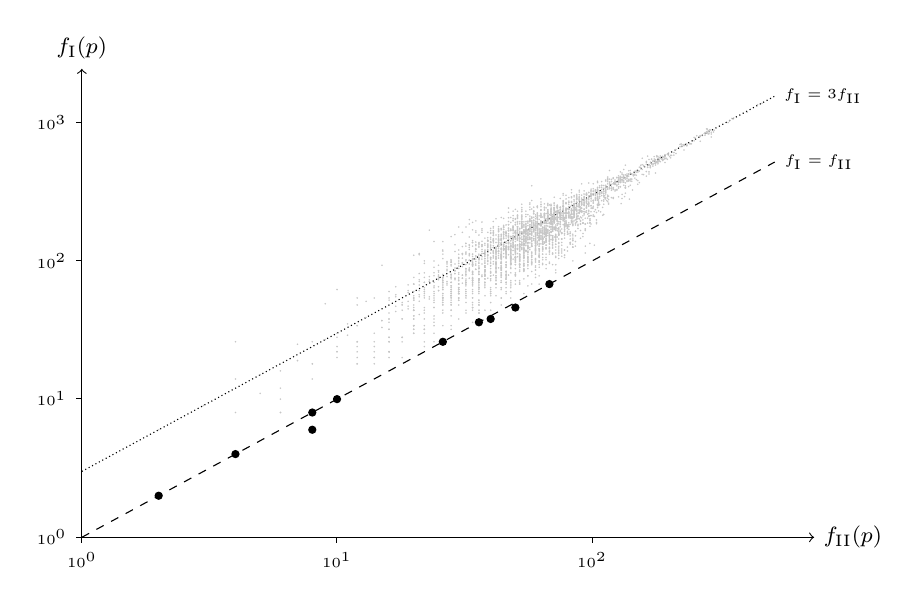
\begin{tikzpicture}[x=1cm,y=1cm]
\draw[->] (0,0) -- (9.30,0) node[right]{\footnotesize $\fII(p)$};
\draw[->] (0,0) -- (0,5.95) node[above]{\footnotesize $\fI(p)$};
\draw (0.00,0) -- (0.00,-0.07) node[below]{\tiny $10^{0}$};
\draw (3.24,0) -- (3.24,-0.07) node[below]{\tiny $10^{1}$};
\draw (6.48,0) -- (6.48,-0.07) node[below]{\tiny $10^{2}$};
\draw (0,0.00) -- (-0.07,0.00) node[left]{\tiny $10^{0}$};
\draw (0,1.76) -- (-0.07,1.76) node[left]{\tiny $10^{1}$};
\draw (0,3.51) -- (-0.07,3.51) node[left]{\tiny $10^{2}$};
\draw (0,5.27) -- (-0.07,5.27) node[left]{\tiny $10^{3}$};
\draw[dashed] (0.000,0.000) -- (8.800,4.766) node[right]{\tiny $\fI=\fII$};
\draw[densely dotted] (0.000,0.837) -- (8.794,5.600) node[right]{\tiny $\fI=3\fII$};
\fill[gray!45] (1.546,1.675) circle (0.32pt);
\fill[gray!45] (2.265,1.828) circle (0.32pt);
\fill[gray!45] (0.976,1.366) circle (0.32pt);
\fill[gray!45] (2.265,2.064) circle (0.32pt);
\fill[gray!45] (3.375,2.567) circle (0.32pt);
\fill[gray!45] (2.522,1.585) circle (0.32pt);
\fill[gray!45] (3.092,2.512) circle (0.32pt);
\fill[gray!45] (1.951,2.011) circle (0.32pt);
\fill[gray!45] (2.739,2.244) circle (0.32pt);
\fill[gray!45] (4.144,2.935) circle (0.32pt);
\fill[gray!45] (2.927,2.203) circle (0.32pt);
\fill[gray!45] (3.811,2.752) circle (0.32pt);
\fill[gray!45] (2.522,2.113) circle (0.32pt);
\fill[gray!45] (2.739,2.453) circle (0.32pt);
\fill[gray!45] (4.285,3.082) circle (0.32pt);
\fill[gray!45] (2.522,1.585) circle (0.32pt);
\fill[gray!45] (3.987,3.054) circle (0.32pt);
\fill[gray!45] (3.610,2.792) circle (0.32pt);
\fill[gray!45] (2.522,1.755) circle (0.32pt);
\fill[gray!45] (3.714,2.203) circle (0.32pt);
\fill[gray!45] (3.811,2.752) circle (0.32pt);
\fill[gray!45] (3.811,2.665) circle (0.32pt);
\fill[gray!45] (3.241,2.283) circle (0.32pt);
\fill[gray!45] (2.927,2.203) circle (0.32pt);
\fill[gray!45] (3.610,2.997) circle (0.32pt);
\fill[gray!45] (4.285,2.830) circle (0.32pt);
\fill[gray!45] (3.497,2.356) circle (0.32pt);
\fill[gray!45] (4.144,2.997) circle (0.32pt);
\fill[gray!45] (3.497,2.422) circle (0.32pt);
\fill[gray!45] (3.987,2.867) circle (0.32pt);
\fill[gray!45] (3.902,2.642) circle (0.32pt);
\fill[gray!45] (3.375,2.710) circle (0.32pt);
\fill[gray!45] (4.921,3.471) circle (0.32pt);
\fill[gray!45] (3.902,2.731) circle (0.32pt);
\fill[gray!45] (4.285,3.249) circle (0.32pt);
\fill[gray!45] (2.927,2.483) circle (0.32pt);
\fill[gray!45] (5.082,3.471) circle (0.32pt);
\fill[gray!45] (1.951,1.585) circle (0.32pt);
\fill[gray!45] (3.497,2.688) circle (0.32pt);
\fill[gray!45] (4.285,3.133) circle (0.32pt);
\fill[gray!45] (3.092,2.966) circle (0.32pt);
\fill[gray!45] (4.739,3.386) circle (0.32pt);
\fill[gray!45] (4.285,2.997) circle (0.32pt);
\fill[gray!45] (3.241,2.592) circle (0.32pt);
\fill[gray!45] (3.497,2.483) circle (0.32pt);
\fill[gray!45] (5.588,3.854) circle (0.32pt);
\fill[gray!45] (4.833,3.227) circle (0.32pt);
\fill[gray!45] (3.902,2.356) circle (0.32pt);
\fill[gray!45] (5.082,3.533) circle (0.32pt);
\fill[gray!45] (4.068,2.773) circle (0.32pt);
\fill[gray!45] (4.638,3.205) circle (0.32pt);
\fill[gray!45] (4.068,2.884) circle (0.32pt);
\fill[gray!45] (3.714,2.283) circle (0.32pt);
\fill[gray!45] (4.144,2.901) circle (0.32pt);
\fill[gray!45] (4.068,2.982) circle (0.32pt);
\fill[gray!45] (4.413,3.054) circle (0.32pt);
\fill[gray!45] (5.293,3.603) circle (0.32pt);
\fill[gray!45] (3.241,2.356) circle (0.32pt);
\fill[gray!45] (4.216,2.951) circle (0.32pt);
\fill[gray!45] (3.987,3.082) circle (0.32pt);
\fill[gray!45] (3.902,2.483) circle (0.32pt);
\fill[gray!45] (4.413,3.026) circle (0.32pt);
\fill[gray!45] (4.216,2.884) circle (0.32pt);
\fill[gray!45] (3.714,2.422) circle (0.32pt);
\fill[gray!45] (5.640,3.882) circle (0.32pt);
\fill[gray!45] (4.285,3.349) circle (0.32pt);
\fill[gray!45] (3.497,3.040) circle (0.32pt);
\fill[gray!45] (4.285,3.054) circle (0.32pt);
\fill[gray!45] (5.293,3.692) circle (0.32pt);
\fill[gray!45] (4.216,2.812) circle (0.32pt);
\fill[gray!45] (3.902,2.849) circle (0.32pt);
\fill[gray!45] (4.068,2.540) circle (0.32pt);
\fill[gray!45] (3.497,2.203) circle (0.32pt);
\fill[gray!45] (5.293,3.630) circle (0.32pt);
\fill[gray!45] (3.241,2.356) circle (0.32pt);
\fill[gray!45] (5.477,3.739) circle (0.32pt);
\fill[gray!45] (4.068,2.283) circle (0.32pt);
\fill[gray!45] (5.082,3.655) circle (0.32pt);
\fill[gray!45] (4.144,3.108) circle (0.32pt);
\fill[gray!45] (3.497,2.203) circle (0.32pt);
\fill[gray!45] (3.714,2.283) circle (0.32pt);
\fill[gray!45] (4.473,2.688) circle (0.32pt);
\fill[gray!45] (4.530,3.270) circle (0.32pt);
\fill[gray!45] (4.833,3.330) circle (0.32pt);
\fill[gray!45] (6.076,4.121) circle (0.32pt);
\fill[gray!45] (3.987,3.182) circle (0.32pt);
\fill[gray!45] (4.739,3.291) circle (0.32pt);
\fill[gray!45] (4.285,3.205) circle (0.32pt);
\fill[gray!45] (5.690,3.854) circle (0.32pt);
\fill[gray!45] (4.350,2.884) circle (0.32pt);
\fill[gray!45] (4.473,2.773) circle (0.32pt);
\fill[gray!45] (4.530,3.133) circle (0.32pt);
\fill[gray!45] (3.497,2.951) circle (0.32pt);
\fill[gray!45] (3.987,2.935) circle (0.32pt);
\fill[gray!45] (4.963,3.301) circle (0.32pt);
\fill[gray!45] (4.530,3.133) circle (0.32pt);
\fill[gray!45] (4.473,2.731) circle (0.32pt);
\fill[gray!45] (4.530,3.386) circle (0.32pt);
\fill[gray!45] (3.714,2.356) circle (0.32pt);
\fill[gray!45] (4.833,3.291) circle (0.32pt);
\fill[gray!45] (4.068,2.483) circle (0.32pt);
\fill[gray!45] (5.785,3.928) circle (0.32pt);
\fill[gray!45] (3.497,2.283) circle (0.32pt);
\fill[gray!45] (5.156,3.471) circle (0.32pt);
\fill[gray!45] (4.216,3.216) circle (0.32pt);
\fill[gray!45] (4.068,2.951) circle (0.32pt);
\fill[gray!45] (4.739,3.270) circle (0.32pt);
\fill[gray!45] (4.144,3.133) circle (0.32pt);
\fill[gray!45] (4.690,2.812) circle (0.32pt);
\fill[gray!45] (4.638,3.249) circle (0.32pt);
\fill[gray!45] (5.293,3.643) circle (0.32pt);
\fill[gray!45] (4.216,3.121) circle (0.32pt);
\fill[gray!45] (5.357,3.655) circle (0.32pt);
\fill[gray!45] (4.350,2.849) circle (0.32pt);
\fill[gray!45] (3.241,2.422) circle (0.32pt);
\fill[gray!45] (4.585,3.193) circle (0.32pt);
\fill[gray!45] (4.413,3.311) circle (0.32pt);
\fill[gray!45] (4.144,3.205) circle (0.32pt);
\fill[gray!45] (5.043,2.951) circle (0.32pt);
\fill[gray!45] (3.902,3.121) circle (0.32pt);
\fill[gray!45] (6.317,4.218) circle (0.32pt);
\fill[gray!45] (5.156,3.643) circle (0.32pt);
\fill[gray!45] (4.585,3.238) circle (0.32pt);
\fill[gray!45] (4.285,3.603) circle (0.32pt);
\fill[gray!45] (5.004,3.655) circle (0.32pt);
\fill[gray!45] (4.530,3.455) circle (0.32pt);
\fill[gray!45] (4.216,3.040) circle (0.32pt);
\fill[gray!45] (4.350,2.483) circle (0.32pt);
\fill[gray!45] (3.902,2.283) circle (0.32pt);
\fill[gray!45] (4.473,3.095) circle (0.32pt);
\fill[gray!45] (4.638,3.227) circle (0.32pt);
\fill[gray!45] (4.963,3.216) circle (0.32pt);
\fill[gray!45] (4.473,2.982) circle (0.32pt);
\fill[gray!45] (4.921,3.291) circle (0.32pt);
\fill[gray!45] (4.690,3.095) circle (0.32pt);
\fill[gray!45] (4.530,3.291) circle (0.32pt);
\fill[gray!45] (4.833,3.487) circle (0.32pt);
\fill[gray!45] (4.787,3.260) circle (0.32pt);
\fill[gray!45] (6.379,4.329) circle (0.32pt);
\fill[gray!45] (3.902,3.012) circle (0.32pt);
\fill[gray!45] (4.690,2.884) circle (0.32pt);
\fill[gray!45] (4.638,3.311) circle (0.32pt);
\fill[gray!45] (5.690,3.945) circle (0.32pt);
\fill[gray!45] (4.963,3.377) circle (0.32pt);
\fill[gray!45] (4.963,2.731) circle (0.32pt);
\fill[gray!45] (4.413,3.270) circle (0.32pt);
\fill[gray!45] (5.419,3.655) circle (0.32pt);
\fill[gray!45] (4.530,3.182) circle (0.32pt);
\fill[gray!45] (5.785,3.971) circle (0.32pt);
\fill[gray!45] (5.293,3.716) circle (0.32pt);
\fill[gray!45] (4.350,2.773) circle (0.32pt);
\fill[gray!45] (4.350,2.642) circle (0.32pt);
\fill[gray!45] (4.878,2.884) circle (0.32pt);
\fill[gray!45] (4.413,3.249) circle (0.32pt);
\fill[gray!45] (4.690,3.040) circle (0.32pt);
\fill[gray!45] (4.638,3.386) circle (0.32pt);
\fill[gray!45] (5.156,3.291) circle (0.32pt);
\fill[gray!45] (4.216,3.068) circle (0.32pt);
\fill[gray!45] (5.477,3.643) circle (0.32pt);
\fill[gray!45] (4.921,3.590) circle (0.32pt);
\fill[gray!45] (4.585,3.238) circle (0.32pt);
\fill[gray!45] (3.902,2.356) circle (0.32pt);
\fill[gray!45] (3.902,3.040) circle (0.32pt);
\fill[gray!45] (5.477,3.704) circle (0.32pt);
\fill[gray!45] (4.216,3.012) circle (0.32pt);
\fill[gray!45] (5.640,3.727) circle (0.32pt);
\fill[gray!45] (4.216,2.884) circle (0.32pt);
\fill[gray!45] (5.640,4.011) circle (0.32pt);
\fill[gray!45] (5.043,2.849) circle (0.32pt);
\fill[gray!45] (4.739,3.386) circle (0.32pt);
\fill[gray!45] (4.787,3.216) circle (0.32pt);
\fill[gray!45] (5.357,3.692) circle (0.32pt);
\fill[gray!45] (4.690,3.068) circle (0.32pt);
\fill[gray!45] (5.156,3.804) circle (0.32pt);
\fill[gray!45] (5.419,3.783) circle (0.32pt);
\fill[gray!45] (3.241,3.146) circle (0.32pt);
\fill[gray!45] (4.585,3.068) circle (0.32pt);
\fill[gray!45] (5.690,3.901) circle (0.32pt);
\fill[gray!45] (4.585,3.012) circle (0.32pt);
\fill[gray!45] (5.260,3.395) circle (0.32pt);
\fill[gray!45] (4.285,3.270) circle (0.32pt);
\fill[gray!45] (3.241,2.540) circle (0.32pt);
\fill[gray!45] (6.076,4.101) circle (0.32pt);
\fill[gray!45] (3.902,2.540) circle (0.32pt);
\fill[gray!45] (4.530,3.311) circle (0.32pt);
\fill[gray!45] (4.530,3.368) circle (0.32pt);
\fill[gray!45] (5.043,3.095) circle (0.32pt);
\fill[gray!45] (5.226,3.617) circle (0.32pt);
\fill[gray!45] (5.192,3.095) circle (0.32pt);
\fill[gray!45] (2.927,2.011) circle (0.32pt);
\fill[gray!45] (4.350,3.510) circle (0.32pt);
\fill[gray!45] (4.787,3.095) circle (0.32pt);
\fill[gray!45] (5.831,3.979) circle (0.32pt);
\fill[gray!45] (5.119,3.281) circle (0.32pt);
\fill[gray!45] (5.785,3.954) circle (0.32pt);
\fill[gray!45] (4.473,3.359) circle (0.32pt);
\fill[gray!45] (3.902,2.356) circle (0.32pt);
\fill[gray!45] (5.831,3.987) circle (0.32pt);
\fill[gray!45] (4.787,3.216) circle (0.32pt);
\fill[gray!45] (5.588,3.945) circle (0.32pt);
\fill[gray!45] (5.082,3.330) circle (0.32pt);
\fill[gray!45] (4.585,3.012) circle (0.32pt);
\fill[gray!45] (4.921,3.386) circle (0.32pt);
\fill[gray!45] (4.068,2.773) circle (0.32pt);
\fill[gray!45] (4.585,2.982) circle (0.32pt);
\fill[gray!45] (4.530,3.330) circle (0.32pt);
\fill[gray!45] (5.004,3.455) circle (0.32pt);
\fill[gray!45] (6.467,4.329) circle (0.32pt);
\fill[gray!45] (3.902,2.540) circle (0.32pt);
\fill[gray!45] (4.921,3.421) circle (0.32pt);
\fill[gray!45] (5.119,2.884) circle (0.32pt);
\fill[gray!45] (5.785,3.945) circle (0.32pt);
\fill[gray!45] (4.473,3.121) circle (0.32pt);
\fill[gray!45] (3.714,3.040) circle (0.32pt);
\fill[gray!45] (5.959,3.987) circle (0.32pt);
\fill[gray!45] (3.902,2.773) circle (0.32pt);
\fill[gray!45] (5.156,3.518) circle (0.32pt);
\fill[gray!45] (5.588,3.727) circle (0.32pt);
\fill[gray!45] (4.350,3.095) circle (0.32pt);
\fill[gray!45] (4.963,3.238) circle (0.32pt);
\fill[gray!45] (6.749,4.489) circle (0.32pt);
\fill[gray!45] (4.530,3.386) circle (0.32pt);
\fill[gray!45] (5.293,3.421) circle (0.32pt);
\fill[gray!45] (4.690,3.301) circle (0.32pt);
\fill[gray!45] (4.638,3.404) circle (0.32pt);
\fill[gray!45] (5.357,3.655) circle (0.32pt);
\fill[gray!45] (5.192,3.068) circle (0.32pt);
\fill[gray!45] (5.004,3.404) circle (0.32pt);
\fill[gray!45] (5.999,3.937) circle (0.32pt);
\fill[gray!45] (3.714,2.592) circle (0.32pt);
\fill[gray!45] (5.043,3.583) circle (0.32pt);
\fill[gray!45] (5.293,3.716) circle (0.32pt);
\fill[gray!45] (6.348,4.253) circle (0.32pt);
\fill[gray!45] (3.811,3.455) circle (0.32pt);
\fill[gray!45] (4.638,3.438) circle (0.32pt);
\fill[gray!45] (4.833,3.291) circle (0.32pt);
\fill[gray!45] (4.350,3.121) circle (0.32pt);
\fill[gray!45] (4.690,3.193) circle (0.32pt);
\fill[gray!45] (6.602,4.380) circle (0.32pt);
\fill[gray!45] (5.533,3.892) circle (0.32pt);
\fill[gray!45] (5.082,3.311) circle (0.32pt);
\fill[gray!45] (5.226,3.630) circle (0.32pt);
\fill[gray!45] (6.317,4.270) circle (0.32pt);
\fill[gray!45] (4.878,3.321) circle (0.32pt);
\fill[gray!45] (4.473,2.812) circle (0.32pt);
\fill[gray!45] (5.226,3.680) circle (0.32pt);
\fill[gray!45] (4.350,2.642) circle (0.32pt);
\fill[gray!45] (4.690,3.193) circle (0.32pt);
\fill[gray!45] (5.533,3.824) circle (0.32pt);
\fill[gray!45] (4.350,3.238) circle (0.32pt);
\fill[gray!45] (5.156,3.547) circle (0.32pt);
\fill[gray!45] (4.963,3.281) circle (0.32pt);
\fill[gray!45] (4.690,3.068) circle (0.32pt);
\fill[gray!45] (5.477,3.937) circle (0.32pt);
\fill[gray!45] (5.226,3.502) circle (0.32pt);
\fill[gray!45] (5.043,3.413) circle (0.32pt);
\fill[gray!45] (4.690,3.121) circle (0.32pt);
\fill[gray!45] (4.787,3.216) circle (0.32pt);
\fill[gray!45] (4.921,3.680) circle (0.32pt);
\fill[gray!45] (4.787,3.095) circle (0.32pt);
\fill[gray!45] (5.043,2.982) circle (0.32pt);
\fill[gray!45] (4.739,3.349) circle (0.32pt);
\fill[gray!45] (4.878,3.395) circle (0.32pt);
\fill[gray!45] (4.216,3.216) circle (0.32pt);
\fill[gray!45] (4.921,3.655) circle (0.32pt);
\fill[gray!45] (4.787,3.040) circle (0.32pt);
\fill[gray!45] (6.285,4.212) circle (0.32pt);
\fill[gray!45] (4.216,2.884) circle (0.32pt);
\fill[gray!45] (4.833,3.330) circle (0.32pt);
\fill[gray!45] (4.833,3.471) circle (0.32pt);
\fill[gray!45] (4.963,3.463) circle (0.32pt);
\fill[gray!45] (4.350,2.422) circle (0.32pt);
\fill[gray!45] (5.419,3.330) circle (0.32pt);
\fill[gray!45] (6.409,4.199) circle (0.32pt);
\fill[gray!45] (4.833,3.603) circle (0.32pt);
\fill[gray!45] (6.495,4.365) circle (0.32pt);
\fill[gray!45] (4.350,3.121) circle (0.32pt);
\fill[gray!45] (4.921,3.386) circle (0.32pt);
\fill[gray!45] (6.348,4.270) circle (0.32pt);
\fill[gray!45] (3.902,2.483) circle (0.32pt);
\fill[gray!45] (4.690,3.281) circle (0.32pt);
\fill[gray!45] (5.293,3.783) circle (0.32pt);
\fill[gray!45] (5.260,3.216) circle (0.32pt);
\fill[gray!45] (5.326,3.495) circle (0.32pt);
\fill[gray!45] (5.004,3.471) circle (0.32pt);
\fill[gray!45] (4.878,3.238) circle (0.32pt);
\fill[gray!45] (5.640,3.793) circle (0.32pt);
\fill[gray!45] (4.585,3.340) circle (0.32pt);
\fill[gray!45] (5.388,3.463) circle (0.32pt);
\fill[gray!45] (5.419,3.680) circle (0.32pt);
\fill[gray!45] (5.192,3.359) circle (0.32pt);
\fill[gray!45] (6.076,4.035) circle (0.32pt);
\fill[gray!45] (4.921,3.404) circle (0.32pt);
\fill[gray!45] (4.216,3.012) circle (0.32pt);
\fill[gray!45] (5.119,3.321) circle (0.32pt);
\fill[gray!45] (5.588,3.945) circle (0.32pt);
\fill[gray!45] (4.739,3.386) circle (0.32pt);
\fill[gray!45] (5.293,3.576) circle (0.32pt);
\fill[gray!45] (3.902,2.773) circle (0.32pt);
\fill[gray!45] (5.082,3.562) circle (0.32pt);
\fill[gray!45] (4.585,3.170) circle (0.32pt);
\fill[gray!45] (6.467,4.340) circle (0.32pt);
\fill[gray!45] (4.585,3.636) circle (0.32pt);
\fill[gray!45] (5.959,4.011) circle (0.32pt);
\fill[gray!45] (5.192,3.413) circle (0.32pt);
\fill[gray!45] (4.585,2.884) circle (0.32pt);
\fill[gray!45] (4.285,3.590) circle (0.32pt);
\fill[gray!45] (5.875,4.019) circle (0.32pt);
\fill[gray!45] (4.585,2.688) circle (0.32pt);
\fill[gray!45] (5.999,4.072) circle (0.32pt);
\fill[gray!45] (6.523,4.394) circle (0.32pt);
\fill[gray!45] (4.690,2.951) circle (0.32pt);
\fill[gray!45] (4.878,3.068) circle (0.32pt);
\fill[gray!45] (5.156,3.502) circle (0.32pt);
\fill[gray!45] (4.585,2.951) circle (0.32pt);
\fill[gray!45] (5.326,3.340) circle (0.32pt);
\fill[gray!45] (5.357,3.704) circle (0.32pt);
\fill[gray!45] (5.119,3.377) circle (0.32pt);
\fill[gray!45] (4.473,2.483) circle (0.32pt);
\fill[gray!45] (5.156,3.590) circle (0.32pt);
\fill[gray!45] (5.082,3.603) circle (0.32pt);
\fill[gray!45] (6.252,4.187) circle (0.32pt);
\fill[gray!45] (4.690,3.238) circle (0.32pt);
\fill[gray!45] (4.216,3.301) circle (0.32pt);
\fill[gray!45] (5.762,3.767) circle (0.32pt);
\fill[gray!45] (6.467,4.404) circle (0.32pt);
\fill[gray!45] (5.226,3.761) circle (0.32pt);
\fill[gray!45] (4.739,3.349) circle (0.32pt);
\fill[gray!45] (5.588,3.783) circle (0.32pt);
\fill[gray!45] (4.473,3.430) circle (0.32pt);
\fill[gray!45] (4.963,3.377) circle (0.32pt);
\fill[gray!45] (4.216,2.688) circle (0.32pt);
\fill[gray!45] (5.999,4.035) circle (0.32pt);
\fill[gray!45] (4.690,3.495) circle (0.32pt);
\fill[gray!45] (4.585,3.170) circle (0.32pt);
\fill[gray!45] (4.963,3.121) circle (0.32pt);
\fill[gray!45] (4.833,3.692) circle (0.32pt);
\fill[gray!45] (5.119,3.495) circle (0.32pt);
\fill[gray!45] (5.875,4.114) circle (0.32pt);
\fill[gray!45] (4.473,3.012) circle (0.32pt);
\fill[gray!45] (4.739,3.421) circle (0.32pt);
\fill[gray!45] (6.550,4.308) circle (0.32pt);
\fill[gray!45] (4.963,3.447) circle (0.32pt);
\fill[gray!45] (5.357,3.668) circle (0.32pt);
\fill[gray!45] (4.787,3.170) circle (0.32pt);
\fill[gray!45] (4.473,3.170) circle (0.32pt);
\fill[gray!45] (5.226,3.562) circle (0.32pt);
\fill[gray!45] (4.963,3.447) circle (0.32pt);
\fill[gray!45] (5.192,3.281) circle (0.32pt);
\fill[gray!45] (6.839,4.505) circle (0.32pt);
\fill[gray!45] (5.419,3.655) circle (0.32pt);
\fill[gray!45] (4.350,3.301) circle (0.32pt);
\fill[gray!45] (5.156,3.772) circle (0.32pt);
\fill[gray!45] (5.043,3.260) circle (0.32pt);
\fill[gray!45] (5.506,3.321) circle (0.32pt);
\fill[gray!45] (6.467,4.370) circle (0.32pt);
\fill[gray!45] (5.875,3.873) circle (0.32pt);
\fill[gray!45] (4.530,3.291) circle (0.32pt);
\fill[gray!45] (4.068,2.951) circle (0.32pt);
\fill[gray!45] (5.388,3.569) circle (0.32pt);
\fill[gray!45] (5.004,3.630) circle (0.32pt);
\fill[gray!45] (2.522,1.894) circle (0.32pt);
\fill[gray!45] (4.739,3.291) circle (0.32pt);
\fill[gray!45] (4.833,3.438) circle (0.32pt);
\fill[gray!45] (5.785,3.995) circle (0.32pt);
\fill[gray!45] (5.260,3.301) circle (0.32pt);
\fill[gray!45] (5.640,3.892) circle (0.32pt);
\fill[gray!45] (5.119,3.479) circle (0.32pt);
\fill[gray!45] (5.918,3.864) circle (0.32pt);
\fill[gray!45] (6.438,4.308) circle (0.32pt);
\fill[gray!45] (4.878,3.068) circle (0.32pt);
\fill[gray!45] (5.043,2.884) circle (0.32pt);
\fill[gray!45] (4.787,2.951) circle (0.32pt);
\fill[gray!45] (5.388,3.359) circle (0.32pt);
\fill[gray!45] (4.878,3.377) circle (0.32pt);
\fill[gray!45] (4.739,3.471) circle (0.32pt);
\fill[gray!45] (4.963,3.340) circle (0.32pt);
\fill[gray!45] (5.640,3.864) circle (0.32pt);
\fill[gray!45] (5.918,4.035) circle (0.32pt);
\fill[gray!45] (4.921,3.576) circle (0.32pt);
\fill[gray!45] (5.043,3.540) circle (0.32pt);
\fill[gray!45] (5.588,3.655) circle (0.32pt);
\fill[gray!45] (6.749,4.489) circle (0.32pt);
\fill[gray!45] (4.068,2.540) circle (0.32pt);
\fill[gray!45] (5.043,3.340) circle (0.32pt);
\fill[gray!45] (5.785,3.945) circle (0.32pt);
\fill[gray!45] (4.638,3.471) circle (0.32pt);
\fill[gray!45] (5.640,3.864) circle (0.32pt);
\fill[gray!45] (4.585,3.146) circle (0.32pt);
\fill[gray!45] (6.149,4.235) circle (0.32pt);
\fill[gray!45] (5.192,3.281) circle (0.32pt);
\fill[gray!45] (4.921,3.518) circle (0.32pt);
\fill[gray!45] (4.878,3.413) circle (0.32pt);
\fill[gray!45] (5.192,3.447) circle (0.32pt);
\fill[gray!45] (4.963,3.359) circle (0.32pt);
\fill[gray!45] (5.419,3.692) circle (0.32pt);
\fill[gray!45] (4.878,3.193) circle (0.32pt);
\fill[gray!45] (5.119,3.281) circle (0.32pt);
\fill[gray!45] (5.226,3.547) circle (0.32pt);
\fill[gray!45] (5.614,3.610) circle (0.32pt);
\fill[gray!45] (5.260,3.216) circle (0.32pt);
\fill[gray!45] (5.226,3.471) circle (0.32pt);
\fill[gray!45] (5.640,3.750) circle (0.32pt);
\fill[gray!45] (4.216,2.884) circle (0.32pt);
\fill[gray!45] (4.787,3.596) circle (0.32pt);
\fill[gray!45] (5.226,3.704) circle (0.32pt);
\fill[gray!45] (5.357,3.739) circle (0.32pt);
\fill[gray!45] (4.690,3.146) circle (0.32pt);
\fill[gray!45] (4.963,3.216) circle (0.32pt);
\fill[gray!45] (7.098,4.685) circle (0.32pt);
\fill[gray!45] (4.921,3.716) circle (0.32pt);
\fill[gray!45] (5.119,3.377) circle (0.32pt);
\fill[gray!45] (6.149,4.065) circle (0.32pt);
\fill[gray!45] (5.808,3.510) circle (0.32pt);
\fill[gray!45] (4.585,3.216) circle (0.32pt);
\fill[gray!45] (5.739,3.995) circle (0.32pt);
\fill[gray!45] (6.185,4.079) circle (0.32pt);
\fill[gray!45] (4.690,3.121) circle (0.32pt);
\fill[gray!45] (5.506,3.569) circle (0.32pt);
\fill[gray!45] (5.690,3.793) circle (0.32pt);
\fill[gray!45] (5.043,3.193) circle (0.32pt);
\fill[gray!45] (5.004,3.404) circle (0.32pt);
\fill[gray!45] (6.438,4.259) circle (0.32pt);
\fill[gray!45] (5.043,2.951) circle (0.32pt);
\fill[gray!45] (5.293,3.750) circle (0.32pt);
\fill[gray!45] (5.357,3.793) circle (0.32pt);
\fill[gray!45] (6.817,4.522) circle (0.32pt);
\fill[gray!45] (5.388,3.623) circle (0.32pt);
\fill[gray!45] (4.963,2.918) circle (0.32pt);
\fill[gray!45] (4.216,2.592) circle (0.32pt);
\fill[gray!45] (4.690,3.321) circle (0.32pt);
\fill[gray!45] (5.082,3.630) circle (0.32pt);
\fill[gray!45] (6.576,4.329) circle (0.32pt);
\fill[gray!45] (4.921,3.404) circle (0.32pt);
\fill[gray!45] (4.585,3.281) circle (0.32pt);
\fill[gray!45] (4.690,3.510) circle (0.32pt);
\fill[gray!45] (7.098,4.726) circle (0.32pt);
\fill[gray!45] (4.585,2.849) circle (0.32pt);
\fill[gray!45] (4.350,3.146) circle (0.32pt);
\fill[gray!45] (5.357,3.716) circle (0.32pt);
\fill[gray!45] (6.772,4.509) circle (0.32pt);
\fill[gray!45] (3.497,2.483) circle (0.32pt);
\fill[gray!45] (5.043,3.281) circle (0.32pt);
\fill[gray!45] (5.156,3.680) circle (0.32pt);
\fill[gray!45] (6.726,4.408) circle (0.32pt);
\fill[gray!45] (4.739,3.716) circle (0.32pt);
\fill[gray!45] (5.388,3.238) circle (0.32pt);
\fill[gray!45] (5.119,3.238) circle (0.32pt);
\fill[gray!45] (5.043,3.260) circle (0.32pt);
\fill[gray!45] (4.963,3.463) circle (0.32pt);
\fill[gray!45] (5.357,3.603) circle (0.32pt);
\fill[gray!45] (5.192,3.610) circle (0.32pt);
\fill[gray!45] (4.963,3.495) circle (0.32pt);
\fill[gray!45] (5.156,3.692) circle (0.32pt);
\fill[gray!45] (5.156,3.727) circle (0.32pt);
\fill[gray!45] (6.285,4.072) circle (0.32pt);
\fill[gray!45] (5.043,3.377) circle (0.32pt);
\fill[gray!45] (5.293,3.630) circle (0.32pt);
\fill[gray!45] (4.963,2.918) circle (0.32pt);
\fill[gray!45] (5.533,3.844) circle (0.32pt);
\fill[gray!45] (5.226,3.643) circle (0.32pt);
\fill[gray!45] (5.326,3.170) circle (0.32pt);
\fill[gray!45] (5.588,3.680) circle (0.32pt);
\fill[gray!45] (5.999,4.086) circle (0.32pt);
\fill[gray!45] (5.477,3.750) circle (0.32pt);
\fill[gray!45] (7.532,4.917) circle (0.32pt);
\fill[gray!45] (1.951,2.483) circle (0.32pt);
\fill[gray!45] (5.477,3.533) circle (0.32pt);
\fill[gray!45] (4.963,3.495) circle (0.32pt);
\fill[gray!45] (4.963,3.359) circle (0.32pt);
\fill[gray!45] (5.640,3.814) circle (0.32pt);
\fill[gray!45] (5.999,4.072) circle (0.32pt);
\fill[gray!45] (5.326,3.569) circle (0.32pt);
\fill[gray!45] (4.690,2.884) circle (0.32pt);
\fill[gray!45] (5.388,3.281) circle (0.32pt);
\fill[gray!45] (4.878,2.982) circle (0.32pt);
\fill[gray!45] (5.506,3.321) circle (0.32pt);
\fill[gray!45] (5.004,3.533) circle (0.32pt);
\fill[gray!45] (5.640,3.704) circle (0.32pt);
\fill[gray!45] (5.119,3.447) circle (0.32pt);
\fill[gray!45] (5.533,3.562) circle (0.32pt);
\fill[gray!45] (5.690,3.844) circle (0.32pt);
\fill[gray!45] (5.293,3.739) circle (0.32pt);
\fill[gray!45] (5.808,3.767) circle (0.32pt);
\fill[gray!45] (6.523,4.365) circle (0.32pt);
\fill[gray!45] (3.902,2.642) circle (0.32pt);
\fill[gray!45] (5.326,3.554) circle (0.32pt);
\fill[gray!45] (5.690,3.882) circle (0.32pt);
\fill[gray!45] (4.473,3.321) circle (0.32pt);
\fill[gray!45] (5.226,3.330) circle (0.32pt);
\fill[gray!45] (5.260,3.430) circle (0.32pt);
\fill[gray!45] (5.477,3.954) circle (0.32pt);
\fill[gray!45] (5.156,3.655) circle (0.32pt);
\fill[gray!45] (5.614,3.610) circle (0.32pt);
\fill[gray!45] (6.113,4.072) circle (0.32pt);
\fill[gray!45] (5.119,3.596) circle (0.32pt);
\fill[gray!45] (5.739,3.882) circle (0.32pt);
\fill[gray!45] (4.787,3.540) circle (0.32pt);
\fill[gray!45] (5.260,3.170) circle (0.32pt);
\fill[gray!45] (5.533,3.814) circle (0.32pt);
\fill[gray!45] (5.477,3.834) circle (0.32pt);
\fill[gray!45] (5.762,3.868) circle (0.32pt);
\fill[gray!45] (5.226,3.761) circle (0.32pt);
\fill[gray!45] (5.831,3.864) circle (0.32pt);
\fill[gray!45] (6.628,4.270) circle (0.32pt);
\fill[gray!45] (5.043,3.281) circle (0.32pt);
\fill[gray!45] (5.561,3.756) circle (0.32pt);
\fill[gray!45] (5.477,3.814) circle (0.32pt);
\fill[gray!45] (5.043,2.884) circle (0.32pt);
\fill[gray!45] (5.388,3.170) circle (0.32pt);
\fill[gray!45] (5.448,3.698) circle (0.32pt);
\fill[gray!45] (6.628,4.432) circle (0.32pt);
\fill[gray!45] (5.082,3.716) circle (0.32pt);
\fill[gray!45] (4.878,3.698) circle (0.32pt);
\fill[gray!45] (5.959,4.108) circle (0.32pt);
\fill[gray!45] (5.119,3.170) circle (0.32pt);
\fill[gray!45] (5.477,3.901) circle (0.32pt);
\fill[gray!45] (4.690,3.170) circle (0.32pt);
\fill[gray!45] (6.495,4.281) circle (0.32pt);
\fill[gray!45] (4.878,3.146) circle (0.32pt);
\fill[gray!45] (5.506,3.596) circle (0.32pt);
\fill[gray!45] (5.293,3.547) circle (0.32pt);
\fill[gray!45] (5.260,3.321) circle (0.32pt);
\fill[gray!45] (5.293,3.824) circle (0.32pt);
\fill[gray!45] (5.119,3.540) circle (0.32pt);
\fill[gray!45] (5.533,3.910) circle (0.32pt);
\fill[gray!45] (5.477,3.716) circle (0.32pt);
\fill[gray!45] (4.963,3.260) circle (0.32pt);
\fill[gray!45] (6.550,4.365) circle (0.32pt);
\fill[gray!45] (4.585,3.238) circle (0.32pt);
\fill[gray!45] (5.326,3.040) circle (0.32pt);
\fill[gray!45] (4.216,2.773) circle (0.32pt);
\fill[gray!45] (4.638,3.487) circle (0.32pt);
\fill[gray!45] (6.038,4.057) circle (0.32pt);
\fill[gray!45] (5.665,3.686) circle (0.32pt);
\fill[gray!45] (6.409,4.370) circle (0.32pt);
\fill[gray!45] (5.477,3.692) circle (0.32pt);
\fill[gray!45] (5.561,3.260) circle (0.32pt);
\fill[gray!45] (5.226,3.834) circle (0.32pt);
\fill[gray!45] (5.640,3.971) circle (0.32pt);
\fill[gray!45] (5.831,3.873) circle (0.32pt);
\fill[gray!45] (5.739,3.971) circle (0.32pt);
\fill[gray!45] (5.326,3.569) circle (0.32pt);
\fill[gray!45] (5.506,3.463) circle (0.32pt);
\fill[gray!45] (5.739,3.937) circle (0.32pt);
\fill[gray!45] (5.640,3.864) circle (0.32pt);
\fill[gray!45] (5.043,3.525) circle (0.32pt);
\fill[gray!45] (5.785,3.864) circle (0.32pt);
\fill[gray!45] (5.119,3.583) circle (0.32pt);
\fill[gray!45] (5.690,3.783) circle (0.32pt);
\fill[gray!45] (4.878,3.121) circle (0.32pt);
\fill[gray!45] (5.004,3.502) circle (0.32pt);
\fill[gray!45] (4.963,3.238) circle (0.32pt);
\fill[gray!45] (5.561,3.569) circle (0.32pt);
\fill[gray!45] (7.220,4.694) circle (0.32pt);
\fill[gray!45] (5.999,3.814) circle (0.32pt);
\fill[gray!45] (4.963,3.569) circle (0.32pt);
\fill[gray!45] (5.226,3.854) circle (0.32pt);
\fill[gray!45] (5.156,3.873) circle (0.32pt);
\fill[gray!45] (6.409,4.247) circle (0.32pt);
\fill[gray!45] (4.690,2.642) circle (0.32pt);
\fill[gray!45] (5.388,3.554) circle (0.32pt);
\fill[gray!45] (6.185,4.174) circle (0.32pt);
\fill[gray!45] (4.787,3.359) circle (0.32pt);
\fill[gray!45] (6.019,3.756) circle (0.32pt);
\fill[gray!45] (6.550,4.389) circle (0.32pt);
\fill[gray!45] (5.388,3.340) circle (0.32pt);
\fill[gray!45] (3.714,2.483) circle (0.32pt);
\fill[gray!45] (5.739,3.910) circle (0.32pt);
\fill[gray!45] (5.388,3.447) circle (0.32pt);
\fill[gray!45] (5.477,3.772) circle (0.32pt);
\fill[gray!45] (4.963,3.340) circle (0.32pt);
\fill[gray!45] (5.357,3.844) circle (0.32pt);
\fill[gray!45] (5.326,3.040) circle (0.32pt);
\fill[gray!45] (5.082,3.704) circle (0.32pt);
\fill[gray!45] (5.665,3.839) circle (0.32pt);
\fill[gray!45] (5.831,3.901) circle (0.32pt);
\fill[gray!45] (4.585,3.596) circle (0.32pt);
\fill[gray!45] (6.285,4.042) circle (0.32pt);
\fill[gray!45] (4.963,3.146) circle (0.32pt);
\fill[gray!45] (6.076,4.121) circle (0.32pt);
\fill[gray!45] (5.448,3.040) circle (0.32pt);
\fill[gray!45] (5.119,3.430) circle (0.32pt);
\fill[gray!45] (4.833,3.547) circle (0.32pt);
\fill[gray!45] (5.043,3.447) circle (0.32pt);
\fill[gray!45] (5.831,3.962) circle (0.32pt);
\fill[gray!45] (5.260,3.623) circle (0.32pt);
\fill[gray!45] (5.043,3.540) circle (0.32pt);
\fill[gray!45] (5.785,3.739) circle (0.32pt);
\fill[gray!45] (4.690,3.495) circle (0.32pt);
\fill[gray!45] (6.113,4.199) circle (0.32pt);
\fill[gray!45] (5.808,3.809) circle (0.32pt);
\fill[gray!45] (5.326,3.146) circle (0.32pt);
\fill[gray!45] (5.561,3.510) circle (0.32pt);
\fill[gray!45] (5.477,3.892) circle (0.32pt);
\fill[gray!45] (5.326,2.951) circle (0.32pt);
\fill[gray!45] (5.293,3.844) circle (0.32pt);
\fill[gray!45] (5.831,3.834) circle (0.32pt);
\fill[gray!45] (5.388,3.623) circle (0.32pt);
\fill[gray!45] (6.602,4.375) circle (0.32pt);
\fill[gray!45] (5.448,3.193) circle (0.32pt);
\fill[gray!45] (5.533,3.668) circle (0.32pt);
\fill[gray!45] (4.787,3.447) circle (0.32pt);
\fill[gray!45] (5.588,3.668) circle (0.32pt);
\fill[gray!45] (4.350,2.918) circle (0.32pt);
\fill[gray!45] (5.043,3.722) circle (0.32pt);
\fill[gray!45] (5.640,3.910) circle (0.32pt);
\fill[gray!45] (5.640,3.892) circle (0.32pt);
\fill[gray!45] (5.419,3.590) circle (0.32pt);
\fill[gray!45] (5.192,3.377) circle (0.32pt);
\fill[gray!45] (4.690,3.012) circle (0.32pt);
\fill[gray!45] (5.293,3.668) circle (0.32pt);
\fill[gray!45] (5.785,3.928) circle (0.32pt);
\fill[gray!45] (6.113,4.057) circle (0.32pt);
\fill[gray!45] (5.714,3.623) circle (0.32pt);
\fill[gray!45] (5.357,3.716) circle (0.32pt);
\fill[gray!45] (4.585,3.040) circle (0.32pt);
\fill[gray!45] (5.762,3.662) circle (0.32pt);
\fill[gray!45] (6.317,4.281) circle (0.32pt);
\fill[gray!45] (5.533,3.716) circle (0.32pt);
\fill[gray!45] (5.388,3.121) circle (0.32pt);
\fill[gray!45] (5.293,3.750) circle (0.32pt);
\fill[gray!45] (4.690,2.982) circle (0.32pt);
\fill[gray!45] (5.533,3.945) circle (0.32pt);
\fill[gray!45] (5.506,3.510) circle (0.32pt);
\fill[gray!45] (7.220,4.714) circle (0.32pt);
\fill[gray!45] (5.785,3.892) circle (0.32pt);
\fill[gray!45] (6.861,4.569) circle (0.32pt);
\fill[gray!45] (5.448,3.238) circle (0.32pt);
\fill[gray!45] (4.833,3.603) circle (0.32pt);
\fill[gray!45] (4.216,2.642) circle (0.32pt);
\fill[gray!45] (5.119,3.510) circle (0.32pt);
\fill[gray!45] (7.042,4.598) circle (0.32pt);
\fill[gray!45] (6.628,4.389) circle (0.32pt);
\fill[gray!45] (6.113,4.121) circle (0.32pt);
\fill[gray!45] (6.076,4.161) circle (0.32pt);
\fill[gray!45] (4.473,3.238) circle (0.32pt);
\fill[gray!45] (5.448,3.479) circle (0.32pt);
\fill[gray!45] (7.098,4.698) circle (0.32pt);
\fill[gray!45] (4.473,2.592) circle (0.32pt);
\fill[gray!45] (5.192,3.525) circle (0.32pt);
\fill[gray!45] (4.690,3.238) circle (0.32pt);
\fill[gray!45] (5.357,3.873) circle (0.32pt);
\fill[gray!45] (5.448,3.510) circle (0.32pt);
\fill[gray!45] (6.726,4.427) circle (0.32pt);
\fill[gray!45] (5.388,3.636) circle (0.32pt);
\fill[gray!45] (5.192,3.540) circle (0.32pt);
\fill[gray!45] (4.638,3.502) circle (0.32pt);
\fill[gray!45] (4.878,3.463) circle (0.32pt);
\fill[gray!45] (6.726,4.450) circle (0.32pt);
\fill[gray!45] (5.588,3.716) circle (0.32pt);
\fill[gray!45] (4.878,3.733) circle (0.32pt);
\fill[gray!45] (5.561,3.554) circle (0.32pt);
\fill[gray!45] (5.999,4.086) circle (0.32pt);
\fill[gray!45] (5.004,3.668) circle (0.32pt);
\fill[gray!45] (5.762,3.756) circle (0.32pt);
\fill[gray!45] (6.409,4.287) circle (0.32pt);
\fill[gray!45] (5.043,2.849) circle (0.32pt);
\fill[gray!45] (5.326,3.479) circle (0.32pt);
\fill[gray!45] (5.785,3.716) circle (0.32pt);
\fill[gray!45] (5.119,3.321) circle (0.32pt);
\fill[gray!45] (5.588,3.987) circle (0.32pt);
\fill[gray!45] (5.419,3.668) circle (0.32pt);
\fill[gray!45] (4.963,3.260) circle (0.32pt);
\fill[gray!45] (5.785,3.892) circle (0.32pt);
\fill[gray!45] (5.614,3.649) circle (0.32pt);
\fill[gray!45] (5.690,3.892) circle (0.32pt);
\fill[gray!45] (7.776,5.035) circle (0.32pt);
\fill[gray!45] (5.004,3.704) circle (0.32pt);
\fill[gray!45] (5.588,3.954) circle (0.32pt);
\fill[gray!45] (4.787,3.554) circle (0.32pt);
\fill[gray!45] (5.614,3.554) circle (0.32pt);
\fill[gray!45] (6.550,4.308) circle (0.32pt);
\fill[gray!45] (6.409,4.148) circle (0.32pt);
\fill[gray!45] (5.448,3.596) circle (0.32pt);
\fill[gray!45] (5.156,3.772) circle (0.32pt);
\fill[gray!45] (4.963,3.281) circle (0.32pt);
\fill[gray!45] (5.999,4.218) circle (0.32pt);
\fill[gray!45] (6.348,4.148) circle (0.32pt);
\fill[gray!45] (4.787,3.146) circle (0.32pt);
\fill[gray!45] (6.076,4.128) circle (0.32pt);
\fill[gray!45] (5.640,3.630) circle (0.32pt);
\fill[gray!45] (5.918,4.019) circle (0.32pt);
\fill[gray!45] (5.448,3.479) circle (0.32pt);
\fill[gray!45] (5.853,3.788) circle (0.32pt);
\fill[gray!45] (4.690,2.688) circle (0.32pt);
\fill[gray!45] (5.004,3.576) circle (0.32pt);
\fill[gray!45] (6.252,4.101) circle (0.32pt);
\fill[gray!45] (4.963,3.359) circle (0.32pt);
\fill[gray!45] (5.260,3.636) circle (0.32pt);
\fill[gray!45] (5.853,3.686) circle (0.32pt);
\fill[gray!45] (5.448,3.569) circle (0.32pt);
\fill[gray!45] (7.545,4.924) circle (0.32pt);
\fill[gray!45] (4.216,2.592) circle (0.32pt);
\fill[gray!45] (5.260,3.540) circle (0.32pt);
\fill[gray!45] (6.550,4.399) circle (0.32pt);
\fill[gray!45] (5.561,3.698) circle (0.32pt);
\fill[gray!45] (5.477,3.680) circle (0.32pt);
\fill[gray!45] (4.963,3.767) circle (0.32pt);
\fill[gray!45] (5.226,3.603) circle (0.32pt);
\fill[gray!45] (6.038,4.019) circle (0.32pt);
\fill[gray!45] (5.260,3.301) circle (0.32pt);
\fill[gray!45] (5.419,3.680) circle (0.32pt);
\fill[gray!45] (5.614,3.510) circle (0.32pt);
\fill[gray!45] (6.924,4.576) circle (0.32pt);
\fill[gray!45] (5.690,4.079) circle (0.32pt);
\fill[gray!45] (4.585,3.649) circle (0.32pt);
\fill[gray!45] (5.506,3.413) circle (0.32pt);
\fill[gray!45] (5.357,3.692) circle (0.32pt);
\fill[gray!45] (5.918,4.072) circle (0.32pt);
\fill[gray!45] (5.853,3.788) circle (0.32pt);
\fill[gray!45] (5.260,3.216) circle (0.32pt);
\fill[gray!45] (4.833,3.590) circle (0.32pt);
\fill[gray!45] (5.448,3.121) circle (0.32pt);
\fill[gray!45] (6.882,4.561) circle (0.32pt);
\fill[gray!45] (5.448,3.540) circle (0.32pt);
\fill[gray!45] (5.588,3.873) circle (0.32pt);
\fill[gray!45] (5.156,3.704) circle (0.32pt);
\fill[gray!45] (5.714,3.525) circle (0.32pt);
\fill[gray!45] (5.785,3.987) circle (0.32pt);
\fill[gray!45] (5.918,3.954) circle (0.32pt);
\fill[gray!45] (7.186,4.698) circle (0.32pt);
\fill[gray!45] (4.216,2.812) circle (0.32pt);
\fill[gray!45] (5.004,3.655) circle (0.32pt);
\fill[gray!45] (5.533,3.603) circle (0.32pt);
\fill[gray!45] (5.561,3.479) circle (0.32pt);
\fill[gray!45] (5.477,3.864) circle (0.32pt);
\fill[gray!45] (4.216,2.688) circle (0.32pt);
\fill[gray!45] (5.448,3.819) circle (0.32pt);
\fill[gray!45] (4.878,3.510) circle (0.32pt);
\fill[gray!45] (6.076,4.079) circle (0.32pt);
\fill[gray!45] (5.831,3.962) circle (0.32pt);
\fill[gray!45] (6.653,4.471) circle (0.32pt);
\fill[gray!45] (4.216,2.773) circle (0.32pt);
\fill[gray!45] (5.082,3.692) circle (0.32pt);
\fill[gray!45] (5.588,3.750) circle (0.32pt);
\fill[gray!45] (5.043,3.698) circle (0.32pt);
\fill[gray!45] (5.260,3.525) circle (0.32pt);
\fill[gray!45] (5.419,3.739) circle (0.32pt);
\fill[gray!45] (5.448,3.463) circle (0.32pt);
\fill[gray!45] (5.831,3.804) circle (0.32pt);
\fill[gray!45] (4.585,3.260) circle (0.32pt);
\fill[gray!45] (5.614,3.819) circle (0.32pt);
\fill[gray!45] (5.260,3.479) circle (0.32pt);
\fill[gray!45] (7.316,4.780) circle (0.32pt);
\fill[gray!45] (5.979,3.967) circle (0.32pt);
\fill[gray!45] (5.119,3.321) circle (0.32pt);
\fill[gray!45] (5.043,3.281) circle (0.32pt);
\fill[gray!45] (5.082,3.761) circle (0.32pt);
\fill[gray!45] (4.963,3.744) circle (0.32pt);
\fill[gray!45] (5.004,3.873) circle (0.32pt);
\fill[gray!45] (5.785,3.854) circle (0.32pt);
\fill[gray!45] (5.739,3.910) circle (0.32pt);
\fill[gray!45] (5.614,3.377) circle (0.32pt);
\fill[gray!45] (6.495,4.360) circle (0.32pt);
\fill[gray!45] (5.326,3.583) circle (0.32pt);
\fill[gray!45] (5.561,3.859) circle (0.32pt);
\fill[gray!45] (5.357,3.655) circle (0.32pt);
\fill[gray!45] (5.959,4.168) circle (0.32pt);
\fill[gray!45] (5.477,3.680) circle (0.32pt);
\fill[gray!45] (5.561,3.447) circle (0.32pt);
\fill[gray!45] (6.149,3.954) circle (0.32pt);
\fill[gray!45] (5.260,3.281) circle (0.32pt);
\fill[gray!45] (5.119,3.447) circle (0.32pt);
\fill[gray!45] (5.588,3.704) circle (0.32pt);
\fill[gray!45] (5.326,3.554) circle (0.32pt);
\fill[gray!45] (7.269,4.750) circle (0.32pt);
\fill[gray!45] (4.350,2.688) circle (0.32pt);
\fill[gray!45] (5.043,3.540) circle (0.32pt);
\fill[gray!45] (6.523,4.375) circle (0.32pt);
\fill[gray!45] (5.226,3.680) circle (0.32pt);
\fill[gray!45] (6.602,4.418) circle (0.32pt);
\fill[gray!45] (6.438,4.314) circle (0.32pt);
\fill[gray!45] (4.878,3.216) circle (0.32pt);
\fill[gray!45] (6.131,3.649) circle (0.32pt);
\fill[gray!45] (5.156,3.576) circle (0.32pt);
\fill[gray!45] (4.739,3.630) circle (0.32pt);
\fill[gray!45] (5.533,3.873) circle (0.32pt);
\fill[gray!45] (5.614,3.756) circle (0.32pt);
\fill[gray!45] (5.561,3.596) circle (0.32pt);
\fill[gray!45] (5.831,3.783) circle (0.32pt);
\fill[gray!45] (7.301,4.759) circle (0.32pt);
\fill[gray!45] (4.690,3.495) circle (0.32pt);
\fill[gray!45] (5.533,3.854) circle (0.32pt);
\fill[gray!45] (4.878,3.340) circle (0.32pt);
\fill[gray!45] (6.628,4.399) circle (0.32pt);
\fill[gray!45] (5.326,3.395) circle (0.32pt);
\fill[gray!45] (5.004,3.655) circle (0.32pt);
\fill[gray!45] (5.614,3.733) circle (0.32pt);
\fill[gray!45] (5.448,3.649) circle (0.32pt);
\fill[gray!45] (5.192,2.982) circle (0.32pt);
\fill[gray!45] (5.875,3.919) circle (0.32pt);
\fill[gray!45] (5.506,3.788) circle (0.32pt);
\fill[gray!45] (6.076,4.168) circle (0.32pt);
\fill[gray!45] (5.640,3.824) circle (0.32pt);
\fill[gray!45] (5.004,3.562) circle (0.32pt);
\fill[gray!45] (5.448,3.540) circle (0.32pt);
\fill[gray!45] (5.665,3.788) circle (0.32pt);
\fill[gray!45] (6.113,4.205) circle (0.32pt);
\fill[gray!45] (5.533,4.011) circle (0.32pt);
\fill[gray!45] (5.293,3.772) circle (0.32pt);
\fill[gray!45] (4.878,3.340) circle (0.32pt);
\fill[gray!45] (5.762,3.525) circle (0.32pt);
\fill[gray!45] (5.614,3.649) circle (0.32pt);
\fill[gray!45] (5.690,3.919) circle (0.32pt);
\fill[gray!45] (5.119,3.395) circle (0.32pt);
\fill[gray!45] (6.379,4.281) circle (0.32pt);
\fill[gray!45] (5.665,3.636) circle (0.32pt);
\fill[gray!45] (6.185,4.253) circle (0.32pt);
\fill[gray!45] (5.448,3.610) circle (0.32pt);
\fill[gray!45] (5.999,4.121) circle (0.32pt);
\fill[gray!45] (6.772,4.399) circle (0.32pt);
\fill[gray!45] (4.963,3.540) circle (0.32pt);
\fill[gray!45] (5.959,4.003) circle (0.32pt);
\fill[gray!45] (5.853,3.722) circle (0.32pt);
\fill[gray!45] (5.999,3.995) circle (0.32pt);
\fill[gray!45] (5.326,3.495) circle (0.32pt);
\fill[gray!45] (4.585,3.095) circle (0.32pt);
\fill[gray!45] (5.690,3.910) circle (0.32pt);
\fill[gray!45] (5.448,3.430) circle (0.32pt);
\fill[gray!45] (6.817,4.436) circle (0.32pt);
\fill[gray!45] (4.690,2.951) circle (0.32pt);
\fill[gray!45] (5.640,3.937) circle (0.32pt);
\fill[gray!45] (5.119,3.540) circle (0.32pt);
\fill[gray!45] (6.219,4.142) circle (0.32pt);
\fill[gray!45] (5.506,3.636) circle (0.32pt);
\fill[gray!45] (5.614,3.662) circle (0.32pt);
\fill[gray!45] (5.119,3.610) circle (0.32pt);
\fill[gray!45] (5.419,3.727) circle (0.32pt);
\fill[gray!45] (4.878,3.610) circle (0.32pt);
\fill[gray!45] (4.739,3.844) circle (0.32pt);
\fill[gray!45] (4.350,3.359) circle (0.32pt);
\fill[gray!45] (5.665,3.495) circle (0.32pt);
\fill[gray!45] (4.216,2.918) circle (0.32pt);
\fill[gray!45] (5.419,3.692) circle (0.32pt);
\fill[gray!45] (5.714,3.377) circle (0.32pt);
\fill[gray!45] (5.388,3.321) circle (0.32pt);
\fill[gray!45] (5.831,3.987) circle (0.32pt);
\fill[gray!45] (7.332,4.788) circle (0.32pt);
\fill[gray!45] (5.119,3.359) circle (0.32pt);
\fill[gray!45] (4.921,3.704) circle (0.32pt);
\fill[gray!45] (5.388,3.216) circle (0.32pt);
\fill[gray!45] (5.293,3.630) circle (0.32pt);
\fill[gray!45] (5.260,3.413) circle (0.32pt);
\fill[gray!45] (5.192,3.447) circle (0.32pt);
\fill[gray!45] (7.285,4.729) circle (0.32pt);
\fill[gray!45] (6.038,4.218) circle (0.32pt);
\fill[gray!45] (5.533,3.772) circle (0.32pt);
\fill[gray!45] (5.326,3.662) circle (0.32pt);
\fill[gray!45] (5.714,3.610) circle (0.32pt);
\fill[gray!45] (6.185,4.199) circle (0.32pt);
\fill[gray!45] (5.448,3.662) circle (0.32pt);
\fill[gray!45] (5.119,3.395) circle (0.32pt);
\fill[gray!45] (5.875,4.003) circle (0.32pt);
\fill[gray!45] (5.326,3.260) circle (0.32pt);
\fill[gray!45] (5.640,3.910) circle (0.32pt);
\fill[gray!45] (5.119,3.430) circle (0.32pt);
\fill[gray!45] (5.690,3.804) circle (0.32pt);
\fill[gray!45] (5.614,3.777) circle (0.32pt);
\fill[gray!45] (7.905,5.129) circle (0.32pt);
\fill[gray!45] (4.690,3.447) circle (0.32pt);
\fill[gray!45] (5.388,3.281) circle (0.32pt);
\fill[gray!45] (5.665,3.495) circle (0.32pt);
\fill[gray!45] (5.533,3.668) circle (0.32pt);
\fill[gray!45] (6.076,3.979) circle (0.32pt);
\fill[gray!45] (5.388,3.674) circle (0.32pt);
\fill[gray!45] (5.918,4.042) circle (0.32pt);
\fill[gray!45] (5.043,3.430) circle (0.32pt);
\fill[gray!45] (5.999,4.027) circle (0.32pt);
\fill[gray!45] (5.156,3.617) circle (0.32pt);
\fill[gray!45] (5.533,3.772) circle (0.32pt);
\fill[gray!45] (5.448,3.649) circle (0.32pt);
\fill[gray!45] (5.388,3.430) circle (0.32pt);
\fill[gray!45] (4.585,2.982) circle (0.32pt);
\fill[gray!45] (5.614,3.722) circle (0.32pt);
\fill[gray!45] (7.203,4.735) circle (0.32pt);
\fill[gray!45] (5.119,3.596) circle (0.32pt);
\fill[gray!45] (5.588,3.783) circle (0.32pt);
\fill[gray!45] (5.226,3.739) circle (0.32pt);
\fill[gray!45] (6.379,4.168) circle (0.32pt);
\fill[gray!45] (5.533,3.793) circle (0.32pt);
\fill[gray!45] (6.861,4.542) circle (0.32pt);
\fill[gray!45] (4.216,3.583) circle (0.32pt);
\fill[gray!45] (5.419,3.892) circle (0.32pt);
\fill[gray!45] (5.326,3.799) circle (0.32pt);
\fill[gray!45] (7.253,4.714) circle (0.32pt);
\fill[gray!45] (5.043,3.012) circle (0.32pt);
\fill[gray!45] (5.739,4.027) circle (0.32pt);
\fill[gray!45] (6.149,4.003) circle (0.32pt);
\fill[gray!45] (4.963,3.447) circle (0.32pt);
\fill[gray!45] (6.113,4.199) circle (0.32pt);
\fill[gray!45] (6.409,4.187) circle (0.32pt);
\fill[gray!45] (5.561,3.722) circle (0.32pt);
\fill[gray!45] (4.878,3.238) circle (0.32pt);
\fill[gray!45] (5.260,3.569) circle (0.32pt);
\fill[gray!45] (6.602,4.340) circle (0.32pt);
\fill[gray!45] (5.357,3.668) circle (0.32pt);
\fill[gray!45] (6.817,4.591) circle (0.32pt);
\fill[gray!45] (5.293,3.739) circle (0.32pt);
\fill[gray!45] (4.787,3.170) circle (0.32pt);
\fill[gray!45] (5.665,3.788) circle (0.32pt);
\fill[gray!45] (6.602,4.445) circle (0.32pt);
\fill[gray!45] (6.702,4.427) circle (0.32pt);
\fill[gray!45] (5.326,3.788) circle (0.32pt);
\fill[gray!45] (5.561,3.377) circle (0.32pt);
\fill[gray!45] (6.772,4.413) circle (0.32pt);
\fill[gray!45] (4.963,2.918) circle (0.32pt);
\fill[gray!45] (6.252,4.155) circle (0.32pt);
\fill[gray!45] (5.959,3.928) circle (0.32pt);
\fill[gray!45] (4.787,3.170) circle (0.32pt);
\fill[gray!45] (5.690,3.783) circle (0.32pt);
\fill[gray!45] (5.714,3.610) circle (0.32pt);
\fill[gray!45] (5.690,4.011) circle (0.32pt);
\fill[gray!45] (5.533,3.854) circle (0.32pt);
\fill[gray!45] (5.614,3.799) circle (0.32pt);
\fill[gray!45] (5.690,3.919) circle (0.32pt);
\fill[gray!45] (5.614,3.413) circle (0.32pt);
\fill[gray!45] (5.119,3.623) circle (0.32pt);
\fill[gray!45] (5.156,3.576) circle (0.32pt);
\fill[gray!45] (5.999,4.187) circle (0.32pt);
\fill[gray!45] (5.448,3.905) circle (0.32pt);
\fill[gray!45] (5.477,3.590) circle (0.32pt);
\fill[gray!45] (5.043,3.121) circle (0.32pt);
\fill[gray!45] (6.285,4.094) circle (0.32pt);
\fill[gray!45] (4.878,3.413) circle (0.32pt);
\fill[gray!45] (4.473,3.193) circle (0.32pt);
\fill[gray!45] (6.038,4.011) circle (0.32pt);
\fill[gray!45] (5.326,3.788) circle (0.32pt);
\fill[gray!45] (5.448,3.569) circle (0.32pt);
\fill[gray!45] (5.082,3.716) circle (0.32pt);
\fill[gray!45] (4.878,3.281) circle (0.32pt);
\fill[gray!45] (4.787,3.121) circle (0.32pt);
\fill[gray!45] (5.226,3.793) circle (0.32pt);
\fill[gray!45] (5.119,3.377) circle (0.32pt);
\fill[gray!45] (6.131,3.649) circle (0.32pt);
\fill[gray!45] (5.785,3.844) circle (0.32pt);
\fill[gray!45] (4.963,3.596) circle (0.32pt);
\fill[gray!45] (4.921,3.979) circle (0.32pt);
\fill[gray!45] (5.979,3.896) circle (0.32pt);
\fill[gray!45] (5.938,3.479) circle (0.32pt);
\fill[gray!45] (7.151,4.704) circle (0.32pt);
\fill[gray!45] (4.963,2.884) circle (0.32pt);
\fill[gray!45] (5.959,4.042) circle (0.32pt);
\fill[gray!45] (5.226,3.772) circle (0.32pt);
\fill[gray!45] (6.019,3.829) circle (0.32pt);
\fill[gray!45] (6.285,4.108) circle (0.32pt);
\fill[gray!45] (5.260,3.377) circle (0.32pt);
\fill[gray!45] (5.260,3.463) circle (0.32pt);
\fill[gray!45] (5.561,3.756) circle (0.32pt);
\fill[gray!45] (5.785,4.065) circle (0.32pt);
\fill[gray!45] (5.614,3.710) circle (0.32pt);
\fill[gray!45] (7.622,4.963) circle (0.32pt);
\fill[gray!45] (4.585,2.951) circle (0.32pt);
\fill[gray!45] (4.585,3.756) circle (0.32pt);
\fill[gray!45] (5.260,3.610) circle (0.32pt);
\fill[gray!45] (6.409,4.292) circle (0.32pt);
\fill[gray!45] (5.561,3.510) circle (0.32pt);
\fill[gray!45] (6.076,4.050) circle (0.32pt);
\fill[gray!45] (4.413,3.901) circle (0.32pt);
\fill[gray!45] (5.959,4.042) circle (0.32pt);
\fill[gray!45] (5.043,3.340) circle (0.32pt);
\fill[gray!45] (5.588,3.971) circle (0.32pt);
\fill[gray!45] (6.219,4.148) circle (0.32pt);
\fill[gray!45] (5.561,3.463) circle (0.32pt);
\fill[gray!45] (5.192,3.649) circle (0.32pt);
\fill[gray!45] (5.260,3.554) circle (0.32pt);
\fill[gray!45] (4.216,3.040) circle (0.32pt);
\fill[gray!45] (5.357,3.854) circle (0.32pt);
\fill[gray!45] (5.875,3.864) circle (0.32pt);
\fill[gray!45] (6.348,4.181) circle (0.32pt);
\fill[gray!45] (6.038,4.199) circle (0.32pt);
\fill[gray!45] (5.714,3.479) circle (0.32pt);
\fill[gray!45] (5.640,3.643) circle (0.32pt);
\fill[gray!45] (7.220,4.701) circle (0.32pt);
\fill[gray!45] (5.762,3.636) circle (0.32pt);
\fill[gray!45] (4.216,3.040) circle (0.32pt);
\fill[gray!45] (5.388,3.756) circle (0.32pt);
\fill[gray!45] (5.918,4.108) circle (0.32pt);
\fill[gray!45] (5.043,3.839) circle (0.32pt);
\fill[gray!45] (5.326,3.525) circle (0.32pt);
\fill[gray!45] (5.665,3.849) circle (0.32pt);
\fill[gray!45] (6.113,4.199) circle (0.32pt);
\fill[gray!45] (5.614,3.674) circle (0.32pt);
\fill[gray!45] (5.192,3.146) circle (0.32pt);
\fill[gray!45] (5.665,3.710) circle (0.32pt);
\fill[gray!45] (5.690,3.814) circle (0.32pt);
\fill[gray!45] (5.896,3.463) circle (0.32pt);
\fill[gray!45] (5.506,3.662) circle (0.32pt);
\fill[gray!45] (5.959,3.987) circle (0.32pt);
\fill[gray!45] (5.875,4.057) circle (0.32pt);
\fill[gray!45] (6.333,3.799) circle (0.32pt);
\fill[gray!45] (5.533,3.783) circle (0.32pt);
\fill[gray!45] (7.776,5.079) circle (0.32pt);
\fill[gray!45] (4.921,3.518) circle (0.32pt);
\fill[gray!45] (4.963,3.905) circle (0.32pt);
\fill[gray!45] (5.192,3.121) circle (0.32pt);
\fill[gray!45] (5.938,3.686) circle (0.32pt);
\fill[gray!45] (6.113,4.264) circle (0.32pt);
\fill[gray!45] (5.533,3.834) circle (0.32pt);
\fill[gray!45] (5.388,3.377) circle (0.32pt);
\fill[gray!45] (5.043,3.238) circle (0.32pt);
\fill[gray!45] (5.004,3.750) circle (0.32pt);
\fill[gray!45] (4.350,3.238) circle (0.32pt);
\fill[gray!45] (6.726,4.480) circle (0.32pt);
\fill[gray!45] (5.326,3.777) circle (0.32pt);
\fill[gray!45] (6.317,4.205) circle (0.32pt);
\fill[gray!45] (5.561,3.569) circle (0.32pt);
\fill[gray!45] (5.614,3.395) circle (0.32pt);
\fill[gray!45] (6.076,4.003) circle (0.32pt);
\fill[gray!45] (4.787,3.095) circle (0.32pt);
\fill[gray!45] (5.808,3.887) circle (0.32pt);
\fill[gray!45] (4.473,3.756) circle (0.32pt);
\fill[gray!45] (6.795,4.463) circle (0.32pt);
\fill[gray!45] (6.095,3.868) circle (0.32pt);
\fill[gray!45] (5.477,3.783) circle (0.32pt);
\fill[gray!45] (6.113,3.971) circle (0.32pt);
\fill[gray!45] (4.787,2.773) circle (0.32pt);
\fill[gray!45] (5.477,3.727) circle (0.32pt);
\fill[gray!45] (5.690,3.739) circle (0.32pt);
\fill[gray!45] (5.419,3.928) circle (0.32pt);
\fill[gray!45] (5.226,3.928) circle (0.32pt);
\fill[gray!45] (4.787,3.040) circle (0.32pt);
\fill[gray!45] (5.875,4.072) circle (0.32pt);
\fill[gray!45] (5.506,3.495) circle (0.32pt);
\fill[gray!45] (6.550,4.350) circle (0.32pt);
\fill[gray!45] (4.787,3.413) circle (0.32pt);
\fill[gray!45] (5.448,3.610) circle (0.32pt);
\fill[gray!45] (5.082,3.919) circle (0.32pt);
\fill[gray!45] (5.477,3.793) circle (0.32pt);
\fill[gray!45] (5.714,3.698) circle (0.32pt);
\fill[gray!45] (5.506,3.710) circle (0.32pt);
\fill[gray!45] (6.438,4.287) circle (0.32pt);
\fill[gray!45] (5.875,3.750) circle (0.32pt);
\fill[gray!45] (5.260,3.674) circle (0.32pt);
\fill[gray!45] (5.326,3.662) circle (0.32pt);
\fill[gray!45] (5.831,3.987) circle (0.32pt);
\fill[gray!45] (5.896,3.878) circle (0.32pt);
\fill[gray!45] (4.787,3.012) circle (0.32pt);
\fill[gray!45] (5.119,3.447) circle (0.32pt);
\fill[gray!45] (6.076,3.971) circle (0.32pt);
\fill[gray!45] (5.762,3.340) circle (0.32pt);
\fill[gray!45] (5.388,3.238) circle (0.32pt);
\fill[gray!45] (5.477,3.814) circle (0.32pt);
\fill[gray!45] (5.665,3.733) circle (0.32pt);
\fill[gray!45] (5.419,3.814) circle (0.32pt);
\fill[gray!45] (6.817,4.522) circle (0.32pt);
\fill[gray!45] (5.614,3.839) circle (0.32pt);
\fill[gray!45] (6.219,4.121) circle (0.32pt);
\fill[gray!45] (5.588,3.783) circle (0.32pt);
\fill[gray!45] (7.042,4.638) circle (0.32pt);
\fill[gray!45] (4.878,3.525) circle (0.32pt);
\fill[gray!45] (5.004,3.892) circle (0.32pt);
\fill[gray!45] (5.808,3.583) circle (0.32pt);
\fill[gray!45] (5.388,3.377) circle (0.32pt);
\fill[gray!45] (5.119,3.193) circle (0.32pt);
\fill[gray!45] (5.999,4.187) circle (0.32pt);
\fill[gray!45] (5.326,3.596) circle (0.32pt);
\fill[gray!45] (5.875,3.919) circle (0.32pt);
\fill[gray!45] (6.550,4.303) circle (0.32pt);
\fill[gray!45] (5.690,3.882) circle (0.32pt);
\fill[gray!45] (5.853,3.686) circle (0.32pt);
\fill[gray!45] (4.350,3.479) circle (0.32pt);
\fill[gray!45] (5.561,3.878) circle (0.32pt);
\fill[gray!45] (6.252,4.161) circle (0.32pt);
\fill[gray!45] (5.853,3.525) circle (0.32pt);
\fill[gray!45] (6.653,4.445) circle (0.32pt);
\fill[gray!45] (5.533,3.854) circle (0.32pt);
\fill[gray!45] (5.326,3.623) circle (0.32pt);
\fill[gray!45] (5.192,3.095) circle (0.32pt);
\fill[gray!45] (5.588,4.011) circle (0.32pt);
\fill[gray!45] (6.185,4.128) circle (0.32pt);
\fill[gray!45] (5.326,3.395) circle (0.32pt);
\fill[gray!45] (5.896,3.756) circle (0.32pt);
\fill[gray!45] (5.388,3.340) circle (0.32pt);
\fill[gray!45] (4.878,3.040) circle (0.32pt);
\fill[gray!45] (5.388,3.698) circle (0.32pt);
\fill[gray!45] (6.379,4.168) circle (0.32pt);
\fill[gray!45] (5.785,3.873) circle (0.32pt);
\fill[gray!45] (5.043,3.121) circle (0.32pt);
\fill[gray!45] (5.959,4.161) circle (0.32pt);
\fill[gray!45] (6.076,4.086) circle (0.32pt);
\fill[gray!45] (5.043,3.170) circle (0.32pt);
\fill[gray!45] (5.561,3.510) circle (0.32pt);
\fill[gray!45] (5.419,3.854) circle (0.32pt);
\fill[gray!45] (5.448,3.540) circle (0.32pt);
\fill[gray!45] (4.216,2.642) circle (0.32pt);
\fill[gray!45] (5.477,3.937) circle (0.32pt);
\fill[gray!45] (6.653,4.389) circle (0.32pt);
\fill[gray!45] (5.357,3.692) circle (0.32pt);
\fill[gray!45] (5.959,4.027) circle (0.32pt);
\fill[gray!45] (6.749,4.441) circle (0.32pt);
\fill[gray!45] (4.690,3.340) circle (0.32pt);
\fill[gray!45] (7.061,4.638) circle (0.32pt);
\fill[gray!45] (6.019,3.967) circle (0.32pt);
\fill[gray!45] (6.653,4.538) circle (0.32pt);
\fill[gray!45] (5.448,3.216) circle (0.32pt);
\fill[gray!45] (5.448,3.463) circle (0.32pt);
\fill[gray!45] (5.533,3.793) circle (0.32pt);
\fill[gray!45] (5.293,3.772) circle (0.32pt);
\fill[gray!45] (5.831,3.954) circle (0.32pt);
\fill[gray!45] (5.506,3.710) circle (0.32pt);
\fill[gray!45] (5.785,3.987) circle (0.32pt);
\fill[gray!45] (5.192,3.321) circle (0.32pt);
\fill[gray!45] (5.043,3.733) circle (0.32pt);
\fill[gray!45] (5.260,3.662) circle (0.32pt);
\fill[gray!45] (6.219,4.168) circle (0.32pt);
\fill[gray!45] (5.999,3.919) circle (0.32pt);
\fill[gray!45] (5.561,3.583) circle (0.32pt);
\fill[gray!45] (5.533,3.892) circle (0.32pt);
\fill[gray!45] (6.924,4.595) circle (0.32pt);
\fill[gray!45] (5.588,3.844) circle (0.32pt);
\fill[gray!45] (5.477,3.804) circle (0.32pt);
\fill[gray!45] (5.665,3.905) circle (0.32pt);
\fill[gray!45] (5.388,3.301) circle (0.32pt);
\fill[gray!45] (5.896,3.554) circle (0.32pt);
\fill[gray!45] (6.113,4.086) circle (0.32pt);
\fill[gray!45] (4.473,3.068) circle (0.32pt);
\fill[gray!45] (6.038,4.042) circle (0.32pt);
\fill[gray!45] (5.690,3.804) circle (0.32pt);
\fill[gray!45] (5.357,3.668) circle (0.32pt);
\fill[gray!45] (5.739,3.971) circle (0.32pt);
\fill[gray!45] (5.192,3.788) circle (0.32pt);
\fill[gray!45] (5.831,3.824) circle (0.32pt);
\fill[gray!45] (5.192,3.686) circle (0.32pt);
\fill[gray!45] (5.388,3.686) circle (0.32pt);
\fill[gray!45] (6.678,4.538) circle (0.32pt);
\fill[gray!45] (5.260,3.495) circle (0.32pt);
\fill[gray!45] (5.808,3.321) circle (0.32pt);
\fill[gray!45] (5.938,3.799) circle (0.32pt);
\fill[gray!45] (5.561,3.722) circle (0.32pt);
\fill[gray!45] (5.293,3.824) circle (0.32pt);
\fill[gray!45] (6.749,4.427) circle (0.32pt);
\fill[gray!45] (6.076,3.901) circle (0.32pt);
\fill[gray!45] (5.614,3.479) circle (0.32pt);
\fill[gray!45] (5.561,3.799) circle (0.32pt);
\fill[gray!45] (5.640,3.882) circle (0.32pt);
\fill[gray!45] (7.994,5.122) circle (0.32pt);
\fill[gray!45] (4.585,3.260) circle (0.32pt);
\fill[gray!45] (5.506,3.525) circle (0.32pt);
\fill[gray!45] (5.896,3.868) circle (0.32pt);
\fill[gray!45] (5.853,3.463) circle (0.32pt);
\fill[gray!45] (5.357,3.562) circle (0.32pt);
\fill[gray!45] (5.614,3.829) circle (0.32pt);
\fill[gray!45] (6.523,4.360) circle (0.32pt);
\fill[gray!45] (5.875,4.094) circle (0.32pt);
\fill[gray!45] (6.252,4.174) circle (0.32pt);
\fill[gray!45] (5.448,3.463) circle (0.32pt);
\fill[gray!45] (6.057,3.849) circle (0.32pt);
\fill[gray!45] (6.149,4.155) circle (0.32pt);
\fill[gray!45] (5.853,3.636) circle (0.32pt);
\fill[gray!45] (6.285,4.035) circle (0.32pt);
\fill[gray!45] (5.762,3.447) circle (0.32pt);
\fill[gray!45] (5.640,3.945) circle (0.32pt);
\fill[gray!45] (5.938,3.829) circle (0.32pt);
\fill[gray!45] (5.918,3.834) circle (0.32pt);
\fill[gray!45] (5.388,3.674) circle (0.32pt);
\fill[gray!45] (5.831,4.094) circle (0.32pt);
\fill[gray!45] (4.787,3.510) circle (0.32pt);
\fill[gray!45] (6.317,4.148) circle (0.32pt);
\fill[gray!45] (4.690,3.301) circle (0.32pt);
\fill[gray!45] (5.614,3.896) circle (0.32pt);
\fill[gray!45] (6.379,4.360) circle (0.32pt);
\fill[gray!45] (5.896,3.662) circle (0.32pt);
\fill[gray!45] (6.252,4.114) circle (0.32pt);
\fill[gray!45] (5.831,3.793) circle (0.32pt);
\fill[gray!45] (5.388,3.636) circle (0.32pt);
\fill[gray!45] (6.678,4.441) circle (0.32pt);
\fill[gray!45] (6.185,3.910) circle (0.32pt);
\fill[gray!45] (5.938,3.767) circle (0.32pt);
\fill[gray!45] (6.185,4.094) circle (0.32pt);
\fill[gray!45] (5.119,3.238) circle (0.32pt);
\fill[gray!45] (5.714,3.905) circle (0.32pt);
\fill[gray!45] (6.379,4.218) circle (0.32pt);
\fill[gray!45] (5.918,4.142) circle (0.32pt);
\fill[gray!45] (6.379,4.218) circle (0.32pt);
\fill[gray!45] (5.999,4.042) circle (0.32pt);
\fill[gray!45] (3.497,2.688) circle (0.32pt);
\fill[gray!45] (5.448,3.698) circle (0.32pt);
\fill[gray!45] (5.588,4.135) circle (0.32pt);
\fill[gray!45] (5.959,4.011) circle (0.32pt);
\fill[gray!45] (6.057,3.788) circle (0.32pt);
\fill[gray!45] (6.628,4.365) circle (0.32pt);
\fill[gray!45] (5.226,3.873) circle (0.32pt);
\fill[gray!45] (4.787,3.121) circle (0.32pt);
\fill[gray!45] (4.963,3.596) circle (0.32pt);
\fill[gray!45] (6.019,3.777) circle (0.32pt);
\fill[gray!45] (6.602,4.389) circle (0.32pt);
\fill[gray!45] (5.043,3.479) circle (0.32pt);
\fill[gray!45] (4.963,2.982) circle (0.32pt);
\fill[gray!45] (7.004,4.602) circle (0.32pt);
\fill[gray!45] (5.614,3.395) circle (0.32pt);
\fill[gray!45] (5.506,3.698) circle (0.32pt);
\fill[gray!45] (5.785,4.035) circle (0.32pt);
\fill[gray!45] (7.253,4.744) circle (0.32pt);
\fill[gray!45] (5.808,3.662) circle (0.32pt);
\fill[gray!45] (6.795,4.476) circle (0.32pt);
\fill[gray!45] (4.787,3.095) circle (0.32pt);
\fill[gray!45] (5.448,3.686) circle (0.32pt);
\fill[gray!45] (5.831,3.882) circle (0.32pt);
\fill[gray!45] (7.316,4.768) circle (0.32pt);
\fill[gray!45] (5.588,3.995) circle (0.32pt);
\fill[gray!45] (5.357,3.844) circle (0.32pt);
\fill[gray!45] (5.665,3.447) circle (0.32pt);
\fill[gray!45] (5.119,3.733) circle (0.32pt);
\fill[gray!45] (5.388,3.636) circle (0.32pt);
\fill[gray!45] (7.169,4.738) circle (0.32pt);
\fill[gray!45] (6.076,4.042) circle (0.32pt);
\fill[gray!45] (5.260,3.540) circle (0.32pt);
\fill[gray!45] (5.785,4.094) circle (0.32pt);
\fill[gray!45] (5.357,3.882) circle (0.32pt);
\fill[gray!45] (5.293,3.793) circle (0.32pt);
\fill[gray!45] (6.438,4.335) circle (0.32pt);
\fill[gray!45] (5.119,3.340) circle (0.32pt);
\fill[gray!45] (5.588,3.783) circle (0.32pt);
\fill[gray!45] (5.293,3.783) circle (0.32pt);
\fill[gray!45] (5.808,3.583) circle (0.32pt);
\fill[gray!45] (5.875,3.910) circle (0.32pt);
\fill[gray!45] (5.326,3.540) circle (0.32pt);
\fill[gray!45] (4.787,3.941) circle (0.32pt);
\fill[gray!45] (6.185,4.121) circle (0.32pt);
\fill[gray!45] (5.506,4.046) circle (0.32pt);
\fill[gray!45] (6.219,4.148) circle (0.32pt);
\fill[gray!45] (5.808,3.216) circle (0.32pt);
\fill[gray!45] (5.561,3.596) circle (0.32pt);
\fill[gray!45] (5.831,4.224) circle (0.32pt);
\fill[gray!45] (5.979,3.923) circle (0.32pt);
\fill[gray!45] (5.588,3.928) circle (0.32pt);
\fill[gray!45] (5.614,3.819) circle (0.32pt);
\fill[gray!45] (8.232,5.294) circle (0.32pt);
\fill[gray!45] (5.640,3.804) circle (0.32pt);
\fill[gray!45] (5.192,3.554) circle (0.32pt);
\fill[gray!45] (5.419,3.834) circle (0.32pt);
\fill[gray!45] (5.785,3.937) circle (0.32pt);
\fill[gray!45] (6.038,4.199) circle (0.32pt);
\fill[gray!45] (5.714,3.950) circle (0.32pt);
\fill[gray!45] (6.495,4.094) circle (0.32pt);
\fill[gray!45] (5.614,3.447) circle (0.32pt);
\fill[gray!45] (6.523,4.350) circle (0.32pt);
\fill[gray!45] (6.219,4.264) circle (0.32pt);
\fill[gray!45] (6.285,4.168) circle (0.32pt);
\fill[gray!45] (5.388,3.281) circle (0.32pt);
\fill[gray!45] (5.326,3.413) circle (0.32pt);
\fill[gray!45] (5.979,3.829) circle (0.32pt);
\fill[gray!45] (5.506,3.674) circle (0.32pt);
\fill[gray!45] (5.959,3.882) circle (0.32pt);
\fill[gray!45] (6.523,4.408) circle (0.32pt);
\fill[gray!45] (5.293,3.882) circle (0.32pt);
\fill[gray!45] (6.702,4.489) circle (0.32pt);
\fill[gray!45] (5.561,3.722) circle (0.32pt);
\fill[gray!45] (6.523,4.314) circle (0.32pt);
\fill[gray!45] (5.533,3.793) circle (0.32pt);
\fill[gray!45] (6.653,4.314) circle (0.32pt);
\fill[gray!45] (5.192,3.321) circle (0.32pt);
\fill[gray!45] (6.095,3.744) circle (0.32pt);
\fill[gray!45] (5.979,3.829) circle (0.32pt);
\fill[gray!45] (6.602,4.467) circle (0.32pt);
\fill[gray!45] (5.614,3.819) circle (0.32pt);
\fill[gray!45] (5.043,3.170) circle (0.32pt);
\fill[gray!45] (6.550,4.212) circle (0.32pt);
\fill[gray!45] (5.762,3.923) circle (0.32pt);
\fill[gray!45] (5.506,3.686) circle (0.32pt);
\fill[gray!45] (5.831,3.962) circle (0.32pt);
\fill[gray!45] (5.808,3.905) circle (0.32pt);
\fill[gray!45] (4.787,3.095) circle (0.32pt);
\fill[gray!45] (6.550,4.187) circle (0.32pt);
\fill[gray!45] (6.861,4.627) circle (0.32pt);
\fill[gray!45] (6.149,3.987) circle (0.32pt);
\fill[gray!45] (5.260,3.686) circle (0.32pt);
\fill[gray!45] (5.561,3.525) circle (0.32pt);
\fill[gray!45] (5.326,3.839) circle (0.32pt);
\fill[gray!45] (5.665,3.674) circle (0.32pt);
\fill[gray!45] (5.419,3.971) circle (0.32pt);
\fill[gray!45] (6.467,4.389) circle (0.32pt);
\fill[gray!45] (5.665,3.829) circle (0.32pt);
\fill[gray!45] (6.702,4.463) circle (0.32pt);
\fill[gray!45] (6.678,4.422) circle (0.32pt);
\fill[gray!45] (5.506,3.623) circle (0.32pt);
\fill[gray!45] (5.326,3.596) circle (0.32pt);
\fill[gray!45] (5.561,3.463) circle (0.32pt);
\fill[gray!45] (5.226,3.772) circle (0.32pt);
\fill[gray!45] (7.945,5.135) circle (0.32pt);
\fill[gray!45] (5.533,3.704) circle (0.32pt);
\fill[gray!45] (5.561,3.777) circle (0.32pt);
\fill[gray!45] (5.614,3.722) circle (0.32pt);
\fill[gray!45] (6.057,3.649) circle (0.32pt);
\fill[gray!45] (7.285,4.765) circle (0.32pt);
\fill[gray!45] (5.388,3.649) circle (0.32pt);
\fill[gray!45] (4.921,3.603) circle (0.32pt);
\fill[gray!45] (6.379,4.253) circle (0.32pt);
\fill[gray!45] (7.236,4.802) circle (0.32pt);
\fill[gray!45] (5.226,3.892) circle (0.32pt);
\fill[gray!45] (5.388,3.321) circle (0.32pt);
\fill[gray!45] (5.918,4.035) circle (0.32pt);
\fill[gray!45] (5.999,4.108) circle (0.32pt);
\fill[gray!45] (5.785,4.057) circle (0.32pt);
\fill[gray!45] (6.219,4.011) circle (0.32pt);
\fill[gray!45] (5.938,3.788) circle (0.32pt);
\fill[gray!45] (5.999,4.035) circle (0.32pt);
\fill[gray!45] (5.739,3.824) circle (0.32pt);
\fill[gray!45] (5.043,3.012) circle (0.32pt);
\fill[gray!45] (5.506,4.038) circle (0.32pt);
\fill[gray!45] (6.219,4.050) circle (0.32pt);
\fill[gray!45] (5.043,3.281) circle (0.32pt);
\fill[gray!45] (5.533,3.945) circle (0.32pt);
\fill[gray!45] (5.665,3.554) circle (0.32pt);
\fill[gray!45] (5.326,3.849) circle (0.32pt);
\fill[gray!45] (7.647,4.919) circle (0.32pt);
\fill[gray!45] (5.477,3.901) circle (0.32pt);
\fill[gray!45] (5.260,3.744) circle (0.32pt);
\fill[gray!45] (6.285,4.345) circle (0.32pt);
\fill[gray!45] (5.979,3.975) circle (0.32pt);
\fill[gray!45] (6.317,4.050) circle (0.32pt);
\fill[gray!45] (5.448,3.649) circle (0.32pt);
\fill[gray!45] (6.149,4.086) circle (0.32pt);
\fill[gray!45] (5.357,3.643) circle (0.32pt);
\fill[gray!45] (5.614,3.479) circle (0.32pt);
\fill[gray!45] (5.419,3.892) circle (0.32pt);
\fill[gray!45] (5.999,4.121) circle (0.32pt);
\fill[gray!45] (6.057,3.932) circle (0.32pt);
\fill[gray!45] (5.506,3.868) circle (0.32pt);
\fill[gray!45] (6.149,4.065) circle (0.32pt);
\fill[gray!45] (5.388,3.321) circle (0.32pt);
\fill[gray!45] (5.388,3.686) circle (0.32pt);
\fill[gray!45] (5.714,3.983) circle (0.32pt);
\fill[gray!45] (6.252,4.205) circle (0.32pt);
\fill[gray!45] (5.419,3.824) circle (0.32pt);
\fill[gray!45] (5.665,3.554) circle (0.32pt);
\fill[gray!45] (6.076,4.065) circle (0.32pt);
\fill[gray!45] (5.588,3.739) circle (0.32pt);
\fill[gray!45] (5.156,3.716) circle (0.32pt);
\fill[gray!45] (5.260,3.649) circle (0.32pt);
\fill[gray!45] (5.959,4.057) circle (0.32pt);
\fill[gray!45] (5.614,3.756) circle (0.32pt);
\fill[gray!45] (5.875,4.086) circle (0.32pt);
\fill[gray!45] (6.285,4.148) circle (0.32pt);
\fill[gray!45] (7.787,5.071) circle (0.32pt);
\fill[gray!45] (5.388,3.859) circle (0.32pt);
\fill[gray!45] (4.585,3.540) circle (0.32pt);
\fill[gray!45] (5.714,3.767) circle (0.32pt);
\fill[gray!45] (6.438,4.205) circle (0.32pt);
\fill[gray!45] (5.918,4.114) circle (0.32pt);
\fill[gray!45] (5.853,3.887) circle (0.32pt);
\fill[gray!45] (7.169,4.762) circle (0.32pt);
\fill[gray!45] (5.561,3.238) circle (0.32pt);
\fill[gray!45] (6.379,4.235) circle (0.32pt);
\fill[gray!45] (5.448,3.710) circle (0.32pt);
\fill[gray!45] (5.808,3.583) circle (0.32pt);
\fill[gray!45] (6.509,4.138) circle (0.32pt);
\fill[gray!45] (5.448,3.698) circle (0.32pt);
\fill[gray!45] (5.533,4.094) circle (0.32pt);
\fill[gray!45] (5.357,3.962) circle (0.32pt);
\fill[gray!45] (5.293,3.901) circle (0.32pt);
\fill[gray!45] (4.878,2.849) circle (0.32pt);
\fill[gray!45] (6.236,3.767) circle (0.32pt);
\fill[gray!45] (5.561,3.722) circle (0.32pt);
\fill[gray!45] (7.203,4.729) circle (0.32pt);
\fill[gray!45] (5.831,4.019) circle (0.32pt);
\fill[gray!45] (5.477,4.027) circle (0.32pt);
\fill[gray!45] (6.219,4.218) circle (0.32pt);
\fill[gray!45] (5.192,3.686) circle (0.32pt);
\fill[gray!45] (5.448,3.525) circle (0.32pt);
\fill[gray!45] (4.963,3.281) circle (0.32pt);
\fill[gray!45] (6.839,4.450) circle (0.32pt);
\fill[gray!45] (5.260,3.596) circle (0.32pt);
\fill[gray!45] (5.665,3.321) circle (0.32pt);
\fill[gray!45] (5.875,3.901) circle (0.32pt);
\fill[gray!45] (5.853,3.662) circle (0.32pt);
\fill[gray!45] (7.316,4.780) circle (0.32pt);
\fill[gray!45] (5.785,3.945) circle (0.32pt);
\fill[gray!45] (7.622,4.986) circle (0.32pt);
\fill[gray!45] (6.536,3.999) circle (0.32pt);
\fill[gray!45] (5.477,3.692) circle (0.32pt);
\fill[gray!45] (6.317,4.298) circle (0.32pt);
\fill[gray!45] (5.293,3.692) circle (0.32pt);
\fill[gray!45] (6.628,4.287) circle (0.32pt);
\fill[gray!45] (6.219,4.174) circle (0.32pt);
\fill[gray!45] (5.119,3.395) circle (0.32pt);
\fill[gray!45] (5.419,4.128) circle (0.32pt);
\fill[gray!45] (5.614,3.569) circle (0.32pt);
\fill[gray!45] (5.640,3.761) circle (0.32pt);
\fill[gray!45] (7.610,4.997) circle (0.32pt);
\fill[gray!45] (5.785,3.971) circle (0.32pt);
\fill[gray!45] (5.979,3.674) circle (0.32pt);
\fill[gray!45] (5.875,4.114) circle (0.32pt);
\fill[gray!45] (6.219,4.057) circle (0.32pt);
\fill[gray!45] (5.831,3.987) circle (0.32pt);
\fill[gray!45] (5.119,3.395) circle (0.32pt);
\fill[gray!45] (5.853,3.839) circle (0.32pt);
\fill[gray!45] (5.043,3.377) circle (0.32pt);
\fill[gray!45] (5.326,3.540) circle (0.32pt);
\fill[gray!45] (5.326,3.662) circle (0.32pt);
\fill[gray!45] (5.448,3.799) circle (0.32pt);
\fill[gray!45] (5.714,3.887) circle (0.32pt);
\fill[gray!45] (6.019,3.395) circle (0.32pt);
\fill[gray!45] (5.561,3.463) circle (0.32pt);
\fill[gray!45] (6.945,4.526) circle (0.32pt);
\fill[gray!45] (5.896,3.905) circle (0.32pt);
\fill[gray!45] (5.561,3.463) circle (0.32pt);
\fill[gray!45] (5.419,4.011) circle (0.32pt);
\fill[gray!45] (5.477,3.919) circle (0.32pt);
\fill[gray!45] (5.785,3.995) circle (0.32pt);
\fill[gray!45] (6.057,3.674) circle (0.32pt);
\fill[gray!45] (6.038,4.042) circle (0.32pt);
\fill[gray!45] (5.875,4.003) circle (0.32pt);
\fill[gray!45] (5.614,3.722) circle (0.32pt);
\fill[gray!45] (5.808,3.495) circle (0.32pt);
\fill[gray!45] (7.004,4.591) circle (0.32pt);
\fill[gray!45] (5.506,3.710) circle (0.32pt);
\fill[gray!45] (5.614,3.887) circle (0.32pt);
\fill[gray!45] (5.588,4.094) circle (0.32pt);
\fill[gray!45] (6.924,4.557) circle (0.32pt);
\fill[gray!45] (5.938,3.623) circle (0.32pt);
\fill[gray!45] (6.726,4.518) circle (0.32pt);
\fill[gray!45] (5.533,3.937) circle (0.32pt);
\fill[gray!45] (6.149,4.019) circle (0.32pt);
\fill[gray!45] (5.226,3.873) circle (0.32pt);
\fill[gray!45] (5.714,3.756) circle (0.32pt);
\fill[gray!45] (6.882,4.513) circle (0.32pt);
\fill[gray!45] (5.260,3.788) circle (0.32pt);
\fill[gray!45] (5.477,3.937) circle (0.32pt);
\fill[gray!45] (6.817,4.450) circle (0.32pt);
\fill[gray!45] (5.448,3.583) circle (0.32pt);
\fill[gray!45] (5.875,4.003) circle (0.32pt);
\fill[gray!45] (4.690,3.463) circle (0.32pt);
\fill[gray!45] (5.326,3.495) circle (0.32pt);
\fill[gray!45] (6.678,4.518) circle (0.32pt);
\fill[gray!45] (5.762,3.301) circle (0.32pt);
\fill[gray!45] (5.156,3.761) circle (0.32pt);
\fill[gray!45] (6.202,3.744) circle (0.32pt);
\fill[gray!45] (5.999,4.042) circle (0.32pt);
\fill[gray!45] (5.918,4.050) circle (0.32pt);
\fill[gray!45] (6.795,4.505) circle (0.32pt);
\fill[gray!45] (5.762,3.868) circle (0.32pt);
\fill[gray!45] (5.714,3.216) circle (0.32pt);
\fill[gray!45] (5.533,3.655) circle (0.32pt);
\fill[gray!45] (4.787,3.121) circle (0.32pt);
\fill[gray!45] (6.219,4.148) circle (0.32pt);
\fill[gray!45] (5.260,3.447) circle (0.32pt);
\fill[gray!45] (5.326,3.413) circle (0.32pt);
\fill[gray!45] (5.119,3.540) circle (0.32pt);
\fill[gray!45] (5.293,3.704) circle (0.32pt);
\fill[gray!45] (5.388,3.610) circle (0.32pt);
\fill[gray!45] (5.561,3.430) circle (0.32pt);
\fill[gray!45] (6.839,4.454) circle (0.32pt);
\fill[gray!45] (7.316,4.765) circle (0.32pt);
\fill[gray!45] (6.019,3.923) circle (0.32pt);
\fill[gray!45] (6.236,3.975) circle (0.32pt);
\fill[gray!45] (5.388,3.610) circle (0.32pt);
\fill[gray!45] (5.588,3.882) circle (0.32pt);
\fill[gray!45] (5.896,3.788) circle (0.32pt);
\fill[gray!45] (5.918,3.882) circle (0.32pt);
\fill[gray!45] (5.419,3.901) circle (0.32pt);
\fill[gray!45] (5.785,3.954) circle (0.32pt);
\fill[gray!45] (7.842,5.092) circle (0.32pt);
\fill[gray!45] (5.192,2.884) circle (0.32pt);
\fill[gray!45] (5.999,3.928) circle (0.32pt);
\fill[gray!45] (5.388,3.733) circle (0.32pt);
\fill[gray!45] (6.817,4.484) circle (0.32pt);
\fill[gray!45] (6.236,3.788) circle (0.32pt);
\fill[gray!45] (5.448,3.479) circle (0.32pt);
\fill[gray!45] (6.236,3.510) circle (0.32pt);
\fill[gray!45] (5.326,3.649) circle (0.32pt);
\fill[gray!45] (5.588,4.011) circle (0.32pt);
\fill[gray!45] (4.963,3.479) circle (0.32pt);
\fill[gray!45] (5.419,3.739) circle (0.32pt);
\fill[gray!45] (6.285,4.168) circle (0.32pt);
\fill[gray!45] (6.057,4.152) circle (0.32pt);
\fill[gray!45] (4.690,3.525) circle (0.32pt);
\fill[gray!45] (5.785,3.804) circle (0.32pt);
\fill[gray!45] (5.533,4.003) circle (0.32pt);
\fill[gray!45] (5.506,3.554) circle (0.32pt);
\fill[gray!45] (5.192,3.359) circle (0.32pt);
\fill[gray!45] (5.762,4.046) circle (0.32pt);
\fill[gray!45] (5.714,3.583) circle (0.32pt);
\fill[gray!45] (4.690,3.146) circle (0.32pt);
\fill[gray!45] (5.762,3.839) circle (0.32pt);
\fill[gray!45] (5.640,3.854) circle (0.32pt);
\fill[gray!45] (5.388,3.495) circle (0.32pt);
\fill[gray!45] (6.131,3.958) circle (0.32pt);
\fill[gray!45] (7.955,5.122) circle (0.32pt);
\fill[gray!45] (6.185,4.086) circle (0.32pt);
\fill[gray!45] (6.149,3.971) circle (0.32pt);
\fill[gray!45] (5.043,3.495) circle (0.32pt);
\fill[gray!45] (5.918,4.108) circle (0.32pt);
\fill[gray!45] (6.438,4.380) circle (0.32pt);
\fill[gray!45] (5.561,3.636) circle (0.32pt);
\fill[gray!45] (6.945,4.613) circle (0.32pt);
\fill[gray!45] (6.839,4.530) circle (0.32pt);
\fill[gray!45] (5.665,3.698) circle (0.32pt);
\fill[gray!45] (5.226,3.576) circle (0.32pt);
\fill[gray!45] (5.260,3.359) circle (0.32pt);
\fill[gray!45] (5.665,3.596) circle (0.32pt);
\fill[gray!45] (5.614,3.540) circle (0.32pt);
\fill[gray!45] (6.113,4.205) circle (0.32pt);
\fill[gray!45] (5.388,3.596) circle (0.32pt);
\fill[gray!45] (4.216,2.688) circle (0.32pt);
\fill[gray!45] (5.785,3.834) circle (0.32pt);
\fill[gray!45] (5.326,3.915) circle (0.32pt);
\fill[gray!45] (5.739,3.793) circle (0.32pt);
\fill[gray!45] (5.762,3.799) circle (0.32pt);
\fill[gray!45] (5.506,3.554) circle (0.32pt);
\fill[gray!45] (6.861,4.513) circle (0.32pt);
\fill[gray!45] (5.665,3.958) circle (0.32pt);
\fill[gray!45] (5.999,4.142) circle (0.32pt);
\fill[gray!45] (7.545,4.874) circle (0.32pt);
\fill[gray!45] (5.614,3.447) circle (0.32pt);
\fill[gray!45] (5.326,3.430) circle (0.32pt);
\fill[gray!45] (5.999,4.011) circle (0.32pt);
\fill[gray!45] (5.808,3.767) circle (0.32pt);
\fill[gray!45] (4.585,3.040) circle (0.32pt);
\fill[gray!45] (6.409,4.281) circle (0.32pt);
\fill[gray!45] (6.628,4.365) circle (0.32pt);
\fill[gray!45] (6.269,4.184) circle (0.32pt);
\fill[gray!45] (6.038,3.979) circle (0.32pt);
\fill[gray!45] (5.714,3.698) circle (0.32pt);
\fill[gray!45] (6.795,4.408) circle (0.32pt);
\fill[gray!45] (6.576,4.463) circle (0.32pt);
\fill[gray!45] (5.506,3.495) circle (0.32pt);
\fill[gray!45] (5.853,3.756) circle (0.32pt);
\fill[gray!45] (5.999,4.019) circle (0.32pt);
\fill[gray!45] (5.192,3.923) circle (0.32pt);
\fill[gray!45] (5.192,3.121) circle (0.32pt);
\fill[gray!45] (5.119,3.710) circle (0.32pt);
\fill[gray!45] (5.043,3.170) circle (0.32pt);
\fill[gray!45] (5.896,3.923) circle (0.32pt);
\fill[gray!45] (6.602,4.276) circle (0.32pt);
\fill[gray!45] (5.588,3.783) circle (0.32pt);
\fill[gray!45] (6.628,4.345) circle (0.32pt);
\fill[gray!45] (5.979,3.983) circle (0.32pt);
\fill[gray!45] (6.772,4.493) circle (0.32pt);
\fill[gray!45] (5.875,4.003) circle (0.32pt);
\fill[gray!45] (5.614,3.733) circle (0.32pt);
\fill[gray!45] (5.853,3.868) circle (0.32pt);
\fill[gray!45] (7.597,4.961) circle (0.32pt);
\fill[gray!45] (5.293,3.910) circle (0.32pt);
\fill[gray!45] (5.192,3.710) circle (0.32pt);
\fill[gray!45] (6.038,4.148) circle (0.32pt);
\fill[gray!45] (6.076,4.142) circle (0.32pt);
\fill[gray!45] (5.388,3.463) circle (0.32pt);
\fill[gray!45] (5.156,3.761) circle (0.32pt);
\fill[gray!45] (6.285,4.205) circle (0.32pt);
\fill[gray!45] (5.506,3.260) circle (0.32pt);
\fill[gray!45] (5.448,3.479) circle (0.32pt);
\fill[gray!45] (6.057,3.839) circle (0.32pt);
\fill[gray!45] (5.640,3.864) circle (0.32pt);
\fill[gray!45] (5.938,3.596) circle (0.32pt);
\fill[gray!45] (6.038,4.027) circle (0.32pt);
\fill[gray!45] (5.665,3.868) circle (0.32pt);
\fill[gray!45] (6.438,4.114) circle (0.32pt);
\fill[gray!45] (7.853,5.090) circle (0.32pt);
\fill[gray!45] (6.057,3.540) circle (0.32pt);
\fill[gray!45] (5.762,3.430) circle (0.32pt);
\fill[gray!45] (5.640,4.142) circle (0.32pt);
\fill[gray!45] (5.875,3.995) circle (0.32pt);
\fill[gray!45] (6.678,4.422) circle (0.32pt);
\fill[gray!45] (6.702,4.501) circle (0.32pt);
\fill[gray!45] (5.875,3.739) circle (0.32pt);
\fill[gray!45] (5.739,4.065) circle (0.32pt);
\fill[gray!45] (5.714,3.495) circle (0.32pt);
\fill[gray!45] (6.113,4.155) circle (0.32pt);
\fill[gray!45] (5.918,4.086) circle (0.32pt);
\fill[gray!45] (5.192,3.554) circle (0.32pt);
\fill[gray!45] (5.690,3.937) circle (0.32pt);
\fill[gray!45] (5.896,3.829) circle (0.32pt);
\fill[gray!45] (5.762,3.649) circle (0.32pt);
\fill[gray!45] (4.350,3.068) circle (0.32pt);
\fill[gray!45] (6.817,4.549) circle (0.32pt);
\fill[gray!45] (5.875,3.864) circle (0.32pt);
\fill[gray!45] (5.588,3.814) circle (0.32pt);
\fill[gray!45] (5.762,3.610) circle (0.32pt);
\fill[gray!45] (5.714,3.950) circle (0.32pt);
\fill[gray!45] (5.714,3.733) circle (0.32pt);
\fill[gray!45] (6.495,4.489) circle (0.32pt);
\fill[gray!45] (6.185,3.971) circle (0.32pt);
\fill[gray!45] (5.614,3.733) circle (0.32pt);
\fill[gray!45] (5.918,4.035) circle (0.32pt);
\fill[gray!45] (5.875,4.079) circle (0.32pt);
\fill[gray!45] (4.963,3.698) circle (0.32pt);
\fill[gray!45] (5.762,3.839) circle (0.32pt);
\fill[gray!45] (5.999,4.187) circle (0.32pt);
\fill[gray!45] (5.999,3.995) circle (0.32pt);
\fill[gray!45] (5.665,3.495) circle (0.32pt);
\fill[gray!45] (5.388,3.662) circle (0.32pt);
\fill[gray!45] (4.690,3.238) circle (0.32pt);
\fill[gray!45] (6.219,4.108) circle (0.32pt);
\fill[gray!45] (5.448,3.554) circle (0.32pt);
\fill[gray!45] (7.236,4.741) circle (0.32pt);
\fill[gray!45] (4.963,3.281) circle (0.32pt);
\fill[gray!45] (5.192,3.662) circle (0.32pt);
\fill[gray!45] (6.149,4.121) circle (0.32pt);
\fill[gray!45] (6.523,4.287) circle (0.32pt);
\fill[gray!45] (5.561,3.525) circle (0.32pt);
\fill[gray!45] (6.409,4.218) circle (0.32pt);
\fill[gray!45] (5.260,3.495) circle (0.32pt);
\fill[gray!45] (5.260,3.479) circle (0.32pt);
\fill[gray!45] (6.252,4.148) circle (0.32pt);
\fill[gray!45] (5.979,3.932) circle (0.32pt);
\fill[gray!45] (5.831,3.971) circle (0.32pt);
\fill[gray!45] (6.269,4.031) circle (0.32pt);
\fill[gray!45] (5.808,3.777) circle (0.32pt);
\fill[gray!45] (5.875,4.168) circle (0.32pt);
\fill[gray!45] (5.640,3.793) circle (0.32pt);
\fill[gray!45] (5.043,3.359) circle (0.32pt);
\fill[gray!45] (5.762,3.395) circle (0.32pt);
\fill[gray!45] (5.762,3.799) circle (0.32pt);
\fill[gray!45] (7.853,5.102) circle (0.32pt);
\fill[gray!45] (5.260,3.068) circle (0.32pt);
\fill[gray!45] (5.918,4.042) circle (0.32pt);
\fill[gray!45] (6.185,4.065) circle (0.32pt);
\fill[gray!45] (5.326,3.788) circle (0.32pt);
\fill[gray!45] (5.119,3.636) circle (0.32pt);
\fill[gray!45] (5.561,3.698) circle (0.32pt);
\fill[gray!45] (5.875,4.057) circle (0.32pt);
\fill[gray!45] (5.762,3.733) circle (0.32pt);
\fill[gray!45] (6.252,4.187) circle (0.32pt);
\fill[gray!45] (4.473,2.918) circle (0.32pt);
\fill[gray!45] (6.653,4.404) circle (0.32pt);
\fill[gray!45] (6.095,4.038) circle (0.32pt);
\fill[gray!45] (6.678,4.545) circle (0.32pt);
\fill[gray!45] (5.959,4.181) circle (0.32pt);
\fill[gray!45] (5.506,3.698) circle (0.32pt);
\fill[gray!45] (5.853,3.662) circle (0.32pt);
\fill[gray!45] (7.301,4.771) circle (0.32pt);
\fill[gray!45] (5.293,3.901) circle (0.32pt);
\fill[gray!45] (6.364,3.859) circle (0.32pt);
\fill[gray!45] (6.702,4.513) circle (0.32pt);
\fill[gray!45] (5.260,3.463) circle (0.32pt);
\fill[gray!45] (7.406,4.759) circle (0.32pt);
\fill[gray!45] (4.963,3.260) circle (0.32pt);
\fill[gray!45] (5.506,3.896) circle (0.32pt);
\fill[gray!45] (5.999,4.108) circle (0.32pt);
\fill[gray!45] (6.038,4.142) circle (0.32pt);
\fill[gray!45] (6.167,3.950) circle (0.32pt);
\fill[gray!45] (6.348,4.287) circle (0.32pt);
\fill[gray!45] (6.252,4.101) circle (0.32pt);
\fill[gray!45] (5.561,3.698) circle (0.32pt);
\fill[gray!45] (4.963,3.260) circle (0.32pt);
\fill[gray!45] (5.999,4.168) circle (0.32pt);
\fill[gray!45] (5.506,3.975) circle (0.32pt);
\fill[gray!45] (5.588,3.716) circle (0.32pt);
\fill[gray!45] (6.550,4.505) circle (0.32pt);
\fill[gray!45] (6.095,4.090) circle (0.32pt);
\fill[gray!45] (7.080,4.651) circle (0.32pt);
\fill[gray!45] (5.260,3.623) circle (0.32pt);
\fill[gray!45] (5.690,4.035) circle (0.32pt);
\fill[gray!45] (5.119,3.649) circle (0.32pt);
\fill[gray!45] (6.095,3.915) circle (0.32pt);
\fill[gray!45] (5.226,3.783) circle (0.32pt);
\fill[gray!45] (5.614,3.868) circle (0.32pt);
\fill[gray!45] (5.588,3.987) circle (0.32pt);
\fill[gray!45] (5.665,3.413) circle (0.32pt);
\fill[gray!45] (5.477,3.910) circle (0.32pt);
\fill[gray!45] (5.959,4.050) circle (0.32pt);
\fill[gray!45] (6.038,3.919) circle (0.32pt);
\fill[gray!45] (6.903,4.501) circle (0.32pt);
\fill[gray!45] (5.448,3.623) circle (0.32pt);
\fill[gray!45] (5.896,3.839) circle (0.32pt);
\fill[gray!45] (7.406,4.814) circle (0.32pt);
\fill[gray!45] (5.561,3.710) circle (0.32pt);
\fill[gray!45] (4.963,3.525) circle (0.32pt);
\fill[gray!45] (5.665,3.905) circle (0.32pt);
\fill[gray!45] (6.861,4.606) circle (0.32pt);
\fill[gray!45] (5.388,3.662) circle (0.32pt);
\fill[gray!45] (5.419,3.739) circle (0.32pt);
\fill[gray!45] (5.614,3.674) circle (0.32pt);
\fill[gray!45] (6.038,4.142) circle (0.32pt);
\fill[gray!45] (4.473,3.040) circle (0.32pt);
\fill[gray!45] (5.388,3.799) circle (0.32pt);
\fill[gray!45] (6.523,4.408) circle (0.32pt);
\fill[gray!45] (5.938,3.495) circle (0.32pt);
\fill[gray!45] (5.293,3.814) circle (0.32pt);
\fill[gray!45] (6.285,4.259) circle (0.32pt);
\fill[gray!45] (5.506,3.649) circle (0.32pt);
\fill[gray!45] (6.252,4.019) circle (0.32pt);
\fill[gray!45] (5.448,3.359) circle (0.32pt);
\fill[gray!45] (6.252,4.086) circle (0.32pt);
\fill[gray!45] (5.506,3.887) circle (0.32pt);
\fill[gray!45] (5.226,3.892) circle (0.32pt);
\fill[gray!45] (5.959,3.834) circle (0.32pt);
\fill[gray!45] (5.959,4.027) circle (0.32pt);
\fill[gray!45] (5.918,4.161) circle (0.32pt);
\fill[gray!45] (6.379,4.399) circle (0.32pt);
\fill[gray!45] (5.979,3.777) circle (0.32pt);
\fill[gray!45] (7.220,4.765) circle (0.32pt);
\fill[gray!45] (5.043,3.146) circle (0.32pt);
\fill[gray!45] (5.808,3.722) circle (0.32pt);
\fill[gray!45] (6.076,4.303) circle (0.32pt);
\fill[gray!45] (5.665,3.495) circle (0.32pt);
\fill[gray!45] (6.409,4.264) circle (0.32pt);
\fill[gray!45] (7.347,4.771) circle (0.32pt);
\fill[gray!45] (5.506,3.868) circle (0.32pt);
\fill[gray!45] (5.896,3.819) circle (0.32pt);
\fill[gray!45] (6.602,4.518) circle (0.32pt);
\fill[gray!45] (6.202,4.053) circle (0.32pt);
\fill[gray!45] (6.317,4.199) circle (0.32pt);
\fill[gray!45] (6.690,4.244) circle (0.32pt);
\fill[gray!45] (5.119,3.569) circle (0.32pt);
\fill[gray!45] (5.293,3.945) circle (0.32pt);
\fill[gray!45] (7.220,4.717) circle (0.32pt);
\fill[gray!45] (5.853,3.554) circle (0.32pt);
\fill[gray!45] (5.714,3.569) circle (0.32pt);
\fill[gray!45] (6.038,4.072) circle (0.32pt);
\fill[gray!45] (5.714,3.698) circle (0.32pt);
\fill[gray!45] (5.714,3.777) circle (0.32pt);
\fill[gray!45] (7.269,4.805) circle (0.32pt);
\fill[gray!45] (5.119,3.799) circle (0.32pt);
\fill[gray!45] (5.614,3.868) circle (0.32pt);
\fill[gray!45] (5.762,3.744) circle (0.32pt);
\fill[gray!45] (5.831,4.155) circle (0.32pt);
\fill[gray!45] (6.903,4.445) circle (0.32pt);
\fill[gray!45] (5.614,3.463) circle (0.32pt);
\fill[gray!45] (6.364,3.991) circle (0.32pt);
\fill[gray!45] (5.588,3.937) circle (0.32pt);
\fill[gray!45] (5.785,4.086) circle (0.32pt);
\fill[gray!45] (5.506,3.554) circle (0.32pt);
\fill[gray!45] (6.057,3.610) circle (0.32pt);
\fill[gray!45] (5.918,3.892) circle (0.32pt);
\fill[gray!45] (5.979,3.829) circle (0.32pt);
\fill[gray!45] (7.377,4.797) circle (0.32pt);
\fill[gray!45] (6.185,4.199) circle (0.32pt);
\fill[gray!45] (5.875,3.814) circle (0.32pt);
\fill[gray!45] (6.438,4.155) circle (0.32pt);
\fill[gray!45] (7.915,5.133) circle (0.32pt);
\fill[gray!45] (5.853,3.733) circle (0.32pt);
\fill[gray!45] (5.714,4.023) circle (0.32pt);
\fill[gray!45] (4.878,3.623) circle (0.32pt);
\fill[gray!45] (5.690,3.680) circle (0.32pt);
\fill[gray!45] (6.903,4.436) circle (0.32pt);
\fill[gray!45] (5.739,3.793) circle (0.32pt);
\fill[gray!45] (5.357,4.050) circle (0.32pt);
\fill[gray!45] (6.523,4.340) circle (0.32pt);
\fill[gray!45] (5.896,4.015) circle (0.32pt);
\fill[gray!45] (7.647,4.979) circle (0.32pt);
\fill[gray!45] (5.293,3.919) circle (0.32pt);
\fill[gray!45] (6.438,4.079) circle (0.32pt);
\fill[gray!45] (5.448,3.767) circle (0.32pt);
\fill[gray!45] (6.076,4.042) circle (0.32pt);
\fill[gray!45] (5.326,3.359) circle (0.32pt);
\fill[gray!45] (6.285,4.319) circle (0.32pt);
\fill[gray!45] (5.690,4.027) circle (0.32pt);
\fill[gray!45] (7.004,4.609) circle (0.32pt);
\fill[gray!45] (6.563,4.232) circle (0.32pt);
\fill[gray!45] (5.979,3.788) circle (0.32pt);
\fill[gray!45] (5.357,3.824) circle (0.32pt);
\fill[gray!45] (5.326,3.583) circle (0.32pt);
\fill[gray!45] (4.878,3.733) circle (0.32pt);
\fill[gray!45] (5.739,4.148) circle (0.32pt);
\fill[gray!45] (5.665,3.623) circle (0.32pt);
\fill[gray!45] (5.326,3.733) circle (0.32pt);
\fill[gray!45] (5.614,3.623) circle (0.32pt);
\fill[gray!45] (6.301,3.975) circle (0.32pt);
\fill[gray!45] (6.185,4.072) circle (0.32pt);
\fill[gray!45] (6.038,4.094) circle (0.32pt);
\fill[gray!45] (5.808,3.809) circle (0.32pt);
\fill[gray!45] (5.875,3.854) circle (0.32pt);
\fill[gray!45] (4.878,3.238) circle (0.32pt);
\fill[gray!45] (5.999,4.011) circle (0.32pt);
\fill[gray!45] (4.963,3.193) circle (0.32pt);
\fill[gray!45] (4.921,3.814) circle (0.32pt);
\fill[gray!45] (5.388,3.829) circle (0.32pt);
\fill[gray!45] (5.808,3.636) circle (0.32pt);
\fill[gray!45] (5.762,3.991) circle (0.32pt);
\fill[gray!45] (5.640,3.901) circle (0.32pt);
\fill[gray!45] (5.614,3.819) circle (0.32pt);
\fill[gray!45] (6.924,4.591) circle (0.32pt);
\fill[gray!45] (5.561,3.430) circle (0.32pt);
\fill[gray!45] (6.252,4.121) circle (0.32pt);
\fill[gray!45] (5.388,3.377) circle (0.32pt);
\fill[gray!45] (4.878,3.238) circle (0.32pt);
\fill[gray!45] (6.317,4.292) circle (0.32pt);
\fill[gray!45] (7.042,4.658) circle (0.32pt);
\fill[gray!45] (5.388,3.829) circle (0.32pt);
\fill[gray!45] (6.149,4.161) circle (0.32pt);
\fill[gray!45] (5.938,3.839) circle (0.32pt);
\fill[gray!45] (7.301,4.771) circle (0.32pt);
\fill[gray!45] (5.388,3.238) circle (0.32pt);
\fill[gray!45] (6.628,4.467) circle (0.32pt);
\fill[gray!45] (5.959,3.945) circle (0.32pt);
\fill[gray!45] (4.350,3.040) circle (0.32pt);
\fill[gray!45] (5.588,3.928) circle (0.32pt);
\fill[gray!45] (5.808,3.569) circle (0.32pt);
\fill[gray!45] (5.477,3.793) circle (0.32pt);
\fill[gray!45] (5.448,3.819) circle (0.32pt);
\fill[gray!45] (7.377,4.819) circle (0.32pt);
\fill[gray!45] (5.260,3.216) circle (0.32pt);
\fill[gray!45] (5.192,3.756) circle (0.32pt);
\fill[gray!45] (5.448,3.733) circle (0.32pt);
\fill[gray!45] (6.113,4.205) circle (0.32pt);
\fill[gray!45] (6.653,4.418) circle (0.32pt);
\fill[gray!45] (5.614,3.281) circle (0.32pt);
\fill[gray!45] (5.561,3.923) circle (0.32pt);
\fill[gray!45] (6.185,4.057) circle (0.32pt);
\fill[gray!45] (6.348,4.259) circle (0.32pt);
\fill[gray!45] (6.550,4.418) circle (0.32pt);
\fill[gray!45] (6.038,4.101) circle (0.32pt);
\fill[gray!45] (5.896,3.868) circle (0.32pt);
\fill[gray!45] (5.785,3.834) circle (0.32pt);
\fill[gray!45] (6.019,3.722) circle (0.32pt);
\fill[gray!45] (5.448,4.061) circle (0.32pt);
\fill[gray!45] (5.808,3.983) circle (0.32pt);
\fill[gray!45] (5.999,4.101) circle (0.32pt);
\fill[gray!45] (5.831,4.094) circle (0.32pt);
\fill[gray!45] (5.448,3.767) circle (0.32pt);
\fill[gray!45] (7.169,4.645) circle (0.32pt);
\fill[gray!45] (6.038,4.114) circle (0.32pt);
\fill[gray!45] (5.388,3.463) circle (0.32pt);
\fill[gray!45] (5.714,3.583) circle (0.32pt);
\fill[gray!45] (5.875,4.011) circle (0.32pt);
\fill[gray!45] (5.043,3.413) circle (0.32pt);
\fill[gray!45] (5.357,3.910) circle (0.32pt);
\fill[gray!45] (6.576,4.224) circle (0.32pt);
\fill[gray!45] (5.506,3.610) circle (0.32pt);
\fill[gray!45] (5.896,3.413) circle (0.32pt);
\fill[gray!45] (5.690,3.655) circle (0.32pt);
\fill[gray!45] (6.653,4.436) circle (0.32pt);
\fill[gray!45] (4.787,3.281) circle (0.32pt);
\fill[gray!45] (5.561,3.839) circle (0.32pt);
\fill[gray!45] (5.082,3.901) circle (0.32pt);
\fill[gray!45] (6.348,4.181) circle (0.32pt);
\fill[gray!45] (7.285,4.794) circle (0.32pt);
\fill[gray!45] (5.640,3.844) circle (0.32pt);
\fill[gray!45] (5.690,4.011) circle (0.32pt);
\fill[gray!45] (6.317,4.230) circle (0.32pt);
\fill[gray!45] (5.326,3.767) circle (0.32pt);
\fill[gray!45] (5.896,3.915) circle (0.32pt);
\fill[gray!45] (5.959,3.873) circle (0.32pt);
\fill[gray!45] (5.979,3.744) circle (0.32pt);
\fill[gray!45] (5.614,3.395) circle (0.32pt);
\fill[gray!45] (6.602,4.471) circle (0.32pt);
\fill[gray!45] (5.979,4.097) circle (0.32pt);
\fill[gray!45] (6.076,4.193) circle (0.32pt);
\fill[gray!45] (7.491,4.851) circle (0.32pt);
\fill[gray!45] (6.019,3.932) circle (0.32pt);
\fill[gray!45] (5.785,4.057) circle (0.32pt);
\fill[gray!45] (6.095,3.610) circle (0.32pt);
\fill[gray!45] (5.665,3.674) circle (0.32pt);
\fill[gray!45] (6.467,4.270) circle (0.32pt);
\fill[gray!45] (5.999,4.174) circle (0.32pt);
\fill[gray!45] (4.963,3.744) circle (0.32pt);
\fill[gray!45] (5.665,3.662) circle (0.32pt);
\fill[gray!45] (6.317,4.205) circle (0.32pt);
\fill[gray!45] (5.119,3.321) circle (0.32pt);
\fill[gray!45] (5.896,3.905) circle (0.32pt);
\fill[gray!45] (5.959,4.003) circle (0.32pt);
\fill[gray!45] (5.448,3.554) circle (0.32pt);
\fill[gray!45] (5.999,4.247) circle (0.32pt);
\fill[gray!45] (5.357,3.937) circle (0.32pt);
\fill[gray!45] (5.260,3.321) circle (0.32pt);
\fill[gray!45] (8.023,5.147) circle (0.32pt);
\fill[gray!45] (6.038,4.135) circle (0.32pt);
\fill[gray!45] (5.506,3.554) circle (0.32pt);
\fill[gray!45] (5.533,3.919) circle (0.32pt);
\fill[gray!45] (6.057,3.636) circle (0.32pt);
\fill[gray!45] (6.984,4.522) circle (0.32pt);
\fill[gray!45] (5.043,3.238) circle (0.32pt);
\fill[gray!45] (5.896,3.788) circle (0.32pt);
\fill[gray!45] (5.938,3.722) circle (0.32pt);
\fill[gray!45] (6.219,4.065) circle (0.32pt);
\fill[gray!45] (6.038,4.072) circle (0.32pt);
\fill[gray!45] (5.714,3.868) circle (0.32pt);
\fill[gray!45] (5.561,3.649) circle (0.32pt);
\fill[gray!45] (5.690,3.854) circle (0.32pt);
\fill[gray!45] (6.219,4.072) circle (0.32pt);
\fill[gray!45] (5.714,3.722) circle (0.32pt);
\fill[gray!45] (6.882,4.509) circle (0.32pt);
\fill[gray!45] (6.409,4.350) circle (0.32pt);
\fill[gray!45] (7.597,4.988) circle (0.32pt);
\fill[gray!45] (5.739,4.114) circle (0.32pt);
\fill[gray!45] (4.963,3.463) circle (0.32pt);
\fill[gray!45] (6.550,4.329) circle (0.32pt);
\fill[gray!45] (6.317,4.218) circle (0.32pt);
\fill[gray!45] (6.202,4.097) circle (0.32pt);
\fill[gray!45] (5.119,3.623) circle (0.32pt);
\fill[gray!45] (5.326,3.777) circle (0.32pt);
\fill[gray!45] (7.061,4.651) circle (0.32pt);
\fill[gray!45] (5.614,3.710) circle (0.32pt);
\fill[gray!45] (6.149,4.121) circle (0.32pt);
\fill[gray!45] (4.787,3.146) circle (0.32pt);
\fill[gray!45] (5.979,4.068) circle (0.32pt);
\fill[gray!45] (5.959,4.035) circle (0.32pt);
\fill[gray!45] (5.506,3.340) circle (0.32pt);
\fill[gray!45] (6.167,3.636) circle (0.32pt);
\fill[gray!45] (7.935,5.135) circle (0.32pt);
\fill[gray!45] (5.326,3.905) circle (0.32pt);
\fill[gray!45] (6.038,4.121) circle (0.32pt);
\fill[gray!45] (6.131,3.887) circle (0.32pt);
\fill[gray!45] (5.808,3.610) circle (0.32pt);
\fill[gray!45] (5.785,3.987) circle (0.32pt);
\fill[gray!45] (5.192,3.170) circle (0.32pt);
\fill[gray!45] (4.787,3.479) circle (0.32pt);
\fill[gray!45] (6.285,4.065) circle (0.32pt);
\fill[gray!45] (4.690,3.301) circle (0.32pt);
\fill[gray!45] (5.614,3.583) circle (0.32pt);
\fill[gray!45] (5.959,3.783) circle (0.32pt);
\fill[gray!45] (5.614,3.722) circle (0.32pt);
\fill[gray!45] (5.918,4.121) circle (0.32pt);
\fill[gray!45] (5.690,3.928) circle (0.32pt);
\fill[gray!45] (5.938,3.950) circle (0.32pt);
\fill[gray!45] (5.896,3.849) circle (0.32pt);
\fill[gray!45] (5.808,3.698) circle (0.32pt);
\fill[gray!45] (6.285,4.324) circle (0.32pt);
\fill[gray!45] (5.561,3.722) circle (0.32pt);
\fill[gray!45] (6.839,4.522) circle (0.32pt);
\fill[gray!45] (5.938,3.733) circle (0.32pt);
\fill[gray!45] (6.219,4.027) circle (0.32pt);
\fill[gray!45] (5.979,3.915) circle (0.32pt);
\fill[gray!45] (5.192,3.321) circle (0.32pt);
\fill[gray!45] (6.219,4.065) circle (0.32pt);
\fill[gray!45] (6.019,4.061) circle (0.32pt);
\fill[gray!45] (5.640,3.910) circle (0.32pt);
\fill[gray!45] (6.550,4.404) circle (0.32pt);
\fill[gray!45] (5.959,4.108) circle (0.32pt);
\fill[gray!45] (7.719,5.001) circle (0.32pt);
\fill[gray!45] (5.260,3.569) circle (0.32pt);
\fill[gray!45] (5.979,3.596) circle (0.32pt);
\fill[gray!45] (5.588,3.937) circle (0.32pt);
\fill[gray!45] (5.448,3.569) circle (0.32pt);
\fill[gray!45] (5.388,3.623) circle (0.32pt);
\fill[gray!45] (5.665,3.829) circle (0.32pt);
\fill[gray!45] (6.317,4.128) circle (0.32pt);
\fill[gray!45] (5.808,3.829) circle (0.32pt);
\fill[gray!45] (6.076,4.193) circle (0.32pt);
\fill[gray!45] (7.116,4.814) circle (0.32pt);
\fill[gray!45] (5.119,3.238) circle (0.32pt);
\fill[gray!45] (5.853,3.915) circle (0.32pt);
\fill[gray!45] (5.640,3.783) circle (0.32pt);
\fill[gray!45] (5.999,4.121) circle (0.32pt);
\fill[gray!45] (6.348,4.057) circle (0.32pt);
\fill[gray!45] (5.959,3.971) circle (0.32pt);
\fill[gray!45] (5.785,3.937) circle (0.32pt);
\fill[gray!45] (5.999,4.050) circle (0.32pt);
\fill[gray!45] (5.896,3.744) circle (0.32pt);
\fill[gray!45] (6.149,4.094) circle (0.32pt);
\fill[gray!45] (5.785,4.121) circle (0.32pt);
\fill[gray!45] (6.984,4.616) circle (0.32pt);
\fill[gray!45] (6.252,4.270) circle (0.32pt);
\fill[gray!45] (6.252,4.235) circle (0.32pt);
\fill[gray!45] (5.896,3.674) circle (0.32pt);
\fill[gray!45] (5.762,3.596) circle (0.32pt);
\fill[gray!45] (5.477,3.739) circle (0.32pt);
\fill[gray!45] (4.585,3.040) circle (0.32pt);
\fill[gray!45] (5.831,4.230) circle (0.32pt);
\fill[gray!45] (6.285,4.199) circle (0.32pt);
\fill[gray!45] (5.808,4.083) circle (0.32pt);
\fill[gray!45] (6.409,4.247) circle (0.32pt);
\fill[gray!45] (5.588,3.962) circle (0.32pt);
\fill[gray!45] (6.285,4.155) circle (0.32pt);
\fill[gray!45] (5.896,3.829) circle (0.32pt);
\fill[gray!45] (5.918,3.864) circle (0.32pt);
\fill[gray!45] (5.326,3.359) circle (0.32pt);
\fill[gray!45] (5.640,3.750) circle (0.32pt);
\fill[gray!45] (6.424,4.053) circle (0.32pt);
\fill[gray!45] (6.438,4.230) circle (0.32pt);
\fill[gray!45] (4.878,3.596) circle (0.32pt);
\fill[gray!45] (5.506,3.819) circle (0.32pt);
\fill[gray!45] (5.260,3.260) circle (0.32pt);
\fill[gray!45] (5.785,4.057) circle (0.32pt);
\fill[gray!45] (5.853,3.896) circle (0.32pt);
\fill[gray!45] (6.333,3.896) circle (0.32pt);
\fill[gray!45] (5.853,3.799) circle (0.32pt);
\fill[gray!45] (6.903,4.441) circle (0.32pt);
\fill[gray!45] (6.317,4.224) circle (0.32pt);
\fill[gray!45] (6.057,3.905) circle (0.32pt);
\fill[gray!45] (5.959,4.003) circle (0.32pt);
\fill[gray!45] (5.326,3.321) circle (0.32pt);
\fill[gray!45] (7.945,5.184) circle (0.32pt);
\fill[gray!45] (6.113,4.345) circle (0.32pt);
\fill[gray!45] (6.495,4.345) circle (0.32pt);
\fill[gray!45] (5.808,3.788) circle (0.32pt);
\fill[gray!45] (6.113,4.155) circle (0.32pt);
\fill[gray!45] (5.831,4.259) circle (0.32pt);
\fill[gray!45] (5.918,4.241) circle (0.32pt);
\fill[gray!45] (4.585,3.301) circle (0.32pt);
\fill[gray!45] (6.348,4.230) circle (0.32pt);
\fill[gray!45] (5.959,4.212) circle (0.32pt);
\fill[gray!45] (5.326,3.447) circle (0.32pt);
\fill[gray!45] (6.317,4.155) circle (0.32pt);
\fill[gray!45] (5.762,3.662) circle (0.32pt);
\fill[gray!45] (5.588,4.161) circle (0.32pt);
\fill[gray!45] (5.448,3.819) circle (0.32pt);
\fill[gray!45] (6.236,3.686) circle (0.32pt);
\fill[gray!45] (6.903,4.463) circle (0.32pt);
\fill[gray!45] (5.506,3.999) circle (0.32pt);
\fill[gray!45] (5.192,3.710) circle (0.32pt);
\fill[gray!45] (6.576,4.360) circle (0.32pt);
\fill[gray!45] (7.269,4.785) circle (0.32pt);
\fill[gray!45] (5.762,3.540) circle (0.32pt);
\fill[gray!45] (6.219,4.019) circle (0.32pt);
\fill[gray!45] (6.861,4.355) circle (0.32pt);
\fill[gray!45] (5.192,3.479) circle (0.32pt);
\fill[gray!45] (5.388,3.596) circle (0.32pt);
\fill[gray!45] (5.043,3.170) circle (0.32pt);
\fill[gray!45] (5.762,3.674) circle (0.32pt);
\fill[gray!45] (6.379,4.230) circle (0.32pt);
\fill[gray!45] (5.419,3.783) circle (0.32pt);
\fill[gray!45] (5.785,3.937) circle (0.32pt);
\fill[gray!45] (5.326,3.238) circle (0.32pt);
\fill[gray!45] (6.550,4.224) circle (0.32pt);
\fill[gray!45] (7.945,5.147) circle (0.32pt);
\fill[gray!45] (5.979,4.015) circle (0.32pt);
\fill[gray!45] (5.785,3.962) circle (0.32pt);
\fill[gray!45] (5.357,3.804) circle (0.32pt);
\fill[gray!45] (5.614,3.554) circle (0.32pt);
\fill[gray!45] (5.448,3.896) circle (0.32pt);
\fill[gray!45] (7.332,4.822) circle (0.32pt);
\fill[gray!45] (5.588,4.187) circle (0.32pt);
\fill[gray!45] (5.918,4.065) circle (0.32pt);
\fill[gray!45] (5.808,3.510) circle (0.32pt);
\fill[gray!45] (5.938,3.809) circle (0.32pt);
\fill[gray!45] (6.076,4.114) circle (0.32pt);
\fill[gray!45] (5.326,3.819) circle (0.32pt);
\fill[gray!45] (6.615,4.090) circle (0.32pt);
\fill[gray!45] (7.316,4.744) circle (0.32pt);
\fill[gray!45] (6.131,3.583) circle (0.32pt);
\fill[gray!45] (5.739,3.901) circle (0.32pt);
\fill[gray!45] (6.185,4.253) circle (0.32pt);
\fill[gray!45] (5.896,3.868) circle (0.32pt);
\fill[gray!45] (6.185,3.995) circle (0.32pt);
\fill[gray!45] (5.762,3.698) circle (0.32pt);
\fill[gray!45] (5.896,3.596) circle (0.32pt);
\fill[gray!45] (5.357,3.873) circle (0.32pt);
\fill[gray!45] (5.739,4.108) circle (0.32pt);
\fill[gray!45] (5.043,3.413) circle (0.32pt);
\fill[gray!45] (5.808,3.495) circle (0.32pt);
\fill[gray!45] (5.326,3.479) circle (0.32pt);
\fill[gray!45] (6.523,4.303) circle (0.32pt);
\fill[gray!45] (5.665,3.905) circle (0.32pt);
\fill[gray!45] (5.506,3.359) circle (0.32pt);
\fill[gray!45] (7.362,4.805) circle (0.32pt);
\fill[gray!45] (5.762,3.777) circle (0.32pt);
\fill[gray!45] (5.959,4.181) circle (0.32pt);
\fill[gray!45] (7.236,4.802) circle (0.32pt);
\fill[gray!45] (5.293,3.692) circle (0.32pt);
\fill[gray!45] (5.853,3.777) circle (0.32pt);
\fill[gray!45] (6.317,4.324) circle (0.32pt);
\fill[gray!45] (5.831,4.086) circle (0.32pt);
\fill[gray!45] (6.653,4.458) circle (0.32pt);
\fill[gray!45] (5.561,3.395) circle (0.32pt);
\fill[gray!45] (6.495,4.247) circle (0.32pt);
\fill[gray!45] (6.252,4.212) circle (0.32pt);
\fill[gray!45] (5.506,3.868) circle (0.32pt);
\fill[gray!45] (5.875,4.086) circle (0.32pt);
\fill[gray!45] (5.808,3.569) circle (0.32pt);
\fill[gray!45] (5.640,3.643) circle (0.32pt);
\fill[gray!45] (5.506,3.510) circle (0.32pt);
\fill[gray!45] (7.042,4.542) circle (0.32pt);
\fill[gray!45] (5.665,3.991) circle (0.32pt);
\fill[gray!45] (5.831,4.011) circle (0.32pt);
\fill[gray!45] (5.477,4.050) circle (0.32pt);
\fill[gray!45] (5.614,3.686) circle (0.32pt);
\fill[gray!45] (5.979,3.777) circle (0.32pt);
\fill[gray!45] (5.226,3.945) circle (0.32pt);
\fill[gray!45] (5.614,3.722) circle (0.32pt);
\fill[gray!45] (5.388,3.868) circle (0.32pt);
\fill[gray!45] (5.762,3.495) circle (0.32pt);
\fill[gray!45] (5.690,3.971) circle (0.32pt);
\fill[gray!45] (6.945,4.613) circle (0.32pt);
\fill[gray!45] (5.326,3.238) circle (0.32pt);
\fill[gray!45] (6.924,4.518) circle (0.32pt);
\fill[gray!45] (5.043,3.596) circle (0.32pt);
\fill[gray!45] (6.167,3.958) circle (0.32pt);
\fill[gray!45] (6.019,3.569) circle (0.32pt);
\fill[gray!45] (5.326,3.170) circle (0.32pt);
\fill[gray!45] (6.839,4.641) circle (0.32pt);
\fill[gray!45] (5.506,3.216) circle (0.32pt);
\fill[gray!45] (6.285,4.287) circle (0.32pt);
\fill[gray!45] (6.076,3.945) circle (0.32pt);
\fill[gray!45] (5.614,3.975) circle (0.32pt);
\fill[gray!45] (7.647,4.972) circle (0.32pt);
\fill[gray!45] (5.665,3.623) circle (0.32pt);
\fill[gray!45] (5.260,3.413) circle (0.32pt);
\fill[gray!45] (5.326,3.583) circle (0.32pt);
\fill[gray!45] (6.861,4.303) circle (0.32pt);
\fill[gray!45] (7.332,4.800) circle (0.32pt);
\fill[gray!45] (5.918,4.212) circle (0.32pt);
\fill[gray!45] (5.260,3.430) circle (0.32pt);
\fill[gray!45] (6.467,4.360) circle (0.32pt);
\fill[gray!45] (5.614,3.819) circle (0.32pt);
\fill[gray!45] (5.896,3.767) circle (0.32pt);
\fill[gray!45] (6.252,4.101) circle (0.32pt);
\fill[gray!45] (5.326,3.710) circle (0.32pt);
\fill[gray!45] (5.192,3.744) circle (0.32pt);
\fill[gray!45] (5.853,3.809) circle (0.32pt);
\fill[gray!45] (6.772,4.484) circle (0.32pt);
\fill[gray!45] (5.448,3.623) circle (0.32pt);
\fill[gray!45] (6.333,4.015) circle (0.32pt);
\fill[gray!45] (5.831,3.901) circle (0.32pt);
\fill[gray!45] (7.061,4.530) circle (0.32pt);
\fill[gray!45] (5.665,3.623) circle (0.32pt);
\fill[gray!45] (6.019,3.649) circle (0.32pt);
\fill[gray!45] (5.665,3.788) circle (0.32pt);
\fill[gray!45] (6.095,3.868) circle (0.32pt);
\fill[gray!45] (6.702,4.476) circle (0.32pt);
\fill[gray!45] (5.831,3.727) circle (0.32pt);
\fill[gray!45] (5.739,3.945) circle (0.32pt);
\fill[gray!45] (6.333,4.171) circle (0.32pt);
\fill[gray!45] (5.448,3.510) circle (0.32pt);
\fill[gray!45] (5.561,3.686) circle (0.32pt);
\fill[gray!45] (5.959,4.035) circle (0.32pt);
\fill[gray!45] (5.448,3.495) circle (0.32pt);
\fill[gray!45] (5.831,4.199) circle (0.32pt);
\fill[gray!45] (6.252,4.072) circle (0.32pt);
\fill[gray!45] (5.640,3.954) circle (0.32pt);
\fill[gray!45] (5.896,3.859) circle (0.32pt);
\fill[gray!45] (6.131,3.932) circle (0.32pt);
\fill[gray!45] (4.787,3.012) circle (0.32pt);
\fill[gray!45] (5.561,3.983) circle (0.32pt);
\fill[gray!45] (6.285,4.253) circle (0.32pt);
\fill[gray!45] (5.192,3.896) circle (0.32pt);
\fill[gray!45] (6.394,3.698) circle (0.32pt);
\fill[gray!45] (5.959,3.987) circle (0.32pt);
\fill[gray!45] (6.495,4.270) circle (0.32pt);
\fill[gray!45] (5.448,3.649) circle (0.32pt);
\fill[gray!45] (5.938,3.788) circle (0.32pt);
\fill[gray!45] (6.185,4.121) circle (0.32pt);
\fill[gray!45] (5.875,3.844) circle (0.32pt);
\fill[gray!45] (5.448,3.636) circle (0.32pt);
\fill[gray!45] (6.057,3.839) circle (0.32pt);
\fill[gray!45] (6.019,3.905) circle (0.32pt);
\fill[gray!45] (5.326,3.554) circle (0.32pt);
\fill[gray!45] (6.576,4.360) circle (0.32pt);
\fill[gray!45] (5.959,4.121) circle (0.32pt);
\fill[gray!45] (6.038,4.101) circle (0.32pt);
\fill[gray!45] (5.979,3.950) circle (0.32pt);
\fill[gray!45] (6.167,3.932) circle (0.32pt);
\fill[gray!45] (8.256,5.320) circle (0.32pt);
\fill[gray!45] (5.999,4.065) circle (0.32pt);
\fill[gray!45] (6.817,4.505) circle (0.32pt);
\fill[gray!45] (5.808,3.662) circle (0.32pt);
\fill[gray!45] (6.057,3.849) circle (0.32pt);
\fill[gray!45] (4.963,3.999) circle (0.32pt);
\fill[gray!45] (6.252,4.199) circle (0.32pt);
\fill[gray!45] (4.963,3.463) circle (0.32pt);
\fill[gray!45] (6.131,4.053) circle (0.32pt);
\fill[gray!45] (5.226,3.834) circle (0.32pt);
\fill[gray!45] (6.772,4.480) circle (0.32pt);
\fill[gray!45] (6.185,4.181) circle (0.32pt);
\fill[gray!45] (6.057,3.859) circle (0.32pt);
\fill[gray!45] (7.203,4.641) circle (0.32pt);
\fill[gray!45] (6.678,4.489) circle (0.32pt);
\fill[gray!45] (5.561,3.686) circle (0.32pt);
\fill[gray!45] (6.453,4.023) circle (0.32pt);
\fill[gray!45] (6.903,4.569) circle (0.32pt);
\fill[gray!45] (5.739,3.962) circle (0.32pt);
\fill[gray!45] (7.421,4.814) circle (0.32pt);
\fill[gray!45] (5.614,3.788) circle (0.32pt);
\fill[gray!45] (6.113,4.218) circle (0.32pt);
\fill[gray!45] (5.896,3.710) circle (0.32pt);
\fill[gray!45] (5.192,3.359) circle (0.32pt);
\fill[gray!45] (5.326,3.923) circle (0.32pt);
\fill[gray!45] (7.285,4.627) circle (0.32pt);
\fill[gray!45] (6.893,4.327) circle (0.32pt);
\fill[gray!45] (5.533,3.945) circle (0.32pt);
\fill[gray!45] (5.561,3.887) circle (0.32pt);
\fill[gray!45] (5.896,3.674) circle (0.32pt);
\fill[gray!45] (7.169,4.774) circle (0.32pt);
\fill[gray!45] (5.561,3.216) circle (0.32pt);
\fill[gray!45] (5.999,4.086) circle (0.32pt);
\fill[gray!45] (5.762,3.649) circle (0.32pt);
\fill[gray!45] (6.945,4.538) circle (0.32pt);
\fill[gray!45] (5.506,3.788) circle (0.32pt);
\fill[gray!45] (5.762,3.777) circle (0.32pt);
\fill[gray!45] (5.357,3.910) circle (0.32pt);
\fill[gray!45] (6.095,3.788) circle (0.32pt);
\fill[gray!45] (6.285,4.303) circle (0.32pt);
\fill[gray!45] (5.959,4.086) circle (0.32pt);
\fill[gray!45] (6.185,3.854) circle (0.32pt);
\fill[gray!45] (5.614,3.941) circle (0.32pt);
\fill[gray!45] (6.113,4.365) circle (0.32pt);
\fill[gray!45] (5.785,4.079) circle (0.32pt);
\fill[gray!45] (5.938,3.941) circle (0.32pt);
\fill[gray!45] (5.762,3.510) circle (0.32pt);
\fill[gray!45] (6.495,4.276) circle (0.32pt);
\fill[gray!45] (5.533,3.892) circle (0.32pt);
\fill[gray!45] (5.260,3.610) circle (0.32pt);
\fill[gray!45] (6.236,3.849) circle (0.32pt);
\fill[gray!45] (6.301,3.958) circle (0.32pt);
\fill[gray!45] (6.236,4.015) circle (0.32pt);
\fill[gray!45] (7.965,5.162) circle (0.32pt);
\fill[gray!45] (4.878,3.941) circle (0.32pt);
\fill[gray!45] (5.853,3.941) circle (0.32pt);
\fill[gray!45] (6.965,4.526) circle (0.32pt);
\fill[gray!45] (5.043,3.744) circle (0.32pt);
\fill[gray!45] (5.739,3.971) circle (0.32pt);
\fill[gray!45] (6.702,4.549) circle (0.32pt);
\fill[gray!45] (6.795,4.418) circle (0.32pt);
\fill[gray!45] (5.388,3.554) circle (0.32pt);
\fill[gray!45] (6.095,3.788) circle (0.32pt);
\fill[gray!45] (5.999,4.050) circle (0.32pt);
\fill[gray!45] (5.739,3.901) circle (0.32pt);
\fill[gray!45] (5.614,3.777) circle (0.32pt);
\fill[gray!45] (6.057,4.007) circle (0.32pt);
\fill[gray!45] (4.690,3.068) circle (0.32pt);
\fill[gray!45] (6.678,4.553) circle (0.32pt);
\fill[gray!45] (5.561,3.722) circle (0.32pt);
\fill[gray!45] (5.875,4.193) circle (0.32pt);
\fill[gray!45] (5.506,3.756) circle (0.32pt);
\fill[gray!45] (5.831,4.114) circle (0.32pt);
\fill[gray!45] (6.019,3.941) circle (0.32pt);
\fill[gray!45] (6.038,4.205) circle (0.32pt);
\fill[gray!45] (4.963,3.340) circle (0.32pt);
\fill[gray!45] (5.853,3.859) circle (0.32pt);
\fill[gray!45] (5.293,3.882) circle (0.32pt);
\fill[gray!45] (6.038,4.174) circle (0.32pt);
\fill[gray!45] (5.665,4.015) circle (0.32pt);
\fill[gray!45] (6.076,4.079) circle (0.32pt);
\fill[gray!45] (5.326,3.623) circle (0.32pt);
\fill[gray!45] (6.839,4.553) circle (0.32pt);
\fill[gray!45] (6.467,4.086) circle (0.32pt);
\fill[gray!45] (6.167,3.967) circle (0.32pt);
\fill[gray!45] (7.519,4.887) circle (0.32pt);
\fill[gray!45] (6.394,4.132) circle (0.32pt);
\fill[gray!45] (5.690,4.050) circle (0.32pt);
\fill[gray!45] (4.878,3.121) circle (0.32pt);
\fill[gray!45] (6.236,3.686) circle (0.32pt);
\fill[gray!45] (5.388,3.095) circle (0.32pt);
\fill[gray!45] (6.076,4.057) circle (0.32pt);
\fill[gray!45] (5.714,3.839) circle (0.32pt);
\fill[gray!45] (5.785,4.205) circle (0.32pt);
\fill[gray!45] (6.589,4.132) circle (0.32pt);
\fill[gray!45] (5.979,4.007) circle (0.32pt);
\fill[gray!45] (6.495,4.427) circle (0.32pt);
\fill[gray!45] (6.924,4.584) circle (0.32pt);
\fill[gray!45] (6.438,4.218) circle (0.32pt);
\fill[gray!45] (6.057,3.839) circle (0.32pt);
\fill[gray!45] (7.269,4.780) circle (0.32pt);
\fill[gray!45] (6.076,4.079) circle (0.32pt);
\fill[gray!45] (5.762,3.525) circle (0.32pt);
\fill[gray!45] (6.167,3.868) circle (0.32pt);
\fill[gray!45] (5.665,3.744) circle (0.32pt);
\fill[gray!45] (5.999,4.079) circle (0.32pt);
\fill[gray!45] (6.202,3.722) circle (0.32pt);
\fill[gray!45] (5.918,4.079) circle (0.32pt);
\fill[gray!45] (5.665,3.859) circle (0.32pt);
\fill[gray!45] (5.388,3.967) circle (0.32pt);
\fill[gray!45] (5.875,3.910) circle (0.32pt);
\fill[gray!45] (4.878,3.216) circle (0.32pt);
\fill[gray!45] (4.921,4.035) circle (0.32pt);
\fill[gray!45] (5.665,3.896) circle (0.32pt);
\fill[gray!45] (7.253,4.780) circle (0.32pt);
\fill[gray!45] (5.959,4.212) circle (0.32pt);
\fill[gray!45] (5.448,3.525) circle (0.32pt);
\fill[gray!45] (6.167,3.923) circle (0.32pt);
\fill[gray!45] (5.853,3.859) circle (0.32pt);
\fill[gray!45] (6.523,4.161) circle (0.32pt);
\fill[gray!45] (5.714,4.053) circle (0.32pt);
\fill[gray!45] (6.653,4.360) circle (0.32pt);
\fill[gray!45] (7.362,4.805) circle (0.32pt);
\fill[gray!45] (4.585,3.301) circle (0.32pt);
\fill[gray!45] (6.131,3.905) circle (0.32pt);
\fill[gray!45] (5.690,3.954) circle (0.32pt);
\fill[gray!45] (5.388,3.495) circle (0.32pt);
\fill[gray!45] (5.293,3.739) circle (0.32pt);
\fill[gray!45] (5.448,3.999) circle (0.32pt);
\fill[gray!45] (6.219,4.314) circle (0.32pt);
\fill[gray!45] (5.999,4.019) circle (0.32pt);
\fill[gray!45] (7.684,4.970) circle (0.32pt);
\fill[gray!45] (5.959,4.230) circle (0.32pt);
\fill[gray!45] (5.665,3.321) circle (0.32pt);
\fill[gray!45] (5.192,3.744) circle (0.32pt);
\fill[gray!45] (5.918,4.027) circle (0.32pt);
\fill[gray!45] (5.853,3.596) circle (0.32pt);
\fill[gray!45] (5.665,3.878) circle (0.32pt);
\fill[gray!45] (6.467,4.350) circle (0.32pt);
\fill[gray!45] (5.561,3.698) circle (0.32pt);
\fill[gray!45] (5.959,4.101) circle (0.32pt);
\fill[gray!45] (6.348,4.241) circle (0.32pt);
\fill[gray!45] (6.364,3.991) circle (0.32pt);
\fill[gray!45] (4.787,3.146) circle (0.32pt);
\fill[gray!45] (5.561,4.007) circle (0.32pt);
\fill[gray!45] (5.714,3.525) circle (0.32pt);
\fill[gray!45] (6.379,4.247) circle (0.32pt);
\fill[gray!45] (5.808,3.463) circle (0.32pt);
\fill[gray!45] (6.252,4.065) circle (0.32pt);
\fill[gray!45] (6.653,4.441) circle (0.32pt);
\fill[gray!45] (6.057,3.583) circle (0.32pt);
\fill[gray!45] (6.095,3.569) circle (0.32pt);
\fill[gray!45] (5.896,3.905) circle (0.32pt);
\fill[gray!45] (5.762,3.915) circle (0.32pt);
\fill[gray!45] (6.076,4.086) circle (0.32pt);
\fill[gray!45] (6.333,3.975) circle (0.32pt);
\fill[gray!45] (5.739,4.135) circle (0.32pt);
\fill[gray!45] (7.377,4.791) circle (0.32pt);
\fill[gray!45] (5.762,3.967) circle (0.32pt);
\fill[gray!45] (5.388,3.698) circle (0.32pt);
\fill[gray!45] (6.076,3.882) circle (0.32pt);
\fill[gray!45] (5.326,3.395) circle (0.32pt);
\fill[gray!45] (5.614,3.878) circle (0.32pt);
\fill[gray!45] (5.785,4.205) circle (0.32pt);
\fill[gray!45] (5.896,3.829) circle (0.32pt);
\fill[gray!45] (5.896,3.799) circle (0.32pt);
\fill[gray!45] (6.131,4.007) circle (0.32pt);
\fill[gray!45] (7.810,5.100) circle (0.32pt);
\fill[gray!45] (5.533,3.979) circle (0.32pt);
\fill[gray!45] (6.726,4.314) circle (0.32pt);
\fill[gray!45] (5.959,3.945) circle (0.32pt);
\fill[gray!45] (5.714,3.554) circle (0.32pt);
\fill[gray!45] (6.149,3.954) circle (0.32pt);
\fill[gray!45] (5.979,3.915) circle (0.32pt);
\fill[gray!45] (6.467,4.422) circle (0.32pt);
\fill[gray!45] (5.588,4.065) circle (0.32pt);
\fill[gray!45] (5.875,3.814) circle (0.32pt);
\fill[gray!45] (5.388,3.839) circle (0.32pt);
\fill[gray!45] (4.068,2.540) circle (0.32pt);
\fill[gray!45] (5.714,4.278) circle (0.32pt);
\fill[gray!45] (6.772,4.538) circle (0.32pt);
\fill[gray!45] (5.896,3.710) circle (0.32pt);
\fill[gray!45] (5.918,4.072) circle (0.32pt);
\fill[gray!45] (5.419,4.181) circle (0.32pt);
\fill[gray!45] (5.326,3.430) circle (0.32pt);
\fill[gray!45] (6.409,4.355) circle (0.32pt);
\fill[gray!45] (5.875,3.739) circle (0.32pt);
\fill[gray!45] (6.113,4.027) circle (0.32pt);
\fill[gray!45] (7.742,4.997) circle (0.32pt);
\fill[gray!45] (4.690,3.095) circle (0.32pt);
\fill[gray!45] (7.347,4.843) circle (0.32pt);
\fill[gray!45] (5.561,3.636) circle (0.32pt);
\fill[gray!45] (5.896,3.958) circle (0.32pt);
\fill[gray!45] (5.785,3.910) circle (0.32pt);
\fill[gray!45] (6.424,4.232) circle (0.32pt);
\fill[gray!45] (7.377,4.800) circle (0.32pt);
\fill[gray!45] (6.285,4.011) circle (0.32pt);
\fill[gray!45] (5.739,3.928) circle (0.32pt);
\fill[gray!45] (6.817,4.509) circle (0.32pt);
\fill[gray!45] (5.506,3.636) circle (0.32pt);
\fill[gray!45] (5.762,3.710) circle (0.32pt);
\fill[gray!45] (6.839,4.576) circle (0.32pt);
\fill[gray!45] (5.918,3.910) circle (0.32pt);
\fill[gray!45] (5.762,4.097) circle (0.32pt);
\fill[gray!45] (6.394,3.896) circle (0.32pt);
\fill[gray!45] (6.702,4.658) circle (0.32pt);
\fill[gray!45] (5.326,3.301) circle (0.32pt);
\fill[gray!45] (6.019,3.686) circle (0.32pt);
\fill[gray!45] (5.448,3.554) circle (0.32pt);
\fill[gray!45] (6.131,3.950) circle (0.32pt);
\fill[gray!45] (7.874,5.105) circle (0.32pt);
\fill[gray!45] (5.875,4.094) circle (0.32pt);
\fill[gray!45] (5.938,3.991) circle (0.32pt);
\fill[gray!45] (6.467,4.308) circle (0.32pt);
\fill[gray!45] (6.839,4.534) circle (0.32pt);
\fill[gray!45] (6.057,3.698) circle (0.32pt);
\fill[gray!45] (5.714,3.495) circle (0.32pt);
\fill[gray!45] (6.550,4.230) circle (0.32pt);
\fill[gray!45] (5.918,3.901) circle (0.32pt);
\fill[gray!45] (6.438,4.501) circle (0.32pt);
\fill[gray!45] (6.038,3.892) circle (0.32pt);
\fill[gray!45] (5.938,3.896) circle (0.32pt);
\fill[gray!45] (6.285,4.142) circle (0.32pt);
\fill[gray!45] (5.119,3.321) circle (0.32pt);
\fill[gray!45] (5.875,4.155) circle (0.32pt);
\fill[gray!45] (5.506,3.868) circle (0.32pt);
\fill[gray!45] (5.853,3.744) circle (0.32pt);
\fill[gray!45] (5.739,4.027) circle (0.32pt);
\fill[gray!45] (6.882,4.672) circle (0.32pt);
\fill[gray!45] (5.690,4.230) circle (0.32pt);
\fill[gray!45] (6.861,4.530) circle (0.32pt);
\fill[gray!45] (5.614,3.788) circle (0.32pt);
\fill[gray!45] (5.690,4.193) circle (0.32pt);
\fill[gray!45] (5.853,3.596) circle (0.32pt);
\fill[gray!45] (6.269,3.829) circle (0.32pt);
\fill[gray!45] (6.252,4.065) circle (0.32pt);
\fill[gray!45] (4.963,3.040) circle (0.32pt);
\fill[gray!45] (6.113,4.247) circle (0.32pt);
\fill[gray!45] (5.999,4.027) circle (0.32pt);
\fill[gray!45] (6.019,3.896) circle (0.32pt);
\fill[gray!45] (6.095,3.859) circle (0.32pt);
\fill[gray!45] (6.438,4.241) circle (0.32pt);
\fill[gray!45] (5.043,2.773) circle (0.32pt);
\fill[gray!45] (6.113,4.128) circle (0.32pt);
\fill[gray!45] (5.419,3.739) circle (0.32pt);
\fill[gray!45] (6.252,4.193) circle (0.32pt);
\fill[gray!45] (5.853,3.722) circle (0.32pt);
\fill[gray!45] (6.113,4.057) circle (0.32pt);
\fill[gray!45] (5.714,4.007) circle (0.32pt);
\fill[gray!45] (6.438,4.079) circle (0.32pt);
\fill[gray!45] (6.219,4.375) circle (0.32pt);
\fill[gray!45] (6.057,3.839) circle (0.32pt);
\fill[gray!45] (6.641,4.337) circle (0.32pt);
\fill[gray!45] (5.357,3.793) circle (0.32pt);
\fill[gray!45] (5.762,3.756) circle (0.32pt);
\fill[gray!45] (6.333,4.068) circle (0.32pt);
\fill[gray!45] (6.795,4.572) circle (0.32pt);
\fill[gray!45] (5.533,4.086) circle (0.32pt);
\fill[gray!45] (6.131,3.967) circle (0.32pt);
\fill[gray!45] (5.588,4.011) circle (0.32pt);
\fill[gray!45] (5.808,3.868) circle (0.32pt);
\fill[gray!45] (5.588,4.079) circle (0.32pt);
\fill[gray!45] (6.965,4.658) circle (0.32pt);
\fill[gray!45] (6.252,4.230) circle (0.32pt);
\fill[gray!45] (5.665,4.007) circle (0.32pt);
\fill[gray!45] (5.853,3.479) circle (0.32pt);
\fill[gray!45] (6.749,4.418) circle (0.32pt);
\fill[gray!45] (7.435,4.800) circle (0.32pt);
\fill[gray!45] (5.448,3.479) circle (0.32pt);
\fill[gray!45] (6.467,3.979) circle (0.32pt);
\fill[gray!45] (5.808,3.554) circle (0.32pt);
\fill[gray!45] (6.348,4.235) circle (0.32pt);
\fill[gray!45] (5.918,3.987) circle (0.32pt);
\fill[gray!45] (5.665,4.097) circle (0.32pt);
\fill[gray!45] (6.348,4.230) circle (0.32pt);
\fill[gray!45] (7.464,4.835) circle (0.32pt);
\fill[gray!45] (5.853,3.733) circle (0.32pt);
\fill[gray!45] (6.019,3.777) circle (0.32pt);
\fill[gray!45] (6.149,4.148) circle (0.32pt);
\fill[gray!45] (4.585,3.095) circle (0.32pt);
\fill[gray!45] (6.690,4.232) circle (0.32pt);
\fill[gray!45] (7.377,4.825) circle (0.32pt);
\fill[gray!45] (5.875,3.954) circle (0.32pt);
\fill[gray!45] (5.762,3.649) circle (0.32pt);
\fill[gray!45] (5.853,3.662) circle (0.32pt);
\fill[gray!45] (6.038,4.065) circle (0.32pt);
\fill[gray!45] (5.762,3.896) circle (0.32pt);
\fill[gray!45] (7.935,5.186) circle (0.32pt);
\fill[gray!45] (5.326,3.321) circle (0.32pt);
\fill[gray!45] (5.999,4.035) circle (0.32pt);
\fill[gray!45] (5.614,3.958) circle (0.32pt);
\fill[gray!45] (5.808,3.923) circle (0.32pt);
\fill[gray!45] (7.253,4.774) circle (0.32pt);
\fill[gray!45] (4.878,3.359) circle (0.32pt);
\fill[gray!45] (5.762,3.636) circle (0.32pt);
\fill[gray!45] (4.690,3.340) circle (0.32pt);
\fill[gray!45] (5.875,4.235) circle (0.32pt);
\fill[gray!45] (5.506,3.662) circle (0.32pt);
\fill[gray!45] (5.979,3.788) circle (0.32pt);
\fill[gray!45] (6.702,4.432) circle (0.32pt);
\fill[gray!45] (5.043,3.686) circle (0.32pt);
\fill[gray!45] (5.588,4.050) circle (0.32pt);
\fill[gray!45] (5.831,4.065) circle (0.32pt);
\fill[gray!45] (6.424,4.104) circle (0.32pt);
\fill[gray!45] (6.076,4.011) circle (0.32pt);
\fill[gray!45] (6.131,3.915) circle (0.32pt);
\fill[gray!45] (5.831,3.987) circle (0.32pt);
\fill[gray!45] (6.523,4.281) circle (0.32pt);
\fill[gray!45] (6.252,4.187) circle (0.32pt);
\fill[gray!45] (5.614,3.722) circle (0.32pt);
\fill[gray!45] (6.509,4.076) circle (0.32pt);
\fill[gray!45] (8.582,5.494) circle (0.32pt);
\fill[gray!45] (4.350,2.592) circle (0.32pt);
\fill[gray!45] (5.785,3.761) circle (0.32pt);
\fill[gray!45] (5.533,4.142) circle (0.32pt);
\fill[gray!45] (6.113,4.181) circle (0.32pt);
\fill[gray!45] (5.959,4.148) circle (0.32pt);
\fill[gray!45] (6.095,3.636) circle (0.32pt);
\fill[gray!45] (6.057,4.132) circle (0.32pt);
\fill[gray!45] (6.678,4.576) circle (0.32pt);
\fill[gray!45] (5.762,3.849) circle (0.32pt);
\fill[gray!45] (5.979,3.767) circle (0.32pt);
\fill[gray!45] (6.185,4.161) circle (0.32pt);
\fill[gray!45] (4.963,3.095) circle (0.32pt);
\fill[gray!45] (5.896,3.878) circle (0.32pt);
\fill[gray!45] (5.999,4.168) circle (0.32pt);
\fill[gray!45] (6.453,4.083) circle (0.32pt);
\fill[gray!45] (5.690,3.854) circle (0.32pt);
\fill[gray!45] (5.808,4.038) circle (0.32pt);
\fill[gray!45] (6.285,4.003) circle (0.32pt);
\fill[gray!45] (7.406,4.859) circle (0.32pt);
\fill[gray!45] (6.236,4.104) circle (0.32pt);
\fill[gray!45] (6.945,4.613) circle (0.32pt);
\fill[gray!45] (5.357,3.945) circle (0.32pt);
\fill[gray!45] (6.379,4.212) circle (0.32pt);
\fill[gray!45] (5.999,4.019) circle (0.32pt);
\fill[gray!45] (6.167,4.118) circle (0.32pt);
\fill[gray!45] (7.935,5.153) circle (0.32pt);
\fill[gray!45] (6.379,4.094) circle (0.32pt);
\fill[gray!45] (5.326,3.744) circle (0.32pt);
\fill[gray!45] (6.236,3.722) circle (0.32pt);
\fill[gray!45] (6.076,4.086) circle (0.32pt);
\fill[gray!45] (6.038,3.814) circle (0.32pt);
\fill[gray!45] (5.506,3.340) circle (0.32pt);
\fill[gray!45] (6.019,3.915) circle (0.32pt);
\fill[gray!45] (5.999,4.065) circle (0.32pt);
\fill[gray!45] (5.762,3.710) circle (0.32pt);
\fill[gray!45] (5.938,4.097) circle (0.32pt);
\fill[gray!45] (6.317,4.385) circle (0.32pt);
\fill[gray!45] (6.576,4.380) circle (0.32pt);
\fill[gray!45] (5.808,3.839) circle (0.32pt);
\fill[gray!45] (5.938,3.756) circle (0.32pt);
\fill[gray!45] (5.979,3.788) circle (0.32pt);
\fill[gray!45] (6.602,4.370) circle (0.32pt);
\fill[gray!45] (7.023,4.561) circle (0.32pt);
\fill[gray!45] (7.253,4.732) circle (0.32pt);
\fill[gray!45] (5.043,3.340) circle (0.32pt);
\fill[gray!45] (5.388,3.583) circle (0.32pt);
\fill[gray!45] (5.918,4.155) circle (0.32pt);
\fill[gray!45] (6.113,4.050) circle (0.32pt);
\fill[gray!45] (5.533,4.057) circle (0.32pt);
\fill[gray!45] (6.550,4.413) circle (0.32pt);
\fill[gray!45] (6.628,4.230) circle (0.32pt);
\fill[gray!45] (7.406,4.814) circle (0.32pt);
\fill[gray!45] (6.394,3.983) circle (0.32pt);
\fill[gray!45] (6.379,4.287) circle (0.32pt);
\fill[gray!45] (4.787,3.340) circle (0.32pt);
\fill[gray!45] (5.326,3.733) circle (0.32pt);
\fill[gray!45] (6.550,4.445) circle (0.32pt);
\fill[gray!45] (6.690,4.332) circle (0.32pt);
\fill[gray!45] (5.938,3.767) circle (0.32pt);
\fill[gray!45] (6.301,3.923) circle (0.32pt);
\fill[gray!45] (4.963,3.040) circle (0.32pt);
\fill[gray!45] (6.252,4.287) circle (0.32pt);
\fill[gray!45] (5.614,3.859) circle (0.32pt);
\fill[gray!45] (5.808,3.662) circle (0.32pt);
\fill[gray!45] (6.131,3.583) circle (0.32pt);
\fill[gray!45] (6.113,4.019) circle (0.32pt);
\fill[gray!45] (5.762,3.777) circle (0.32pt);
\fill[gray!45] (7.406,4.835) circle (0.32pt);
\fill[gray!45] (5.831,3.919) circle (0.32pt);
\fill[gray!45] (5.808,3.809) circle (0.32pt);
\fill[gray!45] (5.690,4.019) circle (0.32pt);
\fill[gray!45] (5.762,3.950) circle (0.32pt);
\fill[gray!45] (6.882,4.602) circle (0.32pt);
\fill[gray!45] (6.903,4.370) circle (0.32pt);
\fill[gray!45] (6.019,3.849) circle (0.32pt);
\fill[gray!45] (5.853,4.068) circle (0.32pt);
\fill[gray!45] (6.945,4.534) circle (0.32pt);
\fill[gray!45] (5.506,3.887) circle (0.32pt);
\fill[gray!45] (6.236,3.958) circle (0.32pt);
\fill[gray!45] (6.285,4.355) circle (0.32pt);
\fill[gray!45] (6.379,4.314) circle (0.32pt);
\fill[gray!45] (6.038,4.193) circle (0.32pt);
\fill[gray!45] (6.167,3.887) circle (0.32pt);
\fill[gray!45] (8.032,5.170) circle (0.32pt);
\fill[gray!45] (6.149,4.161) circle (0.32pt);
\fill[gray!45] (6.202,3.829) circle (0.32pt);
\fill[gray!45] (6.495,4.079) circle (0.32pt);
\fill[gray!45] (5.326,3.596) circle (0.32pt);
\fill[gray!45] (6.057,4.061) circle (0.32pt);
\fill[gray!45] (6.269,3.698) circle (0.32pt);
\fill[gray!45] (6.285,4.205) circle (0.32pt);
\fill[gray!45] (6.409,4.128) circle (0.32pt);
\fill[gray!45] (5.326,3.839) circle (0.32pt);
\fill[gray!45] (7.023,4.645) circle (0.32pt);
\fill[gray!45] (6.057,3.733) circle (0.32pt);
\fill[gray!45] (5.896,3.767) circle (0.32pt);
\fill[gray!45] (6.550,4.281) circle (0.32pt);
\fill[gray!45] (6.252,4.114) circle (0.32pt);
\fill[gray!45] (5.588,4.035) circle (0.32pt);
\fill[gray!45] (6.185,3.954) circle (0.32pt);
\fill[gray!45] (5.614,3.722) circle (0.32pt);
\fill[gray!45] (5.506,3.662) circle (0.32pt);
\fill[gray!45] (6.379,4.308) circle (0.32pt);
\fill[gray!45] (5.260,3.636) circle (0.32pt);
\fill[gray!45] (6.576,4.329) circle (0.32pt);
\fill[gray!45] (6.955,4.295) circle (0.32pt);
\fill[gray!45] (5.714,3.878) circle (0.32pt);
\fill[gray!45] (6.038,4.142) circle (0.32pt);
\fill[gray!45] (5.388,3.430) circle (0.32pt);
\fill[gray!45] (5.808,3.777) circle (0.32pt);
\fill[gray!45] (6.495,4.394) circle (0.32pt);
\fill[gray!45] (6.019,3.554) circle (0.32pt);
\fill[gray!45] (6.038,4.193) circle (0.32pt);
\fill[gray!45] (5.561,3.915) circle (0.32pt);
\fill[gray!45] (5.043,3.525) circle (0.32pt);
\fill[gray!45] (5.959,4.057) circle (0.32pt);
\fill[gray!45] (5.875,4.108) circle (0.32pt);
\fill[gray!45] (5.614,3.583) circle (0.32pt);
\fill[gray!45] (5.614,3.905) circle (0.32pt);
\fill[gray!45] (6.149,4.168) circle (0.32pt);
\fill[gray!45] (5.714,3.809) circle (0.32pt);
\fill[gray!45] (7.915,5.107) circle (0.32pt);
\fill[gray!45] (4.787,3.301) circle (0.32pt);
\fill[gray!45] (5.938,4.221) circle (0.32pt);
\fill[gray!45] (5.561,3.799) circle (0.32pt);
\fill[gray!45] (5.477,3.945) circle (0.32pt);
\fill[gray!45] (6.576,4.380) circle (0.32pt);
\fill[gray!45] (6.726,4.432) circle (0.32pt);
\fill[gray!45] (6.131,3.975) circle (0.32pt);
\fill[gray!45] (7.406,4.808) circle (0.32pt);
\fill[gray!45] (7.519,4.854) circle (0.32pt);
\fill[gray!45] (6.202,4.068) circle (0.32pt);
\fill[gray!45] (5.640,3.901) circle (0.32pt);
\fill[gray!45] (5.875,4.027) circle (0.32pt);
\fill[gray!45] (6.817,4.538) circle (0.32pt);
\fill[gray!45] (6.252,4.155) circle (0.32pt);
\fill[gray!45] (5.896,4.111) circle (0.32pt);
\fill[gray!45] (5.762,3.674) circle (0.32pt);
\fill[gray!45] (6.364,4.083) circle (0.32pt);
\fill[gray!45] (5.979,3.463) circle (0.32pt);
\fill[gray!45] (5.419,3.804) circle (0.32pt);
\fill[gray!45] (5.614,3.095) circle (0.32pt);
\fill[gray!45] (5.785,3.937) circle (0.32pt);
\fill[gray!45] (5.918,4.019) circle (0.32pt);
\fill[gray!45] (4.690,3.819) circle (0.32pt);
\fill[gray!45] (7.332,4.774) circle (0.32pt);
\fill[gray!45] (6.113,4.094) circle (0.32pt);
\fill[gray!45] (6.481,4.177) circle (0.32pt);
\fill[gray!45] (5.326,3.710) circle (0.32pt);
\fill[gray!45] (6.317,4.408) circle (0.32pt);
\fill[gray!45] (5.938,3.868) circle (0.32pt);
\fill[gray!45] (6.924,4.613) circle (0.32pt);
\fill[gray!45] (5.388,3.868) circle (0.32pt);
\fill[gray!45] (6.317,4.161) circle (0.32pt);
\fill[gray!45] (6.364,3.991) circle (0.32pt);
\fill[gray!45] (5.938,3.636) circle (0.32pt);
\fill[gray!45] (5.831,3.873) circle (0.32pt);
\fill[gray!45] (7.994,5.144) circle (0.32pt);
\fill[gray!45] (5.665,3.777) circle (0.32pt);
\fill[gray!45] (6.317,4.193) circle (0.32pt);
\fill[gray!45] (5.831,4.161) circle (0.32pt);
\fill[gray!45] (7.080,4.505) circle (0.32pt);
\fill[gray!45] (5.388,3.540) circle (0.32pt);
\fill[gray!45] (5.853,3.722) circle (0.32pt);
\fill[gray!45] (5.896,3.991) circle (0.32pt);
\fill[gray!45] (6.149,4.003) circle (0.32pt);
\fill[gray!45] (5.853,3.799) circle (0.32pt);
\fill[gray!45] (6.285,4.199) circle (0.32pt);
\fill[gray!45] (5.762,3.868) circle (0.32pt);
\fill[gray!45] (5.896,4.007) circle (0.32pt);
\fill[gray!45] (6.019,3.359) circle (0.32pt);
\fill[gray!45] (5.533,3.804) circle (0.32pt);
\fill[gray!45] (6.317,4.314) circle (0.32pt);
\fill[gray!45] (5.853,3.932) circle (0.32pt);
\fill[gray!45] (5.561,3.799) circle (0.32pt);
\fill[gray!45] (6.550,4.522) circle (0.32pt);
\fill[gray!45] (6.185,4.065) circle (0.32pt);
\fill[gray!45] (6.057,3.744) circle (0.32pt);
\fill[gray!45] (5.959,3.910) circle (0.32pt);
\fill[gray!45] (6.252,4.148) circle (0.32pt);
\fill[gray!45] (5.614,3.819) circle (0.32pt);
\fill[gray!45] (5.448,3.662) circle (0.32pt);
\fill[gray!45] (7.377,4.838) circle (0.32pt);
\fill[gray!45] (5.979,3.915) circle (0.32pt);
\fill[gray!45] (6.285,4.253) circle (0.32pt);
\fill[gray!45] (6.481,4.184) circle (0.32pt);
\fill[gray!45] (7.392,4.800) circle (0.32pt);
\fill[gray!45] (5.665,3.193) circle (0.32pt);
\fill[gray!45] (5.690,4.161) circle (0.32pt);
\fill[gray!45] (6.453,3.991) circle (0.32pt);
\fill[gray!45] (6.882,4.530) circle (0.32pt);
\fill[gray!45] (6.185,3.945) circle (0.32pt);
\fill[gray!45] (6.333,3.983) circle (0.32pt);
\fill[gray!45] (4.878,3.260) circle (0.32pt);
\fill[gray!45] (5.082,4.003) circle (0.32pt);
\fill[gray!45] (5.762,3.698) circle (0.32pt);
\fill[gray!45] (6.019,3.932) circle (0.32pt);
\fill[gray!45] (5.808,3.733) circle (0.32pt);
\fill[gray!45] (5.938,3.999) circle (0.32pt);
\fill[gray!45] (6.038,3.987) circle (0.32pt);
\fill[gray!45] (6.149,4.253) circle (0.32pt);
\fill[gray!45] (6.550,4.314) circle (0.32pt);
\fill[gray!45] (5.561,3.554) circle (0.32pt);
\fill[gray!45] (5.561,3.540) circle (0.32pt);
\fill[gray!45] (5.938,3.674) circle (0.32pt);
\fill[gray!45] (5.979,3.686) circle (0.32pt);
\fill[gray!45] (6.749,4.565) circle (0.32pt);
\fill[gray!45] (5.959,4.086) circle (0.32pt);
\fill[gray!45] (5.714,4.171) circle (0.32pt);
\fill[gray!45] (6.185,4.161) circle (0.32pt);
\fill[gray!45] (6.167,3.923) circle (0.32pt);
\fill[gray!45] (6.576,4.441) circle (0.32pt);
\fill[gray!45] (6.641,4.311) circle (0.32pt);
\fill[gray!45] (5.665,3.698) circle (0.32pt);
\fill[gray!45] (5.896,3.941) circle (0.32pt);
\fill[gray!45] (6.038,4.035) circle (0.32pt);
\fill[gray!45] (5.808,3.649) circle (0.32pt);
\fill[gray!45] (5.762,3.744) circle (0.32pt);
\fill[gray!45] (6.057,3.887) circle (0.32pt);
\fill[gray!45] (5.762,3.610) circle (0.32pt);
\fill[gray!45] (5.739,3.987) circle (0.32pt);
\fill[gray!45] (6.409,4.264) circle (0.32pt);
\fill[gray!45] (7.975,5.177) circle (0.32pt);
\fill[gray!45] (5.506,3.839) circle (0.32pt);
\fill[gray!45] (5.640,3.772) circle (0.32pt);
\fill[gray!45] (4.585,3.040) circle (0.32pt);
\fill[gray!45] (5.260,3.839) circle (0.32pt);
\fill[gray!45] (7.134,4.606) circle (0.32pt);
\fill[gray!45] (6.615,4.190) circle (0.32pt);
\fill[gray!45] (5.918,4.128) circle (0.32pt);
\fill[gray!45] (5.640,3.919) circle (0.32pt);
\fill[gray!45] (5.808,3.819) circle (0.32pt);
\fill[gray!45] (6.219,4.155) circle (0.32pt);
\fill[gray!45] (6.576,4.308) circle (0.32pt);
\fill[gray!45] (5.938,4.038) circle (0.32pt);
\fill[gray!45] (5.808,3.905) circle (0.32pt);
\fill[gray!45] (5.614,3.447) circle (0.32pt);
\fill[gray!45] (5.448,3.915) circle (0.32pt);
\fill[gray!45] (5.762,4.015) circle (0.32pt);
\fill[gray!45] (5.690,4.247) circle (0.32pt);
\fill[gray!45] (5.192,3.495) circle (0.32pt);
\fill[gray!45] (6.924,4.534) circle (0.32pt);
\fill[gray!45] (5.561,3.698) circle (0.32pt);
\fill[gray!45] (5.938,3.991) circle (0.32pt);
\fill[gray!45] (5.640,4.072) circle (0.32pt);
\fill[gray!45] (5.918,4.035) circle (0.32pt);
\fill[gray!45] (5.714,3.999) circle (0.32pt);
\fill[gray!45] (7.478,4.851) circle (0.32pt);
\fill[gray!45] (6.185,4.114) circle (0.32pt);
\fill[gray!45] (6.628,4.101) circle (0.32pt);
\fill[gray!45] (6.453,3.733) circle (0.32pt);
\fill[gray!45] (6.536,4.125) circle (0.32pt);
\fill[gray!45] (6.167,3.849) circle (0.32pt);
\fill[gray!45] (5.326,3.479) circle (0.32pt);
\fill[gray!45] (7.965,5.158) circle (0.32pt);
\fill[gray!45] (6.285,4.011) circle (0.32pt);
\fill[gray!45] (5.853,3.799) circle (0.32pt);
\fill[gray!45] (6.317,4.241) circle (0.32pt);
\fill[gray!45] (6.149,4.050) circle (0.32pt);
\fill[gray!45] (6.702,4.445) circle (0.32pt);
\fill[gray!45] (6.236,3.967) circle (0.32pt);
\fill[gray!45] (6.817,4.549) circle (0.32pt);
\fill[gray!45] (5.192,3.859) circle (0.32pt);
\fill[gray!45] (6.817,4.569) circle (0.32pt);
\fill[gray!45] (6.438,4.247) circle (0.32pt);
\fill[gray!45] (6.167,4.171) circle (0.32pt);
\fill[gray!45] (6.131,3.983) circle (0.32pt);
\fill[gray!45] (4.473,2.918) circle (0.32pt);
\fill[gray!45] (6.185,4.314) circle (0.32pt);
\fill[gray!45] (5.938,3.849) circle (0.32pt);
\fill[gray!45] (5.938,3.829) circle (0.32pt);
\fill[gray!45] (7.347,4.819) circle (0.32pt);
\fill[gray!45] (5.326,4.061) circle (0.32pt);
\fill[gray!45] (6.285,4.155) circle (0.32pt);
\fill[gray!45] (7.285,4.794) circle (0.32pt);
\fill[gray!45] (5.226,3.854) circle (0.32pt);
\fill[gray!45] (6.202,3.975) circle (0.32pt);
\fill[gray!45] (6.149,4.128) circle (0.32pt);
\fill[gray!45] (7.301,4.833) circle (0.32pt);
\fill[gray!45] (6.495,4.181) circle (0.32pt);
\fill[gray!45] (6.348,4.345) circle (0.32pt);
\fill[gray!45] (6.965,4.471) circle (0.32pt);
\fill[gray!45] (5.448,3.896) circle (0.32pt);
\fill[gray!45] (6.317,4.350) circle (0.32pt);
\fill[gray!45] (5.640,4.101) circle (0.32pt);
\fill[gray!45] (5.614,3.583) circle (0.32pt);
\fill[gray!45] (5.506,3.799) circle (0.32pt);
\fill[gray!45] (5.714,4.068) circle (0.32pt);
\fill[gray!45] (6.850,4.238) circle (0.32pt);
\fill[gray!45] (6.219,4.253) circle (0.32pt);
\fill[gray!45] (7.269,4.835) circle (0.32pt);
\fill[gray!45] (5.043,3.554) circle (0.32pt);
\fill[gray!45] (5.938,3.819) circle (0.32pt);
\fill[gray!45] (7.186,4.701) circle (0.32pt);
\fill[gray!45] (5.714,3.859) circle (0.32pt);
\fill[gray!45] (6.131,3.799) circle (0.32pt);
\fill[gray!45] (5.448,3.649) circle (0.32pt);
\fill[gray!45] (5.785,4.187) circle (0.32pt);
\fill[gray!45] (6.317,4.205) circle (0.32pt);
\fill[gray!45] (6.550,4.319) circle (0.32pt);
\fill[gray!45] (5.979,3.809) circle (0.32pt);
\fill[gray!45] (5.192,3.260) circle (0.32pt);
\fill[gray!45] (5.875,3.937) circle (0.32pt);
\fill[gray!45] (6.202,4.202) circle (0.32pt);
\fill[gray!45] (6.861,4.572) circle (0.32pt);
\fill[gray!45] (6.185,4.230) circle (0.32pt);
\fill[gray!45] (6.285,4.114) circle (0.32pt);
\fill[gray!45] (6.453,3.999) circle (0.32pt);
\fill[gray!45] (5.419,3.824) circle (0.32pt);
\fill[gray!45] (5.739,3.772) circle (0.32pt);
\fill[gray!45] (5.614,3.905) circle (0.32pt);
\fill[gray!45] (5.640,3.901) circle (0.32pt);
\fill[gray!45] (6.394,3.915) circle (0.32pt);
\fill[gray!45] (6.019,4.132) circle (0.32pt);
\fill[gray!45] (7.023,4.602) circle (0.32pt);
\fill[gray!45] (4.473,3.510) circle (0.32pt);
\fill[gray!45] (6.057,3.868) circle (0.32pt);
\fill[gray!45] (5.762,3.733) circle (0.32pt);
\fill[gray!45] (6.236,4.007) circle (0.32pt);
\fill[gray!45] (6.726,4.545) circle (0.32pt);
\fill[gray!45] (5.506,3.967) circle (0.32pt);
\fill[gray!45] (6.149,4.298) circle (0.32pt);
\fill[gray!45] (5.808,3.809) circle (0.32pt);
\fill[gray!45] (6.236,3.767) circle (0.32pt);
\fill[gray!45] (6.149,4.345) circle (0.32pt);
\fill[gray!45] (5.959,4.027) circle (0.32pt);
\fill[gray!45] (5.614,3.623) circle (0.32pt);
\fill[gray!45] (6.219,4.108) circle (0.32pt);
\fill[gray!45] (6.019,3.463) circle (0.32pt);
\fill[gray!45] (6.219,4.413) circle (0.32pt);
\fill[gray!45] (6.113,4.148) circle (0.32pt);
\fill[gray!45] (6.269,3.991) circle (0.32pt);
\fill[gray!45] (5.831,4.298) circle (0.32pt);
\fill[gray!45] (5.853,3.777) circle (0.32pt);
\fill[gray!45] (5.714,4.061) circle (0.32pt);
\fill[gray!45] (5.739,3.919) circle (0.32pt);
\fill[gray!45] (6.772,4.501) circle (0.32pt);
\fill[gray!45] (6.131,4.118) circle (0.32pt);
\fill[gray!45] (5.853,3.777) circle (0.32pt);
\fill[gray!45] (5.506,3.623) circle (0.32pt);
\fill[gray!45] (5.640,3.892) circle (0.32pt);
\fill[gray!45] (6.749,4.303) circle (0.32pt);
\fill[gray!45] (5.762,3.983) circle (0.32pt);
\fill[gray!45] (4.963,2.951) circle (0.32pt);
\fill[gray!45] (6.653,4.298) circle (0.32pt);
\fill[gray!45] (7.672,4.999) circle (0.32pt);
\fill[gray!45] (5.808,3.809) circle (0.32pt);
\fill[gray!45] (6.019,4.053) circle (0.32pt);
\fill[gray!45] (6.945,4.545) circle (0.32pt);
\fill[gray!45] (6.301,4.053) circle (0.32pt);
\fill[gray!45] (6.678,4.561) circle (0.32pt);
\fill[gray!45] (5.979,3.722) circle (0.32pt);
\fill[gray!45] (5.785,4.011) circle (0.32pt);
\fill[gray!45] (6.467,4.350) circle (0.32pt);
\fill[gray!45] (7.684,4.994) circle (0.32pt);
\fill[gray!45] (5.918,4.065) circle (0.32pt);
\fill[gray!45] (5.938,3.941) circle (0.32pt);
\fill[gray!45] (6.202,3.878) circle (0.32pt);
\fill[gray!45] (5.959,4.057) circle (0.32pt);
\fill[gray!45] (5.979,3.941) circle (0.32pt);
\fill[gray!45] (6.550,4.298) circle (0.32pt);
\fill[gray!45] (5.999,4.108) circle (0.32pt);
\fill[gray!45] (5.506,3.463) circle (0.32pt);
\fill[gray!45] (6.202,3.788) circle (0.32pt);
\fill[gray!45] (5.388,3.463) circle (0.32pt);
\fill[gray!45] (5.979,3.887) circle (0.32pt);
\fill[gray!45] (6.113,4.086) circle (0.32pt);
\fill[gray!45] (7.316,4.838) circle (0.32pt);
\fill[gray!45] (5.808,3.799) circle (0.32pt);
\fill[gray!45] (5.614,3.819) circle (0.32pt);
\fill[gray!45] (5.588,4.230) circle (0.32pt);
\fill[gray!45] (5.043,3.216) circle (0.32pt);
\fill[gray!45] (5.388,3.698) circle (0.32pt);
\fill[gray!45] (5.896,3.525) circle (0.32pt);
\fill[gray!45] (5.875,4.187) circle (0.32pt);
\fill[gray!45] (5.785,3.919) circle (0.32pt);
\fill[gray!45] (5.326,3.395) circle (0.32pt);
\fill[gray!45] (6.495,4.247) circle (0.32pt);
\fill[gray!45] (5.896,3.983) circle (0.32pt);
\fill[gray!45] (7.435,4.864) circle (0.32pt);
\fill[gray!45] (6.236,4.152) circle (0.32pt);
\fill[gray!45] (7.731,4.997) circle (0.32pt);
\fill[gray!45] (6.019,3.722) circle (0.32pt);
\fill[gray!45] (6.057,3.983) circle (0.32pt);
\fill[gray!45] (5.506,3.859) circle (0.32pt);
\fill[gray!45] (6.113,4.168) circle (0.32pt);
\fill[gray!45] (7.719,5.001) circle (0.32pt);
\fill[gray!45] (6.252,4.128) circle (0.32pt);
\fill[gray!45] (5.959,4.161) circle (0.32pt);
\fill[gray!45] (5.561,3.686) circle (0.32pt);
\fill[gray!45] (7.285,4.750) circle (0.32pt);
\fill[gray!45] (5.326,3.430) circle (0.32pt);
\fill[gray!45] (5.999,4.065) circle (0.32pt);
\fill[gray!45] (5.808,3.569) circle (0.32pt);
\fill[gray!45] (6.438,4.380) circle (0.32pt);
\fill[gray!45] (5.808,3.430) circle (0.32pt);
\fill[gray!45] (6.409,4.181) circle (0.32pt);
\fill[gray!45] (5.260,3.359) circle (0.32pt);
\fill[gray!45] (6.019,3.788) circle (0.32pt);
\fill[gray!45] (5.831,4.065) circle (0.32pt);
\fill[gray!45] (6.394,3.915) circle (0.32pt);
\fill[gray!45] (7.984,5.172) circle (0.32pt);
\fill[gray!45] (5.999,3.910) circle (0.32pt);
\fill[gray!45] (5.326,3.777) circle (0.32pt);
\fill[gray!45] (5.533,4.079) circle (0.32pt);
\fill[gray!45] (6.903,4.549) circle (0.32pt);
\fill[gray!45] (5.918,4.224) circle (0.32pt);
\fill[gray!45] (5.326,3.569) circle (0.32pt);
\fill[gray!45] (6.202,4.083) circle (0.32pt);
\fill[gray!45] (6.453,4.046) circle (0.32pt);
\fill[gray!45] (6.903,4.726) circle (0.32pt);
\fill[gray!45] (6.149,4.128) circle (0.32pt);
\fill[gray!45] (5.119,3.430) circle (0.32pt);
\fill[gray!45] (5.808,3.975) circle (0.32pt);
\fill[gray!45] (5.614,3.767) circle (0.32pt);
\fill[gray!45] (4.787,3.040) circle (0.32pt);
\fill[gray!45] (5.326,3.674) circle (0.32pt);
\fill[gray!45] (5.477,4.142) circle (0.32pt);
\fill[gray!45] (6.945,4.526) circle (0.32pt);
\fill[gray!45] (6.038,4.142) circle (0.32pt);
\fill[gray!45] (7.316,4.785) circle (0.32pt);
\fill[gray!45] (5.808,3.788) circle (0.32pt);
\fill[gray!45] (6.038,4.187) circle (0.32pt);
\fill[gray!45] (6.269,3.887) circle (0.32pt);
\fill[gray!45] (5.614,3.649) circle (0.32pt);
\fill[gray!45] (5.119,3.068) circle (0.32pt);
\fill[gray!45] (6.317,4.042) circle (0.32pt);
\fill[gray!45] (6.236,4.046) circle (0.32pt);
\fill[gray!45] (6.348,4.128) circle (0.32pt);
\fill[gray!45] (5.762,3.958) circle (0.32pt);
\fill[gray!45] (6.678,4.329) circle (0.32pt);
\fill[gray!45] (5.043,3.281) circle (0.32pt);
\fill[gray!45] (5.875,3.882) circle (0.32pt);
\fill[gray!45] (6.269,4.158) circle (0.32pt);
\fill[gray!45] (6.057,3.849) circle (0.32pt);
\fill[gray!45] (5.082,3.873) circle (0.32pt);
\fill[gray!45] (6.301,4.076) circle (0.32pt);
\fill[gray!45] (6.409,4.345) circle (0.32pt);
\fill[gray!45] (6.348,4.142) circle (0.32pt);
\fill[gray!45] (5.506,4.165) circle (0.32pt);
\fill[gray!45] (5.896,4.015) circle (0.32pt);
\fill[gray!45] (6.536,4.031) circle (0.32pt);
\fill[gray!45] (6.563,4.145) circle (0.32pt);
\fill[gray!45] (5.506,3.554) circle (0.32pt);
\fill[gray!45] (6.113,4.148) circle (0.32pt);
\fill[gray!45] (5.831,4.072) circle (0.32pt);
\fill[gray!45] (5.762,3.941) circle (0.32pt);
\fill[gray!45] (5.831,4.003) circle (0.32pt);
\fill[gray!45] (6.113,4.235) circle (0.32pt);
\fill[gray!45] (6.364,4.138) circle (0.32pt);
\fill[gray!45] (8.280,5.326) circle (0.32pt);
\fill[gray!45] (5.419,3.919) circle (0.32pt);
\fill[gray!45] (5.762,3.819) circle (0.32pt);
\fill[gray!45] (6.467,4.298) circle (0.32pt);
\fill[gray!45] (6.653,4.526) circle (0.32pt);
\fill[gray!45] (6.019,3.839) circle (0.32pt);
\fill[gray!45] (5.808,3.698) circle (0.32pt);
\fill[gray!45] (7.203,4.613) circle (0.32pt);
\fill[gray!45] (6.550,4.365) circle (0.32pt);
\fill[gray!45] (5.808,3.636) circle (0.32pt);
\fill[gray!45] (5.506,3.540) circle (0.32pt);
\fill[gray!45] (6.095,3.710) circle (0.32pt);
\fill[gray!45] (6.236,4.068) circle (0.32pt);
\fill[gray!45] (6.252,4.135) circle (0.32pt);
\fill[gray!45] (6.301,4.118) circle (0.32pt);
\fill[gray!45] (6.236,3.686) circle (0.32pt);
\fill[gray!45] (5.714,3.799) circle (0.32pt);
\fill[gray!45] (6.817,4.518) circle (0.32pt);
\fill[gray!45] (6.563,4.250) circle (0.32pt);
\fill[gray!45] (6.149,4.128) circle (0.32pt);
\fill[gray!45] (6.394,4.053) circle (0.32pt);
\fill[gray!45] (5.665,3.569) circle (0.32pt);
\fill[gray!45] (5.999,3.937) circle (0.32pt);
\fill[gray!45] (5.714,3.967) circle (0.32pt);
\fill[gray!45] (5.614,3.554) circle (0.32pt);
\fill[gray!45] (5.959,4.135) circle (0.32pt);
\fill[gray!45] (6.965,4.549) circle (0.32pt);
\fill[gray!45] (5.714,4.465) circle (0.32pt);
\fill[gray!45] (6.523,4.413) circle (0.32pt);
\fill[gray!45] (5.665,3.839) circle (0.32pt);
\fill[gray!45] (7.450,4.854) circle (0.32pt);
\fill[gray!45] (5.448,3.554) circle (0.32pt);
\fill[gray!45] (5.896,3.999) circle (0.32pt);
\fill[gray!45] (6.038,4.108) circle (0.32pt);
\fill[gray!45] (6.095,3.662) circle (0.32pt);
\fill[gray!45] (5.875,3.987) circle (0.32pt);
\fill[gray!45] (5.938,3.756) circle (0.32pt);
\fill[gray!45] (7.023,4.613) circle (0.32pt);
\fill[gray!45] (6.131,4.038) circle (0.32pt);
\fill[gray!45] (7.406,4.849) circle (0.32pt);
\fill[gray!45] (5.119,3.340) circle (0.32pt);
\fill[gray!45] (5.896,3.839) circle (0.32pt);
\fill[gray!45] (5.714,3.950) circle (0.32pt);
\fill[gray!45] (5.762,3.649) circle (0.32pt);
\fill[gray!45] (6.882,4.553) circle (0.32pt);
\fill[gray!45] (5.979,3.610) circle (0.32pt);
\fill[gray!45] (6.453,3.950) circle (0.32pt);
\fill[gray!45] (6.495,4.399) circle (0.32pt);
\fill[gray!45] (8.450,5.397) circle (0.32pt);
\fill[gray!45] (5.979,3.610) circle (0.32pt);
\fill[gray!45] (6.219,3.995) circle (0.32pt);
\fill[gray!45] (5.448,3.710) circle (0.32pt);
\fill[gray!45] (6.795,4.565) circle (0.32pt);
\fill[gray!45] (6.269,3.983) circle (0.32pt);
\fill[gray!45] (7.994,5.083) circle (0.32pt);
\fill[gray!45] (5.004,3.716) circle (0.32pt);
\fill[gray!45] (5.875,3.995) circle (0.32pt);
\fill[gray!45] (5.561,3.756) circle (0.32pt);
\fill[gray!45] (6.219,4.324) circle (0.32pt);
\fill[gray!45] (5.762,3.710) circle (0.32pt);
\fill[gray!45] (6.219,4.101) circle (0.32pt);
\fill[gray!45] (5.896,3.849) circle (0.32pt);
\fill[gray!45] (6.113,4.035) circle (0.32pt);
\fill[gray!45] (6.019,3.819) circle (0.32pt);
\fill[gray!45] (6.076,4.193) circle (0.32pt);
\fill[gray!45] (6.149,4.072) circle (0.32pt);
\fill[gray!45] (6.945,4.587) circle (0.32pt);
\fill[gray!45] (5.561,3.829) circle (0.32pt);
\fill[gray!45] (5.999,3.995) circle (0.32pt);
\fill[gray!45] (4.690,3.121) circle (0.32pt);
\fill[gray!45] (5.853,3.859) circle (0.32pt);
\fill[gray!45] (5.004,4.019) circle (0.32pt);
\fill[gray!45] (7.116,4.672) circle (0.32pt);
\fill[gray!45] (6.038,4.019) circle (0.32pt);
\fill[gray!45] (5.808,3.967) circle (0.32pt);
\fill[gray!45] (5.959,4.135) circle (0.32pt);
\fill[gray!45] (7.186,4.841) circle (0.32pt);
\fill[gray!45] (6.678,4.264) circle (0.32pt);
\fill[gray!45] (7.134,4.723) circle (0.32pt);
\fill[gray!45] (6.563,4.284) circle (0.32pt);
\fill[gray!45] (5.959,4.114) circle (0.32pt);
\fill[gray!45] (6.839,4.584) circle (0.32pt);
\fill[gray!45] (5.561,3.216) circle (0.32pt);
\fill[gray!45] (5.896,4.184) circle (0.32pt);
\fill[gray!45] (6.379,4.270) circle (0.32pt);
\fill[gray!45] (5.999,4.319) circle (0.32pt);
\fill[gray!45] (6.690,4.289) circle (0.32pt);
\fill[gray!45] (5.665,3.463) circle (0.32pt);
\fill[gray!45] (5.739,4.193) circle (0.32pt);
\fill[gray!45] (7.478,4.819) circle (0.32pt);
\fill[gray!45] (5.665,3.525) circle (0.32pt);
\fill[gray!45] (5.506,3.799) circle (0.32pt);
\fill[gray!45] (4.878,3.095) circle (0.32pt);
\fill[gray!45] (6.149,4.114) circle (0.32pt);
\fill[gray!45] (6.269,3.887) circle (0.32pt);
\fill[gray!45] (6.252,4.340) circle (0.32pt);
\fill[gray!45] (5.260,3.377) circle (0.32pt);
\fill[gray!45] (5.959,3.882) circle (0.32pt);
\fill[gray!45] (7.061,4.484) circle (0.32pt);
\fill[gray!45] (6.563,4.238) circle (0.32pt);
\fill[gray!45] (6.019,3.809) circle (0.32pt);
\fill[gray!45] (5.043,3.238) circle (0.32pt);
\fill[gray!45] (6.882,4.569) circle (0.32pt);
\fill[gray!45] (5.448,3.170) circle (0.32pt);
\fill[gray!45] (6.149,4.148) circle (0.32pt);
\fill[gray!45] (5.896,3.896) circle (0.32pt);
\fill[gray!45] (7.116,4.609) circle (0.32pt);
\fill[gray!45] (5.448,3.413) circle (0.32pt);
\fill[gray!45] (6.945,4.613) circle (0.32pt);
\fill[gray!45] (6.202,3.859) circle (0.32pt);
\fill[gray!45] (7.853,5.030) circle (0.32pt);
\fill[gray!45] (5.853,3.722) circle (0.32pt);
\fill[gray!45] (6.252,4.324) circle (0.32pt);
\fill[gray!45] (6.678,4.345) circle (0.32pt);
\fill[gray!45] (5.853,3.756) circle (0.32pt);
\fill[gray!45] (6.409,4.355) circle (0.32pt);
\fill[gray!45] (7.116,4.732) circle (0.32pt);
\fill[gray!45] (5.808,3.975) circle (0.32pt);
\fill[gray!45] (5.388,3.887) circle (0.32pt);
\fill[gray!45] (6.202,3.733) circle (0.32pt);
\fill[gray!45] (6.467,4.212) circle (0.32pt);
\fill[gray!45] (5.561,3.809) circle (0.32pt);
\fill[gray!45] (5.979,3.991) circle (0.32pt);
\fill[gray!45] (5.260,4.046) circle (0.32pt);
\fill[gray!45] (6.095,3.859) circle (0.32pt);
\fill[gray!45] (6.317,4.199) circle (0.32pt);
\fill[gray!45] (7.023,4.645) circle (0.32pt);
\fill[gray!45] (5.808,3.859) circle (0.32pt);
\fill[gray!45] (5.690,4.027) circle (0.32pt);
\fill[gray!45] (5.959,4.042) circle (0.32pt);
\fill[gray!45] (6.984,4.549) circle (0.32pt);
\fill[gray!45] (6.301,4.083) circle (0.32pt);
\fill[gray!45] (6.379,4.135) circle (0.32pt);
\fill[gray!45] (6.882,4.584) circle (0.32pt);
\fill[gray!45] (5.938,3.674) circle (0.32pt);
\fill[gray!45] (6.576,4.370) circle (0.32pt);
\fill[gray!45] (6.495,4.205) circle (0.32pt);
\fill[gray!45] (5.938,3.636) circle (0.32pt);
\fill[gray!45] (5.896,3.674) circle (0.32pt);
\fill[gray!45] (6.550,4.292) circle (0.32pt);
\fill[gray!45] (5.831,4.155) circle (0.32pt);
\fill[gray!45] (5.477,4.086) circle (0.32pt);
\fill[gray!45] (6.252,4.135) circle (0.32pt);
\fill[gray!45] (6.038,3.962) circle (0.32pt);
\fill[gray!45] (5.938,3.849) circle (0.32pt);
\fill[gray!45] (5.192,3.868) circle (0.32pt);
\fill[gray!45] (5.853,3.932) circle (0.32pt);
\fill[gray!45] (6.348,4.308) circle (0.32pt);
\fill[gray!45] (6.131,3.958) circle (0.32pt);
\fill[gray!45] (6.185,4.135) circle (0.32pt);
\fill[gray!45] (6.467,4.135) circle (0.32pt);
\fill[gray!45] (5.614,3.710) circle (0.32pt);
\fill[gray!45] (6.202,3.744) circle (0.32pt);
\fill[gray!45] (6.965,4.627) circle (0.32pt);
\fill[gray!45] (7.301,4.846) circle (0.32pt);
\fill[gray!45] (6.666,4.278) circle (0.32pt);
\fill[gray!45] (5.714,3.463) circle (0.32pt);
\fill[gray!45] (6.467,4.181) circle (0.32pt);
\fill[gray!45] (6.749,4.314) circle (0.32pt);
\fill[gray!45] (7.203,4.729) circle (0.32pt);
\fill[gray!45] (5.831,3.987) circle (0.32pt);
\fill[gray!45] (5.561,3.674) circle (0.32pt);
\fill[gray!45] (6.364,4.031) circle (0.32pt);
\fill[gray!45] (5.448,3.260) circle (0.32pt);
\fill[gray!45] (4.833,3.873) circle (0.32pt);
\fill[gray!45] (5.808,3.859) circle (0.32pt);
\fill[gray!45] (5.477,4.019) circle (0.32pt);
\fill[gray!45] (5.979,4.046) circle (0.32pt);
\fill[gray!45] (6.348,4.489) circle (0.32pt);
\fill[gray!45] (5.918,4.135) circle (0.32pt);
\fill[gray!45] (7.450,4.880) circle (0.32pt);
\fill[gray!45] (5.739,3.882) circle (0.32pt);
\fill[gray!45] (6.131,3.859) circle (0.32pt);
\fill[gray!45] (6.149,4.181) circle (0.32pt);
\fill[gray!45] (5.326,3.569) circle (0.32pt);
\fill[gray!45] (6.285,4.230) circle (0.32pt);
\fill[gray!45] (6.523,4.298) circle (0.32pt);
\fill[gray!45] (5.665,3.744) circle (0.32pt);
\fill[gray!45] (6.333,4.145) circle (0.32pt);
\fill[gray!45] (6.882,4.587) circle (0.32pt);
\fill[gray!45] (5.918,4.042) circle (0.32pt);
\fill[gray!45] (6.095,3.788) circle (0.32pt);
\fill[gray!45] (6.131,3.554) circle (0.32pt);
\fill[gray!45] (6.076,4.101) circle (0.32pt);
\fill[gray!45] (5.853,3.799) circle (0.32pt);
\fill[gray!45] (7.684,4.979) circle (0.32pt);
\fill[gray!45] (6.236,3.799) circle (0.32pt);
\fill[gray!45] (6.285,4.050) circle (0.32pt);
\fill[gray!45] (6.252,4.094) circle (0.32pt);
\fill[gray!45] (5.665,3.510) circle (0.32pt);
\fill[gray!45] (5.999,4.101) circle (0.32pt);
\fill[gray!45] (6.509,3.710) circle (0.32pt);
\fill[gray!45] (6.113,4.114) circle (0.32pt);
\fill[gray!45] (5.326,3.662) circle (0.32pt);
\fill[gray!45] (5.853,3.788) circle (0.32pt);
\fill[gray!45] (7.347,4.816) circle (0.32pt);
\fill[gray!45] (6.550,4.436) circle (0.32pt);
\fill[gray!45] (6.149,4.241) circle (0.32pt);
\fill[gray!45] (6.095,4.061) circle (0.32pt);
\fill[gray!45] (6.333,4.023) circle (0.32pt);
\fill[gray!45] (6.945,4.454) circle (0.32pt);
\fill[gray!45] (5.388,3.662) circle (0.32pt);
\fill[gray!45] (6.333,4.138) circle (0.32pt);
\fill[gray!45] (5.808,3.829) circle (0.32pt);
\fill[gray!45] (6.453,4.031) circle (0.32pt);
\fill[gray!45] (6.653,4.380) circle (0.32pt);
\fill[gray!45] (6.095,4.118) circle (0.32pt);
\fill[gray!45] (8.638,5.512) circle (0.32pt);
\fill[gray!45] (5.959,3.979) circle (0.32pt);
\fill[gray!45] (5.938,3.983) circle (0.32pt);
\fill[gray!45] (5.785,4.050) circle (0.32pt);
\fill[gray!45] (5.999,4.148) circle (0.32pt);
\fill[gray!45] (6.563,4.261) circle (0.32pt);
\fill[gray!45] (5.226,4.011) circle (0.32pt);
\fill[gray!45] (6.839,4.557) circle (0.32pt);
\fill[gray!45] (6.882,4.471) circle (0.32pt);
\fill[gray!45] (4.787,3.649) circle (0.32pt);
\fill[gray!45] (5.533,4.050) circle (0.32pt);
\fill[gray!45] (6.252,4.218) circle (0.32pt);
\fill[gray!45] (6.861,4.545) circle (0.32pt);
\fill[gray!45] (6.167,3.686) circle (0.32pt);
\fill[gray!45] (5.665,3.698) circle (0.32pt);
\fill[gray!45] (6.057,3.610) circle (0.32pt);
\fill[gray!45] (5.785,4.011) circle (0.32pt);
\fill[gray!45] (5.979,4.038) circle (0.32pt);
\fill[gray!45] (6.409,4.370) circle (0.32pt);
\fill[gray!45] (6.269,4.165) circle (0.32pt);
\fill[gray!45] (7.647,4.988) circle (0.32pt);
\fill[gray!45] (6.113,4.276) circle (0.32pt);
\fill[gray!45] (6.285,4.292) circle (0.32pt);
\fill[gray!45] (5.119,3.216) circle (0.32pt);
\fill[gray!45] (6.817,4.324) circle (0.32pt);
\fill[gray!45] (5.561,3.662) circle (0.32pt);
\fill[gray!45] (6.317,4.235) circle (0.32pt);
\fill[gray!45] (5.999,4.019) circle (0.32pt);
\fill[gray!45] (6.019,4.138) circle (0.32pt);
\fill[gray!45] (6.236,4.196) circle (0.32pt);
\fill[gray!45] (5.999,4.241) circle (0.32pt);
\fill[gray!45] (5.192,3.809) circle (0.32pt);
\fill[gray!45] (5.762,3.733) circle (0.32pt);
\fill[gray!45] (6.019,3.941) circle (0.32pt);
\fill[gray!45] (5.419,3.750) circle (0.32pt);
\fill[gray!45] (7.169,4.587) circle (0.32pt);
\fill[gray!45] (5.739,4.019) circle (0.32pt);
\fill[gray!45] (6.628,4.394) circle (0.32pt);
\fill[gray!45] (6.839,4.569) circle (0.32pt);
\fill[gray!45] (5.762,3.859) circle (0.32pt);
\fill[gray!45] (5.714,3.839) circle (0.32pt);
\fill[gray!45] (4.585,3.146) circle (0.32pt);
\fill[gray!45] (6.252,4.241) circle (0.32pt);
\fill[gray!45] (5.762,4.076) circle (0.32pt);
\fill[gray!45] (6.333,4.196) circle (0.32pt);
\fill[gray!45] (5.614,3.636) circle (0.32pt);
\fill[gray!45] (7.377,4.785) circle (0.32pt);
\fill[gray!45] (5.853,3.662) circle (0.32pt);
\fill[gray!45] (5.326,3.479) circle (0.32pt);
\fill[gray!45] (6.364,3.819) circle (0.32pt);
\fill[gray!45] (5.999,4.148) circle (0.32pt);
\fill[gray!45] (6.467,4.212) circle (0.32pt);
\fill[gray!45] (6.167,3.958) circle (0.32pt);
\fill[gray!45] (5.419,3.971) circle (0.32pt);
\fill[gray!45] (6.749,4.557) circle (0.32pt);
\fill[gray!45] (5.853,3.819) circle (0.32pt);
\fill[gray!45] (6.019,4.038) circle (0.32pt);
\fill[gray!45] (5.831,3.995) circle (0.32pt);
\fill[gray!45] (5.614,3.662) circle (0.32pt);
\fill[gray!45] (5.419,4.057) circle (0.32pt);
\fill[gray!45] (5.714,3.698) circle (0.32pt);
\fill[gray!45] (6.317,4.121) circle (0.32pt);
\fill[gray!45] (5.979,3.710) circle (0.32pt);
\fill[gray!45] (6.076,4.094) circle (0.32pt);
\fill[gray!45] (5.388,3.868) circle (0.32pt);
\fill[gray!45] (6.379,4.114) circle (0.32pt);
\fill[gray!45] (6.038,4.218) circle (0.32pt);
\fill[gray!45] (6.269,3.756) circle (0.32pt);
\fill[gray!45] (6.438,4.142) circle (0.32pt);
\fill[gray!45] (6.019,3.610) circle (0.32pt);
\fill[gray!45] (6.236,3.829) circle (0.32pt);
\fill[gray!45] (7.965,5.124) circle (0.32pt);
\fill[gray!45] (5.588,4.142) circle (0.32pt);
\fill[gray!45] (6.076,4.094) circle (0.32pt);
\fill[gray!45] (5.561,3.868) circle (0.32pt);
\fill[gray!45] (6.219,4.057) circle (0.32pt);
\fill[gray!45] (5.561,3.596) circle (0.32pt);
\fill[gray!45] (7.316,4.814) circle (0.32pt);
\fill[gray!45] (6.348,4.218) circle (0.32pt);
\fill[gray!45] (7.203,4.797) circle (0.32pt);
\fill[gray!45] (6.019,4.125) circle (0.32pt);
\fill[gray!45] (6.438,4.324) circle (0.32pt);
\fill[gray!45] (6.317,4.114) circle (0.32pt);
\fill[gray!45] (5.959,3.873) circle (0.32pt);
\fill[gray!45] (5.785,4.114) circle (0.32pt);
\fill[gray!45] (6.185,4.270) circle (0.32pt);
\fill[gray!45] (6.269,3.967) circle (0.32pt);
\fill[gray!45] (7.915,5.139) circle (0.32pt);
\fill[gray!45] (4.690,3.040) circle (0.32pt);
\fill[gray!45] (6.628,4.324) circle (0.32pt);
\fill[gray!45] (6.285,4.303) circle (0.32pt);
\fill[gray!45] (6.057,3.923) circle (0.32pt);
\fill[gray!45] (6.563,4.215) circle (0.32pt);
\fill[gray!45] (5.640,3.987) circle (0.32pt);
\fill[gray!45] (5.853,3.983) circle (0.32pt);
\fill[gray!45] (5.938,3.662) circle (0.32pt);
\fill[gray!45] (6.839,4.561) circle (0.32pt);
\fill[gray!45] (6.131,4.061) circle (0.32pt);
\fill[gray!45] (5.690,3.971) circle (0.32pt);
\fill[gray!45] (6.678,4.308) circle (0.32pt);
\fill[gray!45] (5.979,3.799) circle (0.32pt);
\fill[gray!45] (8.208,5.267) circle (0.32pt);
\fill[gray!45] (5.326,3.447) circle (0.32pt);
\fill[gray!45] (5.665,3.809) circle (0.32pt);
\fill[gray!45] (5.506,3.649) circle (0.32pt);
\fill[gray!45] (5.875,4.101) circle (0.32pt);
\fill[gray!45] (6.945,4.655) circle (0.32pt);
\fill[gray!45] (5.588,4.079) circle (0.32pt);
\fill[gray!45] (5.896,4.046) circle (0.32pt);
\fill[gray!45] (6.131,4.015) circle (0.32pt);
\fill[gray!45] (5.762,3.395) circle (0.32pt);
\fill[gray!45] (7.080,4.701) circle (0.32pt);
\fill[gray!45] (6.131,3.839) circle (0.32pt);
\fill[gray!45] (5.831,3.971) circle (0.32pt);
\fill[gray!45] (5.357,3.937) circle (0.32pt);
\fill[gray!45] (5.614,4.007) circle (0.32pt);
\fill[gray!45] (5.739,4.135) circle (0.32pt);
\fill[gray!45] (6.536,3.983) circle (0.32pt);
\fill[gray!45] (6.424,3.991) circle (0.32pt);
\fill[gray!45] (7.955,5.163) circle (0.32pt);
\fill[gray!45] (4.350,3.170) circle (0.32pt);
\fill[gray!45] (6.394,3.975) circle (0.32pt);
\fill[gray!45] (5.918,4.086) circle (0.32pt);
\fill[gray!45] (6.903,4.602) circle (0.32pt);
\fill[gray!45] (5.665,3.674) circle (0.32pt);
\fill[gray!45] (6.131,3.905) circle (0.32pt);
\fill[gray!45] (5.999,4.042) circle (0.32pt);
\fill[gray!45] (5.739,3.910) circle (0.32pt);
\fill[gray!45] (6.317,4.128) circle (0.32pt);
\fill[gray!45] (6.236,3.991) circle (0.32pt);
\fill[gray!45] (7.392,4.830) circle (0.32pt);
\fill[gray!45] (5.665,3.540) circle (0.32pt);
\fill[gray!45] (6.994,4.411) circle (0.32pt);
\fill[gray!45] (6.394,3.610) circle (0.32pt);
\fill[gray!45] (6.839,4.545) circle (0.32pt);
\fill[gray!45] (6.219,4.161) circle (0.32pt);
\fill[gray!45] (6.772,4.518) circle (0.32pt);
\fill[gray!45] (5.999,4.168) circle (0.32pt);
\fill[gray!45] (5.614,3.819) circle (0.32pt);
\fill[black] (0.976,0.528) circle (1.5pt);
\fill[black] (1.951,1.057) circle (1.5pt);
\fill[black] (2.927,1.366) circle (1.5pt);
\fill[black] (3.241,1.755) circle (1.5pt);
\fill[black] (2.927,1.585) circle (1.5pt);
\fill[black] (5.192,2.773) circle (1.5pt);
\fill[black] (5.043,2.731) circle (1.5pt);
\fill[black] (4.585,2.483) circle (1.5pt);
\fill[black] (5.938,3.216) circle (1.5pt);
\fill[black] (5.506,2.918) circle (1.5pt);
\end{tikzpicture}
\caption{$\fI(p)$ against $\fII(p)$, logarithmic on both axes, for all $3\,243$
primes $5\le p\le3\cdot10^{4}$ with $\fII(p)>0$. The dashed line is $\fI=\fII$, the
dotted line $\fI=3\fII$ (the ratio predicted by Conjecture \ref{conj:ratio}); the cloud
is centred on the latter and, apart from the ten black points, lies strictly above the
former. Those ten points are the primes with $\fI(p)\le\fII(p)$, listed in
Table \ref{tab:exc}; all of them satisfy $p\equiv1\pmod8$ except $p=5$.}
\label{fig:scatter}
\end{figure}

\begin{figure}[t]
\centering
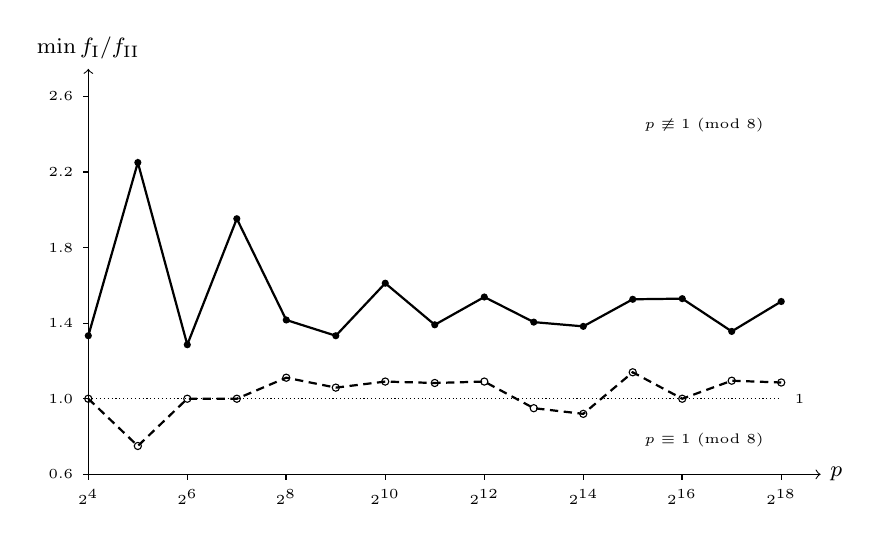
\begin{tikzpicture}[x=1cm,y=1cm]
\draw[->] (0,0) -- (9.30,0) node[right]{\footnotesize $p$};
\draw[->] (0,0) -- (0,5.15) node[above]{\footnotesize $\min \fI/\fII$};
\draw (0.00,0) -- (0.00,-0.07) node[below]{\tiny $2^{4}$};
\draw (1.26,0) -- (1.26,-0.07) node[below]{\tiny $2^{6}$};
\draw (2.51,0) -- (2.51,-0.07) node[below]{\tiny $2^{8}$};
\draw (3.77,0) -- (3.77,-0.07) node[below]{\tiny $2^{10}$};
\draw (5.03,0) -- (5.03,-0.07) node[below]{\tiny $2^{12}$};
\draw (6.29,0) -- (6.29,-0.07) node[below]{\tiny $2^{14}$};
\draw (7.54,0) -- (7.54,-0.07) node[below]{\tiny $2^{16}$};
\draw (8.80,0) -- (8.80,-0.07) node[below]{\tiny $2^{18}$};
\draw (0,0.00) -- (-0.07,0.00) node[left]{\tiny 0.6};
\draw (0,0.96) -- (-0.07,0.96) node[left]{\tiny 1.0};
\draw (0,1.92) -- (-0.07,1.92) node[left]{\tiny 1.4};
\draw (0,2.88) -- (-0.07,2.88) node[left]{\tiny 1.8};
\draw (0,3.84) -- (-0.07,3.84) node[left]{\tiny 2.2};
\draw (0,4.80) -- (-0.07,4.80) node[left]{\tiny 2.6};
\draw[densely dotted] (0,0.96) -- (8.80,0.96);
\draw[thick] (0.000,1.760) -- (0.629,3.960) -- (1.257,1.646) -- (1.886,3.246) -- (2.514,1.960) -- (3.143,1.760) -- (3.771,2.427) -- (4.400,1.899) -- (5.029,2.252) -- (5.657,1.933) -- (6.286,1.879) -- (6.914,2.223) -- (7.543,2.231) -- (8.171,1.815) -- (8.800,2.195);
\draw[thick,densely dashed] (0.000,0.960) -- (0.629,0.360) -- (1.257,0.960) -- (1.886,0.960) -- (2.514,1.227) -- (3.143,1.101) -- (3.771,1.178) -- (4.400,1.160) -- (5.029,1.178) -- (5.657,0.840) -- (6.286,0.768) -- (6.914,1.296) -- (7.543,0.960) -- (8.171,1.189) -- (8.800,1.166);
\fill (0.000,1.760) circle (1.3pt);
\draw (0.000,0.960) circle (1.3pt);
\fill (0.629,3.960) circle (1.3pt);
\draw (0.629,0.360) circle (1.3pt);
\fill (1.257,1.646) circle (1.3pt);
\draw (1.257,0.960) circle (1.3pt);
\fill (1.886,3.246) circle (1.3pt);
\draw (1.886,0.960) circle (1.3pt);
\fill (2.514,1.960) circle (1.3pt);
\draw (2.514,1.227) circle (1.3pt);
\fill (3.143,1.760) circle (1.3pt);
\draw (3.143,1.101) circle (1.3pt);
\fill (3.771,2.427) circle (1.3pt);
\draw (3.771,1.178) circle (1.3pt);
\fill (4.400,1.899) circle (1.3pt);
\draw (4.400,1.160) circle (1.3pt);
\fill (5.029,2.252) circle (1.3pt);
\draw (5.029,1.178) circle (1.3pt);
\fill (5.657,1.933) circle (1.3pt);
\draw (5.657,0.840) circle (1.3pt);
\fill (6.286,1.879) circle (1.3pt);
\draw (6.286,0.768) circle (1.3pt);
\fill (6.914,2.223) circle (1.3pt);
\draw (6.914,1.296) circle (1.3pt);
\fill (7.543,2.231) circle (1.3pt);
\draw (7.543,0.960) circle (1.3pt);
\fill (8.171,1.815) circle (1.3pt);
\draw (8.171,1.189) circle (1.3pt);
\fill (8.800,2.195) circle (1.3pt);
\draw (8.800,1.166) circle (1.3pt);
\node[font=\tiny,anchor=east] at (8.70,4.44) {$p\not\equiv1\ (\mathrm{mod}\ 8)$};
\node[font=\tiny,anchor=east] at (8.70,0.43) {$p\equiv1\ (\mathrm{mod}\ 8)$};
\node[font=\tiny,anchor=west] at (8.85,0.96) {$1$};
\end{tikzpicture}
\caption{For each dyadic range $2^{k}\le p<2^{k+1}$ with $2^{k+1}\le10^{6}$, the
minimum of $\fI(p)/\fII(p)$ over the primes of that range with $\fII(p)>0$, taken
separately over $p\not\equiv1\pmod8$ (solid, filled) and $p\equiv1\pmod8$ (dashed,
hollow). The solid minimum never falls below $1.2857$; the dashed one reaches $1$ or
less seven times and falls strictly below $1$ three times. This is Conjecture
\ref{conj:main} seen across all $78\,496$ primes at once.}
\label{fig:minratio}
\end{figure}

Table \ref{tab:exc} lists all exceptions for $p\le10^{6}$, and Figure
\ref{fig:scatter} shows the cloud for $p\le3\cdot10^{4}$. In particular Conjecture
\ref{conj:main} holds for all $p\le10^{6}$. Moreover the margin $\fI(p)-\fII(p)$ over
primes $p\not\equiv1\pmod8$ grows: its minimum is $2,18,30,62,62,68$ over the ranges
$[5,10^{3})$, $[10^{3},10^{4})$, $[10^{4},10^{5})$, $[10^{5},3\cdot10^{5})$,
$[3\cdot10^{5},6\cdot10^{5})$, $[6\cdot10^{5},10^{6})$, and over the last five of these
the minimal ratio $\fI/\fII$ stays between $1.30$ and $1.40$. Figure
\ref{fig:minratio} displays the minimal ratio over all fifteen dyadic ranges
$2^{k}\le p<2^{k+1}$ with $2^{k}\ge16$ and $2^{k+1}\le10^{6}$: for
$p\not\equiv1\pmod8$ it never falls below $1.2857$ (attained at $p=101$), whereas for
$p\equiv1\pmod 8$ it reaches $1$ or less in seven of the fifteen ranges and drops
strictly below $1$ in three of them. The two curves do not come close to meeting, and
neither shows a trend towards $1$. The prime $p=5$, the only exception with
$p\not\equiv1\pmod8$, lies below the plotted range.

\begin{table}[ht]
\caption{Sharpness of Theorem \ref{thm:e5}: proportion of the local terms with a given
$e$ for which $2B(n)<A(n)$, over all primes $p\le2\cdot10^{4}$. Each column rests on
about $1\,130$ terms. The rate is $0$ exactly for $e\le5$.}\label{tab:e5}
\centering\small
\begin{tabular}{l*{10}{r}}
\toprule
$e$ & $1$ & $3$ & $5$ & $7$ & $9$ & $11$ & $13$ & $15$ & $17$ & $19$\\
 rate & $0$ & $0$ & $0$ & $4.4\%$ & $4.0\%$ & $7.3\%$ & $4.1\%$ & $10.7\%$ & $4.4\%$ & $9.3\%$\\
\midrule
$e$ & $21$ & $23$ & $25$ & $27$ & $29$ & $31$ & $33$ & $35$ & $37$ & $39$\\
 rate & $10.5\%$ & $10.0\%$ & $6.3\%$ & $9.7\%$ & $4.8\%$ & $7.9\%$ & $6.6\%$ & $10.0\%$ & $3.7\%$ & $11.0\%$\\
\midrule
$e$ & $41$ & $43$ & $45$ & $47$ & $49$ & $51$ & $53$ & $55$ & $57$ & $59$\\
 rate & $5.6\%$ & $6.7\%$ & $9.5\%$ & $10.5\%$ & $6.5\%$ & $7.7\%$ & $5.6\%$ & $9.8\%$ & $5.6\%$ & $8.3\%$\\
\bottomrule
\end{tabular}
\end{table}

The smallest counterexamples are $(p,n)=(41,12)$ for $e=7$ with $(A,B)=(4,1)$,
$(59,17)$ for $e=9$ with $(A,B)=(2,0)$, and $(29,10)$ for $e=11$ with $(A,B)=(2,0)$;
from $e=9$ onwards the smallest counterexample always has $(A,B)=(2,0)$, which is the
shape produced by Proposition \ref{prop:sharpconstr}. For $e\in\{1,3,5\}$ no failure
occurs among the $117\,817$ local terms with $p\le10^{6}$, in agreement with Theorem
\ref{thm:e5}.

\subsection{A criterion, and exactly what remains of Conjecture \ref{conj:main}}
\label{sec:criterion}

Corollary \ref{cor:reduction} and Theorem \ref{thm:e5} combine into an unconditional
inequality which isolates the unproved part of Conjecture \ref{conj:main}. Split the
window $W$ of \eqref{eq:window} according to the value of $e_{n}=4n-p$ and put
\begin{equation}\label{eq:sigmaT}
  \sigma(p):=\sum_{n\in W,\ e_{n}\le5}\bigl(2B(n)-A(n)\bigr),\qquad
  T(p):=\sum_{n\in W,\ e_{n}\ge7}\bigl(2B(n)-A(n)\bigr).
\end{equation}

\begin{theorem}\label{thm:criterion}
For every prime $p\ge7$,
\[
  \fI(p)-\fII(p)\ \ge\ \sigma(p)+T(p),
\]
and $\sigma(p)\ge0$. Moreover $\sigma(p)\ge\tau(M^{2})\ge3$ if $p\equiv3\pmod4$, where
$M=(p+1)/4$. In particular $\fI(p)>\fII(p)$ whenever $T(p)>-\sigma(p)$.
\end{theorem}

\begin{proof}
By Corollary \ref{cor:reduction}, $\fI(p)\ge2\sum_{n\in W}B(n)$ and
$\fII(p)=\sum_{n\in W}A(n)$, so $\fI(p)-\fII(p)\ge\sum_{n\in W}(2B(n)-A(n))
=\sigma(p)+T(p)$. Every term of $\sigma(p)$ is non-negative by Theorem \ref{thm:e5}.
If $p\equiv3\pmod4$ then $e_{n}=1$ occurs, at $n=M$, and there
$A(M)=B(M)=\tau(M^{2})$, contributing $\tau(M^{2})$; the term $e_{n}=5$ contributes
$\ge0$. Finally $\tau(M^{2})\ge3$ since $M\ge2$.
\end{proof}

Two features of Theorem \ref{thm:criterion} deserve comment. First, its hypothesis
involves only the window $W$, and in particular does not require computing $\fI(p)$,
whose determination involves a parameter region of size $O(p^{2})$; the same asymmetry
appears on the algorithmic side, where Dahan \cite{Dahan} observes that a
factorization-free search over the primes of $[N,2N]$ costs $O(N\log^{3}N)$ for
Type II but $\Theta(N^{2})$ for Type I. Second, and more importantly, the split
\eqref{eq:sigmaT} is \emph{exactly} at the point where Theorem \ref{thm:e5} stops
being true: by the sharpness statement there, for every odd $e$ with
$7\le e\le2\cdot10^{4}$ some local term has
$2B(n)<A(n)$, so the cut cannot be moved by that method.

Consequently Conjecture \ref{conj:main} is reduced to a single inequality.

\begin{conjecture}[The residual statement]\label{conj:residual}
Let $p>5$ be prime with $p\not\equiv1\pmod8$. Then $T(p)>-\sigma(p)$. More precisely:
\begin{enumerate}
\item[(i)] if $p\equiv3\pmod4$ then $T(p)\ge0$;
\item[(ii)] if $p\equiv5\pmod8$ then $T(p)>-\sigma(p)$.
\end{enumerate}
\end{conjecture}

By Theorem \ref{thm:criterion}, (i) implies Conjecture \ref{conj:main} for
$p\equiv3\pmod4$ with the explicit margin $\tau(M^{2})\ge3$, and (ii) implies it for
$p\equiv5\pmod8$. We checked Conjecture \ref{conj:residual} for all primes
$p\le3\cdot10^{4}$: among the $1\,632$ primes $p\equiv3\pmod4$ the quantity $T(p)$ is
non-negative \emph{without exception}, while among the $814$ primes $p\equiv5\pmod8$ it
is negative for only three, the minimum being $T(701)=-8$. The asymmetry between the
two cases is intrinsic: for $p\equiv3\pmod4$ the layer $e_{n}=1$ exists and contributes
the whole of $\tau(M^{2})$ to $\sigma(p)$, whereas for $p\equiv1\pmod4$ the smallest
layer is $e_{n}=3$ and $\sigma(p)$ is correspondingly smaller.

Theorem \ref{thm:criterion} is effective: the hypothesis $T(p)>-\sigma(p)$ can be
verified for a given $p$ by a computation in the window $W$ alone, and this
\emph{proves} Conjecture \ref{conj:main} for that $p$. Weakening it to the sufficient
condition $\sum_{e_{n}\ge7}A(n)<\sigma(p)$, which discards the non-negative
contributions $2B(n)$ with $e_{n}\ge7$, gives the coverage in Table \ref{tab:coverage}.

\begin{table}[ht]
\caption{Proportion of primes for which the sufficient condition
$\sum_{e_{n}\ge7}A(n)<\sigma(p)$ holds, so that Conjecture \ref{conj:main} is
\emph{proved} for them by Theorem \ref{thm:criterion}.}\label{tab:coverage}
\begin{tabular}{lrrrrrr}
\toprule
range & $[10^{2},10^{2.5})$ & $[10^{2.5},10^{3})$ & $[10^{3},10^{3.5})$ &
$[10^{3.5},10^{4})$ & $[10^{4},10^{4.5})$\\
\midrule
$p\equiv3\ (4)$ & $100\%$ & $96.2\%$ & $81.9\%$ & $64.5\%$ & $52.5\%$\\
$p\equiv5\ (8)$ & $36.4\%$ & $26.9\%$ & $17.1\%$ & $13.4\%$ & $11.8\%$\\
\bottomrule
\end{tabular}
\end{table}

The proportions decrease, because $\sum_{e_{n}\ge7}A(n)$ grows with $p$ while
$\sigma(p)$ grows only like a divisor function; so Theorem \ref{thm:criterion} yields
no asymptotic case of Conjecture \ref{conj:main}. It does, however, locate the
difficulty precisely: \emph{everything reduces to showing that the layers $e_{n}\ge7$
do not, in total, undo the layers $e_{n}\le5$}. Numerically the individual layers with
$e_{n}\ge7$ fail the local inequality only $0.2\%$ to $0.4\%$ of the time
(\S\ref{sec:diagnosis}), and their aggregate effect $T(p)$ is non-negative for every
$p\equiv3\pmod4$ we tested.

\subsection{Where the surplus comes from}\label{sec:diagnosis}

The following two computations locate the excess of Type I over Type II solutions.

\emph{(a) The low layers are balanced.} For $e$ fixed let
$A_{e}(p):=A\bigl((p+e)/4\bigr)$ and $B_{e}(p):=B\bigl((p+e)/4\bigr)$. Over all
$17\,982$ primes $p\le2\cdot10^{5}$ the ratios
$\sum_{p}B_{e}(p)\big/\sum_{p}A_{e}(p)$ oscillate between $0.68$ and $1.39$, with
$\sum_{e\le41}\sum_{p}B_{e}(p)\big/\sum_{e\le41}\sum_{p}A_{e}(p)=0.988$. There is a
clear pattern modulo $4$: every layer with $e\equiv3\pmod4$ (equivalently
$p\equiv1\pmod4$) has ratio $<1$, while most layers with $e\equiv1\pmod4$ have ratio
$>1$.

\emph{(b) The surplus lives in the upper part of the window.} Splitting $W$ according
to $e_{n}/n$, over all $6\,055$ primes $p\le6\cdot10^{4}$ one finds
$\sum A=437\,618$ and $\sum B=458\,219$ for $e_{n}/n\in[0,0.05)$ (ratio $1.05$),
whereas for $e_{n}/n\in[0.4,0.5)$, $[0.6,0.7)$, $[0.7,0.8)$, $[0.8,0.9)$ the values of
$\sum A$ are $10$, $6$, $2$, $2$ against $\sum B$ equal to $12\,972$, $9\,373$,
$7\,295$, $8\,268$.

Computation (b) is precisely the content of Theorems \ref{thm:Abound} and
\ref{thm:conc}: for $e_{n}/n\ge\delta$ the quantity $A(n)$ is nonzero only when
$e_{n}/n$ is one of the finitely many rationals representable as a sum of two unit
fractions with bounded smaller denominator, and the total contribution of that region
to $\fII(p)$ is $O_{\delta}(1)$ uniformly in $p$. Computation (a) shows that in the
complementary region the two divisor counts are essentially balanced.

We draw the following conclusion. \emph{The surplus of Type I over Type II solutions
is not caused by an imbalance in the distribution of the divisors of $n^{2}$ among
residue classes modulo $4n-p$; those distributions are balanced on average. It is
caused by the geometric constraint of Theorem \ref{thm:Abound}, together with the
vanishing of $A$ for $n>(p+1)/3$ (Theorem \ref{thm:ranges}).} Consequently the natural
line of attack on Conjecture \ref{conj:main} is not an equidistribution statement for
divisors in progressions, but the following counting problem.

\begin{question}\label{q:S}
Fix $0<\delta<1$. How large is
$\#\{n\in W:\ e_{n}\ge\delta n,\ A(n)>0\}$, and how does the corresponding
contribution to $\fII(p)$ compare with that of $\fI(p)$ on the same range?
\end{question}

Theorem \ref{thm:conc} answers the first half with the bound
$D(\lfloor2/\delta\rfloor)$; by Remark \ref{rem:sharp} the truth is probably
$\asymp1/\delta$.


\subsection{Partial results, and two weakenings that are false}\label{sec:partial}

We collect what is proved towards Conjecture \ref{conj:main}, and record two natural
weakenings which numerical evidence refutes.

\smallskip
\noindent\textbf{Proved.}
\begin{enumerate}
\item $\fI(p)\ge2\tau(M^{2})$ for $p\equiv3\pmod4$, $M=(p+1)/4$
(Corollary \ref{cor:tau}); equivalently, the divisor $\delta=1$ contributes
$\tau(M^{2})$ unordered Type I solutions and no Type II solution at all
(Corollary \ref{cor:smallest}).
\item $2B(n)\ge A(n)$ for $e_{n}\in\{1,3,5\}$, and for no larger $e$
(Theorem \ref{thm:e5}); by Corollary \ref{cor:reduction} this is exactly the local
form of Conjecture \ref{conj:main}.
\item $\fI(p)-\fII(p)\ge\sigma(p)+T(p)$ with $\sigma(p)\ge0$, and
$\sigma(p)\ge\tau(M^{2})$ when $p\equiv3\pmod4$ (Theorem \ref{thm:criterion}); this
proves Conjecture \ref{conj:main} for an explicit set of primes and reduces the rest
to Conjecture \ref{conj:residual}.
\item Every Type II solution satisfies $a\le(1+\sqrt{1+4p})/4$ (Corollary
\ref{cor:sqrt}), and the number of Type II solutions with $Y\le K$ is at most $D(K)$,
uniformly in $m$ and $p$ (Theorem \ref{thm:conc}). There is no Type I analogue of
either.
\end{enumerate}

\smallskip
\noindent\textbf{False.}
Theorem \ref{thm:duality} suggests grouping the two counts by the parameter $C$, which
is $c$ for a Type I solution and $a$ for a Type II solution. Both resulting stratified
inequalities fail.
\begin{enumerate}
\item[(5)] \emph{The stratum $C=1$.} The inequality
$\#\{\text{Type I}:c=1\}\ge\#\{\text{Type II}:a=1\}$ fails; the smallest counterexample
is $p=47$, where the two counts are $6$ and $7$. Among the $301$ primes $p\le2000$ it
fails for four.
\item[(6)] \emph{Every stratum.} The inequality
$\#\{\text{Type I}:c=C\}\ge\#\{\text{Type II}:a=C\}$ for all $C$ fails for $132$ of the
$301$ primes $p\le2000$; the smallest counterexample is $p=41$, $C=3$, where the counts
are $0$ and $1$.
\end{enumerate}

\smallskip
\noindent
So Conjecture \ref{conj:main} cannot be reduced to the strata of the duality, just as
\S\ref{sec:fail}(1) shows it cannot be reduced to the terms of Theorem
\ref{thm:count}. Together with \S\ref{sec:fail}(5) --- any matching of solutions
sharing a denominator reduces to the latter --- this leaves the global estimates of
\S\ref{sec:diagnosis} and \S\ref{sec:model} as the only route we can see.

\subsection{A filtered form of Conjecture \ref{conj:main}}\label{sec:filtered}

Theorem \ref{thm:duality} attaches to every solution the invariant $\delta$. Explicitly,
if $y\le z$ are the two denominators coprime to $p$ of a Type I solution then
$\delta=4y-p$, while for a Type II solution $4/p=1/x+1/(pY)+1/(pZ)$ with $Y\le Z$ one
has $\delta=4Y-1$. For $X\ge1$ put
\begin{align*}
  N_{\mathrm{I}}(X;p)&:=\#\{\text{unordered Type I solutions with }\delta\le X\},\\
  N_{\mathrm{II}}(X;p)&:=\#\{\text{unordered Type II solutions with }\delta\le X\}.
\end{align*}
Letting $X\to\infty$ recovers the unordered forms of $\fI(p)$ and $\fII(p)$, so the
following refines Conjecture \ref{conj:main}.

\begin{conjecture}[Filtered form]\label{conj:filtered}
For every prime $p>5$ with $p\not\equiv1\pmod8$ and every $X\ge1$,
\[
  N_{\mathrm{I}}(X;p)\ \ge\ N_{\mathrm{II}}(X;p).
\]
\end{conjecture}

We verified Conjecture \ref{conj:filtered} for all primes $p\le6000$. In that range the
inequality fails for exactly ten primes, namely
\[
  41,\ 89,\ 241,\ 433,\ 881,\ 1249,\ 2161,\ 3041,\ 3169,\ 4441,
\]
\emph{all of which are $\equiv1\pmod 8$}. Only the first three are exceptions to
Conjecture \ref{conj:main} itself, so Conjecture \ref{conj:filtered} is strictly
stronger; nevertheless the dichotomy modulo $8$ survives intact. We regard this as
evidence that the class $p\equiv1\pmod8$, and not merely the coarse count, is the right
locus of the phenomenon. Figure \ref{fig:filtered} shows a typical pair of step
functions and one of the failures.

\begin{figure}[ht]
\centering
% Figure 2a : filtered counts, p=1051
\begin{tikzpicture}[x=1cm,y=1cm]
\draw[->] (0,0) -- (6.75,0) node[right]{\footnotesize $X$};
\draw[->] (0,0) -- (0,4.50);
\draw (0.00,0) -- (0.00,-0.07) node[below]{\tiny 0};
\draw (1.88,0) -- (1.88,-0.07) node[below]{\tiny 100};
\draw (3.76,0) -- (3.76,-0.07) node[below]{\tiny 200};
\draw (5.65,0) -- (5.65,-0.07) node[below]{\tiny 300};
\draw (0,0.00) -- (-0.07,0.00) node[left]{\tiny 0};
\draw (0,0.99) -- (-0.07,0.99) node[left]{\tiny 9};
\draw (0,1.99) -- (-0.07,1.99) node[left]{\tiny 18};
\draw (0,2.98) -- (-0.07,2.98) node[left]{\tiny 27};
\draw (0,3.98) -- (-0.07,3.98) node[left]{\tiny 36};
\draw[thick] (0.000,0.000) -- (0.019,0.000) -- (0.019,0.111) -- (0.019,0.111) -- (0.019,0.221) -- (0.019,0.221) -- (0.019,0.332) -- (0.094,0.332) -- (0.094,0.442) -- (0.094,0.442) -- (0.094,0.553) -- (0.094,0.553) -- (0.094,0.663) -- (0.094,0.663) -- (0.094,0.774) -- (0.094,0.774) -- (0.094,0.884) -- (0.094,0.884) -- (0.094,0.995) -- (0.094,0.995) -- (0.094,1.105) -- (0.094,1.105) -- (0.094,1.216) -- (0.094,1.216) -- (0.094,1.326) -- (0.094,1.326) -- (0.094,1.437) -- (0.094,1.437) -- (0.094,1.547) -- (0.094,1.547) -- (0.094,1.658) -- (0.094,1.658) -- (0.094,1.768) -- (0.094,1.768) -- (0.094,1.879) -- (0.094,1.879) -- (0.094,1.989) -- (0.094,1.989) -- (0.094,2.100) -- (0.094,2.100) -- (0.094,2.211) -- (0.094,2.211) -- (0.094,2.321) -- (0.169,2.321) -- (0.169,2.432) -- (0.245,2.432) -- (0.245,2.542) -- (0.245,2.542) -- (0.245,2.653) -- (0.320,2.653) -- (0.320,2.763) -- (0.546,2.763) -- (0.546,2.874) -- (0.696,2.874) -- (0.696,2.984) -- (0.998,2.984) -- (0.998,3.095) -- (1.224,3.095) -- (1.224,3.205) -- (1.299,3.205) -- (1.299,3.316) -- (1.299,3.316) -- (1.299,3.426) -- (1.901,3.426) -- (1.901,3.537) -- (2.202,3.537) -- (2.202,3.647) -- (2.353,3.647) -- (2.353,3.758) -- (3.256,3.758) -- (3.256,3.868) -- (4.461,3.868) -- (4.461,3.979) -- (5.064,3.979) -- (5.064,4.089) -- (5.967,4.089) -- (5.967,4.200) -- (6.400,4.200);
\node[font=\tiny,anchor=west] at (6.46,4.20) {$N_{\mathrm{I}}$};
\draw[thick,densely dashed] (0.000,0.000) -- (0.734,0.000) -- (0.734,0.111) -- (1.562,0.111) -- (1.562,0.221) -- (2.089,0.221) -- (2.089,0.332) -- (2.240,0.332) -- (2.240,0.442) -- (3.972,0.442) -- (3.972,0.553) -- (4.047,0.553) -- (4.047,0.663) -- (4.122,0.663) -- (4.122,0.774) -- (4.198,0.774) -- (4.198,0.884) -- (4.499,0.884) -- (4.499,0.995) -- (4.951,0.995) -- (4.951,1.105) -- (5.402,1.105) -- (5.402,1.216) -- (5.779,1.216) -- (5.779,1.326) -- (6.400,1.326);
\node[font=\tiny,anchor=west] at (6.46,1.33) {$N_{\mathrm{II}}$};
\node[font=\footnotesize] at (1.41,3.91) {$p=1051$};
\end{tikzpicture}
\\[0.5em]
% Figure 2b : filtered counts, p=433
\begin{tikzpicture}[x=1cm,y=1cm]
\draw[->] (0,0) -- (6.75,0) node[right]{\footnotesize $X$};
\draw[->] (0,0) -- (0,4.50);
\draw (0.00,0) -- (0.00,-0.07) node[below]{\tiny 0};
\draw (1.88,0) -- (1.88,-0.07) node[below]{\tiny 100};
\draw (3.76,0) -- (3.76,-0.07) node[below]{\tiny 200};
\draw (5.65,0) -- (5.65,-0.07) node[below]{\tiny 300};
\draw (0,0.00) -- (-0.07,0.00) node[left]{\tiny 0};
\draw (0,0.93) -- (-0.07,0.93) node[left]{\tiny 2};
\draw (0,1.87) -- (-0.07,1.87) node[left]{\tiny 4};
\draw (0,2.80) -- (-0.07,2.80) node[left]{\tiny 6};
\draw (0,3.73) -- (-0.07,3.73) node[left]{\tiny 8};
\draw[thick] (0.000,0.000) -- (0.132,0.000) -- (0.132,0.467) -- (0.132,0.467) -- (0.132,0.933) -- (0.132,0.933) -- (0.132,1.400) -- (0.282,1.400) -- (0.282,1.867) -- (0.282,1.867) -- (0.282,2.333) -- (0.433,2.333) -- (0.433,2.800) -- (0.584,2.800) -- (0.584,3.267) -- (1.638,3.267) -- (1.638,3.733) -- (3.144,3.733) -- (3.144,4.200) -- (6.400,4.200);
\node[font=\tiny,anchor=west] at (6.46,4.20) {$N_{\mathrm{I}}$};
\draw[thick,densely dashed] (0.000,0.000) -- (0.132,0.000) -- (0.132,0.467) -- (0.282,0.467) -- (0.282,0.933) -- (0.358,0.933) -- (0.358,1.400) -- (0.433,1.400) -- (0.433,1.867) -- (0.584,1.867) -- (0.584,2.333) -- (1.035,2.333) -- (1.035,2.800) -- (1.186,2.800) -- (1.186,3.267) -- (1.638,3.267) -- (1.638,3.733) -- (2.240,3.733) -- (2.240,4.200) -- (6.400,4.200);
\node[font=\tiny,anchor=west] at (6.46,4.20) {$N_{\mathrm{II}}$};
\node[font=\footnotesize] at (1.41,3.91) {$p=433$};
\end{tikzpicture}
\caption{The counting functions $N_{\mathrm{I}}(X;p)$ (solid) and
$N_{\mathrm{II}}(X;p)$ (dashed). Top: $p=1051\equiv3\pmod4$, where the solid curve
dominates throughout, as Conjecture \ref{conj:filtered} predicts. Bottom:
$p=433\equiv1\pmod 8$, where the dashed curve overtakes it on the range
$119\le X\le169$, although $\fI(433)>\fII(433)$ in the end.}
\label{fig:filtered}
\end{figure}

Part of Conjecture \ref{conj:filtered} can be proved.

\begin{theorem}\label{thm:filtered}
Let $p\ge7$ be prime.
\begin{enumerate}
\item[(i)] For every $X\ge1$,
$\;N_{\mathrm{II}}(X;p)\le D\bigl(\lfloor(X+1)/4\rfloor\bigr)
=\sum_{n\le(X+1)/4}\tau(n)$, a bound independent of $p$.
\item[(ii)] If $p\equiv3\pmod4$ and $M=(p+1)/4$, then $N_{\mathrm{I}}(X;p)\ge\tau(M^{2})$
for every $X\ge1$.
\item[(iii)] Consequently, if $p\equiv3\pmod 4$ then
$N_{\mathrm{I}}(X;p)>N_{\mathrm{II}}(X;p)$ for every $X$ such that
$\sum_{n\le(X+1)/4}\tau(n)<\tau(M^{2})$. In particular this holds for all
$X\le4K+3$, where $K$ is the largest integer with $\sum_{n\le K}\tau(n)<\tau(M^{2})$;
since $\tau(M^{2})\ge3$ one always has $K\ge1$, so the conclusion holds at least for
$X\le7$.
\end{enumerate}
\end{theorem}

\begin{proof}
(i) For a Type II solution $\delta=4Y-1$ with $Y=acd$, so $\delta\le X$ is equivalent to
$Y\le(X+1)/4$; now apply Theorem \ref{thm:conc}.

(ii) By Corollary \ref{cor:tau} there are $\tau(M^{2})$ unordered Type I solutions with
$\delta=1$, and $1\le X$.

(iii) Immediate from (i) and (ii). For the last sentence, $\tau(M^{2})\ge3$ because
$M\ge2$, while $\sum_{n\le1}\tau(n)=1<3$, so $K\ge1$ and $4K+3\ge7$.
\end{proof}

For the $217$ primes $p\equiv3\pmod4$ with $7\le p\le3000$ we checked that (i) holds for
every $X$ (no violations), and that the resulting proved range $X\le4K+3$ has median
$19$ and maximum $79$. Thus Theorem \ref{thm:filtered} settles an initial segment of
Conjecture \ref{conj:filtered}, of length growing with $\tau\bigl(((p+1)/4)^{2}\bigr)$;
what it does not control is the tail, where $N_{\mathrm{II}}$ eventually catches up with
$\tau(M^{2})$.

\subsection{A heuristic model, and the constant $3$}\label{sec:model}

We now describe a probabilistic model for $\fI$ and $\fII$ which predicts the value of
the ratio, and which we regard as the main evidence for Conjecture \ref{conj:main}.

Let $y\le z$ be the two denominators of an unordered Type I solution that are coprime
to $p$, and put $h:=\gcd(y,z)$, $y=ah$, $z=bh$ with $\gcd(a,b)=1$. In the notation of
Lemma \ref{lem:param} one has $h=cd$, and the defining equation $4abcd=p(a+b)+c$
becomes
\begin{equation}\label{eq:modelI}
  4abh-p(a+b)=c,\qquad c\mid h .
\end{equation}
Thus a Type I solution is the same thing as a triple $(a,h,c)$ with $c\mid h$ for which
\begin{equation}\label{eq:modelIb}
  b=\frac{c+pa}{4ah-p}
\end{equation}
is a positive integer coprime to $a$. Now $\#\{(a,h,c): ah=y,\ c\mid h\}
=\sum_{h\mid y}\tau(h)=\tau_{3}(y)$, and $y=ah$ satisfies $p/4<y\le3p/4$. Modelling
the divisibility in \eqref{eq:modelIb} as occurring with probability $1/(4ah-p)=1/(4y-p)$
leads to
\begin{equation}\label{eq:MI}
  M_{\mathrm{I}}(p):=\sum_{p/4<y\le3p/4}\frac{\tau_{3}(y)}{4y-p}.
\end{equation}

The same computation for Type II is instructive. With $Y\le Z$, $g=\gcd(Y,Z)$,
$Y=ag$, $Z=bg$, the equation $4abcd=cp+a+b$ becomes $4abg-a-b=cp$ with $c\mid g$, so
that a Type II solution is a triple $(a,g,c)$ with $c\mid g$ for which
$b=(cp+a)/(4ag-1)$ is a positive integer coprime to $a$. The same modelling gives
\begin{equation}\label{eq:MII}
  M_{\mathrm{II}}(p):=\sum_{Y}\frac{w_{p}(Y)}{4Y-1},\qquad
  w_{p}(Y)=\#\{(a,g,c): ag=Y,\ c\mid g,\ cp+a\ge4Y-1\},
\end{equation}
and $w_{p}(Y)=\tau_{3}(Y)$ for all $Y\le p/4$.

The two expressions \eqref{eq:MI} and \eqref{eq:MII} differ in exactly one respect,
and it is this difference which produces the surplus. In \eqref{eq:MI} the divisor
function $\tau_{3}$ is evaluated \emph{at the single scale $y\asymp p$}, and the weights
$1/(4y-p)$ run over $1,5,9,\dots$; in \eqref{eq:MII} it is evaluated \emph{at all
scales $Y\le p/4$}, with the weight $1/(4Y-1)$. Using
\[
  \sum_{n\le x}\tau_{3}(n)\sim\frac{x(\log x)^{2}}{2},\qquad
  \sum_{n\le x}\frac{\tau_{3}(n)}{n}\sim\frac{(\log x)^{3}}{6},
\]
we obtain
\begin{equation}\label{eq:constants}
  M_{\mathrm{I}}(p)\sim\frac{(\log p)^{2}}{2}\cdot\frac{\log(2p)}{4}\sim\frac{(\log p)^{3}}{8},
  \qquad
  M_{\mathrm{II}}(p)\sim\frac14\cdot\frac{(\log p)^{3}}{6}=\frac{(\log p)^{3}}{24},
\end{equation}
so that
\[
  \frac{M_{\mathrm{I}}(p)}{M_{\mathrm{II}}(p)}\longrightarrow\ \frac{1/2}{1/6}\ =\ 3 .
\]
\emph{The constant $3$ is precisely the ratio between the mean value of $\tau_{3}$ at a
single scale and its $1/n$-weighted average over all smaller scales.}

\begin{table}[ht]
\caption{The model \eqref{eq:MI}, \eqref{eq:MII} against the predicted constants
\eqref{eq:constants}.}\label{tab:model}
\begin{tabular}{rrrrrr}
\toprule
$p$ & $M_{\mathrm{I}}(p)$ & $(\log p)^{3}/8$ & $M_{\mathrm{II}}(p)$ &
$(\log p)^{3}/24$ & $M_{\mathrm{I}}/M_{\mathrm{II}}$\\
\midrule
$1\,009$     & $42.3$  & $41.4$  & $15.8$  & $13.8$  & $2.67$\\
$100\,003$   & $202.7$ & $190.8$ & $69.0$  & $63.6$  & $2.94$\\
$300\,007$   & $250.5$ & $250.7$ & $90.1$  & $83.6$  & $2.78$\\
$1\,000\,003$& $399.7$ & $329.6$ & $117.7$ & $109.9$ & $3.40$\\
\bottomrule
\end{tabular}
\end{table}

Table \ref{tab:model} shows that $M_{\mathrm{I}}$ and $M_{\mathrm{II}}$ do follow the
constants in \eqref{eq:constants}; the individual ratios fluctuate because
$M_{\mathrm{I}}(p)$ depends on $\tau_{3}$ near the single point $p$. The model is not
accurate in absolute terms --- averaged over the primes $p\in[10^{3},3\cdot10^{3}]$ one
finds $M_{\mathrm{I}}/(\fI/2)=1.73$ and $M_{\mathrm{II}}/(\fII/2)=1.80$, the model
overshooting both by a comparable factor (we have ignored the condition $\gcd(a,b)=1$
and the ordering $a\le b$) --- but the \emph{ratio} is reproduced well: over the same
primes $M_{\mathrm{I}}/M_{\mathrm{II}}=2.70$ against the true mean
$\fI/\fII=2.61$.

We are led to the following prediction.

\begin{conjecture}[$=$ Conjecture \ref{conj:ratio-intro}]\label{conj:ratio}
As $N\to\infty$,
\[
  \sum_{p\le N}\fI(p)\ \sim\ \frac{c}{8}\,N\log^{2}N,\qquad
  \sum_{p\le N}\fII(p)\ \sim\ \frac{c}{24}\,N\log^{2}N
\]
for some absolute constant $c>0$; in particular
\[
  R(N):=\frac{\sum_{p\le N}\fI(p)}{\sum_{p\le N}\fII(p)}\longrightarrow 3 .
\]
\end{conjecture}

Two comments. First, Conjecture \ref{conj:ratio} asserts in particular that
$\sum_{p\le N}\fI(p)\asymp N\log^{2}N$ with \emph{no} factor $\log\log N$; Elsholtz and
Tao \cite[after Theorem 1.1]{ElsholtzTao} write that the $\log\log N$ in their upper
bound ``arises from technical limitations to our method'' and conjecture that it should
be eliminated, and the model above is consistent with that.

Second, the data agree. Table \ref{tab:R} lists $R(N)$; a least-squares fit of the two
natural shapes to $41$ values of $N$ between $10^{3}$ and $10^{6}$ gives
\[
  R(N)\approx3.0159-\frac{3.0327}{\log N}\quad(\text{rms }0.0084),\qquad
  R(N)\approx1.9859+0.3128\log\log N\quad(\text{rms }0.0058).
\]
The second fits marginally better on the available range, but is unbounded; the first
has limit $3.016$, in agreement with the model. We do not think the comparison of
these two residuals is meaningful in itself --- see \S\ref{sec:loglog}, where
separating the numerator from the denominator gives a much sharper test --- but we do
regard the size of $R$ as the strongest available evidence for Conjecture
\ref{conj:main}: the expected margin between $\fI$ and $\fII$ is a factor of $3$, not
a hair, which is why exceptions are as rare as Table \ref{tab:exc} and Figure
\ref{fig:minratio} show.

\begin{figure}[ht]
\centering
\begin{tikzpicture}[x=1cm,y=1cm]
\draw[->] (0,0) -- (9.10,0) node[right]{\footnotesize $N$};
\draw[->] (0,0) -- (0,4.90) node[above]{\footnotesize $R(N)$};
\draw (0.00,0) -- (0.00,-0.07) node[below]{\tiny $10^{3}$};
\draw (2.87,0) -- (2.87,-0.07) node[below]{\tiny $10^{4}$};
\draw (5.73,0) -- (5.73,-0.07) node[below]{\tiny $10^{5}$};
\draw (8.60,0) -- (8.60,-0.07) node[below]{\tiny $10^{6}$};
\draw (0,0.00) -- (-0.07,0.00) node[left]{\tiny 2.5};
\draw (0,0.77) -- (-0.07,0.77) node[left]{\tiny 2.6};
\draw (0,1.53) -- (-0.07,1.53) node[left]{\tiny 2.7};
\draw (0,2.30) -- (-0.07,2.30) node[left]{\tiny 2.8};
\draw (0,3.07) -- (-0.07,3.07) node[left]{\tiny 2.9};
\draw (0,3.83) -- (-0.07,3.83) node[left]{\tiny 3.0};
\draw[densely dotted] (0,3.83) -- (8.60,3.83) node[right]{\tiny $3$};
\draw[thick] (0.000,0.589) -- (0.143,0.645) -- (0.287,0.698) -- (0.430,0.750) -- (0.573,0.800) -- (0.717,0.848) -- (0.860,0.895) -- (1.003,0.941) -- (1.147,0.985) -- (1.290,1.028) -- (1.433,1.070) -- (1.577,1.111) -- (1.720,1.150) -- (1.863,1.189) -- (2.007,1.226) -- (2.150,1.263) -- (2.293,1.298) -- (2.437,1.333) -- (2.580,1.366) -- (2.723,1.399) -- (2.867,1.431) -- (3.010,1.462) -- (3.153,1.492) -- (3.297,1.522) -- (3.440,1.551) -- (3.583,1.579) -- (3.727,1.607) -- (3.870,1.634) -- (4.013,1.660) -- (4.157,1.686) -- (4.300,1.711) -- (4.443,1.736) -- (4.587,1.760) -- (4.730,1.784) -- (4.873,1.807) -- (5.017,1.829) -- (5.160,1.852) -- (5.303,1.873) -- (5.447,1.895) -- (5.590,1.915) -- (5.733,1.936) -- (5.877,1.956) -- (6.020,1.975) -- (6.163,1.995) -- (6.307,2.013) -- (6.450,2.032) -- (6.593,2.050) -- (6.737,2.068) -- (6.880,2.085) -- (7.023,2.103) -- (7.167,2.119) -- (7.310,2.136) -- (7.453,2.152) -- (7.597,2.168) -- (7.740,2.184) -- (7.883,2.199) -- (8.027,2.214) -- (8.170,2.229) -- (8.313,2.244) -- (8.457,2.258) -- (8.600,2.272);
\draw[thick,densely dashed] (0.000,0.693) -- (0.143,0.733) -- (0.287,0.772) -- (0.430,0.810) -- (0.573,0.848) -- (0.717,0.885) -- (0.860,0.922) -- (1.003,0.958) -- (1.147,0.994) -- (1.290,1.029) -- (1.433,1.063) -- (1.577,1.097) -- (1.720,1.131) -- (1.863,1.164) -- (2.007,1.196) -- (2.150,1.229) -- (2.293,1.260) -- (2.437,1.292) -- (2.580,1.323) -- (2.723,1.353) -- (2.867,1.383) -- (3.010,1.413) -- (3.153,1.443) -- (3.297,1.472) -- (3.440,1.500) -- (3.583,1.529) -- (3.727,1.557) -- (3.870,1.585) -- (4.013,1.612) -- (4.157,1.639) -- (4.300,1.666) -- (4.443,1.692) -- (4.587,1.719) -- (4.730,1.744) -- (4.873,1.770) -- (5.017,1.795) -- (5.160,1.821) -- (5.303,1.845) -- (5.447,1.870) -- (5.590,1.894) -- (5.733,1.918) -- (5.877,1.942) -- (6.020,1.966) -- (6.163,1.989) -- (6.307,2.013) -- (6.450,2.035) -- (6.593,2.058) -- (6.737,2.081) -- (6.880,2.103) -- (7.023,2.125) -- (7.167,2.147) -- (7.310,2.169) -- (7.453,2.190) -- (7.597,2.212) -- (7.740,2.233) -- (7.883,2.254) -- (8.027,2.274) -- (8.170,2.295) -- (8.313,2.315) -- (8.457,2.336) -- (8.600,2.356);
\fill (0.000,0.622) circle (1.2pt);
\fill (0.216,0.761) circle (1.2pt);
\fill (0.430,0.766) circle (1.2pt);
\fill (0.645,0.967) circle (1.2pt);
\fill (0.860,0.920) circle (1.2pt);
\fill (1.075,1.143) circle (1.2pt);
\fill (1.290,1.066) circle (1.2pt);
\fill (1.505,1.117) circle (1.2pt);
\fill (1.720,1.123) circle (1.2pt);
\fill (1.935,1.055) circle (1.2pt);
\fill (2.150,1.164) circle (1.2pt);
\fill (2.365,1.231) circle (1.2pt);
\fill (2.580,1.314) circle (1.2pt);
\fill (2.795,1.296) circle (1.2pt);
\fill (3.010,1.417) circle (1.2pt);
\fill (3.225,1.421) circle (1.2pt);
\fill (3.440,1.518) circle (1.2pt);
\fill (3.655,1.535) circle (1.2pt);
\fill (3.870,1.609) circle (1.2pt);
\fill (4.085,1.633) circle (1.2pt);
\fill (4.300,1.672) circle (1.2pt);
\fill (4.515,1.720) circle (1.2pt);
\fill (4.730,1.756) circle (1.2pt);
\fill (4.945,1.813) circle (1.2pt);
\fill (5.160,1.840) circle (1.2pt);
\fill (5.375,1.886) circle (1.2pt);
\fill (5.590,1.900) circle (1.2pt);
\fill (5.805,1.942) circle (1.2pt);
\fill (6.020,1.954) circle (1.2pt);
\fill (6.235,1.992) circle (1.2pt);
\fill (6.450,2.024) circle (1.2pt);
\fill (6.665,2.067) circle (1.2pt);
\fill (6.880,2.103) circle (1.2pt);
\fill (7.095,2.134) circle (1.2pt);
\fill (7.310,2.171) circle (1.2pt);
\fill (7.525,2.198) circle (1.2pt);
\fill (7.740,2.224) circle (1.2pt);
\fill (7.955,2.261) circle (1.2pt);
\fill (8.170,2.297) circle (1.2pt);
\fill (8.385,2.329) circle (1.2pt);
\fill (8.600,2.356) circle (1.2pt);
\node[font=\tiny,anchor=west] at (6.74,1.77) {$a-b/\log N$};
\node[font=\tiny,anchor=west] at (5.30,2.09) {$a'+b'\log\log N$};
\end{tikzpicture}
\caption{The ratio $R(N)$ at $41$ values of $N$ between $10^{3}$ and $10^{6}$, with
the two least-squares fits and the predicted asymptote $R=3$. On this statistic alone
the two fits are comparable, the logarithmic one being marginally the better; see
\S\ref{sec:loglog} for the sharper test.}
\label{fig:R}
\end{figure}

\begin{table}[ht]
\caption{$R(N)=\sum_{p\le N}\fI(p)\big/\sum_{p\le N}\fII(p)$.}\label{tab:R}
\begin{tabular}{lrrrrrrr}
\toprule
$N$ & $1\,000$ & $1\,778$ & $3\,162$ & $5\,623$ & $10\,000$ & $17\,783$ & $31\,623$\\
$R(N)$ & $2.5811$ & $2.6254$ & $2.6455$ & $2.6518$ & $2.6749$ & $2.7003$ & $2.7181$\\
\midrule
$N$ & $31\,623$ & $56\,234$ & $100\,000$ & $177\,828$ & $316\,228$ & $562\,341$
& $1\,000\,000$\\
$R(N)$ & $2.7181$ & $2.7396$ & $2.7516$ & $2.7640$ & $2.7797$ & $2.7931$ & $2.8073$\\
\bottomrule
\end{tabular}
\end{table}

\subsection{Approaches that do not work}\label{sec:fail}
We record, with counterexamples, several natural strategies for Conjecture
\ref{conj:main} that fail; all were checked exhaustively in the stated ranges.

\begin{enumerate}
\item \emph{Termwise comparison in \eqref{eq:two-classes}.} The inequality
$B(n)\ge A(n)$ fails: among the primes $5\le p\le400$ only thirteen (namely
$7,11,13,19,31,37,43,67,79,103,127,163,211$) admit no local counterexample. The
smallest is $p=59$, $n=17$, where $A=2$ and $B=0$.
\item \emph{Termwise comparison after grouping by $e$.} Among the $721$ pairs $(p,e)$
with $p\le300$ and $e\le(p+4)/3$, exactly $50$ satisfy
$D(e,(pe+1)/4)<D(e,(p+e)/4)$, where $D(e,m)=\#\{t\mid m^{2}: t\equiv-m\ (e)\}$.
\item \emph{An explicit injection in the $(a,b)$ parametrisation.} By Lemma
\ref{lem:param},
\begin{align*}
  \fI(p)&=\#\{(a,b):\gcd(a,b)=1,\ ((-p^{-1})\bmod 4ab)\mid a+b\},\\
  \fII(p)&=\#\{(a,b):\gcd(a,b)=1,\ ((-p)\bmod 4ab)\mid a+b\}.
\end{align*}
The map
$(a,b)\mapsto(ca,b)$ with $c=(a+b)/e$ is a bijection for $p=17$, but among the $9\,092$
Type II data with $p\le2000$ its image fails to be a Type I datum in $7\,759$ cases.
\item \emph{Exploiting an asymptotic margin.} Although $R(N)\to3$ is expected, the
\emph{pointwise} ratio does not separate: over primes $5<p\le10^{6}$ with
$p\not\equiv1\pmod 8$ the minimum of $\fI/\fII$ is $1.2857$ (at $p=101$), and the
minimum over a dyadic range lies between $1.2857$ and $2.25$
(Figure \ref{fig:minratio}). It does not tend to $1$; but it is also not bounded away
from $1$ by a margin that grows, which is what an inductive argument would need.
\item \emph{Local pairing.} By Theorem \ref{thm:rigidity} a Type I and a Type II
solution share at most one denominator, and that denominator is the unique
$p$-free denominator of the Type II solution. Any proof by matching solutions that
share a denominator therefore reduces to (1), which fails.
\item \emph{Quadratic characters.} By Proposition \ref{prop:quad} a quadratic
obstruction kills $A(n)$ and $B(n)$ simultaneously, so it cannot separate the two
counts. Any argument must use characters of order $>2$.
\item \emph{Bounding the non-principal characters in Proposition \ref{prop:char}
absolutely.} Since $\tau(n^{2})\asymp\log^{2}n$ while the modulus $e_{n}$ can be as
large as $\asymp p$, the divisors of $n^{2}$ are far too sparse to equidistribute:
$\varphi(e)^{-1}\sum_{\chi\ne\chi_{0}}|R_{\chi}(n)|$ is of size $\asymp\sqrt{\tau(n^{2})}$,
larger than the main term $\tau(n^{2})/\varphi(e)$ by a factor $\asymp n/\log n$.
\end{enumerate}

In view of \S\ref{sec:diagnosis} and \S\ref{sec:model}, the two mechanisms that do
produce the surplus are the vanishing of $A$ for $n>(p+1)/3$ (Theorem
\ref{thm:ranges}) together with Theorems \ref{thm:Abound} and \ref{thm:conc}, and the
scale asymmetry expressed by \eqref{eq:constants}.

\subsection{Further questions}
\begin{enumerate}
\item Improve the pointwise bound $D(K)\ll K\log K$ of Theorem \ref{thm:conc}. By
Theorem \ref{thm:avg} the average over $p$ is only $O_{m}((\log K)^{3}\log\log K)$, and
Remark \ref{rem:sharp} suggests that even $O(K)$ is not optimal pointwise; the natural
guess is that $\#\{\text{Type II solutions}:Y\le K\}\ll_{\varepsilon}K^{\varepsilon}$ for
every $\varepsilon>0$, uniformly in $p$ and $m$. The obstruction to any elementary
improvement is that the pointwise bound already uses every algebraic constraint: for
each pair $(a,g)$ the parameter $c$ is forced, and what remains is the arithmetic
question of whether that $c$ divides $g$, which is an equidistribution statement.
\item Extend Theorem \ref{thm:e5} beyond $e\le5$ under additional hypotheses, or
determine exactly the pairs $(p,n)$ with $2B(n)<A(n)$ for $e=7$ and $e=9$ by the
method of \S\ref{sec:char}.
\item Prove an averaged form of Conjecture \ref{conj:main}, for instance
$\sum_{p\le N}\fI(p)>\sum_{p\le N}\fII(p)$ for large $N$. By \eqref{eq:two-classes}
the layers $e=1$ contribute equally to both sides, so this is a statement about the
layers $e\ge3$.
\item By Proposition \ref{prop:quad}, the difference $\fI-\fII$ is invisible at the
quadratic level. All twelve exceptions in Table \ref{tab:exc} other than $p=5$
satisfy $p\equiv1\pmod8$, i.e.\ $(2/p)=1$; the analogous phenomenon in
\cite[Prop.~1.6]{ElsholtzTao} is governed by quadratic reciprocity. Is there a
reciprocity-theoretic explanation of the exceptional set?
\end{enumerate}

\section{The double logarithm in the Elsholtz--Tao upper bound}\label{sec:loglog}

Elsholtz and Tao \cite{ElsholtzTao} prove
\begin{equation}\label{eq:etbounds}
  N\log^{2}N\ \ll\ \sum_{p\le N}\fI(p)\ \ll\ N\log^{2}N\log\log N,
  \qquad
  N\log^{2}N\ \ll\ \sum_{p\le N}\fII(p)\ \ll\ N\log^{2}N,
\end{equation}
and write that the factor $\log\log N$, which occurs for Type I but not for Type II,
``arises from technical limitations to our method (and specifically, in the
inefficient nature of the Brun--Titchmarsh inequality when applied to very short
progressions), and we conjecture that it should be eliminated''. The model of
\S\ref{sec:model} predicts the same (Conjecture \ref{conj:ratio-intro}). This section
does three things: it isolates the loss exactly, it reduces its removal to the gain of
a single logarithm, and it shows that the device by which \cite{ElsholtzTao} removes
the analogous loss on the Type II side is in fact partly available on the Type I side.

\subsection{Identities for a Type I quadruple}
We first record the algebra we shall need. Recall from Lemma \ref{lem:param} that a
Type I solution is a quadruple $(a,b,c,d)$ with $\gcd(a,b)=1$ and $4abcd=p(a+b)+c$,
and that $\delta=4acd-p$ is the invariant of Theorem \ref{thm:duality}(i); in this
section we follow \cite{ElsholtzTao} and write $f:=\delta$.

\begin{lemma}\label{lem:idents}
Let $(a,b,c,d)$ be a Type I quadruple for the prime $p\ge5$ and put $f:=4acd-p$. Then
$c\mid a+b$, and with $g:=(a+b)/c$,
\begin{equation}\label{eq:fg}
  fg=4a^{2}d+1,\qquad pg=4abd-1,\qquad (4ab)\,df=p\,(4a^{2}d+1)+f .
\end{equation}
Moreover $0<f<4acd$ and $\gcd(f,4acd)=1$. If in addition $a\le b$, then
\begin{equation}\label{eq:acdrange}
  \tfrac p4<acd\le\tfrac{2p}3,\qquad f\le p+c .
\end{equation}
\end{lemma}

\begin{proof}
From $4abcd=p(a+b)+c$ we get $c\mid p(a+b)$, and $p\nmid c$ because $p\nmid acd$ for a
Type I solution; hence $c\mid a+b$. Multiplying $fg=4a^{2}d+1$ by $c$ turns it into
$(4acd-p)(a+b)=4a^{2}cd+c$, and indeed
$4acd(a+b)-p(a+b)=4a^{2}cd+4abcd-(4abcd-c)=4a^{2}cd+c$. Multiplying $pg=4abd-1$ by $c$
returns the defining equation. The third identity follows from the second: $4abd=pg+1$,
so $(4ab)df=(pg+1)f=pgf+f=p(4a^{2}d+1)+f$.

Since $1/(acd)<4/p$ we have $acd>p/4$, i.e.\ $f>0$; and $f<4acd$ because $p>0$. Also
$\gcd(f,4acd)=\gcd(p,4acd)=1$. Finally suppose $a\le b$. Then
$2/(acd)\ge1/(acd)+1/(bcd)=4/p-1/(abdp)\ge3/p$, which gives $acd\le2p/3$. And $b\ge a$
gives $cg=a+b\ge2a$, i.e.\ $c(4a^{2}d+1)\ge2af$, i.e.\ $f\le2acd+c/(2a)$; since
$4acd=p+f$ this reads $f\le(p+f)/2+c/(2a)$, whence $f\le p+c/a\le p+c$.
\end{proof}

\subsection{The block decomposition, and exactly where the logarithm is lost}
For a dyadic parameter $C\ge1$ put
\[
  P(N;C):=\#\{(a,b,c,d):\ \text{a Type I quadruple for some prime }p\le N,\
  a\le b,\ C\le c<2C\}.
\]
By Theorem \ref{thm:parity}(i), $\fI(p)\le2\cdot\#\{\text{unordered Type I solutions}\}$,
so $\sum_{p\le N}\fI(p)\le2\sum_{C}P(N;C)$, the sum being over dyadic $C$.

\begin{lemma}\label{lem:block}
For every dyadic $C\ge1$,
\[
  \text{(i)}\quad P(N;C)\ \ll\ N\log^{2}N,
  \qquad\qquad
  \text{(ii)}\quad P(N;C)\ \ll\ \frac{N\log^{2}(2+N/C)}{\log(2C)} .
\]
\end{lemma}

\begin{proof}
By Lemma \ref{lem:idents} the quadruple is determined by $(a,c,d,f)$, since
$g=(4a^{2}d+1)/f$ and $b=cg-a$; and $f$ is a divisor of $4a^{2}d+1$. By
\eqref{eq:acdrange}, $acd\le2N/3$, so $ad\le 2N/(3C)$.

(i) For fixed $(a,d,f)$ there are at most $C$ admissible $c$, so by
\cite[Prop.~1.4]{ElsholtzTao} (applied in dyadic blocks in $a$ and $d$)
\[
  P(N;C)\ \le\ C\!\!\sum_{ad\le 2N/(3C)}\!\!\tau(4a^{2}d+1)\ \ll\ C\cdot\frac NC\log^{2}N
  \ =\ N\log^{2}N .
\]

(ii) Fix $(a,d,f)$. The primes counted are $p=4acd-f$ with $C\le c<2C$; they lie in the
residue class $-f$ modulo $4ad$, which is primitive because $\gcd(f,4ad)=1$, and in an
interval of length $4aCd$. For $C\ge3$ the Brun--Titchmarsh inequality
\cite{MontgomeryVaughan} bounds their number by
$\ll aCd/\bigl(\varphi(4ad)\log C\bigr)$, while for $C\le2$ the trivial bound $\le C$
serves. Summing, and treating the factor $ad/\varphi(4ad)$ exactly as in
\cite[(8.2)]{ElsholtzTao},
\[
  P(N;C)\ \ll\ \frac{C}{\log(2C)}\sum_{ad\le2N/(3C)}\frac{ad\,\tau(4a^{2}d+1)}{\varphi(4ad)}
  \ \ll\ \frac{C}{\log(2C)}\cdot\frac NC\log^{2}\Bigl(2+\frac NC\Bigr).\qedhere
\]
\end{proof}

Writing $C=2^{k}$ and $L=\log N$, Lemma \ref{lem:block}(ii) reads
$P(N;2^{k})\ll N(L-k\log2)_{+}^{2}/\max(1,k)$, and
$\sum_{k\le L/\log2}(L-k\log2)^{2}/k\asymp L^{2}\log L$: this harmonic sum, and nothing
else, is the $\log\log N$ of \eqref{eq:etbounds}. Two consequences are immediate.

\begin{theorem}[Localisation]\label{thm:loc}
For every $\varepsilon\in(0,1)$,
\[
  \sum_{C\ge N^{\varepsilon}}P(N;C)\ \ll\ \varepsilon^{-1}\,N\log^{2}N .
\]
Hence the factor $\log\log N$ in \eqref{eq:etbounds} arises entirely from the Type I
solutions with $c\le N^{o(1)}$, equivalently from the range in which the modulus $4ad$
of Lemma \ref{lem:block}(ii) exceeds $N^{1-o(1)}$.
\end{theorem}

\begin{proof}
Summing the bound $P(N;2^{k})\ll N(L-k\log2)_{+}^{2}/k$ over the range
$k\ge\varepsilon L/\log2$ gives
\[
  \ll\ \frac{N}{\varepsilon L}\sum_{0\le k\le L/\log2}(L-k\log2)^{2}
  \ \ll\ \varepsilon^{-1}NL^{2}. \qedhere
\]
\end{proof}

\begin{theorem}[One logarithm suffices]\label{thm:red}
Suppose that
\[
  P(N;C)\ \ll\ \frac{N\log^{2}(2+N/C)}{\log^{2}(2C)}
  \qquad\text{for every dyadic }C\text{ with }2\le C\le N .
\]
Then $\sum_{p\le N}\fI(p)\ll N\log^{2}N$, i.e.\ the factor $\log\log N$ in
\eqref{eq:etbounds} may be deleted.
\end{theorem}

\begin{proof}
The block $C=1$ is $\ll N\log^{2}N$ by Lemma \ref{lem:block}(i), while
\[
  \sum_{k\ge1}\frac{N(L-k\log2)_{+}^{2}}{(k\log2)^{2}}
  \ \ll\ NL^{2}\sum_{k\ge1}k^{-2}\ \ll\ NL^{2}. \qedhere
\]
\end{proof}

Thus the whole question is whether Brun--Titchmarsh can be improved by \emph{one}
factor of $\log(2C)$, uniformly over the family of progressions occurring here. For a
single progression Brun--Titchmarsh is essentially optimal, so any such gain must come
from the average over the $\tau(4a^{2}d+1)$ residue classes $-f$, or over the moduli
$4ad$.

\subsection{Four moduli for Type I}
On the Type II side, Elsholtz and Tao avoid the loss altogether
\cite[\S9]{ElsholtzTao}: their Type II parameters $(a,c,d,e)$ admit \emph{three}
moduli $ade$, $acd$, $ab$ whose product satisfies $(ade)(acd)(ab)^{1/2}\ll N^{2}$, so
that one of them is $O(N^{4/5})$ and Brun--Titchmarsh may be applied to a progression
that is not short. They add that ``it does not seem that a similar trick is available''
in the Type I case. The following shows that it is, in part.

\begin{proposition}[Four moduli]\label{prop:four}
Let $(a,b,c,d)$ be a Type I quadruple for $p$, with $f,g$ as in Lemma
\ref{lem:idents}, and put
\[
  q_{1}:=4ad,\qquad q_{2}:=4acf,\qquad q_{3}:=4cdf,\qquad q_{4}:=4ab .
\]
Then, in each of the following four ways, the quadruple is determined by the listed
data together with one further variable, and $p$ is confined to the stated residue
classes:
\begin{enumerate}
\item[(i)] data $(a,d,f)$, variable $c$: $\ p\equiv-f\pmod{q_{1}}$;
\item[(ii)] data $(a,c,f)$, variable $d$: $\ d$ is determined modulo $f$ by
$4a^{2}d\equiv-1$, and $p\equiv-f\pmod{4ac}$, so $p$ lies in one class modulo $q_{2}$;
\item[(iii)] data $(c,d,f)$, variable $a$: $\ a$ lies in at most $2^{\omega(f)}$
classes modulo $f$ (by $4da^{2}\equiv-1$), and $p\equiv-f\pmod{4cd}$, so $p$ lies in at
most $2^{\omega(f)}$ classes modulo $q_{3}$;
\item[(iv)] data $(a,b,g)$, variable $d$: $\ d$ is determined modulo $g$ by
$4abd\equiv1$, and $p=(4abd-1)/g$ runs through one class modulo $q_{4}$.
\end{enumerate}
\end{proposition}

\begin{proof}
All four moduli are coprime to the relevant data: $f\mid 4a^{2}d+1$ gives
$\gcd(f,2ad)=1$, and $\gcd(f,c)=\gcd(p,c)=1$ by Lemma \ref{lem:idents}. Case (i) is
$p=4acd-f$. In (ii) and (iii) the congruence $f\mid4a^{2}d+1$ determines $d$ modulo $f$
uniquely, respectively $a$ modulo $f$ up to the $2^{\omega(f)}$ square roots of
$-(4d)^{-1}$ modulo the odd number $f$; combining with $p\equiv-f$ modulo $4ac$
(resp.\ $4cd$) and the coprimality just noted gives the assertion. In (iv), $c=(a+b)/g$
is determined by the data, $pg=4abd-1$ by \eqref{eq:fg}, and as $d$ increases by $g$
the value of $p$ increases by $4ab$.
\end{proof}

One may therefore run the Brun--Titchmarsh step of Lemma \ref{lem:block}(ii) with the
modulus $\min(q_{1},q_{2},q_{3},q_{4})$, at the cost of the factor $2^{\omega(f)}$ in
case (iii). Numerically this is effective for the great majority of quadruples: for
$p\le2\cdot10^{4}$ there are $188\,400$ Type I quadruples with $a\le b$, and
$\min(q_{1},q_{2},q_{3},q_{4})\le p^{0.9}$ for $89.1\%$ of them, against $83.9\%$ for
$\min(q_{1},q_{2},q_{3})$ and $61.2\%$ for $q_{1}$ alone. It is not, however, enough,
and the reason is exactly the one identified in Theorem \ref{thm:loc}.

\begin{proposition}[The residual range]\label{prop:resid}
Let $0<\delta<\tfrac15$ and let $(a,b,c,d)$ be a Type I quadruple for $p$ with $a\le b$
and $\min(q_{1},q_{2},q_{3},q_{4})>p^{1-\delta}$. Then
\[
  c\ \ll\ p^{\delta},\qquad f\ \gg\ \max(a,d)\,p^{-\delta},\qquad
  f\ \gg\ p^{(1-3\delta)/2} .
\]
\end{proposition}

\begin{proof}
By \eqref{eq:acdrange}, $acd\asymp p$. Hence $q_{1}=4ad\asymp4p/c$, and
$q_{1}>p^{1-\delta}$ gives $c\ll p^{\delta}$. Similarly $cd\asymp p/a$ gives
$q_{3}\asymp4pf/a$, so $f\gg ap^{-\delta}$, and $ac\asymp p/d$ gives
$q_{2}\asymp4pf/d$, so $f\gg dp^{-\delta}$. Finally
$q_{1}q_{2}q_{3}=64(acd)^{2}f^{2}\ll p^{2}f^{2}$, and the left-hand side exceeds
$p^{3-3\delta}$.
\end{proof}

The three conditions of Proposition \ref{prop:resid} are consistent --- take
$a\asymp d\asymp p^{(1-\delta)/2}$, $c$ bounded and $f\asymp p^{(1-\delta)/2}$ --- so no
contradiction can be extracted, and the residual range is genuinely non-empty. In the
numerical range above, every quadruple with
$\min(q_{1},q_{2},q_{3},q_{4})>p^{0.9}$ has $c\le5$, and $76\%$ of them have $c=1$.
The four moduli therefore reach precisely as far as Theorem \ref{thm:loc} already does,
and no further: the obstruction is the range $c=O(1)$, where $p$ is confined to a
progression of bounded length to every modulus available, and where consequently no
sieve can help.

\subsection{Numerical evidence for the conjectured bound}
Table \ref{tab:loglog} lists $\sum_{p\le N}\fI(p)$ and $\sum_{p\le N}\fII(p)$, each
divided by $N\log^{2}N$, for $41$ values of $N$ between $10^{3}$ and $10^{6}$
(thirteen of them shown). The point of listing the second is that it is a
\emph{control}: by \eqref{eq:etbounds} its order of magnitude is known to be exactly
$N\log^{2}N$, so whatever shape it has is the shape of a quantity with no
$\log\log N$ in it.

The two columns have the same shape. Both decrease slowly; a least-squares fit of
$\alpha+\beta/\log N$ over the $41$ values gives $\alpha=0.1483$ for Type I and
$\alpha=0.0466$ for Type II, with root-mean-square residuals $0.0014$ and $0.0005$.
A fit of $\alpha+\beta\log\log N$ is slightly worse in both cases (residuals
$0.001442$ against $0.001360$, and $0.000541$ against $0.000474$), but the residuals are
not the point: the fitted slopes are \emph{negative}, $\beta=-0.045$ for Type I and
$\beta=-0.025$ for Type II. A genuine factor $\log\log N$ in $\sum_{p\le N}\fI(p)$ would
force a positive slope here; the data give the opposite sign, and give it equally for
Type II, where the absence of the factor is a theorem. We regard this as the strongest numerical
statement available at this range.

It should be said what the data do \emph{not} show. The ratio $R(N)$ of
\S\ref{sec:model} is a quotient of the two columns, and there the small residuals
compound: over the same $41$ values a fit of $a-b/\log N$ to $R(N)$ has
root-mean-square residual $0.0084$ against $0.0058$ for a fit of
$a'+b'\log\log N$, so $R(N)$ alone does not distinguish a finite limit from
logarithmic growth (Figure \ref{fig:R}). It is only after separating the numerator and
the denominator, and using Type II as a control, that the data speak.

\begin{table}[t]
\centering\small
\begin{tabular}{rrrr}
\toprule
$N$ & $\sum_{p\le N}\fI(p)$ & $\sum_{p\le N}\fI(p)\big/N\log^{2}N$
& $\sum_{p\le N}\fII(p)\big/N\log^{2}N$\\
\midrule
$1\,000$ & $10\,056$ & $0.2107$ & $0.0816$\\
$1\,778$ & $20\,691$ & $0.2078$ & $0.0792$\\
$3\,162$ & $41\,408$ & $0.2016$ & $0.0762$\\
$5\,623$ & $84\,072$ & $0.2005$ & $0.0756$\\
$10\,000$ & $165\,358$ & $0.1949$ & $0.0729$\\
$17\,783$ & $328\,311$ & $0.1928$ & $0.0714$\\
$31\,623$ & $642\,741$ & $0.1893$ & $0.0696$\\
$56\,234$ & $1\,269\,719$ & $0.1888$ & $0.0689$\\
$100\,000$ & $2\,468\,551$ & $0.1862$ & $0.0677$\\
$177\,828$ & $4\,790\,527$ & $0.1843$ & $0.0667$\\
$316\,228$ & $9\,271\,148$ & $0.1828$ & $0.0658$\\
$562\,341$ & $17\,833\,719$ & $0.1809$ & $0.0648$\\
$1\,000\,000$ & $34\,276\,271$ & $0.1796$ & $0.0640$\\
\bottomrule
\end{tabular}
\caption{The two aggregates against $N\log^{2}N$. For Type II the order
$N\log^{2}N$ is a theorem of \cite{ElsholtzTao}; the Type I column has the same
shape.}
\label{tab:loglog}
\end{table}

\begin{thebibliography}{99}

\bibitem{Aigner}
A.~Aigner,
\emph{Br\"uche als Summe von Stammbr\"uchen},
J. Reine Angew. Math. \textbf{214/215} (1964), 174--179.

\bibitem{BBF}
M.~Bello-Hern\'andez, M.~Benito and E.~Fern\'andez,
\emph{A divisor parametrization for the Erd\H{o}s--Straus conjecture},
preprint (2026), arXiv:2606.10922.

\bibitem{Bernstein}
L.~Bernstein,
\emph{Zur L\"osung der diophantischen Gleichung $m/n=1/x+1/y+1/z$, insbesondere im
Fall $m=4$},
J. Reine Angew. Math. \textbf{211} (1962), 1--10.

\bibitem{Bradford1}
K.~Bradford,
\emph{A note on the Erd\H{o}s--Straus conjecture}, Integers \textbf{21}
(2021), \#A24, 10 pp.; \texttt{doi:10.5281/\allowbreak zenodo.\allowbreak 10807535}; arXiv:1906.00561.

\bibitem{Bradford2}
K.~Bradford,
\emph{Elementary patterns from the Erd\H{o}s--Straus conjecture},
Integers \textbf{25} (2025), \#A54, 10 pp.;
preprint version: \emph{Elemental patterns from the Erd\H{o}s--Straus conjecture},
arXiv:2403.16047.

\bibitem{Chamberland}
M.~Chamberland,
\emph{The Erd\H{o}s--Straus conjecture and the structure of primes},
Integers \textbf{26} (2026), \#A42, 7 pp.
\texttt{doi:10.5281/zenodo.19403738}.

\bibitem{Dahan}
B.~Dahan,
\emph{Sieve dimension and search depth for the Erd\H{o}s--Straus conjecture,
$n\equiv1\pmod{24}$},
preprint (2026), arXiv:2608.24035.

\bibitem{ElsholtzPlanitzer}
C.~Elsholtz and S.~Planitzer,
\emph{The number of solutions of the Erd\H{o}s--Straus equation and sums of $k$ unit
fractions},
Proc. Roy. Soc. Edinburgh Sect. A \textbf{150} (2020), no.~3, 1401--1427;
arXiv:1805.02945.

\bibitem{ElsholtzTao}
C.~Elsholtz and T.~Tao,
\emph{Counting the number of solutions to the Erd\H{o}s--Straus equation on unit
fractions},
J. Aust. Math. Soc. \textbf{94} (2013), no.~1, 50--105;
arXiv:1107.1010.

\bibitem{Guy}
R.~K.~Guy,
\emph{Unsolved Problems in Number Theory}, 3rd ed.,
Problem Books in Mathematics, Springer, New York, 2004; \S D11.

\bibitem{Lopez}
M.~A.~L\'opez,
\emph{Structure and form of the solutions of the Erd\H{o}s--Straus conjecture},
preprint (2024), arXiv:2206.10319v4.

\bibitem{MihneaDumitru}
S.~Mihnea and B.~C.~Dumitru,
\emph{Further verification and empirical evidence for the Erd\H{o}s--Straus
conjecture},
preprint (2025), arXiv:2509.00128.

\bibitem{MonksVelingker}
M.~Monks and A.~Velingker,
\emph{On the Erd\H{o}s--Straus conjecture: properties of solutions to its underlying
Diophantine equation},
unpublished manuscript dated 23 September 2008, originating in a 2004--2005 Siemens
Westinghouse competition entry; available from the first author's page,
\url{http://mathematicalgemstones.com/maria/papers/ErdosStraus.pdf}.

\bibitem{MontgomeryVaughan}
H.~L.~Montgomery and R.~C.~Vaughan,
\emph{The large sieve},
Mathematika \textbf{20} (1973), 119--134.

\bibitem{Mordell}
L.~J.~Mordell,
\emph{Diophantine Equations},
Pure and Applied Mathematics, vol.~30, Academic Press, London--New York, 1969.

\bibitem{Oblath}
R.~Obl\'ath,
\emph{Sur l'\'equation diophantienne $4/n=1/x_{1}+1/x_{2}+1/x_{3}$},
Mathesis \textbf{59} (1950), 308--316.

\bibitem{Rosati}
L.~Rosati,
\emph{Sull'equazione diofantea $4/n=1/x_{1}+1/x_{2}+1/x_{3}$},
Boll. Un. Mat. Ital. (3) \textbf{9} (1954), 59--63.

\bibitem{Salez}
S.~E.~Salez,
\emph{The Erd\H{o}s--Straus conjecture: new modular equations and checking up to
$N=10^{17}$},
preprint (2014), arXiv:1406.6307.

\bibitem{Schinzel1956}
A.~Schinzel,
\emph{Sur quelques propri\'et\'es des nombres $3/n$ et $4/n$, o\`u $n$ est un nombre
impair},
Mathesis \textbf{65} (1956), 219--222.

\bibitem{Schinzel}
A.~Schinzel,
\emph{On sums of three unit fractions with polynomial denominators},
Funct. Approx. Comment. Math. \textbf{28} (2000), 187--194.

\bibitem{Sierpinski}
W.~Sierpi\'nski,
\emph{Sur les d\'ecompositions de nombres rationnels en fractions primaires},
Mathesis \textbf{65} (1956), 16--32.

\bibitem{Terzi}
D.~G.~Terzi,
\emph{On a conjecture by Erd\H{o}s--Straus},
Nordisk Tidskr. Informationsbehandling (BIT) \textbf{11} (1971), 212--216.

\bibitem{Vaughan}
R.~C.~Vaughan,
\emph{On a problem of Erd\H{o}s, Straus and Schinzel},
Mathematika \textbf{17} (1970), 193--198.

\bibitem{Webb}
W.~A.~Webb,
\emph{On $4/n=1/x_{1}+1/x_{2}+1/x_{3}$},
Proc. Amer. Math. Soc. \textbf{25} (1970), no.~3, 578--584.

\bibitem{Xu}
X.~Xu,
\emph{Congruence classes supporting the Erd\H{o}s--Straus conjecture I: tame
solutions},
preprint (2026), arXiv:2605.23601.

\bibitem{Yamamoto}
K.~Yamamoto,
\emph{On the Diophantine equation $4/n=1/x+1/y+1/z$},
Mem. Fac. Sci. Kyushu Univ. Ser. A \textbf{19} (1965), 37--47.

\end{thebibliography}

\end{document}
